\def\mytitle{College, Deliberately}
\def\myauthor{Peter Bradley}

 
\def\mysubtitle{A Guide for the Intentional Student}
 
\documentclass[nobib]{tufte-book}

\title{\mytitle}
%\subtitle{\subtitle}
\author{\myauthor}


\usepackage{booktabs}
%\usepackage{natbib}
%\usepackage[backend=biber, bibencoding=utf8]{biblatex}
\usepackage[style=chicago-authordate, backend=biber, bibencoding=utf8]{biblatex}
\usepackage[utf8]{inputenc}

\usepackage{xifthen}
\usepackage{ifpdf}
\usepackage{ifxetex}
\usepackage{hyperref}
\usepackage{geometry}
\usepackage{ragged2e}
\usepackage{paralist}
\usepackage{textcase}
\usepackage{soul}
\usepackage{letterspace}
\usepackage{setspace}
\usepackage{bibentry}
\usepackage{optparams}
\usepackage{placeins}
\usepackage{mathpazo}
\usepackage{helvet}
\usepackage{fontenc}
\usepackage{fancyhdr}
\usepackage{xcolor}

\usepackage{rotating}
\usepackage{graphicx}
\usepackage[framed, thmmarks]{ntheorem}
\usepackage{thmtools}
\usepackage{amsmath}
\usepackage{multirow}                   % use multirow tables

\usepackage{longtable}
\usepackage{threeparttable}             % allow for notes on tables
\usepackage{dcolumn}
\usepackage{float}                      % allow for precise placement of images
\usepackage{array}
\usepackage{tabulary}                   % Support longer table cells
\usepackage{epigraph}
\usepackage{fontspec}
\usepackage{makeidx}
\addbibresource{../WBE.bib}
\DeclareBibliographyAlias{webpage}{online} 

\definecolor{ferrisred}{RGB}{186,18,43}
\definecolor{ferrsgold}{RGB}{252,201,23}

% For nicely typeset tabular material
\usepackage{booktabs}

\makeindex


%%
% For graphics / images
\usepackage{graphicx}
\usepackage{environ}
\usepackage{varioref}
\usepackage{marginfix}
\usepackage{morefloats}
\extrafloats{100}



\setkeys{Gin}{width=\linewidth,totalheight=\textheight,keepaspectratio}
\graphicspath{{graphics/}}

% The fancyvrb package lets us customize the formatting of verbatim
% environments.  We use a slightly smaller font.
\usepackage{fancyvrb}
\fvset{fontsize=\normalsize}

%%
% Prints argument within hanging parentheses (i.e., parentheses that take
% up no horizontal space).  Useful in tabular environments.
\newcommand{\hangp}[1]{\makebox[0pt][r]{(}#1\makebox[0pt][l]{)}}

%%
% Prints an asterisk that takes up no horizontal space.
% Useful in tabular environments.
\newcommand{\hangstar}{\makebox[0pt][l]{*}}

%%
% Prints a trailing space in a smart way.
\usepackage{xspace}
% Prints an epigraph and speaker in sans serif, all-caps type.
\newcommand{\openepigraph}[2]{%
  %\sffamily\fontsize{14}{16}\selectfont
  \begin{fullwidth}
  \sffamily\large
  \begin{doublespace}
  \noindent\allcaps{#1}\\% epigraph
  \noindent\allcaps{#2}% author
  \end{doublespace}
  \end{fullwidth}
}

% Inserts a blank page
\newcommand{\blankpage}{\newpage\hbox{}\thispagestyle{empty}\newpage}

\usepackage{units}

% Typesets the font size, leading, and measure in the form of 10/12x26 pc.
\newcommand{\measure}[3]{#1/#2$\times$\unit[#3]{pc}}

% Macros for typesetting the documentation
\newcommand{\hlred}[1]{\textcolor{Maroon}{#1}}% prints in red
\newcommand{\hangleft}[1]{\makebox[0pt][r]{#1}}
\newcommand{\hairsp}{\hspace{1pt}}% hair space
\newcommand{\hquad}{\hskip0.5em\relax}% half quad space
\newcommand{\TODO}{\textcolor{red}{\bf TODO!}\xspace}
\newcommand{\na}{\quad--}% used in tables for N/A cells
\providecommand{\XeLaTeX}{X\lower.5ex\hbox{\kern-0.15em\reflectbox{E}}\kern-0.1em\LaTeX}
\newcommand{\tXeLaTeX}{\XeLaTeX\index{XeLaTeX@\protect\XeLaTeX}}
% \index{\texttt{\textbackslash xyz}@\hangleft{\texttt{\textbackslash}}\texttt{xyz}}
\newcommand{\tuftebs}{\symbol{'134}}% a backslash in tt type in OT1/T1
\newcommand{\doccmdnoindex}[2][]{\texttt{\tuftebs#2}}% command name -- adds backslash automatically (and doesn't add cmd to the index)
\newcommand{\doccmddef}[2][]{%
  \hlred{\texttt{\tuftebs#2}}\label{cmd:#2}%
  \ifthenelse{\isempty{#1}}%
    {% add the command to the index
      \index{#2 command@\protect\hangleft{\texttt{\tuftebs}}\texttt{#2}}% command name
    }%
    {% add the command and package to the index
      \index{#2 command@\protect\hangleft{\texttt{\tuftebs}}\texttt{#2} (\texttt{#1} package)}% command name
      \index{#1 package@\texttt{#1} package}\index{packages!#1@\texttt{#1}}% package name
    }%
}% command name -- adds backslash automatically
\newcommand{\doccmd}[2][]{%
  \texttt{\tuftebs#2}%
  \ifthenelse{\isempty{#1}}%
    {% add the command to the index
      \index{#2 command@\protect\hangleft{\texttt{\tuftebs}}\texttt{#2}}% command name
    }%
    {% add the command and package to the index
      \index{#2 command@\protect\hangleft{\texttt{\tuftebs}}\texttt{#2} (\texttt{#1} package)}% command name
      \index{#1 package@\texttt{#1} package}\index{packages!#1@\texttt{#1}}% package name
    }%
}% command name -- adds backslash automatically
\newcommand{\docopt}[1]{\ensuremath{\langle}\textrm{\textit{#1}}\ensuremath{\rangle}}% optional command argument
\newcommand{\docarg}[1]{\textrm{\textit{#1}}}% (required) command argument
\newenvironment{docspec}{\begin{quotation}\ttfamily\parskip0pt\parindent0pt\ignorespaces}{\end{quotation}}% command specification environment
\newcommand{\docenv}[1]{\texttt{#1}\index{#1 environment@\texttt{#1} environment}\index{environments!#1@\texttt{#1}}}% environment name
\newcommand{\docenvdef}[1]{\hlred{\texttt{#1}}\label{env:#1}\index{#1 environment@\texttt{#1} environment}\index{environments!#1@\texttt{#1}}}% environment name
\newcommand{\docpkg}[1]{\texttt{#1}\index{#1 package@\texttt{#1} package}\index{packages!#1@\texttt{#1}}}% package name
\newcommand{\doccls}[1]{\texttt{#1}}% document class name
\newcommand{\docclsopt}[1]{\texttt{#1}\index{#1 class option@\texttt{#1} class option}\index{class options!#1@\texttt{#1}}}% document class option name
\newcommand{\docclsoptdef}[1]{\hlred{\texttt{#1}}\label{clsopt:#1}\index{#1 class option@\texttt{#1} class option}\index{class options!#1@\texttt{#1}}}% document class option name defined
\newcommand{\docmsg}[2]{\bigskip\begin{fullwidth}\noindent\ttfamily#1\end{fullwidth}\medskip\par\noindent#2}
\newcommand{\docfilehook}[2]{\texttt{#1}\index{file hooks!#2}\index{#1@\texttt{#1}}}
\newcommand{\doccounter}[1]{\texttt{#1}\index{#1 counter@\texttt{#1} counter}}

\renewcommand{\maketitlepage}[0]{%
  \cleardoublepage%
  {%
  \sffamily%
  \begin{fullwidth}%
  \fontsize{18}{20}\selectfont\par\noindent\textcolor{darkgray}{\allcaps{\myauthor}}%
  \vspace{11.5pc}%
  \fontsize{36}{40}\selectfont\par\noindent\textcolor{darkgray}{\allcaps{\mytitle}}%
  \fontsize{18}{20}\selectfont\par\noindent\textcolor{ferrisred}{\mysubtitle}%
  \vfill%
  \fontsize{14}{16}\selectfont\par\noindent\allcaps{\thanklesspublisher}%
  \end{fullwidth}%
  }
  \thispagestyle{empty}%
  \clearpage%
}

% part format

\titleformat{\part}%
  {\Huge\rmfamily\bfseries\color{ferrisred}}% format applied to label+text
  {\Huge\rmfamily\bfseries\color{ferrisred}\thepart}% label
  {10pt}% horizontal separation between label and title body
  {}% before the title body
  []% after the title body


  \titlecontents{part}% FIXME
    [0em] % distance from left margin
    {\vspace{1.5\baselineskip}\begin{fullwidth}\LARGE\rmfamily\itshape\color{ferrisred}} % above (global formatting of entry)
    {\contentslabel{2em}} % before w/label (label = ``II'')
    {} % before w/o label
    {\rmfamily\upshape\qquad\thecontentspage} % filler + page (leaders and page num)
    [\end{fullwidth}] % after


% Chapter format
\titleformat{\chapter}%
  {\huge\rmfamily\itshape\color{ferrisred}}% format applied to label+text
  {\llap{\colorbox{ferrisred}{\parbox{1.5cm}{\hfill\itshape\huge\color{white}\thechapter}}}}% label
  {5pt}% horizontal separation between label and title body
  {}% before the title body
  []% after the title body



% section format
\titleformat{\section}%
  {\normalfont\Large\itshape\color{ferrisred}}% format applied to label+text
  {\llap{\colorbox{ferrisred}{\parbox{1.5cm}{\hfill\color{white}\thesection}}}}% label
  {1em}% horizontal separation between label and title body
  {}% before the title body
  [\color{black}]% after the title body

% subsection format
\titleformat{\subsection}%
  {\normalfont\large\itshape\color{ferrisred}}% format applied to label+text
  {\llap{\colorbox{white}{\parbox{1.5cm}{\hfill\color{ferrisred}\thesubsection}}}}% label
  {1em}% horizontal separation between label and title body
  {}% before the title body
  [\color{black}]% after the title body

% Add subsubsection
% Add subsubsection
\makeatletter
\renewcommand{\subsubsection}{\ttl@straightclass{subsubsection}}
\makeatother
\titleformat{\subsubsection}
  {\bfseries\normalsize}
  {\thesubsubsection}
  {1em}
  {}
  []


\newcounter{purpose}
\newcounter{thesis}


\declaretheoremstyle[
  headfont=\color{ferrisred}\normalfont\bfseries,
  bodyfont=\color{black}\normalfont\itshape,
]{colored}

\declaretheorem[
  style=colored,
  name=Purpose,
shaded={rulecolor=ferrisred, rulewidth=0.5pt, bgcolor={rgb}{1,1,1}},
numberwithin=chapter
]{mypurpose}

\declaretheorem[
  style=colored,
  name=Thesis,
numberwithin=chapter
]{mythesis}

\declaretheorem[
  style=colored,
  name=Subjects,
  parent=mypurpose
]{myentities}

\declaretheorem[
  style=colored,
  name=Object,
  parent=mypurpose
]{myobjects}

\declaretheorem[
  style=colored,
  name=Discussion Question,
shaded={rulecolor=black, rulewidth=0.5pt, bgcolor={rgb}{1,1,1}} 
]{myquestion}

% \newtheorem{theorem}{Definition}[chapter]

\makeatletter
\NewEnviron{purpose}[1][]{
\refstepcounter{purpose} 
\protected@edef\@currentlabelname{#1}% addition here
\noindent \marginnote{
 \begin{mypurpose}[#1]\BODY\end{mypurpose}
 }
}
\numberwithin{mypurpose}{chapter}

\NewEnviron{question}[1][]{
\protected@edef\@currentlabelname{#1}% addition here
\noindent \marginnote{
 \begin{myquestion}\BODY\end{myquestion} 
}}

\NewEnviron{thesis}[1][]{
\refstepcounter{thesis}
\protected@edef\@currentlabelname{#1}% addition here
 \noindent \marginnote{
 \begin{mythesis}[#1]\BODY\end{mythesis}
}
}
\numberwithin{thesis}{chapter}

\NewEnviron{entities}[1][]{\protected@edef\@currentlabelname{#1}% addition here
\noindent \marginnote{
 \begin{myentities}[#1]\BODY\end{myentities}
}}

\NewEnviron{objects}[1][]{\protected@edef\@currentlabelname{#1}% addition here
\noindent \marginnote{
 \begin{myobjects}[#1]\BODY\end{myobjects}
}}

\makeatother

% Bug fix - https://groups.google.com/forum/#!msg/tufte-latex-commits/JcgGP-1R138/-Srf_tzAKHkJ
% Set up the spacing using fontspec features
\renewcommand\allcapsspacing[1]{{\addfontfeature{LetterSpace=15}#1}}
\renewcommand\smallcapsspacing[1]{{\addfontfeature{LetterSpace=10}#1}}
% https://abnormaldata.wordpress.com/2015/01/14/configuring-scrivener-latex/
\ifx\citep\undefined
   \let\citep\cite
   \let\citet\cite
\else
   \renewcommand\citep{\cite}
   \renewcommand\citet{\cite}
\fi




%\newcommand{\fullref}[1]{\hyperref[{#1}]{\autoref*{#1} \nameref*{#1}}}
\newcommand*{\tahead}[1]{{\bfseries #1}} % Table header
\newcommand*{\thead}[1]{{\bfseries #1}} % Table header
\newcolumntype{P}[1]{>{\raggedright\arraybackslash}p{#1}}
\newcolumntype{R}[1]{>{\raggedleft\arraybackslash}p{#1}}



%\ldots
\newcolumntype{d}[1]{D{.}{\cdot}{#1} } % Define table column

\pagestyle{plain}


\setcounter{tocdepth}{1}

% Set numbering system to sub subsection

% Generates the index
\usepackage{makeidx}
\makeindex

\begin{document}
\maketitle

% Front matter
\frontmatter\pagenumbering{roman}\pagestyle{empty}



 \chapter{To the student:}

\marginnote{\emph{In college, you have to do it on purpose.} \newline -Ferris State Honors Alumna Rachel LaBrecque}

Let us begin with a deceitfully simple question: Why are you in college?

If you are like most American students today, your answer will be something like ``to get a job,'' or ``to have a good career.'' But think about that answer for a moment. It's a pretty superficial answer. Why this particular career? Who made college a prerequisite for this career? Why this particular college? 

Answering the question ``Why are you in college?'' with ``to get a job'' is like asking ``Why are you eating pizza for dinner?'' with ``because I need to take in calories to survive.'' It answers part of the question, certainly, but ignores the layers of social, cultural and economic forces at play in your choice of this pizza at this moment.

Was pizza the only choice available? What is the cost of pizza relative to other options? Does pizza have a special role in your culture--as it is usually shared between many people, perhaps having pizza serves to reinforce social bonds? Were you raised in a society that has regular access to pizza, or is pizza something that only the very few have on special occasions? Did you grow up in St. Louis, where pizza is nasty?\footnote{Sorry, St. Louis. I spent my post-doc years in University City, and while I love your city very much and appreciate your many cultural offerings such as your world-class zoo, fabulous Universities, wonder-of-the-world City Museum (where I was married), and forest park, your pizza is just intolerable.}

The response ``to get a job'' contains social, cultural and economic background conditions which demand our attention. Is college expected of you? Are you going to a public, secular college or a private, religious one? A traditional liberal arts college, or a technical or vocational college? Are you going to college to be better off financially? Did you pick a college that was close to home, or did you explore colleges nation-wide? Are you going to the same college your parents---or your grandparents---attended? What about colleges in other countries?

In recent years, the ways Americans have answered these questions have changed. When college was once seen as a place where young people were able to explore ideas with a luxurious freedom from economic pressure, it is now seen almost exclusively as an investment in a students' future career.

For example, in 1973, only 37.1\% of incoming first-year students at UCLA claimed that they were attending college ``to be better off financially.'' 72.7\% responded that they were interested in ``developing a meaningful philosophy of life.''\footnote{The UCLA survey allowed student to check more than one reason for attending college, so the percentages herein will not add up to 100.} By 2013, these rates had flipped: 82\% want to be better off financially, while 44.8\% want to develop a philosophy of life.\footnote{Cited in~\citep{Berrett:2015ui}, the original study is available for download. See ~\citep{Eagen:2016vk}}

In 2011, the Pew Research organization surveyed the American public regarding the purpose of college. 47\% of respondents said ``teach knowledge or skills that would be useful in the workplace'' and 39\% said ``help individuals grow personally.'' An addition 12\% said ``both purposes equally.''\footnote{~\citep{PewResearchCenter:2011vl}} 

The word `career'---or one of its commonly used variants---is the 10th most frequently used word in a corpus of the 4,264 websites of English-speaking Colleges and Universities in the US.\footnote{The corpus in question was built during Fall 2016 by the author using the statistical software R and the package `Quanteda'. See ~\citep{Packagequanteda:wb} for more. Technical details of the study can be found in the Appendix.} It is slightly more frequent in two year colleges (7th place) than in four year colleges (11th place).\footnote{The frequency of `career' does vary a little on based on the College's selectivity (Carnegie variable ACTCAT: highly selective: 19th, selective: 13th, and nonselective 9th), and the funding model (private for profit: 7th, private not for profit: 13th, public 14th). It is notable that traditional Liberal arts institutions---Carneige classification CC2000---and faith-based institutions do not mention `career' in their top 20. I will return to this dataset in later chapters.}

As a culture, the American College system has spawned entire industries worth millions of dollars. College entrance testing, prep guides, college guides and rankings generate millions. College sports generate billions of dollars annually\footnote{See, for example ~\citep{Humphreys:2008wr}}, little to none of which actually supports learning inside or outside the classroom\footnote{See, e.g. ~\citep{DavidWelchSuggs:2012wf} and ~\citep{Wolverton:2015uy}}. 

Back in about 400 BCE, Socrates proclaimed that the ``unexamined life is not worth living.'' Philosophers have always regarded Socrates' dictum as a duty of our profession. We cajole society---sometimes to our own fault---into examining their lives, making decisions and taking actions deliberately, based on reason. We are supposed to be the ones shouting ``The emperor has no clothes!'' from the throngs of the compliant. 

This book is in that tradition. 

Somewhere between 1973 and 2013, the understanding of why we go to college shifted. Dramatically. It is my job, as a Philosopher, to poke at this shift in order to expose it for all to see.

I am not the only one asking questions about the purpose of college in our society. As we'll see, there have been billionaires like Peter Thiel, and brilliant philosophers like Martha Nussbaum engaged in a spirited public debate on the role and meaning of college. But their arguments appear to have little impact on the industry of college guides and college preparation.

College guides typically speak in undocumented and unsupported platitudes. College rankings generally measure features of a college or university that are self-fulfilling (such as admissions standards) or irrelevant to the students' experience in the classroom. There is little data---and far less critical thinking---in this industry.

Don't worry. A philosopher is here to help.

\section*{The purposes of this book} 

In this book, we will look at various different approaches to the question of why a person---or a society---might benefit from a college education. We reach back to the very foundation of Western Civilization in ancient Athens, and trace concepts from their origination to their expression in modern day collegiate mission statements, vision and value statements, strategic plans and marketing materials.

Different colleges have different purposes---why they exist, and what they intend to `produce' in a successful student. But this is rarely, if ever, discussed in the process of choosing a College. This strikes me as odd. If a student truly believes that self-understanding is the ultimate purpose of college, would he or she not be advantaged to know which colleges take that as their primary mission? 

This book is help students understand the institutions they inhabit---or will inhabit. It is written to facilitate discussion about the purpose or end of College between students, guidance counselors, professors and in the culture generally. It does not advance a particular thesis on the purpose of college other than ``There are multiple overlapping purposes to college in American culture.''\footnote{One might argue that there is an overarching thesis to the book that is something like: ``if students and parents better understand the multiple overlapping purposes of college in American culture, and understand where different colleges lie in that spectrum of overlapping purposes; then they might make better, more informed and more deliberate decision about College. And that's a good thing.'' Fair enough. But I don't pretend to present any evidence beyond the anecdotal that these discussions will, \emph{in fact}, cause better decisions.}

I've been talking about the purpose of college for about a decade, and during that time, have had multiple chances to present my ideas before an assembly of high school and junior high school students. In every case, students stayed after to thank me for the insights they gained during the presentation. I sincerely hope that you will feel the same after completing this book.

The first part of the book addresses what it means to advance a theory of higher education, and why this question is so important today.

The second part presents eight purposes of education, each expressed in a major work of western civilization---a `core text'\footnote{I make no claims that the set of `great texts' the book assumes is ``the'' canon or any such nonsense. My claim is merely that actual existing institutions of higher learning in the US by and large trace their intellectual genealogy to this collection of works. And to better understand our own cultural institutions and assumptions, we must return to these works, and attempt to understand them as their advocates once did. We may agree with these texts. We may disagree with them. We may be frustrated that the founders of our institutions praised these texts while ignoring others. But none of that is relevant to my project in this book. The fact is that our institutions inhabit a conceptual tradition that I wish to trace. And so, I trace it through the canon.} if you will---and found in today's vision, mission and strategic plans of US colleges and universities.

Used as a supplement to the major works in a ``Great Books'' or ``Core Texts'' course, the book will enhance the students' understanding of the institutions and contexts of higher learning in the US: what college education is for, and how contemporary discourse links to antecedents in the Western canon. Table \ref{table: readings} contains the readings I have used teaching this theme. Each of the corresponding chapters begins with a problem posed by these texts.

 \begin{longtable}[!t]{ | p{4cm} | P{6.5cm} |   }
\hline 

\thead{Chapter} & \thead{Reading}\\ \hline
Chapter \ref{introduction}: \nameref{introduction}&DuBois, \emph{The Souls of Black Folk}, especially "On the Coming of John"\\ \hline
Chapter \ref{forvocation}: \nameref{forvocation}&
Pestalozzi, \emph{How Gertrude Teaches her Children}, excerpts\newline
Comte, \emph{Introduction to Positive Philosophy}\newline
Spencer, \emph{Education}, Chapter 1, selections from Ch. 4 (235-306)\newline
Crawford, \emph{Shopclass as Soulcraft}, \newline 
selections from Booker T. Washington  \emph{Up From Slavery}, \newline 
DuBois, "Of Booker T. Washington and Others" (in \emph{Souls})\\ \hline
 Chapter \ref{forstatecraft}: \nameref{forstatecraft}&
Plato,  \emph{Republic}; 
\newline selections from Locke \emph{Some thoughts concerning education} and Dewey \emph{Democracy and Education},  http://historymatters.gmu.edu/d/4929/ \newline 
DuBois "Of our Spiritual Strivings" (in \emph{Souls})\\ \hline
 Chapter \ref{forcharacter}: \nameref{forcharacter}&Aristotle,  \emph{Nicomachean Ethics} \newline selections from Rousseau \emph{\'Emile} \newline DuBois TBA \\ \hline
Chapter \ref{forgod}: \nameref{forgod}&Augustine "The Teacher", \newline Hugh of Saint Victor,  \emph{Didascalicon}, \newline DuBois "Of the Faith of the Fathers"\\ \hline
Chapter \ref{forculture}: \nameref{forculture}&Strauss, L. "What is Liberal Education?", \newline MacCauley, "Minute on Education", \newline Tagore, "The Parrot", \newline Gandhi \emph{Hind Swaraj}, \newline selection from Alexie, \emph{The Absolutely True Diary of a Part-Time Indian}, \newline DuBois "Of the Wings of Atalanta"\\ \hline
Chapter \ref{forhumanadvancement}: \nameref{forhumanadvancement}&Gandhi \emph{Hind Swaraj}, \newline DuBois "Of the Meaning of Progress"\\ \hline
Chapter \ref{forfreedom}: \nameref{forfreedom}&Dewey \emph{How we think}, \newline Mill \emph{On Liberty} \newline selections from Wollstonecraft \emph{Vindication of the Rights of Women} \newline DuBois "Of the Dawn of Freedom" \\ \hline
Chapter \ref{foraspiration}: \nameref{foraspiration}&DuBois, "Of the Training of Black Men"\\ \hline
            \caption{Suggested Supporting Readings}
\label{table: readings}
\end{longtable}

The entry in the Stanford encyclopedia of philosophy of Herbert Spencer does not mention---not once---his work on education! While DuBois is mentioned in entries on `Double Consciousness' and `Philosophy of Race', he does not have his own entry in the Stanford Encyclopedia -- and the `Talented Tenth' appears only in the `Double Consciousness' entry. 

For Locke, the SEP has entries on Locke himself, his political theory, his view on Freedom, his moral philosophy, his view on `real essence' and his view on Philosophy of science. We even have a entry on the Molyneaux problem, which appears in Locke's writing. Yet no entry on Locke's view on education. It is true that ``On education'' is one of the headings on the general `Locke' page, but it is clear that education is not a point of emphasis for the editors of the SEP.

 \newpage
\tableofcontents
\listoftables
\listoffigures
\listoftheorems[ignoreall,show={mypurpose,mythesis,myentities,myobjects}]

\setcounter{secnumdepth}{3}

\mainmatter\setcounter{page}{1}\pagenumbering{arabic}
    \fancyfoot[CE,CO]{\today} 


\part{The Problem}
\label{theproblem}

\chapter{Introduction}
\label{introduction}

In ``Of the Coming of John'' within \emph{The Souls of Black Folk}, W.E.B DuBois tells us the story of his fictional John, a bright young student from Altamaha, GA. After an initially rough start, John falls in love with education and grows ``in body and soul'' before the author's eyes. After graduation, John avoids returning to the South by travelling in the North and enjoying his freedom and youth. Ultimately, John returns to Altamaha out of his own sense of duty to his family and his people. Almost immediately, however, things go horribly wrong when John thoughtlessly belittles the distinction between Methodists and Baptists. John then finds himself on the outside of the very society that raised him and joyously anticipated his homecoming.\begin{marginfigure}\includegraphics{DuBois.jpg}\caption{W.E.B. Du Bois, Addison N. Scurlock, Gelatin Silver Print, 1911. From the National Portrait Gallery, Washington D.C. Public Domain, via Wikimedia Commons.}\label{fig:dubois}\end{marginfigure}

As he ponders his problems on the bluff overlooking the sea, his beloved younger sister asks:

\begin{quote}

``John, does it make every one -- unhappy when they study and learn lots of things?''

He paused an smiled. ``I am afraid it does,'' he said.

``And, John, are you glad you studied?''

``Yes,'' came the answer, slowly but positively.

She watched the flickering lights upon the sea, and said thoughtfully, ``I wish I was unhappy, -- and -- and,'' putting both arms about his neck, ``I think I am, a little, John.'' ~\citep[p. 149]{DuBois:1994ui}
\end{quote}

DuBois' \emph{Souls of Black Folk} is an amazing work. Its essays are wide-ranging and timeless. It is usually read with careful attention to the concepts of `double consciousness' inherent in the African-American experience and `the veil' of race that first appear in ``Of our Spiritual Strivings.'' On education, the essays ``Of Mr. Booker T. Washington and Others,'' and ``On the Training of Black Men,'' are the subject of great debate. In the second of these, DuBois speaks of education as ``education that encourages aspiration'', which ``seeks as an end culture and character rather than bread winning.'' (p. 59) 

So it is against this backdrop of literary commentary that we notice this little passage from the final chapter in \emph{Souls}---which is the only piece of fiction in the book. Yet it contains this truth, this profound illustration of the problem of education.

DuBois introduced his concept of `double consciousness' when exploring the complexity of answering the question he frequently faced: `how does it feel to be a problem?' As an African-American, he argues, one is constantly aware not only of oneself, but also of how one's self is impacting and is perceived by others.

Here, John faces a similar double consciousness, aware of the power of his own education, yet simultaneously aware of the impact his education has had on his own family.

\newthought{Ever since Socrates' dictum}, `The unexamined life is not worth living,' we educators have assumed that education is an intrinsic good. Aristotle, the greatest of the Ancient Greek Philosophers, asserted that the uneducated differ from the educated as much as the dead from the living.\footnote{As quoted Diogenes Laertius. ~\citep[p. 463]{Laertius:eqeg5o3J}} A Medieval monastic head named Hugh of Saint Victor opened his masterwork, the \emph{Didascalicon,} with the following:

\begin{quote}

Not knowing and not wishing to know are far different things. Not knowing, to be sure, springs from weakness; but contempt for knowledges springs from a wicked will.
\end{quote}

Being educated is frequently held to be, if not an imperative, preferable to being uneducated. But why? Is education an intrinsic good, or is it to be valued only in the context of some other good, such as the need for an informed electorate? Is an educated person a more moral or virtuous person than an uneducated person? Are the liberally educated somehow better people than the technically educated? Are those who grapple with the 'core texts, `great ideas,' `great books,' `great works,'\footnote{My previous institution,, McDaniel College's core sequence for its honors program} or `great conversation\footnote{Saint Olaf in Minnesota's program.}' better somehow than those with a technical or vocational education?

On some level, you have probably asked yourself these questions. Choosing a college or a degree program requires you to put a value on different opportunities. Want to study engineering? Excellent---but what if you are also interested in continuing athletics? Most tech schools don't have strong athletic offerings. Which aspect of your life do you value more? 

Want to become a lawyer? Great: do you major in pre-law, political science, criminal justice or philosophy?\footnote{See ~\citep{LSAC:2015wz}. For an example of how this data is used by Philosophy departments, see http:\slash \slash www.phil.ufl.edu\slash ugrad\slash whatis\slash LSATtable.html.} Philosophy students have the highest LSAT scores and the best placement record. But that's probably because only a small sample of all philosophy majors apply to law school---and there are probably equal numbers without clear career tracks after undergraduate out there. Philosophy is a risky bet: it could pay off really well, and it could leave you without a fall back position. How much value do you place on this decision?

Or should you just study things that are interesting to you now, the future be damned? What really matters is contentment, after all, and you know, deep down, that you won't be content unless you are able to dedicate your life to the pursuit of truth and beauty. 

When those of us who have dedicated our lives to the academy are asked to reflect on their notion of the `good life,' I suspect many would describe a life of engagement with ideas. Many of us speak fondly of the kind of intense focus that comes with sustained study on a specific topic---the kind that is usually only achieved during dissertations or sabbatical. But we cannot assume that this ideal of the good is universally shared.

Some find engaging in deep reflection taxing; and some find that entertaining ideas different from their own to be unpleasant and disorienting. Such reactions should not be dismissed as simple anti-intellectualism. As DuBois---an intellectual of the highest order---recognizes, education can be unpleasant and disorienting. But, as with John, we are happy for having been educated.

Aristotle finds the highest excellence in a life of contemplation. John Stuart Mill, the great 19th century Philosopher of Liberalism, asserts the ``unquestionable fact\footnote{The phrase ``unquestionable fact,'' when used by a philosopher, frequently means ``empirical fact I have not bothered to confirm.'' I will attempt to avoid this trap in this book by relying on my analysis of the mission, vision and value statements of American colleges and Universities, as described in the Appendix.}'' that those acquainted with both the pleasures of the mind and the pleasures of the `animal appetites' prefer the former to the latter ~\citep[p. 9]{Mill:1871vt}. So highly educated intellectuals tell us that being a highly educated intellectual is a pretty good life. Awesome. I bet if you asked Tom Brady, he would say his life is pretty damn good too.

There is at least one study that attempted to find a connection between educational level and one's conception of ``the good life.'' The study followed Mill by arranging a hierarchy of `stages' of ideas of good life, and assumed that the `higher' stages are reversible to the `lower.' ~\citep{Armon:2007vu} The author assumes, as does Mill and Aristotle, that those capable of appreciating a life of quiet reflection on ideas can of course appreciate a life of craftsmanship or husbandry. But that's not all---a hierarchy such as this assumes that the inverse is not true: one who appreciates husbandry might not be able to appreciate quiet reflection. It is then claimed that those with more education have a broader view of the `good life' than those with less.

As a result, the study fails to do anything other than establish a correlation. It cannot show if having more education makes one's view of the good life broader, or if having a broad view of the good life drives one to become educated. On the assumption that conceptions of the good life are orderly and hierarchically arranged, it seems that either hypothesis is equally plausible. 

To illustrate this, imagine a group of 100 individuals, each of whom has an innate conception of the good life. These conceptions fall into one of three types: quiet reflection, craftsmanship and animal husbandry. The 100 are placed in an American school system and exposed to a number of extra-curricular activities like Boy Scouts, Girl Scouts, 4H, etc. Now assume that each student is exposed to activities in a hierarchical order starting with craftsmanship and ending with quiet reflection. Each student who finds a match for their innate preference will stop seeking new experiences. Those who do not find such a match will continue to search. At the end of the process, only those who prefer quiet reflection remain. And what is more, they would be under the impression that they experienced the pleasures of craftsmanship and husbandry, but preferred quiet reflection; while those who preferred the others never experienced quiet reflection. And that is exactly the kind of argument we get from intellectuals like J.S. Mill.

But nowhere in the hypothetical situation is a value judgment made on whether or not any of these systems is `better' than any of the others. The educational system I have described is nothing more than a process of selection, akin to the mechanisms of natural selection that rule biological viability. The system `selects' for those with a certain innate or genetic difference, and in no way values one difference over another. The natural world does not make judgments of `good' and `right.' And so, too, with my hypothetical educational system: if the hierarchy were inverted, the craftsmen would be able to claim the broadest experience with different views of the good life.

\section{Are you glad that you study?}
\label{areyougladthatyoustudy}

Let us turn back for a moment to \emph{On the coming of John}. John's answer to his sister's question ``are you glad you studied?'' is described by DuBois using the passive voice. John does not assert, or claim, or profess or affirm. On the contrary, the answer ``came'' through no action of John's. And it came ``slowly but positively.''

A few years back, I had the opportunity to conduct a survey of my incoming first year Honors students at a small, private liberal arts college on the East Coast. I asked them to rate, using a Likert Scale, the extent they agree with the statement: ``The reason I am going to college is to get training for a job.'' That summer, I had the opportunity to teach rising seniors from the east of Anacostia high schools in Washington DC as a part of a summer `bridge' program to college. 

These two groups of students should be opposites in American higher education: one predominately wealthy, white with access to the best college preparation. The other, predominately poor and African-American with no college prep--which is precisely why they were in our `bridge' program. Their answers to my question, however, were identical: mean of 3.94 out of 5. 

The full responses\footnote{I grant that these numbers were not collected to the standard of a truly scientific study. I collected them to make a point to my students of privilege, and did not intend to ever include them in a published work. The raw data is available to review upon request.} are presented in table \ref{table: responses}.

 \begin{longtable}[!t]{ | p{6cm} | R{2.5cm} | R{2.5cm} |  }
\hline 

\thead{The reason I am going to college is:}&\thead{Private Liberal Arts (n=16)}&\thead{East of Anacostia (n=38)} \\ \hline
To learn& 4.68& 4.65\\
To be a leader in my community&3.25&4.22\\
 Because I'm expected to& 3.31 & 3.45\\
 Athletics&1.68&2.19\\
Parties&2.68&2.58 \\ \hline
\caption{Responses from students, 2010}
\label{table: responses}
\end{longtable}

The \emph{only} area where we see a difference is in leadership---and there, the economically disadvantaged have a higher commitment to the educational outcome than the economically privileged.

John's conception of the good life has clearly been broadened by his education. He has seen the North. He has read about places and times where people lived differently than they do in Altamaha, Georgia. And simple contact with his new understanding has already started to rub off on his sister. Yet John's passive response reveals a tension, which is at the core problem of education. Is education a good thing? Is it good for everyone? Is it good for anyone? Is it, as the American public seems to assume today, \emph{a} good to be bought and sold?

And if it is good, why is it good? Especially in light of the empirical fact that educated people tend to be unhappy?\footnote{See, for example, ~\citep{Pinsker:2016wu} and ~\citep{Raghunathan:2016vc}. A blog post by Jon Cogburn in May, 2016 sparked some debate in the Philosophical community on this point. It is worth reading, along with the comments, here: http:\slash \slash philpercs.com\slash 2016\slash 05\slash why-are-tenured-philosophy-professors-unhappy.html} 

This is \emph{the} problem of education: what I will call DuBois' paradox---that education can be both good and bad, it can make one happy and sad, it can be pursued and avoided at the same time---highlights the problematic nature of education in a way that Socrates' dictum ignores. 

The problem is acute in higher education in the US, as the generally understood purpose of higher education shifts beneath our feet. If the value of higher education is to be measured in the economic return on investment, John's education was manifestly bad. It ``ruined him,'' as those in Altamaha whisper behind his back. 

And yet, ```Yes' came the answer, slowly but positively.''

\subsection{Valuing Education}
\label{valuingeducation}

How can education be valued if it has a measurably negative impact on one's economic prospects?

The answer is quite simple: we are equivocating on the word `value.' The value John places on his education is distinct from the economic impact his education had. When Socrates claimed that the unexamined life is not worth living, he did not mean that those with negative ROI's were living worthless lives. Aristotle did not mean that those with negative ledgers differed as much from those with positive as do the living from the dead. And Hugh certainly could not have meant that those who fail to pursue profit have a ``wicked will.'' Education is not something one has, to trade or barter with like you would a car. And it cannot be measured in terms of return on investment.

This is not to say that everything is wonderful in higher education in America today. To be certain higher education has many problems. In the past few years, pundits, politicians and power-brokers have made sure that we are well aware of our many failings. One can hardly open a web browser or check a social media stream without seeing yet another op-ed\footnote{Frank Bruni, Jan 19th, 2016 ``Rethinking College Admissions'', for example.} or politician\footnote{Rubio, Marco. ``Rubio: Let's overhaul higher education.'' DesMoines Register 9\slash 14\slash 2015} or billionaire\footnote{Gates, Bill. (2016) ``Meeting Students Where They Are'' 3\slash 28\slash 2016 - originally published on gatesnotes.com.

OpEd: Change Is Critical to the Future of Higher Education - US News and Workd Report 9\slash 22\slash 2014

Ope-ed: A Call for Balanced Change in American Higher Education US News and Workd Report - (2014\slash 9\slash 22)

Bill Gates explains why classroom technology is failing students and teachers - Quartz, Mar8, 2016 ``Shame is Not the Solution'', Bill Gates, 2\slash 22\slash 2012, NY Times.}, perhaps even with the best of intentions, promising to `disrupt'\footnote{Higher Education Is Now Ground Zero for Disruption, Todd Hixon, Forbes. Jan 6, 2014.} or reform\footnote{``Higher education reform: Affordability, accountability and value'' Brookins Institution. Marc 17, 2015.} or free education from the `stranglehold of collective bargaining rules.'\footnote{Scott Walker, Governor of Wisconsin, who was quoted by Forbes in Summer, 2015: ~\citep{Sullivan:2015uc}} Goldman Sachs, hot off defrauding their customers of millions of dollars,\footnote{~\citep{Armstrong:vv}} announced that college may not be worth the money.\footnote{~\citep{Metz:2015uq}} 

We are not satisfying our political bosses, that is to be sure. What of our students? Or their parents? Or even ourselves? It might be easy just to dismiss this as political posturing and join the curmudgeons in the faculty lounge waiting for it to blow over. But doing so would be to miss the very real anxiety that is at the core of these debates. And it is, I suspect, very much the same as that shared by John and his sister.

Measuring student satisfaction has become something of a cottage industry, frequently backed with the conceptual frameworks of Tinto or Chickering.\footnote{See, e.g. ~\citep{Billiips:2008wa}} On the assumption that our students' `satisfaction' is key to student retention and completion, it is measured and summarized by NSSE,\footnote{~\citep{Anonymous:2016uk}} MapWorks, and consultants like Noel-Levitz. Massive amounts of money are sunk into these instruments annually across the nation, and administrators busy themselves poring over the results hoping to find a clue to improve retention by improving student satisfaction. 

Not one of these instruments ask the students what their expectations of college are, or the reason \emph{why} they are in college in the first place. I suspect that student satisfaction with college has a great deal to do with what a students' expectations about college were before they entered. Students whose expectations for college were shaped by the bawdy portrayals of the early 2000's (Road Trip (2000), American Pie movies (1999--2009), Old School (2003), Van Wilder (2002), etc.) might be disappointed to find that many college students are self-conscious and slightly awkward in social situations. And, I suspect, their satisfaction with their experiences may be affected as a result.

Interestingly, there are a few attempts to measure parental satisfaction with their child's education. The consulting firm Noel-Levitz does have a survey of parental satisfaction.\footnote{https:\slash \slash www.ruffalonl.com\slash college-student-retention\slash satisfaction-priorities-assessments\slash parent-satisfaction-inventory} It is worth noting that one of the questions is ``44. Tuition paid is a worthwhile investment.'' This may be born of the concerns a few people have expressed about `helicopter parenting,' and parental involvement\footnote{~\citep{Edelman:2013ul}} in college students' lives.

At the same time, college faculty, disillusioned by the system---both part-time and full-time, tenured and untenured---are leaving universities in numbers that were inconceivable even a few years ago. Many disciplines---including my own, philosophy---are undergoing periods of soul-searching after high-profile sexual harassment cases\footnote{McGinn, Ludlow, Searle. NEED LINKS \slash  CITATIONS.} that revealed the dysfunctional and toxic environment of some parts of academic life. Cases of outright fraud,\footnote{See, e.g. ~\citep{Feltman:2015vh} and ~\citep{Carpenter:2012tf}} the `replication crisis' in the social sciences\footnote{~\citep{Collaboration:2015cn} widely reported in popular press, e.g. ~\citep{Baker:2015bs}} and the discovery of peer-review rings\footnote{See , e.g. ~\citep{Barbash:2014uy} and ~\citep{Feltman:2015vh}} point out corruption even in our most respected disciplines and departments. 

There has arisen a burgeoning genre of `quit lit,'\footnote{See ~\citep{Flaherty:2015tj} for an overview.} in which departing faculty members leave blog posts or letters to be shared and reposted among those remaining, perhaps to inspire even more departures or simply to give succor to the downtrodden.

And so, it seems, higher education satisfies no one: not the politicians, the pundits, the parents, the students or even the faculty. 

Why? If so many are dissatisfied, should we not discuss what expectations are not being met? Should we not we ask what are these constituencies expecting from education, and from whence do those expectations arise?

\section{Characterizing the problem of education}
\label{characterizingtheproblemofeducation}

\marginnote{\emph{moulding of each generation by one proceeding is not improperly described as an education}  ~\citep[p. 5]{Bain:1892ta} } Alexander Bain was an early British Psychologist and Philosopher, in addition to mutton chop enthusiast. Bain founded the influential British Journal \emph{Mind}, at the time when Psychology was splitting off from Philosophy and becoming its own discipline. Later in his career, he turned his attention to education, and produced a three volume book \emph{Education as Science} in 1889.\begin{marginfigure}\includegraphics{AlexanderBain.jpg}\caption{Alexander Bain, Public Domain. via Wikimedia Commons.}\label{fig:socrates}\end{marginfigure}

His definition of education, quoted at the right, was intended to be the foundation of a science of education. Bain's definition is reflected in the definition offered by George Kneller, in his 1971 \emph{The Philosophy of Education}:

\begin{quote}

Education may be considered in two senses, one broad, the other technical. In its broad sense, education refers to any act or experience that has a formative effect on the mind, character or physical ability of an individual. {\ldots} In its technical sense education is the process by which society, through schools, colleges, universities and other institutions, deliberately transmits its cultural heritage--its accumulated knowledge, values and skills---from one generation to another. ~\citep[P. 20--21]{Kneller:1971wq}
\end{quote}

These definitions may appear to the modern reader as dry and clinical, encouraging a model of education where the `sage on the stage' dumps his knowledge into the heads of the empty, compliant students. But that critique, I believe, is presumptuous. These definitions say nothing about the way in which the next generation should be moulded. Nor does it say to what end the moulding is performed.

I suspect, therefore, that we need a more charitable reading.\footnote{Compare Calhoun's definition of intelligence as ``partly the result of what happens when the older generation communicates certain ideas about the intellectual behavior the young should display, and the young then respond to those expectations in whatever ways their own needs suggest.'' ~\citep[p. ix]{Calhoun:1973th}, also quoted in ~\citep[p. 212]{Rose:2005wi}.} 

Ideas have a remarkable property of replicating themselves in the minds of other people with varying degrees of precision. Once you have learned the Pythagorean Theorem, it is quite unlikely that your idea of the Pythagorean Theorem is different from mine. I grant that you may use different words to express your idea, or your understanding may emphasize a different portion of the theorem than I do, but in the end, our ideas are similar enough to allow conversation. And hence, they are similar enough to be called `the same.'

This problem---the replication of ideas between distinct individuals---has long been an area of study in Philosophy. Plato believed that ideas had an existence independent of those who held them; so there must be a \emph{perfect idea} of the Pythagorean Theorem `out there', and when you and I discuss it, we are discussing it in exactly the same way you and I would discuss a tree in the quad. You may see it from a different angle, you make have emotional connections to it that I do not, but in the end, in order to agree with one another about the tree, we must be speaking of \emph{the same} tree---the one in the quad. 

Now let's consider internet memes: Grumpy Cat, Philosoraptor, eleventy, whatever. There is no single instance of the `Philosoraptor' meme that defines it. \begin{marginfigure}\includegraphics{Philosoraptor.jpg}\caption{Classic philosoraptor meme, from knowyourmeme.com.}\label{fig:socrates}\end{marginfigure}

But that does not entail that there are no correct or incorrect uses of the term. A friend (or parent) who doesn't know the meme---lacks the concept of Philosoraptor---cannot hold a conversation with you regarding its latest musings. To teach someone about `philosoraptor' is to replicate the concept of philosoraptor in someone else's mind. And, more often than not, this requires introducing them to enough examples of the meme that they understand what is and what is not a philosoraptor. We can test this easily: show them history bear, and ask ``Is this a philosoraptor''. If the answer is ``yes'', and they argue that it has a similar picture and funny text; you know that they have confused the idea of `internet meme' with `philosoraptor'. If you show them another genuine philosoraptor instance and they insist that it is not a philosoraptor because the words are different, you know they have a concept that is far too limited---they thought the term `philosoraptor' was the name of one particular image, not a type of image.

The same is true of any concept. The Krebs cycle in organic chemistry is introduced through examples, and tested by providing cases where the concept does or does not apply. So we can extend the concept of a `meme' from simply `internet meme' to any concept or idea. And even, if we are bold enough, to the skills and traditions of a craftsman.

\subsection{Higher education as a laboratory of ideas}
\label{highereducationasalaboratoryofideas}

In modern evolutionary terms, we might says that higher education is the mechanism by which memes replicate themselves. Universities are where memes are tested, mutated and replicated in the succeeding generation. Even John Dewey, who is best known for his progressive educational theory, posited that education ``in its broadest sense, is the means of this social continuity of life'' ~\citep[p. 3]{Dewey:1916tl}

Higher education is the `primordial soup' of idea replication: an idea that can win at Harvard can win anywhere, or so it is supposed. Perhaps that is why there is so much debate over higher education in America today.

The `primordial soup' for Anglophone culture today is, without question, the Internet. The memes of the current generation are found on Reddit and Twitter, not at the institutions of higher learning. The rise of the so-called `alt-right' from internet trolls on 4chan to the Oval office shows just how much our culture has shifted---and how \emph{little} influence colleges and universities have.

One of the traditional functions of higher education was the production of religious leaders. In fact, Harvard was originally founded to ``advance learning and perpetuate it to posterity; dreading to leave an illiterate ministry to the churches, when our present ministers shall lie in the dust.''\footnote{http:\slash \slash hds.harvard.edu\slash about\slash history-and-mission} A religious tradition that depends on interpretation of a written text by an authority on behalf of the population\footnote{And, of course, not all religions do. Contemporary scholars of religion distinguish between `doctrinal' and `imagistic' modes of religiosity. See, for example, ~\citep{Whitehouse:2002uh}.} requires individuals whose interpretations can be relied upon to be consistent with those in authority. As a result, one of the central responsibilities of the traditional college and universities was the training of preachers and teachers: those who would be sent out into the world to interpret texts for the good people of America. 

These educated individuals would know which ideas in the primordial soup were religiously acceptable; and which were not. They would then be in a position to impart these ideas to those who had not had such access.

As the Internet has grown, we have a new primordial soup, and a new way of testing ideas. The traditional role of college and university as arbiter of what can be considered a part of ``American culture'' has been lost. And hence, the role of these institutions of higher learning must change.

\subsection{Higher education as cultural continuation}
\label{highereducationasculturalcontinuation}

Another useful analogy here may be that of informational transmission. Suppose I want to teach you about philosraptor again. If we are together, I can show you philosoraptor, guide your discovery of more philosoraptors, correct you when you go wrong, etc. Now suppose that you and I are separated by a generation or two. The internet culture which gave birth to the `meme' form (2D square image with two-part text), has long since expired.

Without the benefit of a teacher (i.e. me in this case) who is familiar with that culture, your best attempts to understand and hence replicate the concept of `philosoraptor' will be no better than archeological extrapolation.

In the former educational case, the senior generation constructs experiences so that their heirs may maintain and continue their knowledge, culture and skills. In the later, the succeeding generation attempts to recover the knowledge, culture and skills of a previous generation through extrapolation and induction from available evidence.

Leo Strauss, a polarizing figure during the 1970's and 1980's in the US, held that a liberal education is an education in, of, and for culture. Strauss, as a witness to the Holocaust, was keenly aware of the systematic destruction not just of six million people, but of an entire culture. We know that there was a Yiddish Opera House in Vilna prior to the war, for example, yet Yiddish operas are no longer a part of our culture. The production of Opera requires a population much larger than the production of plays, or even orchestral music. All that creative work is lost, the experiences and concepts of all those people who were a part of the Yiddish-speaking population of Lithuania are lost, recoverable only by work of archeology or historical research.

Thomas Babington Macaulay, a member of the East India Company in the early 19th century, banned education in the indigenous languages of India in an explicit attempt to supplant the culture of India with that of England. Robert J. Pratt coined the phrase ``Kill the Indian, Save the Man'' as the slogan for the enculturation of the indigenous people of North America to white, European culture of the US. 

Cultures under threat---Native American cultures, for example---find their continuation in education. And those trying to extinguish a culture---like Macauley and Pratt---do so through education.\footnote{For a compelling story of this struggle to protect knowledge, see ~\citep{Hammer:2016vl}}

The question for educators then is two-fold: what experiences, knowledge and skills are required to be a contributing member to the continuation of a culture; and, what are the best ways to ensure that the next generation gains those experiences, knowledge and skills? 

The rapid and revolutionary growth of computing and informational processing means that we, as a culture, have no idea how to answer the first. Most college students \emph{already} have better set of experiences, knowledge and skills than their professors for dealing with information technology. As we noted before, colleges and universities no longer occupy their traditional role as `gatekeepers' of participation in and with American culture.

\subsection{Higher Education as social expectation}
\label{highereducationassocialexpectation}

Higher education is special in this way of thinking insofar as it functions as the last step in enculturation---the `finishing' school for many of our culture's roles of importance. 

Once one has completed high school, one is generally considered a functional member of society, but once one has completed higher education, that individual is considered a professional, able to advance the society. A higher education is, in a sense, a membership card. It confers on its holder certain rights and expectations in our society. Becoming educated is not something that happens only inside the skull of an individual. Like DuBois' double consciousness, being educated is about how the world sees you, not necessarily how you see yourself. This is why graduations are public affairs: like marriages, they confer upon the participants a new social status, and hence, require public recognition.

Cast in this light, the current crisis in American higher education is a debate over how we define roles in an increasingly complex and global culture. When we ask `What is education for?' we are asking, in a sense `what should members of our culture be like?' And as such, it is a debate about what kind of society we want: hegemonic, pluralistic or balkanized.

While this line of reasoning may be fruitful, and I intend to return to it in Chapter \ref{forvocation}, I am first interested in why one seeks education \emph{aside} from the social class status it grants. I'm interested in the desire to learn, and to pass on what one has learned, outside of the particularities of societal demands. And I'm interested in why one might---like John---still value education when it is in directly contrary to societal demands.

Earlier in \emph{Souls}, DuBois refers to liberal learning as `education for aspiration, education that seeks as its end culture and character rather than bread winning.' And it is this characterization, I believe, that is the origin of the DuBois' paradox---the double consciousness, if you will---of the Good of education. 

A proper education is not an educating for the way the world is, but for the way the world can be, should be, or ought to be. 

\section{Historical characterizations of \emph{the} Problem of Education}
\label{historicalcharacterizationsoftheproblemofeducation}

For J.M. Gregory, the superintendent of public instruction of Michigan in 1863, ``the great problem of Education, the chiefest problem of human history and human progress,'' is summed up in ``two grand, hemispheric words Destiny, Development.'' His problem of education then become three-fold: training the child

\begin{quote}

``up to his inheritance of knowledge and power, 2. to rear the child-citizen up for society and the world of mankind; and 3. To train man for God and fit the soul for its heavenward duties and destinies.''~\citep[p. 436]{Gregory:1864wj} 
\end{quote}

Gregory's ``problem of education'', then, is matching the individual's development to his or her destiny: it is, therefore, a particularly practical problem.

For Maria Montessori, the complete solution to ``the Problem of Education'' is 

\begin{quote}

``to know how to recognize the precious instinct of concentration in order to make use of it in the teaching of reading, writing and counting and, later on, of grammar, arithmetic, foreign languages, science, etc..'' ~\citep{Montessori:1941ux}
\end{quote}

For Ghandi, the problem of education was to create a self-sustaining educational system rooted in the values and language of India, not in the values of language of the mechanized west. ~\citep{Gandhi:1962wj}

According to Vygotsky, 

\begin{quote}

``We can quite confidently point out that the problem of education and training at the transitional age is a problem of proper building of interests of the age, dominants of the age in the opinion of the author.'' ~\citep[p. 24]{Vygotsky:1998vw}
\end{quote}

John Dewey, the great Philosopher of Education, defined ``The'' problem of education twice. First, in 1909: 

\begin{quote}

``The problem of education on this side is that of discovering what this native fund of power is, and then of utilizing it in such a way (affording conditions which both stimulate and control) as to organize it into definite conserved models of action---habits.'' ~\citep[p. 50]{Dewey:1909tw}
\end{quote}

And again in 1916:

\begin{quote}

``The problem of education in a democratic society is to do away with the dualism and to construct a course of studies which makes thought a guide of free practice for all and which makes leisure a reward of accepting responsibility for service, rather than a state of exemption from it.'' ~\citep[Ch 19]{Dewey:1916tl}
\end{quote}

And famously, for DuBois, it was to: 

\begin{quote}

``deal with the Talented Tenth; it is the problem of developing the Best of this race that they may guide the Mass away from the contamination and death of the Worst, in their own and other races.'' ~\citep{DuBois:1903vh}
\end{quote}

All of these thinkers, including DuBois himself, articulate `the' problem of education as a matter of practical expediency: what is the best strategy of encouraging students to learn. For Gandhi and DuBois, this is inseparably linked to the advancement of an oppressed people. For Gregory, Montessori, Vygotsky and Dewey, it is recognizing and encouraging the innate abilities of the child by providing appropriate activities at the appropriate time. 

None of these are particularly philosophical problems. Gregory and Montessori have problems of recognition. Gandhi, Vygotsky and DuBois have problems of social engineering. And Dewey's problems are empirical psychology, characterized almost in behaviorist terms.

`The' problem of education, as I see it, is the problem of articulating why education is valuable, despite the fact that it may to make its possessors unhappy. And I think it has something to do with the idea that proper education instills aspiration. That education is not for the way the world is, but for the way the world could be should be, or ought to be. And when done properly, it produces individuals who are keenly aware of the shortcomings of the status quo. 

\subsection{Traditional theories of education}
\label{traditionaltheoriesofeducation}

In order to illustrate the difference between the problem of education as we have characterized it and ``the problem of education'' that others have sought to solve, consider the `mental discipline' theory of education that held sway in the US until the 20th century. 

Colleges and Universities in 19th century US were primarily interested in disciplining the mental life of its students.

Mental discipline is a \emph{how} of education, not a \emph{why} of education. One could suitably ask any advocate of the mental discipline model why a disciplined mind was better than an undisciplined one. Is a disciplined, tamed horse happier than a wild one? More likely than not, they would respond simply as J.S. Mill did: ask anyone who has had both, and they will prefer the latter. Ironically, this is remarkably similar to Gandhi's for the uselessness of English education. ~\citep[p. 99--100]{Gandhi:tSEwPMOB} It is, perhaps, an empirical question---and as I pointed out at the opening of this chapter, the research on this question is weak.

One could, of course, argue that having mental discipline is inherently pleasurable. This is an argument for which I have some sympathy, and will return to in the context of capabilities in Chapter \ref{foraspiration}, but it is one that needs more explication if we are to take it seriously.

John Locke, the intellectual forefather of the American Revolution (whom I'll cover in some depth later on), and part of the `mental discipline' tradition, if not its progenitor, hints at one solution when he requires that the body be capable of fulfilling the will's desires. If the body is too weak or the desires too grand, the individual will live in frustration. If the body is too strong and the will too weak, the individual will be subject to the passions, not the intellect. Thus, ``Men's happiness or misery is most part of their own making. He, whose mind directs not wisely, will never take the right way.''~\citep[p. 6]{Locke:1895va} Thomas Henry Huxley, who gained fame in the 1860's as the primary exponent of Darwin's theory of evolution by the mechanism of natural selection, expands this view to claim that mental discipline makes man ``in harmony with Nature. He will make the best of her and she of him.'' ~\citep{Huxley:2009ty}

At the same time, one could argue that mental discipline is in response to a divine command for perfection of the self prior to death. Or that mental discipline was for conformity to the dominant culture of a dominated group, as Macauly might have held.

Holding that education ought to be `Mental discipline', and an educated person is one who is mentally disciplined, does not commit one to any particular reason for being educated. Any of the above could work. And hence, it does not solve the problem of education as I have articulated it. 

\subsection{The Problem of Education}
\label{theproblemofeducation}

DuBois' paradox is a wholly different problem of education, one that is bubbling just below the surface of the contemporary debate regarding higher education. And it is one that I believe has not had nearly enough attention in the past century or so. It is how education can both make you unhappy, yet be valuable enough to pursue. 

In his 1843 \emph{Juryman's Legal Handbook, and the Manual of Common Law}, Thomas Harttree Cornish writes 

\begin{quote}

``it must appear clear that the grand problem of education is not to cultivate the memory along{\ldots} but to teach enough, and not too much. Increase of knowledge, it must be confessed, is a victory over idleness, and the beauty of knowledge is rectitude of conduct.'' ~\citep[p. 9]{Cornish:1843wl}
\end{quote}

Cornish---an Oxford educated jurist and a member of Gary's Inn---has implicitly recognized DuBois' paradox. `Too much' education is harmful, as is too litt.e The true value of education---the 'rectitude of conduct, or, in modern terms, the moral responsibility of an individual for his or her actions---is a matter of the `beauty' of knowledge, not the quantity. His solution, however, to limiti the amount of knowledge taught, presumably according to one's class, race or gender, is untenable. But it is beguiling that he links morality to the `beauty' of knowledge, and not its quantity.

According to the ancient Chinese Confuscian Philosopher Mencius, summarized in \emph{Three Ways of Thought in Ancient China}, ``feelings such as this are not produced by education. They are the natural birthright of everyone, they are his `good capacity,' his `good knowledge' his `good feelings,' and the problem of education is not how to get them, but how to keep them.'' ~\citep[p. 83]{Waley:2005tl}

Is it better to live in a world knowing that it is not what it could be, or in a world where you believe, falsely, that the world is a good as it can be? Is it better to think oneself great, than to think of oneself realistically? If examining a life entails that one see how deficient it is, would we not be better off having not examined it?

These are the questions that lurk below the surface of the Problem of Education. Is education to install aspiration in its subjects? Is education to cultivate morality? Culture? Must education ensure continuation of the society, or can it inspire individuals to work for a better one?

In this book, I will present and consider a number of different answers to these questions that appear in the classic texts of the western intellectual tradition. These texts, and these questions, informed the construction of the higher educational institutions that exist in the US today. Thus, as we discuss an idea, I will present, using the corpus of institutions' websites, how that idea is realized in contemporary higher education structures. It is my hope that the reader of this text will come to a much richer understanding of why institutions of higher learning differ from one another, and which institution best suits the aspirations of a given student.

\chapter{Miseducation and pseudoeducation}
\label{miseducationandpseudoeducation}

\marginnote{College was simply something I was always going to do. It was as much a natural course in life to me as having my 12th birthday or  getting a driver's license when I turned 16...
\newline
[My family] never forced me to attend college, they just made it the norm. The school systems certainly did their part in portraying college as customary. For as long as I can remember, the guidance counselors have been asking me where will I go to college not will I go to college. -McDaniel College Student, Fall 2010}The ambiguity of education at the heart of Du Bois' ``Of the Coming of John'' originates in the fact that a college education has---and continues to have---multiple and overlapping purposes in American society. For John, education was about self-exploration and development. For those in Altamaha, Georgia, it was about making him `useful' in the racist, hierarchical system of Jim Crow.

Today, it is unlikely that a young man would be murdered for having been educated `incorrectly.' That is, at least in the Western liberal democracies. But there are still parts of the world, and certain religious traditions, where young women, like Malala Sousafzai, face very real threats if they want to become educated. \begin{marginfigure}\includegraphics
{Malala_Yousafzai_2015.jpg}\caption{By DFID - UK Department for International Development (Malala Yousafzai: Education for girls) [CC BY 2.0 (http://creativecommons.org/licenses/by/2.0)], via Wikimedia Commons}\label{fig:sousafzai}\end{marginfigure}

Many students who come to college as first-generation or first-in-their-family college students face a similar ambivalence and skepticism at home. The rise of religious extremism in the US, combined with balkanization of our political discourse has led to outright hostility towards expertise and collegiate education. In July 2017, the Pew Research Foundation found, for the first time, that a majority of Republicans and `right-leaning' independents believed that Colleges and Universities have a ``negative effect'' on the nation. At 58\%, this is a marked increase from the 45\% in the same survey in 2016. ~\citep{PewResearchCenter:2017uj}

In the last five decades, advances in informational and computational theory have revolutionized our scientific knowledge and methods. Biologists and Chemists are now doing computational analyses using mathematics that was really only understood in the 1940s. Contemporary academic discourse requires significant specialization---far more than in the romanticized Victorian era where wealthy individuals could become autodidacts in various fields. And worse yet, one needs significant education to even understand the complexity of problems that face us in the form of climate change and global economics.

The UK referendum to leave the EU, colloquially known as `Brexit' in the Summer of 2016 demonstrates this same trend. When asked to name a single Economist who supported `leave', Michael Gove, famously retorted ``people in this country have had enough of experts.''\footnote{See, for example ~\citep{Anonymous:30_2-QSd}}

Millions of Americans evidently agree---the election of Donald Trump despite his inability to gain a single endorsement from a major newspaper shows that a significant portion of our country believes the experts to be irrelevant. The 2016 US Presidential campaign also taught us that, thanks to Dr. Ben Carson, ``being a brain surgeon'' does not entail critical thinking skills in disciplines that are not your own, like archeology. And success in business, as witnessed by President Trump, does not entail comprehension of complicated economics, like those involved in healthcare.\footnote{See, for example, http:\slash \slash www.cnn.com\slash 2017\slash 02\slash 27\slash politics\slash trump-health-care-complicated\slash }

In his classic \emph{Anti-Intellectualism in American Public Life}, Richard Hofstadter argues that this kind of disrespect for expertise has a long history in American public life. It is, in his analysis, ``a reflection of the old Jacksonian\footnote{Andrew Jackson, America's 7th President ran on an anti-establishment populism that many have compared to the 2016 election. He is widely reviled today as white supremacist who is not only responsible for the `Trail of tears', but also expanding the institution of slavery.} dislike of specialists and experts.'' ~\citep[p. 14]{Hofstadter:1966td} Most of the attacks on intellectualism in American history, save those in the evangelical tradition or the far-right McCarthyists, sought to replace the `egghead' intellectuals with `practical' business men. In contemporary terms, this tradition includes the assumption that success in business will translate to different domains, such as Higher Education or Politics. When choosing a college, it would advocate for degrees in the college of business rather than the college of arts and sciences. Today's argument is fundamentally different.

\newthought{Contemporary versions of Anti-intellectualism} are, I think, not so simple. Few Americans understood the 2008 financial crisis, and fewer still the solution. Business men---with their financial language and market manipulations---are now part of the distant, incomprehensible intellectual elite. `Business men' now join the ranks of the `eggheads,' always condescending, and never able to explain themselves in simple English.

Today's version of anti-intellectualism in American public life is not a call for practicality. It appears to be more of an anti-specialization or anti-expertise movement. It is a movement that might, if given the right voice, prize adaptable generalists over specialists. One might even speculate that it has a conceptual connection to the rise in cult of the `leadership' and the veneration of CEOs with no specific skills---like Donald Trump, Steve Jobs and Carly Fiorina. At the same time, the far right nationalists affiliated with Trump have introduced turned the word `elite' into an insult, despite themselves being graduates of ivy-league colleges with inherited wealth.\footnote{For an overview, see ~\citep{Anonymous:2017vr}}

American culture faces two opposing forces. A college education has never been more important to economic advancement, yet it has never had such little respect.

There is a deep cultural ambivalence regarding the purpose of higher education in America, beyond the production of more `elites.' The communities that higher education serves do not see their values reflected in our programs, and they do not understand why we do the strange things that we do. It is my hope that this book can spark a dialogue on these issues. 

I do not claim to have discovered the \emph{one true} purpose of higher education. But I do believe that thinking carefully about the various purposes, and seeing how they are implemented in higher education in the US today, will provide a shared starting point for future conversation.

In this chapter, I will outline some of the basic criteria for having a viable theory of education, and elucidate the challenges of higher education today. Finally, I will cover a few of the techniques we will use as we explore different theories of education, and how they are realized in contemporary colleges and universities.

\section{Making the problem precise}
\label{makingtheproblemprecise}

When theorists are called upon to justify education, they tend to revert to the kind of argument that John Stuart Mill advanced: those who have tried both prefer the one, with a sample size of precisely one---who just happens to be JS Mill.\footnote{See discussion in \S \ref{introductiontotheproblem}} This is a deeply unsatisfying argument.

\begin{marginfigure}\includegraphics{Nussbaum.jpg}\caption{Photograph of Martha C. Nussbaum taken by Sally Ryan, August 24, 2010. Photograph was taken in the Harold J. Green Law Lounge at the University of Chicago Law School. via Wikimedia Commons.}\label{fig:socrates}\end{marginfigure}Our predecessor's failings do not mean that we are to give up without further thought. New developments in social-political philosophy may still yield results.

Consider the capability approach, recently advocated by Economist Amartya Sen and Philosopher Martha Nussbaum\footnote{This is, necessarily, a very light overview of a complex view. For more information, the interested reader should consult the Stanford Encyclopedia of Philosophy, and refer to its bibliography.}: according to the capability approach, all humans should have the freedom to achieve well-being, or `flourish.' Human flourishing is understood in terms of the capabilities that humans have---different thinkers highlight different capabilities, but Nussbaum's `critical capabilities' is probably the best known: to live a life of natural length, to be able to have good health, to have bodily integrity---both in terms of how one moves from place to place, but also what one does, or does not do, with one's body, etc. 

\newthought{Being educated is clearly a human capability.} And at the same time, it is a constituent part of many other basic capabilities: practical wisdom, which means the ability to form a conception of the good life and being able to see that out;\footnote{Compare, for example, Jefferson's `pursuit of happiness' for a parallel idea,} affiliation, or being able to live productively with others and being free from humiliation; and control over one's political and physical environment. The 2010 UNESCO Global Monitoring Report ``Reaching the Marginalized'' echoes this thought: 

\begin{quote}

``Being educated is a vital human capability that enables people to make choices in areas that matter. The lack of an education restricts choices. It limits the scope people have for influencing decisions that affect their lives'' ~\citep[p. 136]{Global:vs}
\end{quote}

In Chapter 2 of \emph{How We Think}, John Dewey provides a similar argument: Thoughts are ``the sole method of escape from purely impulsive or purely routine action,'' and thinking ``also brings with it the occasion and possibility of error and mistake.'' If we add the post-Darwin idea that the natural and social world puts ``a premium'' on correctness in judgement;\footnote{i.e. being more correct in judgement raises the chances of survival and reproduction in both the biological and social worlds.} it follows therefore that an individual with a greater capability for making correct judgements will be more likely to flourish in the natural and social word. Assuming, of course, that education increases and extends one's ability to think, it will follow that education increases the chances of human flourishing. By revealing more opportunities and more dangers in the current situation, the educated individual is more in control of his or her situation than the uneducated---or, at least, the educated individual is aware of more choices than the uneducated individual in the same situation. ~\citep{Dewey:1910wx}

Outdoor educators frequently use a concept of `situational awareness.' It refers, roughly, to the ability to know what is going on around you. The person who walks into a fountain as they read their email on a cellphone lacks situational awareness. But equally so, the people who miss the hawk on the telephone wire next to the expressway, or the bunny sitting motionless in the bushes lack situational awareness. 

Consider this critique of contemporary leadership in Africa by Kenyan journalist Bitango Ndemo:

\begin{quote}

The colonists leveraged information asymmetry, where the majority of citizens had no idea of what was theirs, or their history. The current African leadership has never dealt with the effects of information asymmetry. 
The only way to deal with it is to ensure that every student has some general knowledge of a cross section of subjects. That is what a liberal arts education can provide, to avoid a situation where only a few understand what is going on. ~\citep{NDEMO:2017wc}
Insisting on `practical' specialization at 18---like in the British educational system from which the Kenyan system descends---has created a population of specialists, who cannot see, or counter, the grand historical trends that continue to marginalize Africa. In short, Ndemo argues that the colonial powers intentionally mis-educated their colonial subjects so that they would not understand the reality of their situation, and the lack of leadership since the end of colonization has meant that the great mass of educated Kenyans lack situational awareness.
\end{quote}

It is pretty easy to extend this idea to explain those who routinely vote against their own economic interests, or fail to see the obvious appeals to fear levied at them during the course of an election. 

In the 2016 US Presidential election, for example, Republican nominee Donald Trump repeatedly asserted that ``we are being overrun by illegal immigration.'' Undocumented immigration to the US peaked in 2007, and has been flat ever since\footnote{See, e.g. ~\citep{Anonymous:2016uj}}. Moreover, the number of undocumented immigrants entering the US roughly equals the number leaving annually, so the net effect is essentially nil\footnote{See, e.g. ~\citep{Gonzales:Zl5mJiyA}}. Yet Trump secured the Presidency of the most powerful country in the world using this rhetoric.

As an example, during a recent train trip, I overheard a man in his 50's or 60's complaining about immigration to his dining companion. ``My ancestors,'' he argued, ``wanted to learn English--they wanted to be Americans.'' And then, without a second thought said ``It's not that hard to learn a second language. I learned German as a child because my grandparents spoke only German in their house.'' In the course of less than a minute, the man contradicted himself, and illustrates, quite directly, the standard story of language acquisition by 1st, 2nd, and 3rd generations immigrants. His lived experience is entirely inconsistent with the political rhetoric he uses---he is unable to see the historical parallels between his own experience and that of contemporary 1st generation immigrants.

A 2017 study completed in Amsterdam sought to understand the mechanism of belief formation for conspiracy theories. While the factors are complex, and there is no single mechanism, the author did show that preference for simple solutions to complex problems was an indicator of conspiracy theory adoption---and that education allows individuals to see simple solutions as insufficient. In Dewey's terminology, education allowed these individuals to see alternative explanations, and recognize the comparative insufficiency of the simple. ~\citep{vanProoijen:2016df}

We can summarize Dewey's argument to say that education increases situational awareness, and situational awareness increases the possibility of human flourishing. We will call this line of reasoning the `Dewey \slash  Nussbaum' argument for education. The basic idea is stated at the right. 
\begin{thesis}[Dewey / Nussbaum thesis]\label{thesis:deweynussbaum}
By increasing the range of possibilities than an individual can consider, the educated person has more control over their life choices, and hence, is more likely to flourish.  
\end{thesis}

\newthought{Here we have} a first approximation of a solution to the problem of education. Education is better than non-education, because while the uneducated person is subject to forces that he or she does not perceive, the educated person perceives these forces. Yet we are not yet at the conclusion that education produces human flourishing, as one can perceive a force one is powerless to change. To complete the argument, we would need an account of how perception of a force increases the likelihood of \emph{actual} human flourishing. 

And it is precisely there where we find the disconnect from which unhappiness may arise. It arises from the ability to see social and natural forces against which one is powerless, or mostly powerless, to counteract in such a way that one may flourish. But I will come back to this in more detail in Chapter \ref{foraspiration}.

I agree, in broad outline, with \fullref{thesis:deweynussbaum}, yet I do not believe that the case is complete. To be precise, I believe that the current theories of the purpose of education, while valid, overlook the aspirational quality of education. And furthermore, I hold that the concept of aspiration, introduced to this debate by DuBois, completes the theory of education in a way that the others have not.

Aspiration is a human capability that captures Dewey's specifics about conceiving of alternative possibilities and dangers. It is also clearly linked to the basic capabilities articulated by Sen and Nussbaum to aspire for something, and have the ability to carry that out. Thus, conceiving of education as aspiration unites existing justifications for education; yet it also presents new areas of inquiry. 

We aspire to be things we are not. We aspire for things that are not. Education as aspiration means that the individual is both the subject and the object of education. It also entails that the educated individual understands that the world is not as it could be. And in John's case, that gulf was too great to bear. 

\section{Preliminary Distinctions}
\label{preliminarydistinctions}

\newthought{To paraphrase Bertrand Russell,} a theory of education requires at least two things: the educational goal and the means by which that goal is achieved. 
\begin{purpose}[Sample Educational Goal]\label{thesis:educationalgoal}
an ideal of the purpose or goal of education 
\end{purpose}
\begin{thesis}[Sample Educational Mean]\label{thesis:educationalmeans}
a theory of how best to achieve that goal.  
\end{thesis}

This same distinction can be found in the scientific literature as well as the philosophical.\footnote{The same distinction is made by Neil Postman in his \emph{The End of Education,} although he described the question of purpose as `metaphysical' and purpose of an education using the metaphor of `gods.' Neither of these, in my view, are particularly useful or successful ways of thinking of the problem. I much prefer the metaphor of utopian thinking, which we will discuss in section \ref{requirementsforatheoryofhighereducation}. ~\citep{Postman:KxCN2dtO}
Alfie Kohn, frequent critic of primary and secondary educational policy, makes similar distinctions in his ~\citep{Kohn:2004vz}.} In his classic 1903 textbook \emph{Educational Psychology}, Thorndike argues ``A theory of education must decide two questions: (1) What ought people to be? (2) How shall we change them from what they are to what they ought to be?'' (p.163) His work---\emph{the} work of psychology---is to answer the second of these questions. It has ``nothing to do,'' he claims, with the first. ~\citep{Thorndike:1903vy} As the philosopher of education George F Kneller writes, in his classic \emph{Introduction to the Philosophy of Education:}

\begin{quote}

When the educator chooses his ends, he must do so not as an educator but as a philosopher. ~\citep[P. 23]{Kneller:1971wq}
\end{quote}

Both parts of an educational theory require significant justification, but the educational goal (Thesis \ref{thesis:educationalgoal} at the right) is logically prior to the educational means (Thesis \ref{thesis:educationalmeans}, also at the right). In this book, we are concerned with different educational goals, not educational means. Much of the contemporary debate about higher education is a debate about educational means; although, I suspect those debates mask tacit disagreements about educational goals.

Claims regarding educational means I happily defer to whatever social science--economics, psychology, sociology, human physiology or sociobiology--is relevant.

\subsection{Structure of Educational Theory}
\label{structureofeducationaltheory}

To state an adequate educational goal, one must specify two things: the entities who are to be educated, as well as the entities who benefit from that education. By way of grammatical metaphor,\footnote{To push this metaphor further, we could add that the `means' of education (\ref{thesis:educationalmeans}) is the adverb that modifies `to be educated.'} if `to be educated' is the verb, an educational theory must specify that subject of that verb (the one who is to be educated), and the object (the one for whose benefit the education is performed). For easy of reference, these are listed at the right as \ref{entities} and \ref{objects}. \begin{entities}[Sample Subjects]The entities who are to be educated (subjects of education)\end{entities}\begin{objects}[Sample Objects]The entities who benefit from that education (object of education)\end{objects}

A theory of education should be able to stated, in a simple sentence like the following:

\textbf{SUBJECT} is to be educated for \textbf{OBJECT}.

Adding the \emph{method} of education to the sentence as the mode or manner of education, I.e. The adverb, we get:

\textbf{SUBJECT} is to be educated \textbf{MANNER} for \textbf{OBJECT}.

As I argued in the last chapter, one of the interesting points to note in the contemporary debate surrounding higher education in America is the almost unchallenged assumption that education is pursued for the benefit of the individual educated. Historically speaking, that assumption is actually fairly rare. While individuals are the subjects of education, the object is frequently the society as a whole---whether polis, nation-state or culture. A pure educational individualism, an education theory that educates an individual solely for the good of that individual, is so rare in the literature as to be almost nonexistent. 

Consider, for example, the following passage from Plato's \emph{Republic}

\begin{quote}

Also, I said, the State, if once started well, moves with accumulating force like a wheel. For good nurture and education implant good constitutions, and these good constitutions taking root in a good education improve more and more, and this improvement affects the breed in man as in other animals. ~\citep{Plato:1994ug} \ref{eq:firstPlato} 
\begin{purpose}[First Statement of Plato's Theory of Education]\label{eq:firstPlato}
*The Guardians* and *the rulers* are educated for the continuing improvement of *the breed of man.*\end{purpose}
 
\end{quote}

Socrates, the speaker in this case, makes an empirically-testable claim about the results of education: good education implants a good constitution, which in turn makes more good education. If good education simple produced more good education, Plato's account would be circular. Plato avoids this trap by specifying that the end of education is not education itself, but the improvement of ``the breed.'' \begin{objects}[The Object of Plato's education]The 'breed' of man, taken as a whole.\end{objects}

While the contemporary mind reads `entities' as a stand-in for individuals, the ancient thinkers are more likely to to specify not individuals, but \emph{classes} or groups of individuals as the entities educated. As we shall see in Chapter \ref{forstatecraft}, Plato builds his educational utopia on the basis of classes of individuals, selected partly for their natural abilities, and partly for their propensity for pro-social behavior. We will cover the theory in detail in \ref{for leadership}, but suffice it to say at the moment that Plato is primarily attending to the education of the class of people known as ``the guardians,'' and ultimately the rulers, in his Utopian city-state.

The end goal of Plato's educational system is the improvement of `the breed'---humanity in common---and hence, the object of Plato's educational system is \emph{not} the individuals educated, but the improvement of humanity as a whole. Today, we might substitute `the public good' for `improvement of the breed of man.' \begin{entities}[The Subjects of Plato's education]The class of individuals known as 'the guardians,' and the 'rulers.'\end{entities} 

The first approximation of Plato's theory of education is stated at the right in \ref{eq:firstPlato}. 

\newthought{Theories of educational goals are value-based}, while theories of educational means tend to be empirical. Before the separation of the social sciences from Philosophy in the late 19th century, Philosophers frequently interlinked these inquiries making plausibly empirical claims under the guise of conceptual analysis of value judgements. During the last century or so, Philosophers have been worried about this mistake.\footnote{At least professional philosophy has been. Writers, psychoanalysts and literary critics who are sometimes called `philosophers' in the public like Ayn Rand, Sisek, Lacan and Derrida are often happy to tread on both sides of the moral-empirical line without regret.}

Some of the most famous classic works in the history of education theory---Rousseau's \emph{Émile} and Locke's \emph{Some Notes Concerning Education,} for example---contain both value-based and empirical claims, frequently failing to distinguish one from the other. Rousseau's assertions that independence can be taught in infancy by not restricting the child's movements in swaddling clothes,\footnote{~\citep[p. 42]{Rousseau:2007vp} One might contend that a more charitable view might interpret Rousseau's assertion as a conceptual claim: that the concept of `independence' is identical with the concept of non-restriction. But even there, one has to establish that `teaching a concept' conceptually entails demonstrating said concept to an infant. All of that seems pretty far-fetched, even for Rousseau.} for example, is an empirical claim. His assertion that independence is a desirable character trait in infants is a value-based claim.\footnote{Value-based claims are frequently referred to as `moral' claims in the Philosophical tradition, but that use often brings forward unintended connotations and confusion. I will try to stick to the more unwieldy, yet more precise `value-based' claim.} 

Rousseau's sloppiness is not thought of fondly in contemporary philosophy. Indeed, I suspect that our discipline's wariness of the line between value-based and empirically-based claims partially explains the dearth of good philosophical work on the theory of education in the second half of the 20th century. 

\newthought{By way of illustration}, suppose an author claims \fullref{demothesis}, presented at the right.\footnote{In fact, this is variation of the thesis advanced by Matthew Crawford in ~\citep{Crawford:2009tz}. We will consider his argument in some detail in Section \ref{forheadheartandhands}}\begin{thesis}[Sample Thesis: Shop Class]\label{demothesis}
The mechanical arts are the most efficient way of training good character. \end{thesis}

\begin{quote}
\end{quote}

This claim is an empirical one. Insofar as the efficiency of a program in the development of character can be measured, Thesis \ref{demothesis} makes a measurable claim. And even if \ref{demothesis} is not measurable in practice, it is measurable in principle.\footnote{I am not endorsing anything like the verificationists' doctrine of scientific legitimacy here - measurability in principle is a criterion for empirical claims, not \emph{the} criterion.} 

If philosophical reflection is a more efficient way to build character than the mechanical arts, we can reject \ref{demothesis} on empirical grounds. This disagreement is an empirical matter, and as a result can, and should, be taken up by social scientists. \footnote{I am not arguing, however, that the act of asserting \ref{demothesis} in a given conversational context doesn't imply an assumed value-judgement about the criteria for evaluating pedagogical programs. I am claiming that the content of \ref{demothesis} can be distinguished from the conversational context in which it is uttered, and that context is purely empirical. I can, for example, disagree that the \textbf{most} efficient way of training good character is training in the mechanical arts, while agreeing that (a) good character is the proper goal of higher education and (a') that efficiency is the value by which educational systems should be judged.} It, and disagreements like it, are not the subject of this book.

The disagreements with which are concerned in this book are logically prior to these empirical disagreements. If, for example, I don't believe that good character is the ultimate goal of an educational program, the efficiency of the mechanical arts program in the building of good character is wholly irrelevant to my theory of education. At the same time, if I don't believe that efficiency is the proper value upon which to judge a program, \ref{demothesis} will do nothing to convince me that my character-building program should include the mechanical arts\footnote{Notice also that I haven't even introduced here that great bugbear of higher education--assessment. The internal validity of the measurement of, say, the efficiency of a program, is a question left to the social sciences. The external validity of the measurement (that is, if the measurements actually measure efficiency and character and not something entirely different that is merely labeled `efficiency' or `character') is likewise, not a topic for this book.}.

We must \emph{first} agree on the ultimate goal or end of an educational system \emph{before} we can determine the best---however that is measured---way to educate. That is what we mean when we say that disagreements about educational goals are `logically prior' to disagreements about educational means. 

\newthought{The distinction between the subjects and objects} of an educational system is also nicely demonstrated by Rousseau. In the last chapter of \emph{Émile,} Rousseau turns to the education of Émile's perfect companion, Sophie. According to Rousseau:

\begin{quote}

it follows that woman is specially made for man's delight. If man in his turn ought to be pleasing in her eyes, the necessity is less urgent, his virtue is in his strength; he pleases because he is strong. I grant you this is not the law of love, but it is the law of nature, which is older than love itself ~\citep[p. 336]{Rousseau:2007vp}
\end{quote}

Sophie does not exist for her now sake, but for ``man's delight.'' Therefore, she ought not be educated for her own sake, but for the sake of Émile. The statement of Rousseau's educational theory of women, then, would specify women as the \emph{subject} of education, but not the \emph{object}. We can illustrate this using the same basic statement form as before.
\ref{eq:firstRousseau} 
\begin{purpose}[First Statement of Rousseau's Theory of Education of Women]\label{eq:firstRousseau}
*Sophie* is educated for *Émile.*, so by generalization, *women* are educated for *men.*\end{purpose}
 

Thesis \ref{firstRousseau} is implicit in the design of any educational structure that promises to make young women competent wives and mothers, such as a Victorian finishing school. The beneficiaries of such an education are, like Émile was to Sophie, the men and future children for whose benefit the educational system has been designed. Any statement of the purpose or goal of such a system would reference young women as \emph{the subject} of education but not as \emph{the object}. \begin{entities}[Subjects of Rousseau's theory of education for women]Sophie in particular, all bourgeoisie women by generalization\end{entities}\begin{objects}[Objects of Rousseau's theory of education for women]Emile in particular, all bourgeoisie men by generalization\end{objects}

In contemporary terms, let us suppose an educational system designed for fundraising, primarily through athletics. It is stated in \ref{eq:hypothetical} 
\begin{purpose}[Hypothetical educational system]\label{eq:hypothetical}
Young men are educated for success in athletic competition, which increases revenue for the institution.\end{purpose}
 High profile athletic victories produce, specifically in male sports, achieve the desired result. Therefore, the subjects of education are young men, but the object of the education---the entities for whose benefit the educational system exists---are those who can donate money and are entertained by the sporting events.

Any theory of how to best satisfy the desires of young men and the needs of children should be based in a careful psychological study of the preferences of young men, and a sophisticated understanding of the development of children, biologically, psychologically and sociologically. An educational theory that set the goal of victory in a team sport as it's purpose would require significant empirical expertise from coaches and other exercise scientists. 

Which social scientists one consults in the construction of a system of education \emph{requires} that one has already determined the object of education---if I hire experts in the psychology of men when designing an educational system for women, I have betrayed the mismatch between subject and object of education in my thinking. If I pay a head coach more than faculty, we should take a serious look at who, exactly, is benefiting from the educational system of that institution.\begin{entities}[Subjects of hypothetical educational system]young men\end{entities}\begin{objects}[Object of hypothetical educational system]Increased capital for the university\end{objects}

Thus, before we can even decide what area of expertise can inform the \emph{best} method of educating our young, we must agree upon both the subjects and objects of that education system. And these questions are \emph{logically prior} to questions what the best \emph{method} is for educating.

\subsection{`The' philosophy of education}
\label{thephilosophyofeducation}

There has been little, if any, consensus on what ``The'' philosophy of education is for some time. Indeed, the Stanford Encyclopedia of Philosophy spends most of its entry on ``The philosophy of education'' explaining the many different disparate approaches to education that are, from time to time, referred to as ``the philosophy of education.'' Worse yet, it was only the mid--1990s, when I was in graduate school, that Analytic philosophy of education was even recognized by the \emph{Philosophy of Education Society} in the US. ~\citep{Phillips:2008uz}

Many of the various theories of education that have passed for a `philosophy' of education in the past century are speculative extensions of the psychological theories popular at the time. More broadly, we can view the arc of development of philosophy of education as consistent with, or inspired by, the model of the mind popular at the time. 

On my view, these systems have it backwards. They assume a psychological theory, and infer a theory of education. As I have argued, specifying a theory of education is logically prior to specifying a psychological theory of education. We must first decide what education is for before we can determine which social science has relevant findings.

\newthought{For example, for the 17th and 18th century empiricists}, the mind was imagined as a block of wax---a \emph{tabula rasa}--- upon which were `impressed' the objects of the sensation. This theory has become embedded in our language, as we still use phrases such as ``that was impressive'' for memorable events. Just as an impression in wax softens and fades over time, so too do our memories of sensory experiences. Shortly after seeing something, your memory is sharp and vivid. Over time is becomes vague and `fuzzy' around the edges. Once the `impression' left by a single instance of a thing had softened enough to fit other instances of the same thing, it becomes an idea.\footnote{The view I am summarizing here is David Hume's, as articulated in ~\citep{Hume:IGMvPNU2}, p. 18--19} 

Take, for example, the first time I see the internet meme `philosoraptor.' The first time I see it, I may think that only this particular item can be an instance of philosoraptor. But with more exposures, the impression in the wax of my mind smooths out, and new instances of philosoraptor fit. I now have an idea of philosoraptor. It follows, quite directly, that education for the empiricists was the training of the senses to collect and review more vivid and detailed impressions so that they can form ideas. We will encounter this theory of psychology in Chapter \ref{forvocation} in the work of Johann Heinrich Pestalozzi---the godfather of elementary education.

\newthought{For psychoanalysts} like Sigmund Freud and Carl Jung, the mind was a mechanism, akin to a steam engine. It was a series of competing mechanisms held in balance by constant and opposing forces, all of which was powered by a boiling, violent substance underneath. If these sources of energy were not maintained and frequently vented, would rupture and destroy the whole---just like a steam engine. The corresponding educational theory would hold that educating a person is training in the proper use of suitable control systems to balancing the competing mechanisms. Or, as Jan Buelens put it ``development of the ego so as to enable it to prevail on the id.'' ~\citep[p. 61]{Buelens:1966ud}

\newthought{For behaviorists}, the mind either does not exist or is not relevant to scientific study of human behavior. As a result, education is not about ``learning facts'' or ``developing character,'' but rather was a matter of reinforcing the specific skills, abilities and dispositions that mark an educated person long after any disciplinary content has been forgotten. As Skinner is frequently quoted as saying, education for him is ``what survives when what has been learned has been forgotten'' ~\citep{Skinner:1964tx} 

\newthought{And for contemporary cognitive scientists}, the mind is a computational mechanism or informational processor. Education is therefore a process of refining and controlling the algorithms that make it up--and hence, our national return to mental `skills,' such as critical thinking and written communication, as the end goal of higher education. 

When reviewing these historical cases, one cannot help but notice that, like the Quine-Duhem thesis would predict, any theory can and has been used post-hoc to justify any teaching practice. For example, in a recent article carried on `tes.com' argued that rote learning is essential to a child's education because ``pupils who `overlearn' and repeatedly practice tasks, such as mental arithmetic, free up their working memory for more `higher order' analytical thinking.'' ~\citep{Anonymous:2016wy}. The metaphor of `freeing up working memory' is clearly a metaphor for RAM in a computer: when a computer runs out of RAM, it swaps all working memory out to a disk drive, completes the next tasks, and then swaps that memory back in. Swapping memory in a computer cause serious performance issues. By way of analogy, `performance issues' will occur in the case of a neurological `swap;' therefore, we must teach rote memorization to prevent working memory becoming overloaded. The contemporary metaphor has been turned full-circle, so that it can now justify 19th century pedagogical techniques!

\section{The Demarcation Problem}
\label{thedemarcationproblem}

The first task of any `philosophy of' is to delineate the domain of discourse it is interested in. Thus, philosophy of science is concerned with demarcating `science' from `non-science' or `pseudo-science'. African philosophy is interested in what it means for a philosophy to be `African.' And philosophy of art starts with the definition of `art.' The first task in a philosophy of education is, by analogy, to delineate the term `education' itself.

Is a chimpanzee educating its child when it uses a blade of grass to fish for termites? Are parents educating their child when they speak to each other in the child's presence? In each case, the child is learning---but if the parents did not intend to teach, is that learning sufficient for becoming `educated'? 

When I complain about my son's struggles with poor teaching in primary education, one of my colleagues is fond of reminding me of how much we inadvertently learned due to the terrible teachers we had in the same conditions. He's right of course. I learned a great deal in spite of the best efforts of the teachers in my middle and high school. But I cannot say that they were `educating' me. If anything, I educated myself spurred on by my own sense of rigor in the face of terrible argumentation.\footnote{I was, I should point out, forced to attend a conservative protestant middle school and high school, where we were ``taught'' why evolution is wrong. I did have a handful of good teachers in these schools, and they nurtured my interest in Philosophy. But by and large, I suspect my junior high and high school years would have been better spent in a library.}

If I teach a wonderful and relevant critical thinking class, and at the end of the semester, the students fail to reliably recognize the difference between argument and explanation, have they been educated? Have I been educating them? If not, what were we doing during that semester?

Is `being educated' a state of being one achieves, or is it better to think of thing one does--i.e. a verb, not an adjective? Maybe the ambiguity in these matters arises simply from the fact that we tend to use `education' as a noun, when it should be a verb: education is not something you get, rather educating is something you do. Or maybe it is best to think of education as an adverb: a mode or manner of acting.

\newthought{We call this stage} of the dialectic of Philosophy `the demarcation problem'--- creating a coherent line by which we can distinguish between instances of science and instances of pseudoscience. Or instances of art and instances of pseudo-art. But what of the philosophy of education? What is non-education? What is pseudo-education?

\newthought{Non-Education seems simple enough}: a person is totally uneducated if he or she does not understand the mechanisms of the world. That is, the uneducated person understands the world---including his or her own mind---as a series of random events, unconnected and unexplained.\footnote{I intend to keep this definition free of any particular view of causation, causal explanation or scientific explanation. If I am pressed, I will admit to being influenced by the work of Bechtel and Richardson, Craver, Craver, Darden, etc. But I don't believe I am saying anything here that would require one to accept their understanding of explanation before accepting my understanding of non-education.} Actions are assumed to be disconnected from its antecedents and its consequences. An educated person understand how things happen in the world, and how his or her actions can be affected by, interrupt or change those processes.

\newthought{Defining pseudo-education, however, is difficult problem.} A pseudo-science is a branch of intellectual endeavor that has most of the trappings of genuine science, but lacks some crucial aspect---the point of demarcation. One cannot know that one is uneducated while being uneducated, because the individual lacks the concepts of education to grasp his or her own state. But the pseudo-educated believes himself or herself educated, and may well seek to pseudo-educate others.\footnote{Of course, various radical thinkers have claimed pseudo-education at one point or another, including Gandhi in \emph{Hind Swaraj}: ``Both you and I have come under the bane of what is mainly false education. I claim to become free of its ill effects, and I am trying to give you the benefit of my experience, and, in doing so, I am demonstrating the rottenness of this education.'' ~\citep[p. 100]{Gandhi:tSEwPMOB}}

It may be tempting here to just claim that the pseudo-educated are those educated in a pseudo-science. That is, the `pseudo' aspect of one's education modifies the content of that education, not the state of being of the individual thus educated. An expert astrologer, then, is pseudo-educated.

This temptation should be resisted. For example, Aristotle was deeply wrong about the physiology of the female reproductive system, yet it is hard to call him `pseudo-educated.' The `pseudo' in `pseudo-education' does not denote the content or subject-area of the education, but rather the education itself. Pseudo-education cannot be distinguished `from the inside', as no pseudo-X can. It can only be determined to be `pseudo' in comparison to facts and alternatives. 

In a letter to his friend Peter Collinson, Benjamin Franklin speculated on the ``futility of educating the Indians'' by relating a probably apocryphal story of the completion of the treaty between the colonists and the Six Nations (also know as the Iroquois Confederacy). The colonists offered to take six of their young men, and educate them at Harvard. 

\begin{quote}

The Indians, after consulting on the proposals, relied that it was remembered that some of their yours had formerly been educated at that college, but that it had been observed that for a long time after the returned to their friends, they were absolutely good for nothing ---being neither acquainted with the true methods of killing deer, catching beavers, or surprising an enemy. The proposition they looked on, however, as a mark of kindness and goodwill of the English to the Indian nations, which merited a graceful return; and , therefore, if the English gentlemen would send a dozen or two of their children to the Onondaga, the Great Council would take care of their education, bring them up in what was really the best manner, and make men of them. ~\citep[p. 498]{Franklin:1976ul}
\end{quote}

To the Iroquois, a Harvard education was miseducation. And it had been tested as such: these men were unable to survive in their own culture. Indigenous children who were taken from their homes on the reservations and raised in boarding schools, stripped of their language and culture, were similarly miseducated.\footnote{See, e.g. ~\citep{Child:1998tk}}

Previously, in section \ref{theproblemofeducation}, I asserted that one of the basic capabilities dependent on education is the ability to fully participate in one's own culture. But even here, I do not know whether my knowledge allows full participation in a culture until it is tested. For example, my wife grew up in London, I grew up in the midwest of the US. While we speak the same language, and share a culture between us, having lived together for more than 20 years, my ability to negotiate life in the UK is not as developed as hers. And I cannot \emph{really} know that until I am in a situation where that education is required.

\newthought{Let us take the example} of ``mental discipline,'' which was the primary theory of education in the US prior to 1900. According to the mental disciplinists, higher education was chiefly for disciplining the mental life of the student, which was accomplished by training in the classical languages. Is a pseudo-mental discipline possible?

An undisciplined mind is easy enough to spot. And it is certainly possible for one to be disciplined in a manner that does not contribute to the desired end: such as the further development of culture or the scientific progression of medicine. But is it possible to believe oneself mentally disciplined, but in fact, not be so? For that is what pseudo-education would require.

Consider, for an example, the following bold claim made by one D. Houston French in the pages of the Pennsylvania School Journal in 1857:

\begin{quote}

``He is no more educated, than one who improves his moral to the neglect of his intellectual faculties. It requires all the powers of the mind to be educated, before there is true education. So we deny that Voltaire, Descartes, Diderot and Paine were educated men; and hence that they by no means entitled to the honor of the world, as educated men'' ~\citep{French:1857to}
\end{quote}

Pseudo-education for French is education out of balance---education that destroys the natural ``equilibrium'' of the mind. By giving one single passion or faculty dominion over the others, the individual is corrupted and hence, miseducated. At the same time, French is quick to note that while some may believe too much intellectual training can lead to immorality, as one can become more adept to swaying the conscience by reason, a true intellectual training would allow the conscious to ``have its natural government in the mind.''

The tradition of mental discipline has a close connection to the religious traditions of the early American colonies---in particular the mainline Protestant\footnote{Scholars of religion use this term to denote well-established protestant churches in America: Presbyterian, Methodist, Lutheran, AME, etc. These are to be distinguished from Evangelical of Fundamentalist churches, which arose relatively recently.} tradition. Early schoolhouse education, including that of Horace Mann, was to read from the King James Bible aloud without commentary.

In this tradition, the purpose of educating was to perfect the man into the ``image of God.'' Mis-education, then, was anything that led the student astray from that task.

\begin{quote}

While a right training, such as is pleasing to God seeks such a reestablishment of the image of God in man, that the new and heavenly man shall become a power within him, and the old man shall die, there is still, on the other hand, a false and devilish training, a miseducation, a caricature of education, which is not satisfied with our inborn sins, but which also proceeds to destroy the young by naturalizing bad instincts in them, or even by a methodical course of corruption. The ideal objects of this miseducation are to destroy the seed of grace in the new man, in the child, and, on the other hand, to encourage and protect the old man, the band of sin, until he shall rule, alone and uncontrolled ~\citep[p. 220]{Barnard:1860ty}
\end{quote}

A pseudo-education would be, for such thinking, an education that trained and celebrated the humanity of its students, rather than suppressing it. In a general form, a pseudo-education is education for an inappropriate goal.

\newthought{Alexander Bain}, as previously noted, defined education as ``moulding of each generation by the one proceeding.'' ~\citep[p. 5]{Bain:1892ta} Non-education in his thinking would be the failure of one generation to pass down its knowledge, skills and understandings to the next. A pseudo-education, then, would be passing down experiences, knowledge and skills that preclude me from being a contributing member to the continuation of my culture. In this sense, pseudo-education is parallel to Gandhi's notion of `true' and `false' education\footnote{See Sections \ref{traditionaltheoriesofeducation} and \ref{maccauleygandhiandtagore}.} and Franklin's Iroquois: it is education that precludes your participation in your own culture; true education is education that facilitates it.

I should make explicit that this is not an argument for `groupthink' or `tribal' thinking, as Sherman Alexie calls it. Being \emph{able} to participate in one's culture does not entail being constrained by it. Also, I am not arguing here for balkanized educational systems: education that \emph{facilitates} participation in one culture does not thereby \emph{preclude} education in all others. 

That idea---which we will call the `exclusivity of culture'---is the true origin of them miseducation of India under MacCauly or Native American children under Richard Henry Pratt. On the contrary, education should provides the experiences, knowledge and skills that will allow the students to participate in \emph{all} the cultures with which they interact. Sherman Alexie was granted access to \emph{both} his own culture and the mainstream white culture of American through his education. In our own culturally pluralistic America, this is quite a task---and a subject to which we will return in Chapter \ref{forculture}.

\newthought{John Dewey}, the greatest of the American Philosophers of Education, defined education as:

\begin{quote}

``Education, in its broadest sense, is the means of this social continuity of life. '' ~\citep[p.3]{Dewey:1916tl}
\end{quote}

Dewey also tells us that education comes through experience. When he does so, he is making an empirical claim, based on his own experience-based theory of psychology. As such, this appears to be a thesis on the best \emph{method} for educating, not a statement on the purpose or end of education itself. But when we combines it with the statement of the end of education given previously, Dewey is able to define mis-education as 

\begin{quote}

``Any experience is miseducative that has the effect of arresting or distorting the growth of further experience.'' ~\citep{Dewey:7qEGcm0l}
\end{quote}

Non-educational experiences are experiences whose content is already well understood. These can be reinforcing lessons, but they are not learning---the dog, once conditioned, will not learn more with more conditioning. Busy work, testing taking strategies, etc. Are therefore mis-education insofar as they close the individual off from further educational experiences. 

The question of miseducation or pseudo-education is a little trickier. A pseudo-educational experience is an experience that blocks or distorts further experiences, yet one incorrectly believes oneself encouraged for growth of further experiences. It follows that an educational experience that convinced its students that no further learning was possible would be a pseudo-educational experience.

The attentive reader might notice that this concept brings us full circle back to the challenge of anti-expertise in American life. Experts bring new experiences to the public---new ways of thinking about a problem, new concepts, new evidence. Pseudo-education is any educational system that primes its students to avoid or discount these new experiences, on the assumption that all possible knowledge has already been gained through the experiences it has provided. The pseudo-educated student persists in the unquestioning belief in the absolute authority of some system of thought, and discounts or ignores all experience and evidence that may be inconsistent with that authority.

\newthought{The contemporary transactional model of education} should not be passed by here. In 2012, the American Enterprise Institute's Draft "Disaggregating the components of a college degree' paper:

\begin{quote}

What is college? We are defining it here as a packaged bundle of content, services, experiences, and signals that result in an education with both inherent and transferable value to the learner. The end goal of this educational package is to prepare learners for the job market, as well as to instill the knowledge, procedures, and values that make individuals effective at navigating, succeeding within, and adding value to our society. ~\citep{Stanton:2012vy}
\end{quote}

Education is now something with `inherent and transferable value'. It is not something that the person (the `learner' here) \emph{is}, but rather something the learner \emph{has.} In most cases, when one \emph{has} something, one can \emph{part} with that thing. I have a coat---I can give it to you. The transfer of the `having' of said coat is a transaction. Can I give you my education?

I have a foot --- and a life--- it certainly is not outside the realm of understanding that these could be subject to transactional analysis, even if we believe I morally abhorrent to do so. But I still do not see how I may transfer the ownership of my education to another.

Probate law in the system of English common law is a complicated affair, but having just completed this process myself, I can testify to the extent to which one's transferable possessions are covered and accounted for in probate law. But I see nothing regarding the `transfer' of ones' education to another upon death. The estate of a dead man does not seek out executors to dispose of an education. Nor can we include our educations in our wills or trusts.

It seems absurd, then, to think of `an education' as something one has. Rather, education is something one does, or something one \emph{is.}\footnote{For a different criticism of the transactional theory, see ~\citep{Rawlings:2015wv}.}

If we then return to the American Institute's draft above, the purpose of education is quite clear: it is to equip individuals with the ``knowledge, procedures and values'' that will make an individual effective at ``navigating, succeeding within and adding value to our society.'' While we will probably disagree on the concept of `value,' we can agree in broad outlines with this claim. This much we all agree on. Dewey, Bain and even the American Enterprise Institute agree that education is, at its most basic, preparing the succeeding generation with the knowledge and skills necessary to continue the culture.

\subsection{Intrinsic good and instrumental goods}
\label{intrinsicgoodandinstrumentalgoods}

Before I leave this section, I want to illustrate one more point raised by the American Enterprise Institute. The `value' that one has gained is both ``inherent and transferable.'' These are old economic concepts, appearing, among other places, in Locke's \emph{Second Treatise on Government} (S37), Adam Smith's \emph{The Wealth of Nations}, Book 1, Chapter IV, S13, and the first chapters of Karl Marx's \emph{Capital,} Vol 1, Ch 2. 

Education, if it has value, has a value that is inherent in it. But it also has a value according to what good it can be put. I have already argued that it does not have a value as a transferrable object; that doesn't mean that others do not place a value on my education. The use-value of my education is the good to which my education may be put---plausibly an increase in efficiency or production that my work brings to the university when compared against the work and uneducated person might do in my position. The use-value may be reflected in the difference in salary that my education brings.

Our society places value on education in two ways: the input and the output. On the input side, we value education by the price an individual is willing to pay: roughly, the complete `sticker price' of a college or university. On the output side, in terms of salary differentiation, and paths of career advancement available in comparison with others.\footnote{These are measured in higher pay, quicker advancement, and higher ceilings by the Pew Social Trends dataset: http:\slash \slash www.pewsocialtrends.org\slash value-of-college\slash } Education becomes interesting as a economic entity when these two values get out of sync: when individuals or societies place a high price on a degree that has very little use-value in terms of salary differentiation, or vice versa. 

In this journey through the conceptual landscape of thinking about higher education, we must be very careful to distinguish the good qualities of being educated by themselves, and available to all those who gain an education; from those values that depend on how others perceive our educations, or how others put our educations to work. 

\emph{On the Coming of John}, in one sense, is a story of how terribly wrong this can go if there is such a mismatch. To John, his education has intrinsic value. To the whites in Altamaha, ``It ruined him''---it has negative use-value. 

\subsection{`Higher' and `Lower' Education}
\label{higherandlowereducation}

It is quite common to hear the phrase ``higher education'' these\footnote{Relying entirely on Google books' ngrams viewer, `higher education' was used more frequently than `classical education',`liberal education', `secondary education', `primary education', `college education', `medical education', `university education', although in the long run, it's frequency of use correlates pretty closely with `liberal education'.} days. It is frequently used to cover all sorts on imprecision in writing and speaking, of which I have almost certainly been guilty. \begin{figure*}\includegraphics{highervlowereducation-ngrams.png}\caption[Google Ngrams data for 'higher education' versus variants][10px]{Google books' ngrams viewer chart for 1800-2000. 'Higher education' is used much more frequently than 'classical education', 'secondary education', 'primary education', 'college education', 'medical education', 'university education.' In the long run, however, it's frequency of use correlates pretty closely with 'liberal education'.}\label{fig:highereducation}\end{figure*}

If there is a `higher' education it must follow that there is a `lower' education. But we don't usually hear that term. Conversely, we frequently hear `primary' and `secondary'. But we never hear `tertiary' or `quadinary'. 

The taxonomy of education in the US splits, not just physically and economically, but lexically, at the end of high school. 

The term `higher education' appears regularly in the middle of the 19th century. Prior to that, we can find only instances of `medical education,' `classical education' and `university education,' but not `higher education.' When the term does appear, it does so in the context of teaching and translating Latin and Greek.~\citep[p. 662]{Anonymous:1875vz} 

The first instance as noted by the Oxford English Dictionary is in a translation, probably of Plato, from \emph{Selecta Historica} in 1741.\footnote{See the OED. `classical education' appears in 1747, `medical education' in 1783, `university education' in 1721. These dates are confirmed, roughly, by Google Books ngrams searches.} As we shall discuss in Chapter \ref{forstatecraft} Plato envisioned a system of education in which individuals `ascend' to higher levels of knowledge through the study of increasingly abstract ideas. These abstract thinkers are ultimately the rulers of his ideal, utopian city, and their education---in what we now call the `liberal arts'---is the preparation for ruling. Abstract knowledge, according to Plato, is not just metaphorically `higher,' it is `better' than other forms of knowledge, and those who posses it are rightfully rulers of the others. 

The idea that the term `higher education' may originate in a translation into English of this thinking explains the conceptual connection we make between attending liberal arts colleges and being qualified for leadership positions that still permeates our culture.

\subsection{The Manner of Education}
\label{themannerofeducation}

The term `liberal education' is frequently misused and often misunderstood. `Liberal' in `liberal education' is related to `liberty', not being `a liberal' in American Politics---although it \emph{is} related to the notion of `western liberalism,' the doctrine that individual differences, tolerance and diversity are healthy for a society. 

A `liberal education' is the kind of education a `free' man would have pursued in the 18th and 19th centuries. ``Free'' here means both things: political free from control of others---i.e. not a serf or a slave; and economically ``free'' to pursue one's own interest---i.e. not a subsistence farmer or laborer. Thus, from the very beginning, we have a notion of political and economic class built into the notion of a `liberal' education.

`Liberal education' is distinct from the `liberal arts.' The phrase `the liberal arts' refers to the traditional education that starts with ancient Greek philosophers like Plato. The traditional seven liberal arts are divided into two sets: Grammar, Logic and Rhetoric form the `Trivium', which was studied in the first two years of college. Music, Arithmetic, Geometry and Astronomy form the `Quadrivium', which was studied in the last two years of college.

A `liberal arts college' is a college that, historically speaking, based its curriculum on the seven liberal arts. Today, colleges and universities call themselves `liberal arts colleges' if they maintain a significant number of students who major in disciplines that are considered `traditional' liberal arts majors: philosophy, history, english literature, etc. 

All of these concepts are a little fuzzy around the edges, and all of them overlap to some extent. One of the best ways of making the distinction, to my mind, was articulated by Frank Aydelotte, the one time President of Swarthmore College and Director of Princeton's Institute for Advanced Study. In his classic \emph{Breaking the Academic Lock-Step}, Aydelotte argues

\begin{quote}

There is no such sharp distinction between liberal education and technical education as prejudice, even learned prejudice, sometimes believes. Instruction in the plays of Shakespeare may be strictly technical, while electrical engineering or law may be liberal, according to the point of view from which each is studied. An educational system based on belief in the value of liberal knowledge will induce a liberal element into all training, even the most technical, while exclusive preoccupation with techniques, with means as opposed to ends, may deprive the study of literature, or philosophy, or history, or religion of any liberal element. ~\citep[p. 8]{Aydelotte:1944wy}
\end{quote}

In Aydelotte's thinking, `liberal' is not something that attaches to \emph{what} you learn, but \emph{how} you learn it. Something is learned `liberally' if it is treated as `liberated' knowledge: i.e. A compendium of knowledge to which everyone is free to contribute. Something is learned `illiberally' if it is treated as a completed body of knowledge to which only a select few are allowed to contribute---or question. 

Teachers who invite questions and discussion, who treat their subjects as dynamic fields, and who encourage their students to think for themselves are teaching liberally, whether they teach in a traditional liberal arts college or a career-preparation university. Teachers who require students to accept the contents of the textbook without reflection or questions, are teaching illiberally, whether they are teaching Philosophy or Heavy Equipment.

In this book, I will follow Aydelotte's use of the term `liberal education' as a \emph{manner} of education, not as a content area or specific corpus of literature. 

\subsection{Assessment and Outcomes in terms of Purpose}
\label{assessmentandoutcomesintermsofpurpose}

When I speak about the `ends' or `purpose' of education, I am not speaking about `outcomes', in the language of assessment. I am not anti-assessment, in fact, quite the opposite. I do, however, include the arguments about assessment and outcomes in the set of debates that I see as utterly confused because of the simple fact that the University serves many different, and sometimes incommensurate, purposes in todays' society. 

Consider, by way of analogy, the recent practice of reimbursing hospitals based partially on patient satisfaction with care.\footnote{http:\slash \slash www.theatlantic.com\slash health\slash archive\slash 2015\slash 04\slash the-problem-with-satisfied-patients\slash 390684\slash ?utm\_source=SFFB} A national study showed that patients with the highest degree of satisfaction also died earlier than those without. Part of the reason may be that Doctors may be less willing to discuss difficult topics---such as the need for weight loss, more exercise or quitting smoking---if they are aware that patient satisfaction drives their compensation.

Despite what many anti-outcomes crusaders might initially think, these problems are caused by perverse incentives, \emph{not} by measuring and reporting outcomes. In fact, this report uses a clear outcome in producing its finding: the 4-year survival rate of the patients.

The same case can be made for professors. For at least a generation, college instructors have been evaluated largely by student satisfaction surveys. Without the hard and fast objective outcome of `death' to compare student satisfaction against, professors' analogous objections to these perverse incentives have been largely ignored. Study after study has shown that these satisfaction surveys are skewed by gender, race and discipline, and can be easily manipulated by even the simplest of priming effects.\footnote{For an overview, see ~\citep{Glymour:2003us}. For a more popular, polemic version, see http:\slash \slash www.slate.com\slash articles\slash life\slash education\slash 2014\slash 04\slash student\_evaluations\_of\_college\_professors\_are\_biased\_and\_worthless.html} A recent Masters Thesis showed that on simple multiple choice exams, students perform better if they believe that the instructor is more attractive ~\citep{Westfall:2015vv}. Superficial measures of student learning correlate with superficial judgements of students.

If higher education had a clear and unequivocal outcome at the ready, we would be able to measure exactly how perverse the heuristic and crappy outcomes we currently use are. But we don't. Doctors have one purpose: preserve life. Contemporary debates about death with dignity laws and the use of lethal injections in execution are controversies precisely because they are inconsistent with this one purpose. 

Colleges and University do not agree---tacitly or explicitly, individually or institutionally---on a singular purpose. And hence, no singular measure we can use to figure out if our other measures are invalid or not. Rather, there are many purposes to higher education. And those many purposes are instrumentalized differently in our often contradictory and infuriating institutions of higher learning.

A former College president of mine used to tell the old, probably apocryphal, story of touring the Lionel model train factory. Every person ``he'' asked along the way reported what he or she did: `we make trains'---from janitor to designer, the answer was always the same. This president saw the lack of such unanimity at the University level as problematic. And I expect many of those calling for a business-like approach to higher education would agree. But they are, simply put, wrong. The University does not have one purpose that can be summarized such.

Colleges and Universities are complex, multi-faceted institutions. Reducing any one of them to a single purpose is impossible. Far better to be clear about the many purposes our universities serve, and allow those in these institutions find their purpose within that great matrix. 

\section{Anti-intellectualism to Idiocracy}
\label{anti-intellectualismtoidiocracy}

This book is designed to make you think, deliberately, about college, in the hopes that doing so will make you take full advantage of the experiences that are available to you in college. In short, it is to help you do ``college on purpose.'' If, after thinking deliberately, you decide that college is not right for you right now---or ever---so be it. My only agenda in this book is to make choosing college---and choosing a particular college---a reflective act.

In order to do that, we need to seriously consider the reasons why one might \emph{not} go to college---why one might choose \emph{not} to be educated. 

\newthought{Like the popular criticisms of college} with which I started, there is something of a cottage industry lamenting the existence of Americans who seemingly choose ignorance over education. Richard Hofsteader, an eminent professor of History at the University of Chicago published \emph{Anti-Intellecutalism in American Life} in 1963. It won the pulitzer prize in 1964. It still stands a monumental work of history, documenting the long thread of aggression against intellectuals in our shared history---a tradition whose origination he places squarely in the puritan and protestant roots.\footnote{See, e.g. ~\citep[Ch. 3]{Hofstadter:1966td}}

It has become somewhat fashionable today to advance a simplistic version of Hofstrader's thesis as everything that is wrong with America. These thinkers trace the romanticism of idiocy in the 1994's \emph{Forest Gump} through \emph{Bevis and Butthead} to the cult 2006 movie \emph{Idiocracy} straight to the rise of the TEA party, and the surprising political careers of Sarah Palin and Donald Trump.

But this isn't just amateur pop-cultural criticism. Charlie Pierce---a first rate journalist and sports writer--- published \emph{Idiot America: How Ignorance became a virtue in the land of the free} in 2009. Websites documenting misspellings and contradictions in the protest signs of the TEA party sprouted in 2014\footnote{See, for example, ~\citep{Willis:UQqiO4uq}} -- including the NY Daily News `Teabonics.'\footnote{See, for example, ~\citep{Sloame:ABEzeZ_5}} 

During a particularly slow news cycle in August 2007, a young woman named Caitlin Upton, Miss Teen South Carolina, was asked ``Recent polls have shown a fifth of Americans can't locate the U.S. on a world map. Why do you think this is?'' The video of her mangled response became an internet sensation. She was interviewed by The Today Show, parodied by Jimmy Kimmel, MTV and Comedy Central's `Tosh.O.' She appeared on at least two reality shows: `King of the Crown' on TLC and `The Amazing Race' on CBS.

Nicholas Kristof, columnist for the New York Times lamented on the eve of President Obama's election in 2008, 

\begin{quote}

``In general, it's now a campaign disadvantage to be too interested in ideas, which is why recent candidates have hidden their academic accomplishments. (Think of Bush and Gore in 2000, each utterly embarrassed by the great educations that they had received.) Bush was actively anti-intellectual, particularly after he lost a 1978 Congressional race when his opponent tarred him as a Yalie and Harvard grad.''
\end{quote}

Peggy Noonan, of the Wall Street Journal, kvetched that the major candidates in 2008 were, following Sarah Palin's entry to the scene, dropping the 'g's off the end of their gerund verbs to sound less intellectual. During the 2016 campaign, Newspapers widely speculated as to Trump's vocabulary and speaking style\footnote{See, for example ~\citep{Shafer:2015ug} and ~\citep{Leith:2017um}.}---with the Washington Post reporting a study that pegged it as `below 6th grade.' ~\citep{Moyer:2016us} Op-ed in the New York Times lamented Trump's ``Degradation'' of English. ~\citep{Blow:2017uk}

Aside from the fact that many of the individuals being criticized and parodied in the NY Times and Washington Post are the victims of criminally underfunded school systems in rural America, many of these critiques are simply misplaced.

Perhaps most famous of all, Sarah Palin used the word `refudiate' live on air on Fox News, and then later in a tweet (which was subsequently deleted). The word become an internet sensation, spawning hashtags on twitter, allowing all sorts of self-satisfied grammar mavens feel a little better about themselves.

Jacob Weisberg of Slate.com has turned this intellectual schedenfreud into a cottage industry. A blog post turned into a book, which turned into a daily blog hosted by Slate. This is not unprecedented. Weisberg was behind `The Complete Bushisms' blog on Slate, and is the author of \emph{George W. Bushisms: The Slate Book of The Accidental Wit and Wisdom of our 43rd President}; \emph{More George W. Bushisms}; \emph{Still More George W. Bushisms}; the \emph{Deluxe Election Edition Bushisms}; and the \emph{George W. Bushisms 2005 Day-to-Day Calendar}. 

The irony is that these worries about language are utter bullshit, merely fodder for pseudo-intellectuals to sprinkle through their conversations in order to signify how intellectual they are. `Refudiated' is clearly a combination of `repudiated' and `refute.' It is not original to Palin. Sen. Mike DeWine used it on the Fox News show `Fox and Friends' in 2006, Mark Liberman pointed out a `playful' use in a John Sladek's 1984 collection of science-fiction short stories, \emph{The Lunatics of Terra.}, and it even appeared in a headline of the Atlanta Constitution in 1925. It is also reported to have appeared in the 1980 Congressional Report of Joint Commission on Prescription Drug Use, but I cannot confirm that.\footnote{As reported in ~\citep{K:2010uj}, and on `wikitionary' (https:\slash \slash en.wiktionary.org\slash wiki\slash Citations:refudiate)}

Combining words, like `gigantic' and `enormous,' is a common way of inventing and creating new words. There is even a word for it in linguistics: `portmanteau.' By describing something very large as `ginormous', rather than `enormous,' I can draw your attention to just how big, through the comparison with `gigantic,' I believe it to be. If I'm `chillaxing', I am beyond both `chilling' and `relaxing.' Similarly, by describing an position as `refudiated,' Sarah Palin draws your attention to just how `repudiated', through the logic of refutation, she believes the position to be.

There is \emph{not} a rise of anti-intellectualism in America. There \emph{is} a crisis of epistemic deference in America. American society has fractured along the lines of who takes whom as an intellectual authority figure. Religious figures like Pat Robertson give dieting and exercise advice. Scientists like Stephen Hawking are sought out for his views on Philosophy. American discourse has broken up into small groups, each of whom acknowledge \emph{only} the epistemic authority of members of that group. So the religious deny the legitimacy of scientific evidence, and the scientists fail to recognize the significance of religious leaders in the belief systems of their constituencies. We live in mutually exclusive epistemic bubbles, where a lie for some is an ``alternative fact'' for others. ~\citep{Bradner:2017tg}

The aggressive ignorance of `Trumpism' that rose in 2016--2017 is a perfect example. Liberal bloggers have drawn parallels to the 1850's anti-immigrant and anti-catholic movement the `Know-Nothings', who were ultimately responsible for the Chinese exclusion act and other anti-immigrant policies in America's past. ~\citep{Anonymous:2016ux} Despite unanimous agreement among the US Intelligence community, for example, the President refuses to accept the proposition that Russian intelligence agencies hacked his opponent's campaign for his benefit. In fact, he was quoted as an `Anonymous' source on national television by his Director of Communications as holding the belief that if the Russians had done it, the American's wouldn't have been able to detect the hack---in short, that the Russian intelligence agencies are significantly superior than the US at cyber warfare.~\citep{Beavers:2017wv}

Trump's supporters ignore reports of his missteps as `fake news,'~\citep{Maizland:2017tr} and his policy failures as the corruption o the `deep state.' ~\citep{Kilgore:2017ux}

Some have called this `epistemic tribalism.'\footnote{See, e.g. ~\citep{Spencer:2013hm}, ~\citep{Brayton:2017up} and ~\citep{Roberts:2017up}.} ``Tribes'' of individuals are forming, not on the basis of kinship, class or physical location, but on the basis of deference to specific epistemic authorities. Trumpists have a set of sources they will believe, and those sources do not include traditional news outlets, scientists, academics or professional governmental staff.

Religious fundamentalists on the right-wing of the political spectrum are not stupid, nor are they uninterested in textual analysis, history, interpretative strategies or any of the other `core' skills promoted by liberal education. They do not lack mechanisms for distinguishing between the `more intelligent' and `less intelligent' members of their community. The religious---of which fundamentalists are an extreme variety---do not have different standards of intelligence, or promote idiocy. What they have is a different standard for belief formation. For a fundamentalist, the only source of reliable knowledge is the text or authority who has sole responsibility for interpretation thereof. 

Colleges and Universities were once the location of epistemic authority.\footnote{As we shall see in Chapter \ref{forstatecraft}, the President of Brown University in 1842 claimed that a liberal arts degree confers upon the holder ``a presumption in his favor'' among the general public. In short, he assumes that a holder of a liberal arts degree is presumed to be an expert on matters both moral and cultural. This is clearly no longer the case.} Today, we have religious and political organizations\footnote{For example, visit the website https:\slash \slash www.campusreform.org} explicitly undermining the epistemic legitimacy of college coursework and the expertise of college faculty. Fox News, InfoWars, Breitbart and right-wing news outlets have consistently asserted that the rest of the media is `biased' and `fake', and cannot be relied upon to provide reliable reporting or evidence\footnote{Cite Upside down chart.}---all while they manipulate data to appear supportive of their own views.

Colleges themselves have followed this trend, becoming more and more separated from each other ideologically, evidenced by the astounding growth of Liberty University\footnote{~\citep{Grant:2015tv}} and the importance of the unaccredited Bob Jones University in presidential politics\footnote{See, e.g. ~\citep{Cary:2016tw}} as well as the violent reactions to conservative speakers at UC Berkeley\footnote{See, e.g. ~\citep{Park:2017wa}} and Middlebury College\footnote{See, e.g. ~\citep{Krantz:2017wr}} in 2017.

This is todays' pseudo education: a practice of epistemic justification that relies not on facts and evidence, but on total deference to a particular authority figure. Those who attempt reasonable discourse in this environment are labeled as traitors or outsiders. 

Tribal thinking is always wrong, whether that tribe is formed around ethnicity, religion, politics or epistemology. Accepting a belief because of your identity or social position, rather than considering the evidence and argumentation. And as a result, educating for tribal thinking is pseudo-education, whether the tribe is formed around ethnicity, religion or politics.

\subsection{Against College}
\label{againstcollege}

Aside from those with unique epistemic commitments, there are a handful of other objections to going to college---or being educated---that we should consider seriously.

\newthought{As strange as it may sound}, there is a long-standing cultural worry that too much intellectual endeavor can make you crazy. This myth is not assisted by the fame of certain thinkers who struggled with mental illness, such as the mathematician John Nash, logician Kurt Gödel and the sociologist Max Weber. 

It is not hard to see that the connection between being smart and being crazy is still alive in today's common psychology. We even use the terms ``crazy smart'' for people who are \emph{really} smart.

For example: Dan Scotti, Lifestyle writer for the blog Elite Daily claims ``The way I see it, if you want to be successful in ANY walk of life, you gotta be a little bit f*cked up too. I mean, all the `good ones' are.''\footnote{~\citep{Scotti:2015uh}} ~\citep{Scotti:2015uh} For evidence, he cites a study that was also suspiciously cited in the British Tabloid Daily Mail---which is famous for pronouncing almost everything in the world as either cancer-causing or cancer-preventing, sometimes at the same time. ~\citep{Waugh:2012ww} That reports claims, with no real citations, that a single gene, DARPP--32, linked genius and insanity.

What \emph{does} appear to be the case is that there is a link between the gene CHRM2 and `giftedness' in children; as well as alcoholism in adults.\footnote{For the press release, see ~\citep{Dryden:2007vu}} The science behind this is, of course, complex, and changing. But it is not hard to imagine that if there was a genetic factor which predisposed individuals to both high academic achievement and chemical dependency, we might well develop a theory that smart people tend to be a little odd.

The quote ``no great genius has ever existed without some touch of madness'' is frequently attributed to Aristotle, but it appears nowhere in his written work. In fact, it is attributed to him by the Roman stoic Seneca in ``On Tranquility of Mind,'' who lived 200 years after Aristotle. But even if it is misattributed, Seneca himself was profoundly influential on the development of western thinking.

\newthought{In order to explain}the cultural connection we make between academic work and insanity, we have to go back to the post-civil war period of American life.

Before about 1870, the assumption was that education was a preventative to insanity. For example, John Barlow published a book in London titled ``On Man's Power Over Himself to Prevent and Control Insanity'' A second edition was published in 1849, as an edition of the series ``Small Books on Great Subjects.'' In it, Barlow argued, amongst other things, that a `perfect' education was an preventative measure against insanity. 

\begin{quote}

I should say that a well educated man or woman is an exception to the rest;{\ldots} The registers of the Bicêtre\footnote{The Bicêtre is a hospital in Paris, which was famed for the foundations of medical psychiatry through the work of Philipe Pinel and Jean-Étienne Dominique Esquirol}, for a series of years, show that even when madness affects those who belong to the educated classes, it is chiefly see in those whose education bas been imperfect to irregular, and very rarely indeed in those whose minds have been fully, equally, and systematically exercised. ~\citep[p. 59--60]{Barlow:1849tp}
\end{quote}

This changed, in part, due to the psychological theories of George Beard (1839--1883). Beard was an American physician who became a charismatic public speaker and author in the middle of the 19th century. First advocating for the health benefits of electric shocks, he went on to write a series of popular home-healthcare books starting with \emph{Our Home Physician: Handy Book of Family Medicine} in 1869.\footnote{For more, see Edward M. Brown, "An American Treatment for the `American Nervousness': George Miller Beard and  General Electrization, available at http:\slash \slash bms.brown.edu\slash HistoryofPsychiatry\slash Beard.html} \begin{marginfigure}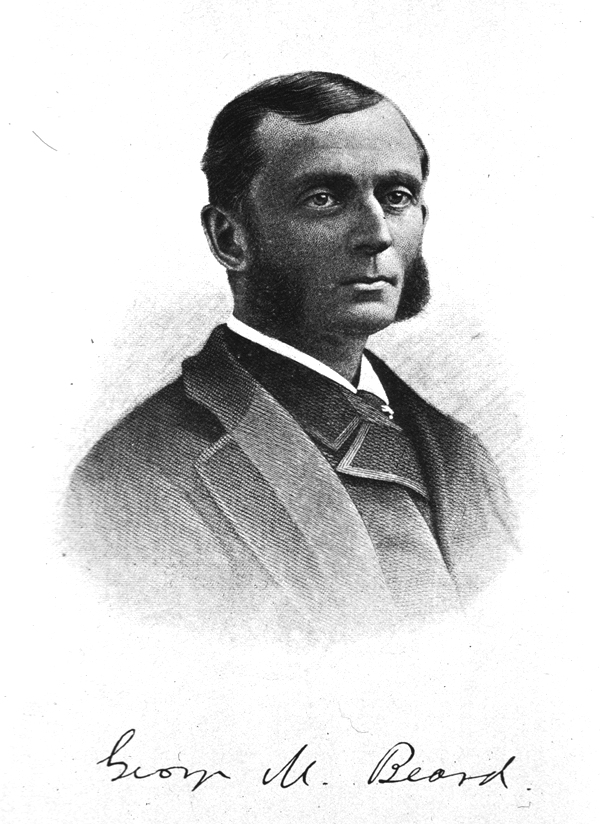
\includegraphics{George_Miller_Beard.jpg}\caption{George Miller Beard, See page for author [Public domain], via Wikimedia Commons}\label{fig:beard}\end{marginfigure}

Starting in the 1870s, Beard became increasingly interested in psychological disorders. In 1881, he published \emph{American Nervousness}, a book that came to define psychological treatment for a generation. `Nervousness' did not mean then what it means today: jitteriness or tension. Back then, it denoted a kind of fundamental exhaustion---what we still call a `nervous breakdown'. Technically, Beard defined it as:

\begin{quote}

``deficiency of lack of nerve-force. This condition, together with all the symptoms of diseases that are evolved from it, has developed mainly within the nineteenth century, and is especially frequent and severe in the Northern and Eastern portions of the United States. Nervousness, in the sense here used, is to be distinguished rigidly and systematically from simple excess of emotion and from organic disease.'' ~\citep[p. vi]{Beard:1881tg}
\end{quote}

American Nervousness was caused by ``modern civilization, which is distinguished from the ancient by these five characteristics: steam-power, the periodical press, the telegraph, the sciences, and the mental activity of women.'' ~\citep[p. vi]{Beard:1881tg}

Beard was building on both folk theory of innate energy as well as the recent discovery that nerves carried electricity, but he extended his view to cover diseases such as ``neurasthenia (nervous exhaustion{\ldots} hysteria, hay-fever, sick-headache, inebriety{\ldots} some and phases of insanity.'' ~\citep[p. vii]{Beard:1881tg} whose `signs' could include:

\begin{quote}

The nervous diathesis; susceptibility to stimulants and narcotics and various drugs, and consequent necessity of temperance; increase of the nervous diseases inebriety and neurasthenia (nervous exhaustion), hay-fever neuralgia, nervous dyspepsia, asthenopia and allied diseases and symptoms; early and rapid decay of teeth; premature baldness; sensitiveness to cold and heat; increase of diseases not exclusively nervous, as diabetes and certain forms of Bright's disease of the kidneys and chronic catarrhs; unprecedented beauty of American women; frequency of trance and muscle-reading; the strain of dentition, puberty and change of life; American oratory, humor speech and language; change in type of disease during the past half century, and the great intensity of animal life on this continent. ~\citep[p. vii-ix]{Beard:1881tg}
\end{quote}

Beard died shortly after the publication of \emph{American Nervousness}, but his cause was taken up by Silas Wier Mitchell (1829--1914), who popularized what became the standard treatment for American Nervousness: the ``rest cure.'' As you can probably imagine, if the cause of American Nervousness was modern civilization, including the recent suffragist movement, the cure was removal from modern civilization, including banning women from having a mental life.

\begin{marginfigure}\includegraphics{Perkins-Gilman.jpg}\caption{Charlotte Perkins Gilman, By Schlesinger Library, RIAS, Harvard University [No restrictions], via Wikimedia Commons}\label{fig:perkins-gilman}\end{marginfigure}In 1885, at the age of 25, Charlotte Perkins Gilman, a member of a prominent family of American progressives that included the abolitionist author Harriet Beecher Stowe, the suffragist Isabella Beecher Hooker, and the charismatic clergyman Henry Ward Beecher, gave birth to her only child Katharine Beecher Stetson.\footnote{We will encounter the Beecher family again in section \ref{forthefoundationsoftherace}.} After the birth, Charlotte Perkins-Gilman experienced what we now recognize as a severe case of post-partum depression.

She was taken to see Silas Wier Mitchell. She described her experience of the treatment she received this way:

\begin{quote}

``During about the third year of this trouble I went, in devout faith and some faint stir of hope, to a noted specialist in nervous diseases, the best known in the country. This wise man put me to bed and applied the rest-cure, to which all still-good physique responded so promptly that he concluded there was nothing much the matter with me, and sent me home with solemn advice to `live as domestic a life as far as possible,' to `have but two hours' intellectual life a day' and `never touch a pen, brush or pencil again' as long as I lived. This was in 1887.''~\citep{PerkinsGilman:1899ut}
\end{quote}

Her experiences you may know from the American Standard short story ``The Yellow Wallpaper'' (1892). Gilman acknowledged that she never suffered from the hallucinations her most famous character did, but that she ``came so near the borderline of mental ruin that I could see over.'' (1913)

While Doctors no longer prescribe isolation for women who want to be authors, we still use the basic idea of removal from society and `rest' for those who are mentally unwell. An `asylum,' after all, is a refuge, and most in-patient mental health institutions are branded as `restful' and located away from the pressures of contemporary life. 

\newthought{Back in 1887}, a German intellectual named Ferdinand Tönnies published a book which, in English, is usually titled ``Community and Society.'' It is considered, today, one of the foundational texts of sociology. In it, Tönnies distinguishes between the culture of the rural people (community) and the ``educated class'' (society). 

\begin{quote}

The common people are similar to women and children in that to them family life, along with neighboring and friendship, both of which are closely related to family life, is life in and of itself. Among the educated classes, is so far as they separate themselves from the common people and arrange their institutions quite independently{\ldots} These relations disappear more and more as the rational freedom of the individual comes to the fore. {\ldots} The life of the common people finds its fulfillment in home, village and town; the educated classes are urban, nations, international. (p. 168) 
\end{quote}

Whether Tönnies' characterization is true or not, there is a pronounced fear of losing one's culture if one becomes educated in many rural communities. 

Sherman Alexie, in his semi-autobiographical \emph{The Absolutely True Diary of a Part-Time Indian}, describes this fear by relating his thinking on his first day at a white school, Reardon:

\begin{quote}

Reardan was the opposite of the rez. It was the opposite of my family. It was the opposite of me. I didn't deserve to be there. I new it; all of those kids new it. Indians don't deserve shit.
\end{quote}

As his identity as an Indian had been cultivated in opposition to the White folks of Reardon, to enter Reardon was to negate everything he knew about himself. It was to betray his tribe and join `the other.' And it took an insane amount of bravery and self-confidence to even attempt it.

Alexie's experience bears similarities to John's, except that John was sent off to college as the best of his community, with their full support. It was only after he returned that he found himself alienated by his community. Alexie was alienated from his community in the act of seeking out education. 

A college education will---if it is done properly---change you. It will make you think differently about your life, your family, your values. It will make you aspire to things that you previously did not believe were possibilities. It will make you disagree with people who up until now you agreed with entirely. It will make you unhappy at times.

But, as Sherman Alexie says, joining a new tribe does not mean that you lose the old one. It means you have both, and that is a wonderful thing. Most ``tribal thinking,'' as Alexie calls it, is dangerous. Do not be afraid to think for yourself. If your ``tribe'' rejects you because you think for yourself, they never really accepted \emph{you} in the first place---they merely wanted another unthinking follower. 

Like with any healthy relationship---a friend, a lover, a spouse---if the other accepts you only the condition that you do not think for yourself, it is not a relationship between equals. Heck, it isn't a relationship at all. 

A friend is someone who wishes good things for you for your own sake, and not for any other reason, as Aristotle noted in the \emph{Nicomachean Ethics}.\footnote{The subject of much discussion in Chapter \ref{forcharacter}.} Education, when pursued for the benefit of the person educated, should be desired for any friend by any friend. Anything other than that raises serious moral questions.

\section{How to analyze a theory of education}
\label{howtoanalyzeatheoryofeducation}

Any theory of the value of a college education must, first of all, must specify an \nameref{thesis:educationalgoal}---the question with which we started this chapter. It must state the \nameref{purpose:educationalpurpose}. 
\begin{purpose}[The Purpose of Educating] \label{purpose:educationalpurpose} What is the purpose or goal of college education?\end{purpose}


In doing so, one must also define the \nameref{entities:entitieseducated} and the \nameref{objects:beneficiaries}. 
\begin{entities}[Entities educated - the subject of education]\label{entities:entitieseducated}Who are educated in an educational system?\end{entities}

\begin{objects}[Object or end of education] \label{objects:beneficiaries}Beneficiaries of the educational system.\end{objects}
 As we shall see in Part \ref{themanypurposesofhighered}, most colleges and universities articulate a mission, or a vision of themselves that makes reference to two or three purposes.

These mission and vision statements, which for many parents and students are little more than office decor, really do guide decisions at most institutions of higher learning. Courses, faculty and majors are evaluated on a regular cycle in connection with the assumed purpose of the institution. If you, as a student, have a particular view about the purpose of education, it is in your best interest to find a college or university that shares your view.

And that is the topic of this book.

\newthought{Stating an ideal} of an educated person is not the same as justifying why that ideal is desirable. Utopian fiction frequently presents a desirable future state to the reader, but does not argue \emph{why} that state is desireable---it just assumes that the reader will concur.

According to Diogenes Laeritus, Aristotle once claimed that the educated differ from the uneducated ``as much as the living from the dead,'' ~\citep[p. 463]{Laertius:eqeg5o3J} yet this does not, on its own, specify \emph{why} being educated is preferable, as it does not specify that being alive is preferable to being dead. Socrates, for example, questions this assumption in his \emph{Apology} directly. It may be thought obvious, as we can all assume that being alive is preferable to being dead, but, at the very least, it must made explicit, and the strength of analogy to being educated \emph{must} be made tested on exactly this point.

Again, most of the famous works we will consider in this text---such as \emph{The Republic} and \emph{Émile}---spend much of their time elucidating the ideal, with very little arguing for that ideal of education. Yet, in both cases, the argument for the ideal is really just a critique, often implicit, of the uneducated. For example, in \emph{The Republic}, the enlightened cave-dweller would ``would choose to endure anything rather than'' a life in the cave\footnote{\emph{The Republic}, and the allegory of the cave are the main topic of Chapter \ref{forstatecraft}.}.~\citep[516e]{Plato:1994ug} In \emph{Émile}\footnote{\emph{É⁠mile} is one of the central readings for Chapter \ref{forcharacter}.}, Rousseau repeatedly mentions the `civilized' or bourgeois man who ``is born and dies a slave'' ~\citep[p. 16]{Rousseau:2007vp} as an absurd conclusion of being uneducated in his system.

Our interest in this book is not just to create a taxonomy of educational goals, but also to elucidate and evaluate some of the reasons historically given for those goals.

\subsection{Evidence used in this book}
\label{evidenceusedinthisbook}

In this book, I am not immune from the criticisms of conflating value theory with empirical data. Over the course of the text, I highlight various educational theories in the great texts of the western tradition, and then trace those ideas into the modern era of higher education in the U.S. When I taught this class, I would assign each student or group of students a college or university that was well-known for adopting a particular theory of education. The students were to research the university, read the mission statement and curriculum, and present it to the rest of the class, highlighting where the relevant concept shaped policy---or at least, where it shaped the University's marketing material.

This book will do the same. In order to do so, I am not just reciting institutions that are `well-known', whatever that means. I rely on a corpus of documents harvested from colleges and universities during the writing of this book, starting in the summer of 2016. The corpus consists of about 426 0 home pages of colleges and universities, along with all their data publicly available through the Carnegie classification. Thus, when I say ``X University is the top university for focusing on Leadership in the Undergraduate curriculum'', I do not mean ``This is the one I've heard about the most'', but rather ``this university uses `leadership' and related terms more frequently in their corpus than any other college or university surveyed.''

All links on a University's main page that contained words like `about' or `curriculum'\footnote{The list includes: ``About'', ``At a Glance'', ``Mission'', ``Discover'', ``Mission Statement'', ``Purpose'', ``Who we are'', ``Overview'', ``Vision'', ``History'', ``Academics'', ``Program'', ``Curriculum'', ``Major'', ``Degree'', ``General Education'', ``Catalog'', ``President'', ``Academic'', ``Degree'', ``Advising'', ``Liberal'', ``Core'', ``Objectives'', ``Learning Goals''.} are harvested, and those pages subsequently crawled. Links on any `about' pages are also harvested, and any pages that were not already include are crawled. This gives us three `levels' of content: the main page, any secondary pages that are `about' or `curriculum', and any additional tertiary pages linked on the secondary pages.

The resultant corpus contains over 4260 main or primary pages and about 50,000 secondary-pages and 1,500 tertiary pages, or exactly 1 `main' page per college or university and about 11.35 sub-pages (average) per college or university. I update each institution in the corpus once every three months, so the dataset is constantly growing, and rankings and highlights may shift between publication and class offering. The most recent and up-to-date rankings, along with a per-college analysis and supporting documentation, is available at http:\slash \slash deliberately.college\slash . 

The resultant corpus provides evidence of how colleges and universities project their values to the outside world. It does not provide evidence of how those values are instantiated in, say, real-world matters such as budget decisions. But that is a different question, one that frequently roils the internal politics of an institution.

\subsection{Utopian thinking}
\label{utopianthinking}

\newthought{There is an analogy here to Utopian thinking.} Many Utopias are specified in the literature with little justification---the idea seems to be that the reader will just naturally see how this ordering of society is preferable to reality. And indeed, many writers about higher education just seem to assume that once you've tried it, you won't go back. Plato and Rousseau certainly do.\begin{question}
And so we return to our questions from the last chapter: is it possible to have an ideal educational system that produced individuals who knew---not suspected or believed, but actually knew---that their educational system was not perfect?  Does that not seem like a contradictory thesis?  An ideal system is, by definition, ideal, perfect, complete.  Therefore, any student to come out of that system with the acumen to think abstractly would necessarily come to recognize their systems' perfection---right? Does that mean that the presence of reasonable dissenters in an educational system entail that that educational system is, in fact, not ideal? And if so, doesn't that seem kind of totalitarian?

It seems certain that there could be a utopian society that contains reasonable differences of opinion regarding how that society should be shaped; but 'knowledge' requires not just that you believe something, but that it also be true. Can an educational utopia contain inconsistent facts about its own deficiencies and still be utopian?\end{question}

Moreover, specifying a purpose for higher education is meddling with social engineering. Higher education in our society is the final step in enculturation---it is the finishing school for the professional class. So specifying a goal for higher education is tantamount to specifying the characteristics of the professional class of a Utopian society.

One fruitful method of analyzing utopian thinking is to consider what the utopia in question is missing, when compared to our own society.\footnote{See, e.g. ~\citep{Carey:2000tt}, Introduction.} Thus, a racist utopia excludes those of different races. A `workers paradise' excludes the bourgeoisie. Charlotte Perkins Gilman's ``Herland'' contains no men, and as a result, she hypothesized, no domination and no wars. Religious afterlives exclude those of different faiths, offering the religious a fantasy of a monocultural religiously-cleansed world. 

Educational systems are often utopian fantasies that exclude the uneducated---but who, then, is that? When the William A. Sterns, then President of Amherst College, declared that the central principle of Amherst College ``is to make men,'' ~\citep{Stearns:1859vm} he was excluding not only women, but non-Christian men and those who were not \emph{real} men---i.e. any biological male who did not fit the model of masculinity and character in the Protestant colonial era. 

When Leo Strauss says that education is ``in culture or toward culture'', he excludes the uncultured.~\citep{Strauss:INKysbQ_} The 19th century advocates for mental discipline exclude the undisciplined. Dewey and followers who emphasize critical thinking exclude the unreflective or uncritical thinker. Religious educators exclude the irreligious, and so on.

When educators sit down to think about what their college should do---from orientation to graduation---they working through utopian visions of an educated society. And just analyzing that which a utopia leaves \emph{out} can be a fruitful exercise, analyzing the faults an educational theorist seeks to correct can shed new light on educational philosophy long since adopted.

\section{Conclusion}
\label{conclusion}

Adequate specification of an theory of higher education requires specification of both the entities educated (the subject of education) and the beneficiaries (the object of education). Doing so is a philosophical value-based claim, which is logically prior to the empirical task of determining precisely \emph{how} an educational practice will lead to those objects. 

The `crisis' of higher education today masks a fundamental disagreement about the role a college or university is to play in our society---i.e. for whose benefit a higher education is pursued. 

In this book, we will consider a number of different theories of education that are instantiated in the structures of higher education in the US today. These theories are given voice by some of the `great works' of the Western Tradition. Our goal is not to understand these works on their own, but rather to understand how they informed the construction of the institutions that we now inhabit. 

To make the connections between the old and the contemporary, we rely upon a corpus of the websites of all existing English-speaking college and universities in the US, along with our analytic technique borrowed from the study of utopian fiction of considering the individuals excluded from an educated society.

\part{The many purposes of higher ed}
\label{themanypurposesofhighered}

\chapter{For vocation}
\label{forvocation}

\marginnote{\emph{We must guard against the temptation to think that a man's worth as an individual or his value to society can be measured by his aptitude for mathematics or languages. We must recognize that there are diversities of gifts, but whether it be plumbing or Plato that is in question, a society that is not to be condemned to mediocrity must demand the best of each.} -Frank Aydelotte, \emph{Breaking the Academic Lockstep} (1944)}

In 1800, the Swiss-Italian teacher Johann Heinrich Pestalozzi and his young teaching assistant Hermann Krüsi, started a school at Burgdof castle near Bern, Switzerland. It closed just 4 years later, in 1804. 

Pestalozzi and Krüsi did not succumb to their failure and give up. They redoubled their efforts, and in 1805 started another school at Yverdon, which grew into an internationally renowned institute and is now widely seen as the origination of elementary education. Pestalozzi's ideas inspired Maria Montessori, John Dewey and a large number of other educational reformers. 

In 1820, Pestalozzi published a new edition of the educational work he wrote at Burgdof called \emph{How Gertrude teaches her children.} In the preface, he recounts the failure of the Burgdof institute in this way:

\begin{quote}

Matters strange and far removed from our duty soon absorbed our time and powers, and gave a mortal blow to the simplicity, the progress, the concentration, and even the humanity of our original efforts. Great ideas for improving the world, which arose out of elevated views of our subject, and which soon became exaggerated, filled our heads, confused our hearts, and made our hands careless of the needs of the Institute that lay before our eyes.~\citep[p. 3]{Pestalozzi:1894vz} 
\end{quote}

\begin{figure*}\includegraphics[height=10cm]
{Birr-Grab-Pestalozzi-3.jpg}\caption{Mural above Pestalozzi's tomb, Public domain, available on wikimedia commons. Notice the two boys on the left, presumably already his pupils, at work planting a tree.}\end{figure*}

His explanation of his failure from \emph{Gertrude} demonstrates a first-rate thinker engaged in candid self-appraisal. For Pestalozzi, the educated person balanced the intellectual, moral, and practical capacities of humankind---what he calls herein the `head', the `heart', and the `hands.' This is the criteria upon which he judges his students, and the goal for which his educational system was designed.

In this quote, Pestalozzi has applied the metric by which he measures his students to himself, and found himself wanting. The `great ideas', which, in passive voice, `arose out of elevated views of our subject' and `became exaggerated', distracted his intellect from the tasks of maintaining morality and attending to the practical realities of running an institute.

Here we have a highly educated individual who has dedicated his live to education. Yet in his own estimation, he failed, not because of his lack of ideas, or because of some insurmountable outside force, but precisely \emph{because} his ideas were too grand. Wait, What?

We are frequently told that American innovation is the key to economic growth. We are told that the best amount us become entrepreneurs with 'big ideas. Or that `true leaders' have grand visions of the future. Why would Pestalozzi explain his failure on his `grand ideas'?

The passage quoted suggests that success requires not just new and novel ideas, it requires new and novel ideas that are tempered against the practicalities of the actual problems that ``lay before our eyes.'' 

According to Pestalozzi, knowledge comes from five sources: 

\begin{enumerate}
\item `accidental' or random experiences, which produces `irregular' or `confused' ideas.

\item experiences guided by our teachers or parents, which produces, when done correctly, clear ideas.

\item From the will and the desire to obtain ``notions, knowledge and ability'', which gives `intrinsic value' ideas and ``brings us nearer to moral self-active education.''

\item through effort or work, which connects ideas to reality,

\item by analogy, which compares ideas and connected them together, allowing for abstraction. 

\end{enumerate}

1,2,3 and 5 are completely consistent with the theories of psychology that were standard at the time: all ideas originate in sense-impressions; and abstract ideas originate in comparisons between sense-impressions. Recall from section \ref{structureofeducationaltheory} that the 18th and 19th century empiricists modeled the mind as a tabula rasa, where the objects of sensation `impressed' themselves onto the block of wax. This is true of Hobbes, Locke, Hume, Berkeley, etc.---they all agree, in broad outline, with numbers 1,2,3 and 5.

Pestalozzi's number 4---work---is interesting and novel when viewed against this background setting. In \#4, knowledge comes:

\begin{quote}

From the results of effort, work \emph{at one's calling}, and all kinds of \emph{activity}, the object of which is not merely sense-impression. This manner of gaining knowledge connects my sense-impressions with my \emph{conditions and position}, and brings the results \emph{into harmony with my efforts} towards \emph{duty and virtue}. It has, through the necessity of its course, as well as through its results, the most important influence on the \emph{accuracy, continuity, and harmony} of my insight, as well as on the purpose aimed at making ideas clear. ~\citep[p. 115, italics mine]{Pestalozzi:1894vz} 
\end{quote}

I have highlighted a number of sections in this passage. First, Pestalozzi does not talk about just any work, but rather `work at one's calling'---one's `vocation.' Work is important, but not just any mindless labor. For work to be educative, it must be work at one's vocation, or `calling'.

Second, action, not just thinking, connects the ideas in one's head to one's ``conditions and position'', bringing the ``results into harmony with my efforts.'' For the empiricists, there are \emph{no} ideas that are not ultimately based in sense-impressions. This statement is, in part, the fundamental belief of the empirical tradition. Yet Pestalozzi has said here that this knowledge is \emph{not} based in sense-impression!\marginnote{Recall that Pestalozzi's diagnosis of his failure in Burgdof was precisely this: his ideas became disconnected from the practical realities in front of him.} But Pestalozzi is not a dualist, arguing for innate ideas or ideas that must come from the non-physical world. He is adding \emph{actions}, not just sense-impressions, to the list of things that can produce ideas.

Third, work is not random. It is directed towards `duty and virtue'---that is, work develops the moral character of the individual. If this were in the modern language of educational outcomes, the `goal' would be the development of the moral character of the individual, while the `outcome' would be the improvement in the `harmony' of thought with action.

And, finally, work has a tangible impact on the intellect, improving the ``accuracy, continuity and harmony'' and clarity of thinking. Again, to make this explicit---contrary to the views of Hobbes, Locke and Hume---clarity of thinking is cultivated by \emph{action}, not just sense-impression.

This brings us to the first major thesis of educating for vocation: in Pestalozzi's thinking, by refining our ideas, work training benefits the students themselves.\begin{objects}[Pestalozzi's Beneficiaries]
\label{pestalozziobjects}The beneficiary of education is the the students themselves through the unique development of character and the intellect that is accessible *only* through first-person action.
\end{objects}


As we shall see, not every vocational theories agrees with \ref{postalozziobjects}.

\section{Plato: The Thesis of Specialization}
\label{plato:thethesisofspecialization}

At the very beginning of Plato's \emph{Republic}, one of the foundational texts of western Philosophy can central text for Chapter \ref{forstatecraft}, Socrates asks the question ``What is justice?'' His first two interlocutors, Cephalus and Thrasymachus, propose solutions that are easily dispatched by Socrates. While these are interesting and important discussions, they are not directly relevant to the question of education, so we will skip over them here.
\begin{thesis}[Thesis of Specialization] \label{eq:specialization}
The best possible work can be gotten from an individual if and only if that individual is naturally suited to this work, and the individual is trained solely and exclusively for that work.\end{thesis}

Once Thrasymachus has left the dialogue, Socrates settles into discourse with the main two interlocutors of \emph{The Republic}, Glaucon and Adeimantus. At the end of Book I and the beginning of Book II, they determine to investigate the idea of justice by engaging in a thought-experiment. Starting from nothing, they intend to create an ideal just city-state, a Utopia, so that they may ``See justice in the large{\ldots}'' On the assumption that the character of a state will reflect its inhabitants, and vice-versa, an ideal, utopian city-state will reflect the ideal, utopian individual.

To start out, all the participants in the discussion quickly agree that ``one man is naturally fitted for one task, and another for another'' and that ``one man would do better work if he did not work at many tasks, but stayed at just one.'' (370B)

Neither Adeimantus or Glaucon gives an argument in response to Socrates' assertion. They simply accept this as a fact and continue on. As we shall see, the utopian system that they will develop in the following books of \emph{The Republic} rely crucially on the presupposition that: ``one at one'' is the best way of working.

To make it explicit, we will call this claim the ``\nameref{eq:specialization} (Thesis \fullref{eq:specialization}).''

The \nameref{eq:specialization} is neither argued for or defended directly. It must therefore be a utopian assumption---a kind of working hypothesis whose adequacy is judged by the adequacy of the system created from it. 

If the utopian society created on the basis of the \nameref{eq:specialization} works, it would give us reason to believe the \nameref{eq:specialization} is true---or, at least, useful. And if it does not work, then there is reason to think the \nameref{eq:specialization} is false. 

Just as utopian thinking can be analyzed by looking at what is left \emph{out} of the utopian society, we can analyze Plato's ideal city by looking at what Socrates, Glaucon and Adimanteus have left out. \nameref{eq:specialization} excludes those who wish to do---or attempt to do---things for which they are not well suited, or have not been specifically trained.

Thus, when Socrates introduces the need for a standing army to his ideal city, he relies on the \nameref{eq:specialization} to ensure that members of the army are trained specifically and solely for fighting:

\begin{quote}

``We surely agreed, if you remember, that it is impossible for one man to do the work of many arts well.
True, he said.
Well, then, said I, don't you think that the business of fighting is an art and a profession?'' (374B)
\end{quote}

Further examples will follow in Chapter \ref{forstatecraft}.

When people discuss Plato's theory of education, they usually mean the educational system he designs for the rulers of his ideal city, which we will discuss in depth in section \ref{forleadership}. But it is important to remember that all of that is based on the assumption of \nameref{eq:specialization}. Everyone in Plato's ideal city is trained solely and completely for his or her \emph{vocation,} to which they are destined from an early age. 

\newthought{While I will not bother defending} Plato's utopian vision as a desirable state of affairs, I do believe it is important to recognize the impact his thinking has had on the development of our institutions. Economic advancement in the modern world has been fueled largely by specialization---Adam Smith argued that the division of labor was key to developing the 'wealth of nations, while Karl Marx postulated that the division of labor was the root of alienation in modern laborers.

Contemporary institutions---including corporations---largely follow Plato's ideal. Tasks are broken up into increasingly specialized parts, and while at work, individuals are expected to specialize in their particular job. In many cases, the specialization means that one cannot advance to a new position without changing institutions, as specialization can mean getting stuck in a pidgeon-hole. Yet CEOs and senior executives are meant to be well-rounded, and have multiple competencies across the needs of their organization.

\section{For Whom?}
\label{forwhom}

\marginnote{\emph{"What is needed here is an education for the head, hand and heart"} - Samuel Chapman Armstrong, quoted in ~\citep{Spivey:1978un}}

In his 1978 book \emph{Schooling for the new Slavery: Black Industrial Education 1868--1915}, Donald Spivey argues that ``Industrial education was a major force in the subjugation of black labor in the New South.'' ~\citep[P. IX]{Spivey:1978un}. Yet today, half of the Americans surveyed said that the main purpose of College was to teach specific skills needed in the workplace. ~\citep{PewResearchCenter:2016ut} 

There is little question that racists in the Reconstruction South, including Samuel Chapman Armstrong, used practical and vocational education to direct the aspirations of freed slaves into service positions; yet today we see small liberal arts colleges, such as Stirling College,\footnote{Stirling College, whose motto is 'Working hands, working minds, is located in Craftsbury Common, VT, which is 96.74\% white---about as far from Tuskegee, Alabama demographically as we might get.} return to practical and vocational education.

In 1999, the Lilly foundation launched an Endowment project for the Theological Exploration of Vocation. It has funded programs at religiously-affiliated small liberal arts colleges, a category of college that was once defined in direct opposition to vocational education. Catholic institutions in the US continue their commitment to liberal arts education, yet Joseph J Dunn wrote in the journal `America: The National Catholic Review', that traditional liberal arts colleges ought to teach its students to ``understand the language and functions of business, and its role in society.'' ~\citep{Dunn:2016vz}

In fact, the 1940 US Census, which was the first to ask residents about their highest level of educational attainment, did not count 'private schools for art, music, drama, etc., private trade and vocational or private correspondence schools" ~\citep[p. 118]{Harriman:1947wh} as qualifying `education.'

How do we make sense of all of this? How can it be simultaneously true that elite small liberal arts colleges are developing vocational programs, sometimes with support from major endowments; and at the same time, vocational education has been used to reinforce the stratified society that prevented the laboring class from enrolling in elite colleges and universities in the first place? 

\newthought{As we noted in} \S\ref{structureofeducationaltheory}, an adequate theory of education needs to specify both the entities educated and the entities who benefit from that education.

The question at hand can be resolved by attending to this distinction. An educational system that truly benefits the student will do so whether it is vocational or avocational. And an educational system that is designed to keep certain individuals in subservient roles, for the benefit of those served, would be immoral regardless if it were vocational or avocational. 

But it does seem easier to conceive of a vocational educational system designed to enforce hierarchy than an avocational one. Hierarchical societies depend on strict enforcement of societal roles. Vocational education tends to train individuals specifically for societal roles. If vocational education is set up to train individuals \emph{exclusively} for societal roles, like Plato's, it threatens to descend into totalitarianism. 

In his 1912 speech `Vocational Education' Senator Carroll S. Page called for the teaching of vocational subjects in state normal schools. He closes his argument with these sweeping insights:, 

\begin{quote}

The American People want, most of all, occupation, and at wages which will give them bread and enable them to give their children an education that will equip them for the struggles in life. Mr. President, we must not do injustice to the laboring man{\ldots}see that his children have the opportunity to receive and education, and that kind of education too, which shall fit and equip him to be self-respecting and self-supporting{\ldots}Mr. President, the occupied man is a good citizen. It is easy for the agitator to call the idle man to deeds of violence and anarchy{\ldots} ~\citep[P. 66]{Page:1912we}
\end{quote}

The Congress did, in fact, produce the Smith-Hughes Vocational Education Act in 1917, which provided such funding to the states. Page argues that vocational education makes the student `self-respecting and self-supporting' as well as `a good citizen.' The first of these---`self-respecting and self-supporting'---makes the beneficiary of education as the student; while the second---a `good citizen'---implies, at least, that the beneficiary of vocational education is the continuation of the existing social order. Education for good salaries but not social importance may suffer from the same criticism.

Spivey's critique of black industrial education\footnote{The ``National Society for the Promotion of Industrial Education'' was a lobbying group founded in 1906 in support of proposals like Page's. It gave way, starting in 1910, to the ``National society for vocational education'', which combined with ``Vocational Education Association of the Mid West'' to become the ``American Vocational Association'' in 1926.} in the New South is exactly this: that it taught exclusion and hierarchy, not for the benefit of the individuals, but for the benefit of the existing social structure. While this may be the case, this critique clearly misses the mark when applied to other advocates for the education of the `hand', including Pestalozzi.

\subsection{Why Work?}
\label{whywork}

Ask students today why they are in college, and most will respond `to get a job.' This, I am certain, is a superficial response. Probe it a little: why this job? Why must you go to college to get it? Why this college instead of the many others that can provide the requisite certification?, and you will pretty quickly discover just how shallow the `job' response is.

For Pestalozzi, the economic value of a particular kind of work is far less importance---indeed, it is not even mentioned in the text---than the intellectual and moral benefits of work. Work experience provides a kind of knowledge that is unavailable otherwise. It requires that you put your ideas into actual actions, and evaluate those ideas in the hard light of reality.

I can have an idea for the greatest computer game in history, but without some basic coding skill, I would not know how to write something that could run within the memory and processing constraints of the target console. If I aspired to architecture, I could design grand structures that soar to the heavens, but without knowledge of the load limits of the materials used, the structure would never stand. 

The real world has a way of resisting our imaginings that constrains and disciplines our thought processes. Try as I might, I cannot, without intervening in the world physically, by sheer force of will, make a parched plant moist. 

Run up a flight of stairs---at that moment when you take the accidental `extra' step and humiliate yourself, you believed entirely, top to bottom, heart and soul, that there was an extra step. But there wasn't. No amount of mental force will make that extra step hold your foot.

\begin{marginfigure}\includegraphics{Sandrogiodano-MY-LOVELY-BOY.jpg}\caption{"My Lovely Boy", by Sandro Giodano. Sandro Giodano is an Italian artist whose photos show individuals at the moment where their world is "falling-down." His work, and his artist statement, can be browsed at http://www.sandrogiodanoinextremis.it/. NEED PERMISSION}\label{fig:giodano}\end{marginfigure} The internet is, as you probably know, filled with videos of people whose expectations for how the world behaves were inconsistent with the reality. I'll leave it to you to investigate.

\subsection{Liberal v. Vocational Education}
\label{liberalv.vocationaleducation}

There is no doubt that career-focused institutions and majors are popular in today's economy. But I suspect that today's economic realities are only part of the explanation. It is true now, just as it has always been, that a college education increases one's economic prospects. 

Those who lament the glory days of the liberal arts education in America forget that a training in letters---especially those heavy on the classics---was necessary for careers as preachers and teachers, lawyers and politicians. Indeed, Abraham Lincoln famously practiced law with almost no formal education at all. W.E.B DuBois taught elementary school without studying education. Even John Locke, the great English Philosopher, was a tutor to the young Lord Shaftesbury.

Harvard was founded, famously, for the training of a clergy for the new world, and Yale's charter specifically mentions careers.\footnote{\begin{quote}

``wherein Youth may be instructed in the Arts and Sciences (and) through the blessing of Almighty God may be fitted for Publick employment both in Church and Civil State.''
\end{quote}} Brown, Rutgers, Dartmouth and Princeton were all founded as part of The Great Awakening, out of frustration with Harvard and Yale's production of clergy not on board with this new form of Christianity. 

While it may still be technically possible to become a lawyer and join the bar today without attending law school, it is exceedingly rare. And there are certainly are no great opportunities for economic stability for the `man of letters' today outside, perhaps, of the clergy and research--1 universities. 

There never was a ``golden age'' when American liberal arts education existed free from the concerns of vocation. To pretend otherwise is as ignorant as those revisionists who romanticize the antebellum South. What is true is that there have been periods of time when one could find a vocation with a sharp mind and without practical training. But those are rare, and with growing specialization in an advanced economy, increasingly so.

It is also true that within the rich tapestry of American colleges and universities one can find pockets of independently wealthy students who are, individually, free from the concerns of vocation. And in many colleges, there are at least a handful of students who have guaranteed positions in their family business after college, and as a result, feel themselves unconstrained by economic pressure. But no institution---not even an Ivy---exists solely to serve such students.\footnote{In January 2017, The New York Times published a study comparing the number of 1\% students served by the institution against the number served from the bottom 65\%. Washington University in St. Louis, not Harvard, took the top spot. See ~\citep{Aisch:2017wg} for full detail.} Contemporary institutions are, by necessity as well as tradition, designed to educate for character, culture \emph{and} career. The myth of the liberal arts education free from career concerns comes from an era when character and culture were sufficient, on their own, to make a career. That era has passed.

\begin{marginfigure}\includegraphics{Netscape_Navigator_122_Screenshot.jpg}\caption{Screenshot of Netscape Navigator 1.22, which was the first 'main-stream' web browser.  Screenshot from wikimedia commons By Indolering (Own work) [CC0], via Wikimedia Commons}\label{fig:netscape}\end{marginfigure} \newthought{Please allow me a quick digression} by way of personal anecdote. I graduated undergraduate in December of 1995---6 months after Netscape, the first commercial web browser, went public. I had the good fortune of having worked my work-study job in computer support; and being the low man on the totem pole because I was a Philosophy major and not a Computer Science or Math major, I was given the task of setting up my college's first website. The `cool kids' worked on Gopher and Archie. 

In 1995, it was possible to have a little knowledge and a liberal education and start a career in web design and production. And that's what I did. I eventually moved over to UNIX system administration and had a pretty good career, until the tech bubble burst and I went to graduate school. 

I mention this because during this boom time---a time that then Chair of the Federal Reserve Alan Greenspan called `irrational exuberance'---one could get a job with a well-rounded education and a taste for precision in language. 

But these times are rare. And even when the exist, most individuals in the bubble come out with little to show for it. For every Peter Theil and Elon Musk\footnote{Now billionaires, Theil and Musk started PayPal in the 1990s, before it was acquired by eBay.}, there were thousands of coders and system administrations who just didn't get the right funding, or weren't as cut-throat, or who simply lacked business savvy. We were the Steve Wozniaks\footnote{Steve Wozniak was the engineer behind Apple in the early days. He retains the status of a folk-hero in much of the internet and electrical engineering world.} of the world, and unlike Woz, we either didn't have a charismatic charlatan like Steve Jobs, or if we did, we were not able to tolerate them long enough to cash in.

While it is possible to find pockets of independently wealthy students unconcerned by the pressure of economics, we cannot structure our institutions on the assumption that these economic free-for-alls exist, and these kinds of opportunities are available at all times, to all students. Entrepreneurialism is great, but the moments of opportunity when entrepreneurialism reigns are fleeting. Institutions must serve all their students, not just the few who are lucky enough to graduate at a moment of irrational exuberance.

\section{For Head, Heart and Hands}
\label{forheadheartandhands}

In 1762, Jean-Jacques Rousseau, the Philosopher most closely associated with the French Revolution, published his treatise on Education titled \emph{Émile}. While we will consider \emph{Émile} in depth in Chapter \ref{forcharacter}, it is important that we note him here in order to trace the development of the idea of educating for vocation.

Rousseau's \emph{Émile} presents an imaginary case of a young boy who Rousseau raises from infancy to his introduction to high society as a young man. The 1760's were a period of opulence and decadence in the royal courts of Paris and Versailles. The wealthy, whether aristocrats or the newly rich business-class (now called `bourgeoisie'), aspired for their children to experience the finery and delicacies of the Court. Education, then, must be in those manners and customs of the `gentleman'\footnote{Recall from section \ref{themannerofeducation}, that the `liberal' in `liberal education' refers to the freedom of the men who pursued this kind of education. Free men were, at this time, those not bound to a Lord or craft, i.e. the `idle rich' or `gentleman.'}---knowledge of latin and greek, appreciation of the art forms favored by the Royals, sensitivity to social decorum and proper pronunciation.

\begin{marginfigure}\includegraphics{DOI_Rousseau.jpg}\caption[Frontispiece from Rousseau's *Discourse on Inequality*]{Frontispiece from Rousseau's `Discourse on Inequality'. The title is ``He returns to his equals.'' In his book on Rousseau and the paintings of Marsden Hartley, Joseph R. Reisert explains the context of the image thus: ``The Governor of the Dutch colony at the Cap of Good Hope had reared from infancy a child taken from among the natives. The youth had received a find education and had sufficiently impressed his patron that he was sent to work in a position of some responsibility., Having chanced to visit some o f his native relatives, however, the young man abandoned his civilized existence, choosing instead to live among the savages. To Rousseau, the importance of this incident lay in this: the Europeanized savage was in the rare position of being able to appreciate the advantages of both ways of life, and, from this epistemically privileged position, he rejected civilization.'' ~\citep[P. 31]{Reisert:2003tw} NEED HIGH-RESOLUTION SCAN}\label{fig:rousseau}\end{marginfigure}Rousseau rejected all of this. He opens \emph{Émile} with the unequivocal declaration that:

\begin{quote}

``Everything is good as it comes from the hands of the Author of Nature; but everything degenerates in the hands of man.'' 
\end{quote}

Rather than learning to appreciate the `finer things', Rousseau's imaginary pupil Émile would be taken daily to the `open meadow' ~\citep[p. 43]{Rousseau:2007vp} where he will experience nature directly, be hardened thereby, and learn to depend on himself. 

Rousseau wrote at time where the gilt and lavish lifestyle of Paris is contrasted by the French `encounter' with the native peoples of North America. Whereas the well-to-do in Paris could tolerate only the smallest fluctuations in temperature, Native Americans were thriving with little clothing or protection against the weather. Whereas the Parisians depended entirely on a vast network of food production and transportation to feed themselves, the Native Americans were robustly self-sufficient. 

For Rousseau, then, the Native Americans are `good,' insofar as they are `from Nature,' and Parisian society is `degenerate', having corrupted the pure `natural man' to the foppish dandy of high society. Recall John Stuart Mill's argument which we considered in Chapter \ref{introduction} that for those who had experienced both the pleasures of being educated and the `base' pleasures of the flesh unanimously preferred the `higher' pleasures to the `lower.' Rousseau flips the argument on its headnby claiming that having experienced the pleasures of the Court, he would prefer those of the peasants.

This is what we today call the myth of the `noble savage,' and it is surprisingly common in contemporary thinking. It teaches that civilization is the cause of all evil, and the uncivilized live correctly---whether that be defined as `peacefully,' `sustainably,' `in harmony with nature,' or, in Rousseau's thinking, `in a state of perfect equality.' The cure to society's evils is, therefore, a return---as much as is possible---to the pre-civilized way of life. We will return to Rousseau and this idea in depth in \S\ref{formanliness}.

\newthought{Pestalozzi is by no means} the only thinker of this era to be inspired by Rousseau's romantic portrayal of the peasant way of life and his call to get `back to nature.' But unlike Rousseau's unequivocal enthusiasm for the natural world, Pestalozzi's thinking was tempered by real experience.

In Pestalozzi's thinking, the education of an individual student ought to be a microcosm, or shortened reconstruction of how the species\footnote{The standard translations here say `race', meaning `human race', but in modern readings, it sounds awkward and suspicious. I have no idea if Pestalozzi was, himself, a believer in biological determination of intellectual and moral attributes according to racial categories or not. Nor do I care---unless it can be shown that there is something in the view that is unreconcilable with our present-day knowledge of failure of biological determinism. And I don't believe there is.} developed. In other words, Pestalozzi, following Rousseau, argued that the starting point for elementary education ought to be Nature. But unlike Rousseau, Pestalozzi holds that Nature is not perfect. It has a certain capriciousness with respect to any single individual that must be accounted for. 

\begin{marginfigure}\includegraphics{Victor_of_Aveyron.jpg}\caption{Cover of the book 'Victor of Averyron', Public Domain, available on Wikimedia commons.}\label{fig:aveyron}\end{marginfigure}In 1799 and 1800, almost 40 years after the publication of \emph{Émile}, the people of Aveyron in the south of France started reporting the existence of a `wild boy'. The idea of a child raised entirely in nature resonated with the French thinking in that moment, at the end of the French Revolution. Here was a real Émile: a child raised outside of society, without the damaging effects of the society they had just reformed: the wild boy of Aveyron.\footnote{For a review, see ~\citep{Lane:1979wq}. The original case book by Itard is republished in 1932 as ~\citep{Itard:1932wq}} WHAT HAPPENED 

Rather than romaticize the wild boy as free from the moral failings of society, Pestalozzi recognizes that nature is cruel. It does not care if one individual lives or dies, it only `cares' about the species as a whole. Individuals can be endangered, or even killed, if it is better for the whole. In modeling nature, teachers should never endanger their children; so the task of the educator is to attend to the development of the species, find the patterns encoded therein, break down those patterns into individual tasks, which can be safeguarded for individuals, and arrange them in a way that will step the individual through a quickened `natural' process of development. 

Writing is taught by first showing the students basic lines, angles and shapes, while naming them, and then encouraging the students to draw the shapes by themselves. These lines and angles are then cut up and recombined in to letters, and again, the child is encouraged to draw them on their own. Arithmetic is taught by putting together and separating various objects, asking the students to do the same, and instructing all along. The job of teaching, then, is to break down a complicated task into its component parts, and instruct those parts in graduated series of exercises, based on simple observation and participation.\footnote{For example: 

\begin{quote}

We want a graduated series of exercises, from their simplest beginning to their highest perfection, that is, to the utmost delicacy of nerve power, which enables us to perform with certainty and in a hundred different ways, the actions of thrusting and parrying, swinging and throwing. We want, too, actions exercising hand and foot in opposite, as well as in the same directions'. ~\citep[p. 178]{Pestalozzi:1894vz}
\end{quote}} 

According to Pestalozzi:

\begin{quote}

Nature needed ages to raise our race to perfect power of speech, yet we learn this art, for which Nature needed ages, in a few months. [In teaching our children to speak] we follow exactly the same course that Nature followed with the human race. We dare not do otherwise. And she unquestionably began with sense-impression. ~\citep[p. 149--150]{Pestalozzi:1894vz}
\end{quote}

\begin{purpose}[For Vocation-Pestalozzi:]\label{def:forvocation-pestalozzi}
Educating for vocation takes as its goal the growth of knowledge to the individual, and is required because this kind of knowledge can only come through physical action.
\end{purpose}

Recall that Pestalozzi believes that action---work---provides a kind of understanding that is unavailable through the other senses. In learning to speak, young children do not sit passively and listen. They babble, mimicking and imitating the sounds they hear around them. Thus, to truly learn how to speak, children must \emph{act}. Action provides feedback to the understanding and `tunes' it to the particular situation. Without action, understanding is incomplete.

Just like the subjects of Giodono's photographs, the world constrains our ideas about it through feedback on our actions---work---not mere speculation. Pestalozzi's notion of the importance of work weaves a thread through the history of vocational education in the European tradition, but it is sometimes difficult to discern. 

The most famous advocate of vocational education in the history of the United States is, without question, Booker T. Washington of the Tuskegee institute. To understand his thinking, and the differences between his conception of vocational education and Pestalozzi's, we have to step carefully through the development of the social sciences themselves.

\newthought{Auguste Comte, who we credit with the foundation of the social sciences,} was born to a wealthy family in France in 1798 --- immediately after the bloody revolution to a family of monarchists---a very unpleasant position hold in 1798.
\begin{marginfigure}\includegraphics{Comte.jpg}\caption{The bust of Auguste Comte, from Chapelle d'Humanitie (the Humanist's chapel). By Jean-Pierre Dalbéra [CC BY 2.0 (http://creativecommons.org/licenses/by/2.0)], via Wikimedia Commons}\end{marginfigure}
Comte was educated in the traditional French way, learning latin and greek and reading all the classics. When he was 14, he rejected his upbringing and set his mind of science. While he was ultimately admitted to the \emph{École Polytechnique} in Paris, legend has it that his application was initially denied, despite the fact he had the highest score on the entrance exam, simply because he was so young. Incidentally, he was expelled, along with his entire class, two years later in 1816 for `radicalism.'

Comte published his \emph{Cours de philosophie positive} in 1830, excerpts of which are published in English as \emph{Introduction to Positive Philosophy.}\footnote{All quotes herein are to the Hackett edition of this work.} Comte's ``positive'' philosophy held that every form of human knowledge passes through three developmental stages: the theological, the metaphysical, and the scientific, or `positive.' Francis Bacon, who we will discuss in \ref{originindemocraticepistemology}, initiated the scientific era for the physical world---i.e., what we now know as physics and chemistry. Comte believed that 1800 was the time for the study of humans to take the next step and become scientific---i.e., become what we would now call ``sociology'' and ``psychology.'' 

If this is to happen, positive philosophy must produce, first of all, the 

\begin{quote}

laws that our intellectual functions follow in their operations and, consequently, a precise knowledge of the general rules that are suitable for our guidance in the investigation of truth.`` [p. 24] And second, as a consequence thereof, positive philosophy must engage in a ''general recasting of our educational system. ~\citep[p. 24]{Comte:sZv664Ah}
\end{quote}

For Comte, and his followers, education was a logical outcome of the study of the human mind; and should, therefore, be studied with the same scientific methods of any other discipline.

\newthought{Herbert Spencer}---who was the probably the most famous english-speaking philosopher of his time---was a devotee of Pestalozzi's method.\footnote{See, e.g. ~\citep[p. 69]{Spencer:1861ts} and p.110--130 for Spencer's review and critique of Pestalozzi's theory.} So much so that his 1861 book \emph{Education} had three parts: Intellectual, Moral and Physical, or `head, heart and hands.'
\begin{marginfigure}\includegraphics{Herbert_Spencer.jpg}\caption{Herbert Spencer in 1889. Photograph [CC BY 4.0 (http://creativecommons.org/licenses/by/4.0)], via Wikimedia Commons.}\label{fig:spencer}\end{marginfigure}Spencer's approach was distinctly `positive', as he sought to apply the laws of biology to understanding human psychology, sociology, and hence, education. We call this view, today, ``Social Darwinism.'' 

``Social Darwinism'' has been used to justify all sorts of evils, including eugenics, colonialism, racism and genocide. As a result, the view, or anything like it, tends to produce revulsion in the modern mind. But that does not mean that there are not still some traces of Spencer's ideas alive and well in the structure of education institutions today. As is the case for all thinkers we cover, I am not attempting to rehabilitate Spencer, only to explain where and how his ideas became a part of the institutions we inhabit. But to do so, I need to present these ideas sympathetically, to show why intelligent and caring people in the past believed what we now consider nonsense.

For Spencer, who coined the phrase `survival of the fittest,' the first step in designing an educational system is to determine the relative value of different subjects of study. This should be familiar concept---anyone who has tried of choose a major or schedule classes knows well that choosing one subject often precludes the possibility of studying another. Spencer's challenge is to determine the way in which the `value' of different subjects can be measured.

Faculty at Montevello University in Alabama have engaged in a `liferaft' debate annually for the last 19 years. In this debate, disciplines are pitted against one another to determine which discipline is the most important---which single discipline would one take on a liferaft, if there was room for only one. Mathematics has won three times, History and Biology twice, Philosophy, Theater, English, Sociology, Culinary Arts, the university President, Political Science, Medieval Literature and Physics have all won once. The `Devil's Advocate', who argues against all the disciplines, has won twice. 

Spencer would love this. By putting disciplines into direct competition for scarce resources, we are imposing the Darwinian selective pressure on the academy. What we need, he would point out, is the criteria upon which we would decide who was the winner and who the loser. In biological evolution, the criteria for `winning' is passing on one's genes. At Montevello, it is getting the most votes from the assembled students. In education, Spencer argues: 

\begin{quote}

happily, respecting the true measure of a value, as expressed in general terms, there can be no dispute. Every one in contending for the worth of any particular order of information, does so by showing its bearing on some part of life. ~\citep[p. 15]{Spencer:1861ts}
\end{quote}

A discipline must be judged according to its usefulness. But not just any definition of `usefulness' will do---Spencer wants the value of a discipline determined by its usefulness in answering the question ``How to live?'' 

As Spencer's project is to apply the ideas of Darwinian biology to social \slash  political thinking, `to live' means:

\begin{enumerate}
\item self-preservation; 

\item securing those things that help in self-preservation; 

\item preservation and rearing of offspring; 

\item maintenance of ``proper social and political relations''; and 

\item leisure. ~\citep[p. 18]{Spencer:1861ts}

\end{enumerate}

Education only has utility, and hence, value, insofar as it helps us survive and pass on our genes.\footnote{As I have already introduced the idea of a `meme', and the University as a `primordial soup' of idea evolution, it is important that point out that no such idea is present in Spencer. Spencer is interested in biological transmission, not psychological.} Once that is ensured, we can engage in pleasurable leisure activities. The ideal education, without limitations of resources, would balance all five of these, but short of that ideal, when resources are scarce, education must be made in proportion to the value---i.e. usefulness---of each for that individual.

\begin{quote}

"To prepare us for complete living is the function which education has to discharge; and the only rational model of judging of any educational course is, to judge in what degree it discharges such function. ~\citep[p. 16]{Spencer:1861ts}
\end{quote}

Spencer's interpretation of `head, heart and hands' as `intellectual, moral and physical', directed education towards survival, first of the individual, then of the family, then of the community, and finally pleasure and enrichment. Needless to say, this system does not prioritize training in the Latin and Greek.

We therefore arrive at the basic idea of Spencer's version of educating for vocation, which is included at the right.
\begin{purpose}[For Vocation-Spencer:]\label{def:forvocation-spencer}
Educating for vocation takes as its goal the survival of the individual as primary, the survival of the family as secondary, and the survival of the society as tertiary.
\end{purpose} 

\begin{quote}

When a mother is mourning over a first-born that has sunk under the sequela of scarlet fever---when perhaps a candid medical man has confirmed her suspicion that her child would have recovered had not its system been enfeebled by over-study---when she is prostrate under the combined pangs of grief and remorse; it is but a small consolation that she can read Dante in the original. ~\citep[p. 63]{Spencer:1861ts}
\end{quote}

\begin{question}Why do educational institutions require physical education?  It is ubiquitous in elementary school through high school, but what about in college?  Is it necessary? Why? Why do colleges engage in sports? Universities in the rest of the English-speaking world do not, at least, in an officially-sanctioned, organized way.  Why do American colleges?\end{question}Unlike Pestalozzi's view, the physical aspects of education are not for the training of the mind through a distinct pathway of knowledge, but rather for development of the physical strength and skills necessary for survival.

\begin{quote}

It seems strange that there should be so little consciousness of the dangers of over-education during youth, when there is so general a consciousness of the dangers of over-education during childhood. Most parents are more or less aware of the evil consequences that follow infant precocity. In every society may be heard reprobation of those who to early stimulate the minds of their little ones. And this dread of this early stimulation is great in proportion as there is adequate knowledge of the effects: witness the implied opinion of one of our most distinguished professors of physiology, who told us that he did not intend his little boy to learn any lessons until he was eight years old. ~\citep[p. 284]{Spencer:1861ts}
\end{quote}

A brief encapsulation of this argument would start from the premise that there is a course of development prescribed by nature: deviation from this course to emphasize one aspect over another (i.e. the intellectual over the physical) causes equivalent deficits in the other aspects of a individual's development. Those who are trained in intellectual endeavors too early, it is argued, are of feeble bodies later, and vice versa: ``Every one knows, too, that excess of bodily exercise diminishes the power of thought'' ~\citep[p. 285]{Spencer:1861ts}

All of this, you might suspect, is based on an archaic---and incorrect---theory of biology called `vitalism.' In short, prior to the discovery of DNA and after Darwin (i.e. 1860--1953), it was widely believed that all living things possessed a `vital force,' a kind of irreducible energy, that defined what it meant to be alive. Spencer's contention here is that the vital force is finite, and extending energy in one direction requires a diminishment of energy in other. It is, incidentally, the same theory that drove George Beard's diagnosis of ``American Nervousness,'' which we discussed in Section \ref{againstcollege}.

\newthought{In his 2009 book}, \emph{Shopclass as Soulcraft}, Matthew Crawford argues that work is a key aspect of character formation because external objects resist the will in ways that concepts, arguments, or rhetoric simply does not. I am sympathetic to this view. It is important to point out that Crawford's thinking here mirrors Pestalozzi's (\ref{def:forvocation-pestalozzi}), rather than Spencer's(\ref{def:forvocation-spencer}), and so marks a renaissance, of sorts, in the theory of vocational education:

\begin{quote}

Since the standards of craftsmanship issue from the logic of things rather than the art of persuasion, practiced submission to them perhaps gives the craftsman some psychic ground to stand on against fantastic hopes aroused by demagogues, whether commercial or political. ~\citep[p. 18]{Crawford:2009tz}
\end{quote}

Like Pestalozzi, Crawford bases his case on the idea that there is a certain kind of knowledge---or, at least, a path towards knowledge---that is available only through the discipline of actual work. For Crawford, these benefits issue from the `logic of things', not the art of persuasion.

Since Socrates, there has been a intellectual opposition between those who teach the art of rhetoric---inventing the best defense of an idea without questioning the validity or applicability of the idea itself---and those who consider themselves `philosophers' or lovers of wisdom. Bruce Kimball, a contemporary historian of liberal education, wrote a compelling history of this dialectic titled \emph{Orators and Philosophers}, and I must admit, deeply influenced my thinking about higher education.\footnote{see ~\citep{Kimball:1986uw}}

Crawford's positioning of rhetoric as antithetical to the `logic of things' is in this tradition---with a rhetorician's verbal skills, any piece of information can be massaged to support any position. In 2017, the US public discovered the Trump administration's reliance on `alternative facts,' and other means of twisting information to support their beliefs, but this tactic has been used in American politics long before Trump. In the 1990's and early 2000's, Frank Luntz advised Republicans to replace the word `global warming' with `climate change', the `estate tax' with the `death tax', and the `war on Iraq' with the `war on terror,' simply because they polled better. 

Real objects are not so easily moved. One cannot look at a piece of wood, or in Crawford's case, a motorcycle engine, decide to call it something else, thereby reinterpreting it as a balloon---or, if one did, he or she would be very disappointed when it failed to fly into the wild blue yonder. 

Crawford's claim is that working on objects exercises the mind in a way that should make it more resistant to the kind of double-speak used by characters like Trump and Luntz. This is, notably, a kind of mental discipline argument: one's intellectual abilities will be improved by experience with objects that resist your will.
\begin{purpose}[For Vocation-Crawford:]\label{def:forvocation-crawford}
Educating for vocation takes as its goal the improvement of the character of the individual educated.
\end{purpose} 

Crawford's view can be contrasted with Pestalozzi's on this point: for Pestalozzi, action---in a kind of feedback loop---drives knowledge forward. For Crawford, is is the practice of submitting to the logic of the work that trains the mind. We therefore introduce a new definition of vocational education at the right, to preserve this point of distinction.

\section{For the Foundations of the Race}
\label{forthefoundationsoftherace}

We have, thus far, articulated three related but distinct approaches to vocational education. Each of these can be found in the mission statements and structures of higher educational institutions in the US. We have not yet completed the story, as there is a large historical gap between Spencer, who worked in the 1880's in London and Crawford, who is a contemporary product of a distinctly anti-vocational institution, the University of Chicago. 

That gap is filled by the most famous American advocate for vocation education: Booker T. Washington, product of Hampton Institute in Virginia, and founder of the Tuskegee institute in Mississippi. But there are others who were lesser-known. One of them was Woodbridge N. Ferris, the founder of my current institution, Ferris State University.

In 1902, Ferris invited Washington to Big Rapids, Michigan, where they launched a joint program by which students from Hampton Institute in Virginia could complete their degrees at the Ferris Institute. 

\newthought{Woodbridge N. Ferris}, who is significantly under appreciated today, was an educational reformer and politician in the early 20th century. A Governor and Senator from the State of Michigan, he was a candidate for the Democratic nomination for President in 1924, but went out in the first round. 

In his autobiography, Ferris traces his theory of higher education to his own educational experiences. Ferris grew up in upstate New York, where he attended Oswego Normal School. In his autobiography, he spoke of his favorite teacher:

\begin{quote}

The instructor who had most to do with my learning to think a little, was Professor Herman Krüsi, instructor in drawing and geometry. While under his tuition, I did not fully grasp his educational philosophy. In later years I discovered that to him I owed much. He illustrated and enforced method in thinking." ~\citep[p. 99]{Ferris:1995tt}
\end{quote}

You may recognize the name ``Professor Hermann Krüsi'' as Pestalozzi's assistant, the may who stayed with him through all his successes and failures. The `Herman Krüzi' of which Ferris' writes is actually Johann Heinrich Hermann Krüsi, Jr. (1817--1903), the son of Pestalozzi's erstwhile assistant.\footnote{The story appears in ~\citep[p. 74]{Deupree:1982wn} on P. 74, and was also reprinted in the Oswego Normal School Alumni magazine in 2014. (http:\slash \slash www.oswego.edu\slash Documents\slash emeriti\slash Spring\%202014\%20newsletter\%20FINAL.pdf)} 

Ferris goes on to describe Krüsi's method of teaching geometry, which corresponds to what we would now called `guided inquiry.'

\begin{quote}

In geometry we were not permitted to use textbooks. Most of us grew impatient when for several weeks he taught only definitions and axioms to the class{\ldots} Instead of being given the answer and told to verify, we were told to find the answer (love the problem) and then verify. Sine the student was not allowed under any circumstances to consult a textbook, his work was entirely original. Every problem was presented with reference to its logical relation preceding and succeeding problems. ~\citep[p. 99]{Ferris:1995tt}
\end{quote}

Ferris' wife, Helen Gillepse Ferris studied education directly under Krüsi for at least three years. She taught geometry at the Ferris Institute, and was recognized once by the state superintendent of Public Instruction as the best geometry teacher in the state. 

Helen Gillepse Ferris retired from teaching due to poor health in 1901, and died before her husband in 1917. I do not know precisely how the Pestalozzian method declined at the Ferris Institute, but it clearly affected Woodbridge greatly.

In reflection on the development of the curriculum of his Institute---now Ferris State University---Ferris writes:

\begin{quote}

For several years the Ferris Institute followed the Krusi method, but the demand for covering more ground in the shortest possible time has driven this school into the field of superficial training. ~\citep[p. 100]{Ferris:1995tt}
\end{quote}

One possible explanation of this decline is that while Woodbridge had been inspired by Krüsi, Helen was the one who really knew the method---after all, she studied education directly under Krüsi, and Woodbridge only studied geometry with him. Helen's early retirement and untimely death may have cast a shadow not only over Woodbridge's life, but also the implementation of his educational theory. 

In keeping with Pestalozzi and Krüsi, describes his own experience with failure thus:

\begin{quote}

In 1884,I was convinced that a saving education demanded the consideration of the whole human organism, ---the head, the heart, and the hand. After pushing a plan for several years to secure all round education, I was compelled to fall in line with orthodox demands or close my school. [p. 166]
\end{quote}

Perhaps it is not a surprise, then, that we find Pestalozzi's phrase `head, heart and hand' in this passage, which so closely parallels Pestalozzi's own reflection on his failure at Burgdof.

\newthought{The story of how Booker T. Washington} developed his theory of vocational education is equally as fascinating. In his autobiography, Washington speaks of the transformative experience he had as a student at Hampton Institute, giving all the credit to Samuel Chapman Armstrong. A captain in the Union army, Samuel Chapman Armstrong was appointed to the Freedman's Bureau in Hampton Virginia after the Civil war, where he founded the Hampton Institute for recently freed slaves.\begin{marginfigure}\includegraphics{armstrong.jpg}\caption{Samuel Chapman Armstrong, photo from the Hampton institute. Available at http://www.hamptonu.edu/about/armstrong.cfm}\label{fig:armstrong}\end{marginfigure} 

The Hampton institute,\footnote{For a history of Hampton, see ~\citep{Jackson:1925br}.} Armstrong tells us, was founded on the model of the Hilo Boarding School,\footnote{For a brief history of Hilo, see ~\citep{Beyer:2004ud} and ~\citep{Canevali:1977wq}} a missionary school in Hawaii, near where Armstrong---himself the son of missionaries---grew up. Hilo was founded in 1931 by David B. Lyman, a member of a well-known New England family. Armstrong describes his inspiration for Hampton this way:

\begin{quote}

Illustrating two lines of educational work among them, were two institutions : the Lahaina-luna (government) Seminary for young men, where, with manual labor, mathematics and other higher branches were taught ; and the Hilo Boarding and Manual-labor (missionary) School for boys, on a simpler basis, under the devoted David B. Lyman and his wife. As a rule, the former turned out \emph{more brilliant}; the latter, less advanced but more solid men.

In making the plan of the Hampton Institute, that of the Hilo School seemed the best to follow. Mr. Lyman's boys had become among the best teachers and workers for their people ; while graduates of the higher school, though many had done nobly at home and in foreign fields, had \emph{frequently been disappointing.}

Hence came our policy of only English and generally elementary and industrial teaching at Hampton, and its system of training the \emph{hand, head and heart.} Its graduates are to be not only good teachers, but skilled workers, \emph{able to build homes and earn a living for themselves and encourage others to do the same.} ~\citep[p. 2]{Armstrong:1891wr} (Italics mine)\begin{figure*}\includegraphics{Hilo_Boarding_School_1909.jpg}\caption{Hilo Boarding School in 1909. From https://plus.google.com/photos/+PeterTYoung/albums/5826292868213374753/5826293103060095026 NEED PERMISSION}\end{figure*}
\end{quote}

Notice, first of all, that the more `brilliant' students were `frequently disappointing.' It follows that there must some criteria for judging the extent to which a student disappoints that is different than being `brilliant.' It also follows that in Armstrong's mind, an educational system must be fashioned to avoid such disappointment, rather than cultivate brilliance. The final phrase of this quotation signals what that criterion is: ``not only good teachers, but skilled workers, able to build homes and earn a living for themselves{\ldots}'' Armstrong implicitly assumes Spencer's value system\footnote{Spencer's book \emph{Education} was published in America for the first time in 1864, and would have been popular in educational circles just when Armstrong was building Hampton.}, articulated in Definition \ref{def:forvocation-spencer}: that we judge the effectiveness of an educational system by the extent to which its graduates can survive individually, then as a family, and finally as a society. 

Second, notice Armstrong's repetition of the slogan `the hand, head and heart.'\footnote{This phrase appears throughout the history of American higher education. Shirley Wilson Logan uses it in her introduction to her critical anthology of ninteenth-century african-american women. ~\citep{Logan:1995ua} The youth organization 4H adds `health' to the list. Sterling College's current motto is ``Working Hands, Working Minds.''} Armstrong harkens back to Pestalozzi, but has inverted the order from `head, heart and hand' to `hand, head and heart.' Armstrong's inversion is not unimportant. For Pestalozzi, education of the hand was for, ultimately, the education of the mind.\footnote{Recall \fullref{forvocation-pestalozzi}.} Armstrong's version of the dictate inverts it, placing the hand as primary, consistent with the view that all education must be evaluated insofar as it improves survival.

In the quoted passage above, Armstrong implies that the phrase originates with David Lyman at the Hilo Boarding School.\footnote{The earliest appearance of ``hand, head and heart'' (or one of its variants) in connection with David Lyman, other than this one by Armstrong in 1891, appears in 1912. (~\citep{Oleson:1912wm}) Most instances during the 1890s and 1900s are in reference to Armstrong, not Lyman. None of the instances I can find prior to 1891 are in the context of education. Like the case of Lyman, there is no clear and definitive connection between Armstrong and Pestalozzi, nor is there a clear history of this particular phrase. [1786 -but not for education: https:\slash \slash www.newspapers.com\slash image\slash 41025176\slash ?terms=head\%2C\%2Bheart\%2Band\%2Bhands

1791 - London ``head, heart and hands of a patriot'' https:\slash \slash www.newspapers.com\slash image\slash 32931065\slash ?terms=head\%2C\%2Bheart\%2C\%2Bhands

1836 - but not for education: https:\slash \slash www.newspapers.com\slash image\slash 39642681\slash ?terms=head\%2C\%2Bheart\%2Band\%2Bhands

1853 - and heels: https:\slash \slash www.newspapers.com\slash image\slash 46369555\slash ?terms=head\%2C\%2Bheart\%2Band\%2Bhands

1871 - explicit religions: https:\slash \slash www.newspapers.com\slash image\slash 21547840\slash ?terms=head\%2C\%2Bheart\%2Band\%2Bhands

1891: https:\slash \slash www.newspapers.com\slash image\slash 76222292\slash ?terms=head\%2C\%2Bheart\%2Band\%2Bhands

Common use by 1927: https:\slash \slash www.newspapers.com\slash image\slash 9149457\slash ?terms=head\%2C\%2Bheart\%2Band\%2Bhands]} I cannot find\footnote{Of course, I do not have access to the institutional archives of Hilo, like I do for Ferris State University. It is entirely possible that Lyman did bring the phrase with him to Hilo, and passed it on to Armstrong. I just have not been able to verify that.} a primary source that shows Lyman using of the phrase `hand, head and heart' or `head, heart and hand,' The historian Donald Spivey does quote a letter from Armstrong's father in 1848 that uses a similar phrase: ``My general plan is to aim at the improvement of the heart, the head and the body at once{\ldots}'' ~\citep[p. 18]{Spivey:1978un} \begin{figure*}\includegraphics{Metropolis.png}\caption{Screen shot of the final scene of classic 1927 silent sci-fi film "Metropolis." The final placard reads "THE MEDIATOR BETWEEN THE HEAD AND HANDS MUST BE THE HEART!"}\end{figure*}

It quite easy, however, to find examples in the public discourse of Pestalozzi and his method in New England before Lyman left for Hawaii in 1831. As an educated young man, Lyman almost certainly would have been aware of this new theory of education.\footnote{The earliest review of Pestalozzi's book in the US I have found is an 1807 mention in the `Medical Review': ``Pestalozzi's plan for quickening the senses and maturing the minds of children'' ~\citep{Mitchell:1807tp}, although there is a mention---in 1813---of a demonstration of the method in 1805 in the Long Island Star. https:\slash \slash www.newspapers.com\slash image\slash 118104632\slash ?terms=Pestalozzi

1803 - in Medical journal: https:\slash \slash books.google.com\slash books?id=rz5JAAAAYAAJ\&pg=PA411\&lpg=PA411\&dq=Pestalozzi\%27s+plan+for+quickening+the+senses+and+maturing+the+minds+of+children\&source=bl\&ots=RLIgIFVyWG\&sig=agV-sDBr13V\_kKMEh3jX7aXs1mI\&hl=en\&sa=X\&ved=0ahUKEwi-uZP12ujRAhVlzVQKHYZ8CnIQ6AEIHDAA\#v=onepage\&q=Pestalozzi's\%20plan\%20for\%20quickening\%20the\%20senses\%20and\%20maturing\%20the\%20minds\%20of\%20children\&f=false

1819: https:\slash \slash www.newspapers.com\slash image\slash 40479275\slash ?terms=Pestalozzi - Advert for education `using pestalozzi's method'
It is quite easy to find references to Pst
1831 - https:\slash \slash www.newspapers.com\slash image\slash 40604423\slash ?terms=Pestalozzi
1831: biographies of https:\slash \slash www.newspapers.com\slash image\slash 96050955\slash ?terms=Pestalozzi

1831 - review of Pestalozzi in Frederick MD. https:\slash \slash www.newspapers.com\slash image\slash 7648887\slash ?terms=Pestalozzi
1832 - book review of geography via pestalozzi method: https:\slash \slash www.newspapers.com\slash image\slash 56423509\slash ?terms=Pestalozzi

1834 - advert for teaching music with the system of pestalozzi -- in Boston: https:\slash \slash www.newspapers.com\slash image\slash 57580621\slash ?terms=Pestalozzi} While it is easy to imagine Lyman's exposure to Pestalozzi's ideas before his move to Hawaii, the phrase itself may not have transited to Armstrong in the same manner. 

\newthought{There is no question} that Armstrong was a adherent to the racist ideology, which was supported by Spencer's theory of Social Darwinism. He spoke of the ex-slaves as ``deficient in character'' ~\citep[p. 6]{Armstrong:1891wr}. While he admitted that the ex-slaves were often in financial trouble, he believed that such poverty affected whites as well as blacks, and was the result of the ``credit and contract system'', ~\citep[p. 263]{Armstrong:2016ww} i.e. `The Jews' ~\citep[p. 24]{Spivey:1978un}

Armstrong hierarchically arranged education according to the survival needs of the population. In his own words:

\begin{quote}

The missionary plan in Hawaii had not, I thought, considered
enough the real need and weaknesses of the people, whose ignorance alone was not half the trouble. The chief difficulty was, with them, \emph{deficient character}, as it is with the Negro. He is what his past has made him ; the true basis of work for him, and all men, is the scientific one---the facts of heredity and surrounding : all the facts of the case. \emph{There was no enthusiasm for the manual labor plan.} People said, `` It has been tried at Oberlin and elsewhere, and
given up ; it don't pay.''

``Of course,'' said I, ``it cannot pay in a money way, but it
will pay in a moral way; especially with the freedmen. It
will make them men and women as nothing else will. It is
the only way to make them good Christians.''~\citep[p. 6]{Armstrong:1891wr}
\end{quote}

To put it more bluntly, Armstrong is arguing that the `missionary's plan' had failed, because they did not account the `fact' that Hawaiians were naturally lazy. The only way to make them `good Christians,' or `men and women,' is to instill a Protestant work-ethic.

These are the `lessons' that Armstrong applied to the freed slaves and native Americans sent to Hampton:

\begin{quote}

From the first, it has been true to the idea of education
by self-help, and I hope it will remain so. Nothing is asked
for the student that he can provide by his own labor ~\citep[p. 7]{Armstrong:1891wr}
\end{quote}

Armstrong's version of vocational education synthesizes Pestalozzi's `head, heart and hands' slogan with Spencer's social Darwinism: the priority of education is first, and always, the survival of the individual. Only after that, do we consider survival of the family (providing a home), the society (teaching others), and then, pleasurable activities.\begin{purpose}[For Vocation-Armstrong:]\label{def:forvocation-armstrong}
Educating for vocation takes as its goal the growth of knowledge to the individual, and is required because this kind of knowledge can only come through physical action.
\end{purpose} 

\newthought{Hampton started admitting Native Americans} in 1878. Writing in this era, Armstrong inverted the slogan again:

\begin{quote}

Their education should be first for the heart, then for health, and last for the mind," ~\citep[p. 276--277]{Armstrong:2016ww}
\end{quote}

Native Americans were not Christians, like many of the former slaves. So Armstrong must adjust his priorities: Christianity first, then survival, and lastly, intellectual development. Armstrong wanted to inculcate a sense of duty---or moral obligation---of service to the whole race in his pupils:

\begin{quote}

``The Indians are grown-up children,'' said he. ``We
are a thousand years ahead of them in the line of
development.'' ~\citep[Quoted on p. 277]{Armstrong:2016ww}
\end{quote}

Once the self-reliance had been achieved, these self-reliant individuals must recognize their duties to the family and ultimately the community.

\begin{quote}

Pupils should be taught that they have a duty to
their people, that education is more than a preparation
for their own support and decent living, but that they
have a great work which they must begin by writing
home; they must expect to teach by precept and
example, the more excellent way.
\end{quote}

Later, he describes in lofty terms his experience of seeing a Native American driving a mechanical reaper on his farm:

\begin{quote}

the redeemed, disenthralled and regenerate Indian, guiding the complicated, brainy machine --- one of forty on the reservation, each as a rule bought by two or three men together --- seemed fairly established \emph{in manhood.} The hard
work is done.~\citep[p. 283, italics mine]{Armstrong:2016ww}
\end{quote}

The process of becoming educated, for Armstrong, is one and the same as entering `manhood.' The uneducated natives, who prefer traditional methods of agriculture, remain `children' in his eyes. Becoming a man requires adoption of the work-ethic of the missionaries, of which he sees himself as a part.

\newthought{Booker T. Washington}, Armstrong's most famous student, reflected on his experiences at Hampton in his autobiography \emph{Up from Slavery,} 

\begin{quote}

At Hampton, for the first time, I learned what education was expected to do for an individual. Before going there I had a good deal of the then rather prevalent idea among our people that to secure an education mean to have a good, easy time, free from all necessity for manual labour. At Hampton I not only learned that it was not a disgrace to labour, but learned to love labour, not alone for its financial value, but for labour's own sake and for the independence and \emph{self-reliance which the ability to do something which the world wants done brings}. At that institution I got my first taste of what it meant to live a life of unselfishness, my first knowledge of the fact that the happiest individuals are those who do the most to make others useful and happy. ~\citep[p. 43]{Washington:1952uf}
\end{quote}

In Washington's thinking, the beneficiary of an education is, unequivocally, the individual. From the beginning, education is valued for what ``was expected to do for an individual.'' And even as he learns that education is not for making one idle rich, the ultimate beneficiary of a education remains a happy individual. Happiness comes from finding a niche in society---``having the ability to do something which the world wants done.'' \begin{objects}[Washington's Beneficiaries]
\label{washingtonobjects}The beneficiary of education is the the students themselves through the unique development of character and the intellect that is accessible *only* through first-person action.
\end{objects}


Being of service to others---which just happens to be consistent with the social position of most African-Americans at the time---is now recast as the fundamental calling---the life's purpose or `vocation'---of the freed slaves. 

Washington's favorite metaphor, which he borrowed from Armstrong, is the story of a ship dying of thirst. It calls to another ship for aid, which responds `cast down your bucket where you are.' After three attempts, the ship finally casts down its bucket, to discover it was in the mouth of a fresh water river. Washington's parable can be interpreted by the Southern Whites to hire the freed slaves who live in the South, rather than importing labor from the North.~\citep[p. 23]{Spivey:1978un} But it can also be understood as a parable for the freed slaves, to seek employment in the ``service industries'' with which they are already familiar.

\begin{quote}

How often I have wanted to say to white students that they lift themselves up in proportion as they help to lift others, and the more unfortunate the race, and the lower in the scale of civilization, the more one does raise one's self by giving assistance. ~\citep[p. 59]{Washington:1952uf}
\end{quote}

Washington joins the Social Darwinist edict to educate the individual to self-reliant survival over everything else to the thesis that the individual is most valuable when he or she is of service to others, yielding the position that self-reliance is best taught through service to others.\begin{purpose}[For Vocation-Washington:]\label{def:forvocation-washington}
Educating for vocation takes as its goal the growth of knowledge to the individual, and is required because this kind of knowledge can only come through physical action.
\end{purpose} 

\begin{marginfigure}\includegraphics{Booker_T_Washington_retouched_flattened-crop.jpg}\caption{By Harris and Ewing (http://hdl.loc.gov/loc.pnp/hec.16114) [Public domain], via Wikimedia Commons}\end{marginfigure}

\newthought{Tuskegee University} is probably the most famous vocational university in the United States. It was founded in 1881 as Tuskegee Normal School for Colored Teachers by Washington at a request from the townspeople of Tuskegee, backed by a small grant from the state legislature. Washington outlines his educational goals for Tuskegee as:

\begin{quote}

We wanted to teach the students how to bathe; how to care for their teeth and clothing. We wanted to teach them what to eat, and how to eat it properly, and how to care for their rooms. Aside from this, we wanted to give them such a practical knowledge of some one industry, together with the spirit of industry, thrift and economy, the they would be sure of knowing how to make a living after they had left us. We wanted to teach them to study actual things instead of mere books alone. [p. 74]
\end{quote}

Washington built the Tuskegee institute on the model he learned at Hampton. The students supplied all the manual labor, including clearing the land, constructing the buildings and cultivating the food. In his own words:

\begin{quote}

From the very beginning, at Tuskegee, I was determined to have the students do not only the agricultural and domestic work, but to have them erect their own buildings. My plan was to have them, while performing this service, taught the latest and best methods of labour, so that the school would not only get the benefit of their effort, but the students themselves would be taught to see not only utility in labour, but beauty and dignity; would be taught, in fact, how to lift labour up from mere drudgery and toil, and would learn to love work for its own sake. ~\citep[p. 87]{Washington:1952uf}
\end{quote}

Washington's view of work enriches the concepts of educating for vocation that we have considered so far. 

Spencer and Armstrong describe vocational education as useful---useful for the survival of the individual, or for the advancement of a people. Washington, however, speaks of `beauty' and `dignity' of work. 
\begin{purpose}[For Vocation-Washington:]\label{def:forvocation-washington}
Educating for vocation takes as its goal providing an economic foundation for African-Americans through teaching of self-reliance ....
\end{purpose} `Work' in Washington's writing takes on a new level of meaning---it is no longer simply useful---but rather a `calling,' ordained by the natural laws of the world. 

In his life as an educator, Washington sees himself as:

\begin{quote}

laying of the foundation of the race through a generous education of the hand, head and heart. ~\citep[p. 50]{Washington:1952uf}
\end{quote}

One again, the phrase `hand, head and heart' appears, echoing Armstrong and Pestalozzi. But notice that the goal of education is laying the `foundation of the race,' not just the survival of an individual. If we consider a `race' in Washington's thinking to be analogous to a `species' in Darwin's thinking, the connection between Washington and Spencer becomes more clear. Consider, for example, this frequently cited quote from the Atlanta Compromise speech:

\begin{quote}

The wisest among my race understand that the agitation of questions of social equality is the extremest folly, and that progress in the enjoyment of all the privileges that will come to us must be the result of severe and constant struggle rather than of artificial forcing. No race that has anything to contribute to the markets of the world is long in any degree ostracized. ~\citep[p. 131]{Washington:1952uf}
\end{quote}

For Herbert Spencer, societal survival was available only after the survival of the individual and family were ensured. For Washington, social equality is only available after the freed slaves can participate in the marketplace. Washington uses a universal words ``No'' ``Anything'' and ``Any Degree.'' in the second sentence of the quoted passage---implying universal laws.

Further, by explicitly rejecting `artificial force', Washington is implying a `natural' process. The natural world, Darwin taught us in 1860, is governed by simple rules, one of which is that as organisms invariably produce more offspring than can survive, a state of severe and constant struggle for resources exists among individuals of a species. If we consider the Atlanta Compromise in light of this Darwinian thesis, we can interpret him as arguing that freed slaves have to prove themselves `fit' through struggle, and acceptance by society as equals will come as a natural consequence.\begin{objects}[Washington's Beneficiaries]
\label{washingtonobjects}[^cf117]The beneficiary of education is the the students themselves through the unique development of character and the intellect that is accessible *only* through first-person action.
\end{objects}


Needless to say, the white population of the South was, by and large, enthusiastic supporters of Washington's declaration. Washington was not encouraging freed slaves to seek equality directly, but to wait for it to arrive `naturally' according to universal laws derived from Biology and Ecology.

Detecting social Darwinist thinking in Washington's writing is not particularly hard. Consider, for example his description of the end of slavery, which he experienced directly at 9 years old:

\begin{quote}

It was very much like suddenly turning a youth of ten or twelve years out into the world to provide for himself. In a few hours the great questions with which the Anglo-Saxon race had been grappling for centuries had been thrown upon these people to be solved. These were the questions of a home, a living, the rearing of children, education, citizenship, and the establishment and support of churches. ~\citep[p. 12]{Washington:1952uf}
\end{quote}

Not only are African-Americans portrayed as children, as Native-Americans were by Armstrong, but he insists that the \emph{correct} priorities for them ought to be, in order: the establishment of a home, a living, a family, and then community. A minor modification to Spencer's priority of individual survival first, then stability, then family, then social community.

Following his death, Washington was canonized as the ``Builder of a Civilization'' by no less than Lyman Beecher Stowe, the grandson of author Harriet Beecher Stowe\footnote{The careful reader will also note the first name `Lyman.' As far as I can tell, Lyman Beecher Stowe and David Beldan Lyman (who founded Hilo school) shared a 4 times-great grandfather, Richard Lyman II, who immigrated to the US from the UK as a child.}, in his 1918 book\footnote{~\citep{Scott:2016vda}}---which has a preface by former President Theodore Roosevelt.

Washington continues to be a highly controversial thinker in African American intellectual tradition. He has been critiqued as the ``black overseer'' of ``the new slavery''\footnote{See ~\citep{Spivey:1978un}, Ch. 2} of industrial education, and celebrated as a tactician who kept the white population at bay while he ``lifted up the race.''\footnote{To consider a variety of positions on Washington and his legacy, see ~\citep{Cunnigen:2006wx}.} The `Booker T Washington' v. `WEB DuBois' paper is still a mainstay of American history classes. 

While my sympathy of DuBois should have been obvious from the start, I do not wish to advance a thesis in this debate, I only want to elucidate Washington's thinking in the clearest way I can. While we might find his frequent denigration of African Americans disturbing or even offensive today, in order to fully understand Washington's thinking about the purpose of higher education, we have to take Social Darwinism seriously. 

\newthought{The sociological theory} of Robert Ezra Park, called `Human Ecology,' completes this puzzle. Park collaborated with Washington between 1904 and 1914, when, one year before Washington's death, Park accepted a position at the University of Chicago. His classic paper `Human Ecology' was not published until 1936, but it sheds light on the connection between Herbert Spencer's social darwinism and Booker T. Washington's theory of higher education.

According to Park, human organization mirrors biological organization, and obeys the same basic laws. Biological concepts can be applied to human organizations: Human symbiosis gives us community structures, equilibrium regulates human populations, competition for resources, dominance and succession explain societal change. 

In Park's thinking, the natural world oscillates between periods of symbiotic cooperation and periods of competition:

\begin{quote}

These symbiotic societies are not merely unorganized assemblages of plants and animals which happen to live together in the same habitat. On the contrary, they are interrelated in the most complex manner. Every community has something of the character of an organic unit. It has a more or less definite structure and it has ``a life history in which juvenile, adult and senile phases can be observed.'' If it is an organism, it is one of the organs which are other organisms. It is, to use Spencer's phrase, a superorganism. ~\citep[P. 4]{Park:1936em}
\end{quote}

`Superorganisms' are community structures that act like organisms: they can also achieve an equilibrium, when the competing pressures of population and resource availability serve as regulators on growth. In human behavior, superorganisms correspond to communities of individuals, corporations, or societies. When and if the equilibria that allowed them to develop are upset by external events, competition for natural resources takes over:

\begin{quote}

Competition operates in the human (as it does in the plant and animal) community to bring about and restore the communal equilibrium, when, either by the advent of some intrusive factor from without or in the normal course of its life-history, that equilibrium is disturbed. Thus every crisis that initiates a period of rapid change, during which competition is intensified, moves over finally into a period of more or less stable equilibrium and a new division of labor. In this manner competition brings about a condition in which competition is superseded by co-operation. ~\citep[P.7]{Park:1936em}
\end{quote}

During these periods of ecological competition, a dominant player controls access to natural resources: trees dominate the forest ecology in terms of access to the resource of light. 

\begin{quote}

the principle of dominance operates in the human as well as in the plant and animal communities. The so-called natural or functional areas of a metropolitan community-for example, the slum, the rooming-house area, the central shopping section and the banking center-each and all owe their existence directly to the factor of dominance, and indirectly to competition. ~\citep[P.8]{Park:1936em}
\end{quote}

Economics, Sociology and Biology obey on the same basic principles: individuals, species or communities will survive from one chaotic period to the next if and only if they secure a cooperative `niche' for themselves in the economy or ecology.\footnote{This interpretation of Washington's view as biologically-inspired helps us, I believe, make sense of these kind of claims:

\begin{quote}

It seems to me that too often mere book education leaves the Negro young man or woman in a weak position. For example, I have seen a Negro girl taught by her mother to help her in doing laundry work at home. Later, when this same girl was graduated from the public schools or a high school and returned home she finds herself educated out of sympathy with laundry work, and yet not able to find anything to do which seems in keeping with the cost and character of her education. ~\citep{Washington:1903wa}
\end{quote}

Washington is not claiming that the young woman is incapable of having book education, but rather, that there is no proper economic niche available for her, once so educated.} 

Booker T. Washington's thinking can be recast in these `scientific' terms: the end of the civil war was a massive destabilizing force, throwing the South into a period of chaos and competition. During Reconstruction, the white population dominated the black, in the technical sense of controlling the natural resources available, so if the freed slaves were to survive, they \emph{must} find a ecological and economic niche. The niche they can find is the one they already occupy: servant. Everything else follows from there.\footnote{For an explication of Booker T. Washington's thinking in the context of the Protestant Ethic and Social Darwinism, see ~\citep{Flynn:1969ho}}

If you are a member of a `dominated' species during a period of competition, your survival depends on securing a portion of the natural resources for your use. Doing so is not the end all and be all of the species' destiny; it is only a step to create a first equilibrium---a period of cooperation---until the next destabilizing event. Washington's frequent appeals to the whites by denigrating his own can be seen as appeals for co-operation, by an individual who believed that ecological dominance was an immutable, scientific fact. And by analogy, we might be able to say that Washington never intended that his model of race relations would hold permanently, it was the only path to a survivable niche in the chaos of Reconstruction. Once the community \slash  culture \slash  civilization of African-Americans stabilized, it could develop resources in anticipation of the next destabilizing event, which might, we could hope, lead to equality. As before, this process is, according to Park and by proxy Washington, a `natural' and `scientific' process, and hence cannot be rushed.

\newthought{In utopian terms}, Booker T. Washington's educational system produces self-reliant individuals, who are ultimately capable of supporting families and communities. Inverting this, a utopian society built on Washington's ideals would exclude those who depend on others for the basic conditions of their lives.

Consider his description of the freed slaves he met in his travels before opening the institute at Tuskegee. Of the African-Americans in Washington DC, he said:

\begin{quote}

Among a large class there seemed to be a dependence upon the Government for every conceivable thing. The members of this class had little ambition to create a position for themselves, but wanted the Federal officials to create one for them. How many times I wished then, and have often wished since, that by some power of magic I might remove the great bulk of these people into the country districts and plant them upon the soil, upon the solid and never deceptive foundation of Mother Nature, where all nations and races that have ever succeeded have gotten their start, - a start that at first may be slow and toilsome, but one that nevertheless is real.
\end{quote}

He writes scathingly of the preachers, teachers and politicians during reconstruction who, he implies, were merely trying to avoid work. [p. 47--49] 

Yet in the `country district' around Tuskegee, he found African-Americans who ate ``fat pork and corn bread'', which had been 

\begin{quote}

bought at a high price at a store in town, notwithstanding the fact that the land all about the cabin homes could easily have been made to produce nearly every kind of garden vegetable that is raised anywhere in the country. ~\citep[p. 66]{Washington:1952uf}
\end{quote}

They had rarely-used sewing machines, fancy clocks and in one case, an organ, paid for on installments; yet no silverware and facilities for cleaning up. The crops were mortgaged and ``that most of the colored farmers were in debt.'' ~\citep[p. 67]{Washington:1952uf}

\begin{quote}

In fact, one of the saddest things I saw during the month of travel which I have described was a young man, who had attended some high school, sitting down in a one-room cabin, with grease on his clothing, filth all around him, and weeds in the yard and garden, engaged in studying a French grammar. ~\citep[p. 71]{Washington:1952uf}
\end{quote}

The perceived slovenliness that Washington deplores harkens back to the assumption that Africa is wilderness and uncivilized. In speaking of slavery, Washington says: 

\begin{quote}

when we rid ourselves of prejudice, or racial feeling, and look facts in the face, we must acknowledge that, not-withstanding the cruelty and moral wrong of slavery, the ten million Negroes inhabiting this country, who themselves or who's ancestors went through the school of American slavery, are in a stronger and more hopeful condition, materially, intellectually, morally and religiously, than is true of an equal number of black people in any other part of the globe. This is to such an extent that Negroes in this country, who themselves or whose forefathers when through the school of slavery, are constantly returning to Africa as missionaries to lighten those who remained in the fatherland. ~\citep[p. 9--10]{Washington:1952uf}
\end{quote}

As knowledge of `regular work', and a material, intellectual, moral and religious condition, was taught in the `school of slavery', it must follow that they are \emph{not} found in Africans---both those who were stolen and enslaved, and those currently needing missionary help!\footnote{The idea that African-Americans owed a debt to the white Americans for the education while enslaved was shared by Hollis B. Frissell, who succeeded Armstrong as head of Hampton: the freed slaves owed the Southern whites for the ``helpful influences of slavery, which brought to masses of barbarians some knowledge of regular work, of the English language, and of the Christian religion{\ldots}'' ~\citep[Quoted on p. 25]{Spivey:1978un} Shockingly, this is a view shared by contemporary thinkers---see, e.g. ~\citep{MCCUEN:2017wm} and ~\citep{Howard:2012ks}}

But the `school' of slavery was not all good. It failed to teach the first and most important educational lesson: self reliance. taught, instead, mutual dependence. Not only were the slaves entirely dependent on their masters, but the masters dependent on their slaves:

\begin{quote}

Ever since I have been old enough to think for myself, I have entertained the idea that, notwithstanding the cruel wrongs inflicted upon us, the black man got nearly as much out of slavery as the white man did. The hurtful influences of the institution were not by any means confined to the Negro. This was fully illustrated by the life upon our own plantation. The whole machinery of slavery was so constructed as to cause labour, as a rule, to be looked up as a badge of degradation, or inferiorly. Hence labor was something that both races on the slave plantation sought to escape. The slave system on our place, in a large measure, took the spirit of self-reliance and self-help out of the white people. ~\citep[p. 10]{Washington:1952uf}
\end{quote}

Again and again, Washington reminds us that no one is more contemptible than the individual who cannot keep clean and his or her home tidy. This virtue he credits to his employment under `Mrs. Ruffner' as a young man:

\begin{quote}

{\ldots}First of all, she wanted everything kept clean about her, that she wanted things done promptly and systematically, and that at the bottom of everything she wanted absolute honesty and frankness.

At any rate, I here repeat what I have said more than once before that the lessons that I learned in the home of Mrs Ruffner were as valuable to me as any education I have every gotten anywhere since. ~\citep[p. 26]{Washington:1952uf}
\end{quote}

Washington's obsession with cleanliness is welded to the economy: not only in his concerns over the debt taken on by the `country' folk, but also the employability of the recently freed slaves. 

\begin{quote}

One thing that I have always insisted upon at Tuskegee is that everywhere there should be absolute cleanliness. Over and over again the students were reminded in those first years - and are reminded now - that people would excuse us for our poverty, for our lack of comforts and conveniences, but that they would not excuse us for dirt. ~\citep[p. 102]{Washington:1952uf}
\end{quote}

New Slavery - ``From cottonfields{\ldots}''

Niche: http:\slash \slash www.online-literature.com\slash booker-washington\slash 3920\slash 

Armstrong - p. 32

"Cast down your bucket' metaphor as part of Armstrong's campaign to stiyme northern migration - p. 23 ~\citep{Spivey:1978un} 

For the average [black] pupil, too much is as bad as too little' -$>$ Armstrong, quoted on pg. 26 of ~\citep{Spivey:1978un} 

https:\slash \slash www.newspapers.com\slash clip\slash 11510200\slash asheville\_citizentimes\_asheville\slash 
Clipped by D. Pilgrim for Jim Crow museum

https:\slash \slash www.newspapers.com\slash clip\slash 11512699\slash the\_gastonia\_gazette\slash 
Clipped by D. Pilgrim for Jim Crow museum

90\% of Hampton graduates were teachers ~\citep[p. 32]{Spivey:1978un}

~\citep{Meier:1962br}

\subsection{Colleges that emphasize vocation for self-reliance}
\label{collegesthatemphasizevocationforself-reliance}

\subsection{Vocational education for girls and women}
\label{vocationaleducationforgirlsandwomen}

It is worth pointing out that while vocational education has been at the center of the debate about African-American education since the emancipation proclamation, there is scant little discussion of vocational education for girls and women until the 1970s. 

The reason is probably the connotations of the word `vocation.' A ``vocation'' is a calling---a life's purpose. For girls and women in the 19th century, their `calling' was societally determined as wife and mother. Women's education in that era \emph{was} vocational in this sense: it was organized around the skills needed to run a household and support a husband.

In the other sense, `vocational' implies `industrial' or `manual.' As few women worked outside the home in the 19th century, this sense of `vocational' education was largely inapplicable.\footnote{See ~\citep{Powers:2012wk} for a full history.}

The `National Society for the Promotion of Industrial Education' was founded in 1906. Jame Adams, the progressive social activist most closely identified with Hull House in Chicago, was on the original board, and given the task of forming a Sub-Committee on Industrial Education for Women, which she did in 1907. 

Writing of these the Manhattan Trade School for Girls, which was opened in 1902 and the Chicago Girls' Trade School, which opened in 1907, Adams says:

\begin{quote}

In school such as we have, we educate consumer as well as producer. These we do not divide into classes if we accept the newer political economy which holds that national to be the most prosperous in which its producers are at the same time its largest consumers. If every child received industrial training he would appreciate all industrial skill, as the technique upon one musical instrument gives a man an understanding of orchestral music which he could not otherwise possess. We would thus increase the demand for humanized and intelligence products, and our tables, chairs and clothes---all of the other things which we use---would be slowly transformed until they would be very unlike the tables, chairs and clothes we now see all about us. ~\citep[p. 42]{Adams:1907ux}
\end{quote}

And further:

\begin{quote}

If a child goes into a sewing factory with a knowledge of the work she is doing in its relation to the finished product, with information concerning the material she is manipulating, the process to which it has been subjected and those to follow, if she understands the design she is elaborating in its historic relation to art and decoration, her product must be a different thing from that which she would produce if she were ignorant of these matters. Her daily life is lifted from drudgery to one of self-conscious activity. ~\citep[p.42--43]{Adams:1907ux}
\end{quote}

There are two beneficiaries of education in this passage, although I am certain that Adams sees them as connected. The first is that industrial educating for girls benefits the ``consumer'' by creating better products. The second is that industrial education lifts workers out of `drudgery' by allowing them to find `meaning' in their work. Adams assumes---as many do---that a happy worker is a more productive worker.\begin{objects}[Adam's Beneficiaries]
\label{adamsobjects}The beneficiary of education is the consumer
\end{objects}
 

The first of these arguments is telling. Prior to this time period, women's education was almost entirely focused on creating a perfect spouse for future husbands. There is no sense in which industrial training can make a better spouse, so Adams has swapped the `consumer' in for the `husband.' Women are still seen as existing for the sake of some other entity and not for their own sake. 

Like Washington, this assumption may not reflect Adam's deeply held beliefs, but rather be a practical rhetorical technique---Adams is the only woman speaking at this conference, and one of only two women on the board in 1907. But even if it is, Adam's use of it indicates the assumptions of Adam's audience. Either way, the societal assumption at the time was that women are valued in relation to some other, not on their own merits. A woman's happiness is literally secondary to her usefulness, and the education available to them reflected that assumption.

\section{For Practical Wisdom}
\label{forpracticalwisdom}

In his later work, \emph{My Larger Education}, Booker T. Washington articulates the difference between his view of hands-on education and traditional book-based education this way:

\begin{quote}

This will, perhaps, illustrate what I mean when I say that I have gotten a large part of my education from actual contact with things, rather than through the medium of books. I like to touch things and handle them; I like to watch plans grow and observe the behavior of animals. For the same reason, I like to deal with things, as far as possible, at first hand in the way that the carpenter deals with wood, the blacksmith with iron, and the farmer with earth. I believe there is something gained by getting acquainted, in the way which I have described, with the physical world about you that is almost indispensable. ~\citep[P. 9--10]{Washington:1911wz}
\end{quote}

Pestalozzi, who argued that work provided a kind of knowledge unavailable in any other way, would agree. So would Crawford---the `logic of things' cultivates the mind in a way that the logic of ideas does not.

Stripping away the biological and ecological metaphors and outright racism from the thinking of Spencer, Armstrong and Washington, we find a thesis that is very much in line with the tradition of Pestalozzi. This thesis we will call simply `educating for vocation', and it is stated at the right.
\begin{purpose}[For Vocation:]\label{def:forvocation}
Educating for vocation takes as its goal the development of a specific kind of knowledge, critical to character development, that is unavailable otherwise.
\end{purpose} 

\newthought{In book 7 of his masterwork} the \emph{Nichomachaen Ethics}, Aristotle classifies ways in which a person could be immoral or amoral: the vicious, the incontinent and the brute. A `vicious' person is someone who pursues, and is successful at, vice rather than virtue. A `brute' is someone who lacks the philosophical ability to understand virtue and vice. The `incontinent' person is more complicated. 

`Incontinent' people are those who, despite knowing what is good and what is bad in a particular situation, are unable to act in the correct manner. They lack what Aristotle calls `Practical wisdom': the knowledge of how to get things done. 

We will discuss Aristotle's theory of morality, and this section of the \emph{Nicomachean Ethics} at great length in Chapter \ref{forcharacter}, but I think it is important to at least introduce the concept of incontinence here.

Suppose a person trying to quit smoking or stick to a diet. The person knows `intellectually' that smoking is back for them. The dieter knows he or she will be healthier at a lower weight. The person engaging in risky drinking behavior knows it is risky. And the student procrastinating on that paper that he or she has due tomorrow. If that person cannot make themselves stop smoking, eating, drinking or procrastinating through sheer force of will, he or she is `incontinent' in Aristotle's sense. He or she lacks the ability to get things done, even when he or she knows it is right to do so.

Plato denied the possibility of such people. According to Plato, if one is not motivated to take actions that seek the good, one does not \emph{really} understand the concept of the good. In our supposed case, Plato would say that these individuals have not \emph{fully} understood just how bad smoking, or being overweight, or engaging in risky drinking behavior, or procrastinating in college, is. The solution would be to sit that person down, engage in an abstract dialogue, and convince him or her that smoking \emph{really is} bad, and it \emph{really is a good thing} to you get that paper done. If successful, they will go off and get the work done. If they don't get the work done, either you failed in your task of leading them through the dialectic, or they failed in comprehending the truths you presented.

Aristotle disagrees. Aristotle holds that one can \emph{really} understand that something is good, yet be unable to seek it. You can \emph{really} understand that your education is a good thing, and that writing that paper is a good part of your education; yet be totally unmotivated to do so. What you are missing in this case is called `practical wisdom' or `prudence':

\begin{quote}

Nor can the same man have practical wisdom and be incontinent; for it has been shown that a man is at the same time practically wise, and good in respect of character. Further, a man has practical wisdom \emph{not by knowing only but by acting}; but the incontinent man is unable to act{\ldots} ~\citep[1152a8--11]{Aristotle:1995uq}
\end{quote}

While Aristotle does not tells us directly what `Practical wisdom' is, he tells us in this passage that it is obtained not by `knowing only', but \emph{by acting.} 

This is, I suspect, what Pestalozzi, Washington and Crawford are talking about: a certain kind of knowledge that is obtained \emph{only} through action, and never through `book learning.' 

Another example of the importance of the practical conception of education at work is an 1848 work titled ``Chemical Reactions: A Popular Compendium of Experimental Chemistry for the use of beginners'' by John Joseph Griffin. In it, he argues that ``Chemistry should become a stated branch of a liberal education'' because 

\begin{quote}

No science [is] better calculated to encourage that generous love of truth which confers dignity and superiority on those who successfully pursue it{\ldots}.This consideration is, that Chemistry is a subject qualified to train both the \emph{mind} and the \emph{hands} of young people to habits of industry, regularity and order. ~\citep[p. 3--4]{Griffin:1860tx}
\end{quote}

\newthought{The Philosopher Gilbert Ryle} distinguished between `know how' and `know that' in his widely read Presidential address to the Aristotlean society in 1945.~\citep{Ryle:1945fd} Contemporary psychology distinguishes between `declarative memory' and `procedural memory,' following the work of Henry Beecher Scoville\footnote{The grandson of Henry Ward Beecher, brother of Harriet Beecher Stowe, makes him the second cousin of Lyman Beecher Stowe.} and Milner with the patient ``HM'' in 1957,~\citep{Scoville:1957wx}

All of these seem to be talking about what is essentially the same thing: knowing \emph{how} to do something is different from knowing \emph{about} that thing. 

Whereas Pestalozzi and Washington are content to label this kind of knowledge `special', Matt Crawford, who we discussed in Section \ref{crawford}, goes so far as to claim that it is of critical moral importance. For Crawford, working with things---in particular, things made by others---requires that one:

\begin{quote}

{\ldots}the user of the machine have something at stake, an \emph{interest} of the sort that arises through bodily immersion in some hard reality, the kind that kicks back. Corollary to such immersion is the development of what we might call a sub-ethical virtue: the user holds himself responsible to external reality, and opens himself to being schooled by it. His will is educated---both chastened and focused---so it no longer resembles that of a raging baby who knows only that he wants. Both as workers and as consumers, technical education seems to contribute to moral education. ~\citep[p. 60, italics in original]{Crawford:2009tz}
\end{quote}

Crawford does have the good sense to soften what is clearly a testable, empirical claim with the word `seems.'

Submission to the logic of things---holding oneself to an objective standard not of one's own making---in Crawford's thinking may well play the same role as submission to the economic conditions of Reconstruction did in Washington's thinking.\footnote{I do not intend here to defend Washington or Armstrong's explicit racism and social Darwinism. I only wish to point out that Washington's theory of education required submission. The question is to whom or what does Washington want his pupils to submit? Some may argue that his notion of submission is inseparable from his racist hierarchy, and `submission' fundamentally means `submission to Whites.' I am sympathetic to this line of reasoning, but in this case, I believe it is important to try to understand Washington in the most charitable way possible---in which case, we can use the concept of `economic niche' as analogous to `ecological niche' as free from the concept of racial hierarchy.} The crucial, character-developing piece of this theory is the `sub-ethical' commitment of the individual to work to another's standard.

Washington told the story of how he learned submission to the standards of another by describing ``most valuable education'' he ever received at the hands of Mrs Ruffner:

\begin{quote}

{\ldots}``First of all, she wanted everything kept clean about her, that she wanted things done promptly and systematically, and that at the bottom of everything she wanted absolute honesty and frankness. Nothing must be sloven or slipshod; every door, even fence, must be kept in repair.'' ~\citep[p. 26]{Washington:1952uf}
\end{quote}

Mrs Ruffner's insistence on absolute cleanliness and the logic of brooms, dirt and paint required that the young Booker T. Washington submit to the logic of another, and it was that experience that structured his entire educational theory.

At the beginning of the chapter, we how Pestalozzi could attribute his failure to too grand a vision. I believe we can now answer that question: Pestalozzi's self-diagnosis amounts to his previous self's refusal to allow his knowledge (in terms of `know-that') to submit to the realities of running an organization. Pestalozzi's logic of ideas failed to correspond with the logic of reality, and hence, the school failed.
\begin{purpose}[For Vocation-practice:]\label{def:forvocation-practice}
Practical wisdom comes from the \emph{practice} of submission to logics and standards external to the self. 
\end{purpose}

We can say, therefore, that in the logic of vocational education, the development of practical wisdom---a specific kind of knowledge---is achievable only through submission to, in the sense of being in the service of, objective realities not of one's own making. Whether or not that experience builds desirable character is the topic of Chapter \ref{forcharacter}

\subsection{Reflections on vocation}
\label{reflectionsonvocation}

In his seminal book \emph{The Mind at Work}, Mike Rose points out that Surgery, Physical Therapy and Teaching---all professions usually associated with a great deal of `book' knowledge---involve significant commitment to, and instruction in, physical labor. In the terminology that we have developed herein, these professions require the practitioner to submit to the logic of the other, instead of obstinately insisting that his or her knowledge is correct.

A surgeon who refuses to recognize the physical realities of the anatomy before himself or herself would do a great deal of damage.\footnote{``Surgical judgment emerges from a physical knowledge of anatomy, from technical finesse, from procedural skill. And, as with so many of the kinds of work we've been observing, important craft values are woven through this competence: persistence, self-monitoring, knowing limits'' ~\citep[p. 156]{Rose:2005wi}} A physical therapist \emph{must} understand the range of motion and available strength of the patient.\footnote{"Put simply, \emph{resistance} refers to the stiffness of a musculoskeletal structure---the degree of flexibility or fluidity of movement of a knee or vertebrae--and a physical therapist tests resistance by manipulating the structure by hand through its potential range of motion. Resistance is a concept of key diagnostic importance, for it provides a way to understand and covey how severely a patient's mobility is restricted and provides information, tactile data, that contributes to diagnosis and treatment. ~\citep[p. 152]{Rose:2005wi}} A teacher has to adjust his or her teaching practice and style to the needs of the learners\footnote{At 6'4``, I am quite tall. I'm also brown-skinned with black hair and angular features. I can be, as my wife kindly says, `striking,' or `unusual.' In the words of my students: `intimidating.' My disciplinary training in Philosophical argumentation does not help this reputation. As Rose says, ''teaching is inherently performative." [p. 157]. My physical properties entail a very different performance than a colleagues' with a very different body. My body means, for example, that I would be a horrible kindergarten teacher. I also means that I am frequently given deference that I do not deserve in committee meetings and administrative tasks. Over the years of teaching and administering higher ed, I have had learn the balance between intimidation and approachability, almost all of which is determined by how I physically present myself in a space. Doing so requires that I submit to the logic of how others perceive me, not how I perceive myself.}---and I'm sure we can all remember the teachers we had who refused to make these adjustments!

Throughout the book \emph{Shopclass as Soulcraft}, Crawford contrasts physical work with intellectual work, and cajoles the reader to be `master of your own stuff'. For example, writing about the emasculating experience of dropping one's car off at the dealership:

\begin{quote}

He hates the feeling of dependence, especially when it is a direct result of his not understanding something. So he goes home and starts shaking the valve covers off his engine to investigate for himself{\ldots} ~\citep[P. 54]{Crawford:2009tz}
\end{quote}

Contrasted with:

\begin{quote}

Consider the angry feeling that bubbles up in this person when, in a public bathroom, he finds himself waving his hands under the faucet, trying to elicit a few seconds of water from it in a futile rain dance of guessed-at mudras. This many would like to know: Why should there not be a \emph{handle}? Instead he is asked to supplicate invisible powers. ~\citep[p. 55--56]{Crawford:2009tz}
\end{quote}

Throughout his book, Crawford presents us with the latte-swilling spin master of Washington DC think-tanks, of which he was once a member, as the incarnation of all that is wrong with the modern educational system. This man's job is to make any `fact' fit the pre-determined narrative. And hence, this man stands in stark opposition to the mechanic, whose job it is to make something outside one's own mind work properly.

His examples, like the two cited here, create an opposition between the informational society and the mechanical one. But here's the problem with that extension; the informational society has an external reality to which one must submit: code. Coding requires submission to strict syntactic and logical constraints. Ignoring them means your code will not compile, or will not do what you intended it to do.

I have a few technological skills. Between undergraduate school and graduate school, I worked as a UNIX system administrator in the dot com boom of the late 1990's. I'm still conversant with UNIX, and have picked up a few scripting languages over the years. 

What Crawford fails to notice in his illustration of the frustration of the public-bathroom user is for a hacker, the situation is directly analogous to the car guy. If we could take the faucet's software apart, we'd be able to determine---exactly---why the current parameters were not recognizing this individual. At the same time, I can just as easily tell a story of frustration, and invocation of the deities of old trucks, as I try to get my 17 year old Ford Ranger to start during a Michigan winter when the anti-theft system has drained the battery.

The invocation to `master your own stuff' is not specific to the mechanical domain: if true, it should hold for the digital domain as well. Master your own wifi network. Learn HTML and Javascript. Build a database. None of these are difficult, and I ensure you that they will be valuable experiences in learning how the digital world operates.

Learning to code is submission to the logic of, well, logic. Coding has limitations, both abstract and physical. And building digital tools requires submission to those limitations in precisely the same manner as the craftsman is limited by the properties of his or her medium. Repairing or maintaining someone \emph{else's} code---which is a task despised by many a coder---requires complete submission to their logic, their way of doing things. This is not an argument \emph{against} Crawford's thesis, it is an argument for extending the thesis to cover the fundamentals of the information-based economy: code. Just as students will be better off understanding that some objects resist your will, they will be better off understanding that no matter how hard you try, \ensuremath{\sim}(A\&B) != \ensuremath{\sim}A \& \ensuremath{\sim}B.

In his description of the Surgeon, the Physical Therapist and the Teacher, Rose echoes Aristotle's notion of the practical wisdom as a balance between `practice' and `wisdom'. Learning a vocation requires both wisdom and practice---a deep `sub-ethical' commitment to submit to the logic of the vocation, along with an abstract understanding of the possibilities contained within. Without the former, you are Pestalozzi, with a head full of ideas and no actual ability to run the school. Without the latter, you are a technician, unable to see the larger context or potential in your work.

\subsection{Colleges that emphasize vocation for practical wisdom}
\label{collegesthatemphasizevocationforpracticalwisdom}

\section{For Social Mobility}
\label{forsocialmobility}

So far, I have discussed the theoretical basis for vocational education. Vocational or career-focused education in the United States is usually defended with a much more pragmatic bent: for social mobility.

Back in 1951, James B. Conant, President of Harvard University published his book \emph{Education and Liberty.} Conant was responsible for a great many reforms while President of Harvard, including the adoption of the SAT for admissions.\footnote{While many people rightly lament the SAT's bias towards economically advantaged students, Conant's adoption was, at the time, a radically democratic move, as it allowed students who did not have access to the many College Prep high schools in Boston a path to admission in the Ivies. I still believe that standardized testing can serve Conant's original mission when used as an indicator, not a threshold. But this use is passingly rare these days, and I doubt their original intent can be reclaimed.} In it, Conant argues that the American high school and collegiate system implies 

\begin{quote}

on the one hand, a relatively fluid social structure changing from generation to generation, and on the other, mutual respect between different groups; in short, a minimum of class distinction. The vast expansion of secondary education in the United States in this century has created a new means for forwarding the American concept of democracy. If we so desire, we can, though the schools, annually restore a great degree of fluidity to our social and economic life and in so doing make available for the national welfare reservoirs of potential professional talent now untapped. ~\citep[p. 56]{Conant:1953ut}
\end{quote}

Perhaps for the first time, Conant has explicitly articulated the thesis that secondary education in the United States is to produce social mobility, while establishing the founding principle of equality of opportunity that undergirds our political and economic ideology. Like the other conceptions of Higher Education we have covered in this chapter, he makes explicit the link between the educational system and the social-political-economic ideology of the country. Yet he also has an aspirational goal for this political ideology: he aims at promotion of the ``social and political ideals necessary for the harmonious operation of an economy system based on private ownership and the prove motive, but committed to the ideals of social justice.'' ~\citep[p. 56]{Conant:1953ut}

The cynical view might claim here that Conant is creating a system of educational propaganda, built to inculcate political ideology, not education of its students. The more charitable interpretation is along the lines of the `niche' argument of Washington: education requires submission to the economic realities of the day.

In January 2017, the Equality of Opportunity Project released a comprehensive study comparing the economic distribution of students taken in by colleges and universities versus that of students graduated. They found that `upward mobility rates', which are defined as ``by the fraction of students who come from families in the bottom income quintile and reach the top quintile,'' are highest for Mid-tier public universities.~\citep{Chetty:2017wv} Ivies and other high-profile institutions faired poorly on these measures, even though their graduates are quite wealthy, because their incoming students are also quite wealthy. The study quantifies one of the things we in higher education have long worried about: elite colleges and universities do little to change wealth disparities.\footnote{While I cannot speak for Chetty, et al., this book is born from a my career, which has spanned the range of institutions covered, from the \#1 non-HBCU that educates African-Americans (Temple), to the \#1 institution for children of the 1\% (Washington University in St Louis), to a small Private Liberal arts college that primarily serves the top 20\% to one of the top public universities in Michigan for social mobility (Ferris State University.) Throughout these jobs, I have found that the best students at any one could be the best students at any other. The difference between them comes down to the resources available, which is a direct result of the wealth of the parents supporting their education.}

``The story of their lost footing is also the story of something larger --- the growing role that education plays in preserving class divisions. Poor students have long trailed affluent peers in school performance, but from grade-school tests to college completion, the gaps are growing. With school success and earning prospects ever more entwined, the consequences carry far: education, a force meant to erode class barriers, appears to be fortifying them.'' - NY Times on class and education

``But if only the prosperous become educated --- and only the educated prosper --- the schoolhouse risks becoming just another place where the fortunate preserve their edge.''

\begin{quote}

We wanted to be careful not to education our students out of sympathy with agricultural life, so that they would be attracted from the country to the cities, and yield to the temptation of trying to live by their wits. ~\citep[p. 74]{Washington:1952uf}
\end{quote}

Note on free marketers: If the price of an institution rises as it becomes more in demand, as the number of seats are fixed, fewer students who need social mobility will be able to afford that institution, and hence, it will be less successful in it's mission of social mobility. The only way out of this paradox is third-party control of costs -- i.e. Regulation by the state.

\begin{quote}

It's an old insight, not mine. Wilhelm von Humboldt, who did some of the most interesting work on this, once pointed out that if an artisan produces a beautiful object on command we may admire what he did but we despise what he is – he's a tool in the hands of others. If on the other hand he creates that same beautiful object out of his own will we admire it and him and he's fulfilling himself. It's kind of like study at school – I think we all know from our experience  that if you study on command because you have to pass a test you can do fine on the test but two weeks later you've forgotten everything. On the other hand if you do it because you want to find out, and you explore and you make mistakes and you look in the wrong place and so on, then ultimately you remember. -Chomsky on work
\end{quote}

Fareed Zakaria - CNN `Education is the engine of social mobility.' 

\subsection{Colleges that emphasize vocation for social mobility}
\label{collegesthatemphasizevocationforsocialmobility}

``Everyone wants to think of education as an equalizer --- the place where upward mobility gets started,'' said Greg J. Duncan, an economist at the University of California, Irvine. ``But on virtually every measure we have, the gaps between high- and low-income kids are widening. It's very disheartening.'' - NY Times on class and education

\begin{enumerate}
\item Different than linking to a specific political structure, as Plato can have a immobile social structure but an educational system, but intimately linked to the economic and political situation in which one finds oneself.
 1. i.e. is quoting Aeschylus in a public speech, as Bobby K did on the night of MLK's assassination, seen as `educated' or `pretensious'. Does social mobility require knowledge of trades (so that one can talk with the working class) or only `upward mobility'?
 2. `Being educated' as liability in politics
 2. Many of my students cited the need for a middle-class lifestyle as their motivation for college.
Is Education about Increasing Power?

\end{enumerate}

Note on class:

SmithHughes Vocational Education Act into law in 1917

\section{Conclusion}
\label{conclusion}

Work, defined as experiences changing or fabricating objects or scenarios that resist our will, is a character-building experience. It cultivates.. (Perhaps the capability to persist in face of trouble){\ldots} In contemporary `skill' terms, it {\ldots}

Vocational

`Industrial education' in 1910, Organization becomes ``National society for vocational education''

1912: ~\citep{Page:1912we}

Wilbur Fisk, president of Weslyan University in Middletown Connecticut, Inaugural address, 1832. 

\begin{quote}

It has been supposed, that there are too many in the learned professions already, and that, therefore, there re too many who obtain a liberal education. But this opinion is founded upon two errors. One is, that every liberally educated man must be above manual labor, and must therefore enter one of the learned professions; and the other is, that all who do enter these professions, with the exception of the Gospel ministry, do it, and have right to do it, from personal or family interests and not for the public good. Whereas, a liberal education ought not to unfit a man, either in his physical constitution or his feelings, for active business in any honest employment; and either ought men, who enter any of the earned professions, to exclude themselves from labour and privation for the good of the world. ~\citep[P. 7]{Fisk:1832vk}
\end{quote}

In 1836, Doctor Charles Duncombe---later to lead a rebellion against the British Colonial system in Northern Ontario---submitted a report to the Ontario House of Assembly on the subject of education. The report followed extensive travels by Duncombe around the US as he visited American colleges, including Transylvania University in Nashville, KY. In anticipation of criticism of his emphasis on liberal education, Duncombe foreshadows my criticism of Thiel, Altucher and Stevens in the previous section:

\begin{quote}

It has been supposed that there are too many in the learned professions already, and that therefore there are too many who obtain a liberal education. But this opinion is founded upon two errors:---One is that every liberally educated man must be above manual labor, and must therefore enter one of the learned professions; and the other is, that all who enter those professions do it and have a right to do it for personal or family interest, and not for public good. ---Whereas a liberal education ought not to unfit a man, either in his physical constitution or his feelings, for active business in any honest employment; and neither ought men who better any of the learned professions, to exclude themselves from labor and privation for the good of the world. There is a great and pernicious error on this subject. ~\citep{Duncombe:1855wx}
\end{quote}

Here, 175 years ago, are the same worries and the same debates we are encountering today: the anticipated criticism that liberal education isn't necessary for the general population and the author, an advocate for higher education, is overselling it to the classes who are not in need of a liberal education. And in response, Duncombe argues that the critics misunderstand the purpose of liberal education as merely economic, disregarding both intrinsically valuable character development and the impact a liberally educated person has upon the world. 

Another location of the quote
And another location of the Ontario quote
And nother Ontario quote

Daniel Denison Whedon was a Arminian theologian---A kind of protestant Christian who follows the thinking of Dutch reformer Joseph Arminus---, scholar and pastor in the early 1800's. Arminus had a long-standing theological dispute with John Calvin. 

Most American school students at some point are introduced to Jonathan Edwards' fire and brimstone sermon ``Sinners in the hands of an angry God.'' Whedon's response to Edwards, ``Freedom of the Will'' is considered, by his followers, as a masterwork.

Between 1845 and 1852, he taught at the University of Michigan. One of his two baccelaurate addresses includes this fascinating argument on the interrelation of `liberal' and vocational education:

\begin{quote}

Hitherto it has seemed almost a matter of course, that every liberally educated man must become a professional man; that no parent could permit a son, whose respectability he would secure, to \emph{descend} to the rank of the mechanic or farmer. Most surely this state of things cannot last. It is not much longer to be esteemed an anomaly, that the hand that has received a \emph{diploma} should hold a \emph{plough}. {\ldots}Place the hardy agriculturist and the slender intellectualist side by side, and ask which has most violated nature's always, and has therefore, by this inevitable laws, been the greatest sufferer. If you have a doubt, let him try a muscular \emph{duetto}, for really this is a case in which the "\emph{trial by battle"} will bring out a just discussion. ~\citep[P. 97--98]{Whedon:1852vp}
\end{quote}

Critique: https:\slash \slash www.newspapers.com\slash image\slash 61999535\slash ?terms=National\%2Bsociety\%2Bfor\%2Bvocational\%2Beducation

\chapter{For statecraft}
\label{forstatecraft}

\marginnote{\emph{The final objective of a liberal education, for example, is not learning what Plato meant by justice, but rather---utilizing Plato's definition and any relevant ideas---determining what justice should mean today and learning how to make it a living reality.}  ~\citep[p. 150]{Henderson:1944vw}  } 

In one of the most famous passages in all of Philosophy, the Ancient Greek philosopher \textbackslash{}index\{Plato\} Plato, in the voice of his teacher Socrates, asks his interlocutors Glaucon and Adeimantus to consider a metaphor for education called ``the allegory of the cave.'' In the allegory of the cave, Socrates describes a group of prisoners chained to a wall inside a cave in such a way that they cannot move their heads to look above or behind them. Behind them, and above their heads, is a passage which is lit by a fire, were objects are passed back and forth, creating a shadow-play on the wall opposite for the prisoners to watch and discuss. \begin{marginfigure}\includegraphics{Socrates-cropped.png}\caption{Bust of Socrates in the British Museum. Photo by the author, 2011}\label{fig:socrates}\end{marginfigure}


\begin{purpose}[For Statecraft:]\label{def:forstatecraft}Educating for statecraft takes the development and maintenance of the political, economic and social order as the primary goal or purpose of education.
\end{purpose}

At some point, one prisoner is freed from his shackles. And then, according to Socrates, he is:

\begin{quote}

``compelled to stand up suddenly and turn his head around and walk and to lift up his eyes to the light, and in doing all this felt pain and, because of the sizzle and glitter of the light, was unable to discern the objects whose shadows he formerly saw{\ldots}'' (515c) \begin{question}If you want to know more about the allegory of the cave, there are many videos available online; although they are of varying quality. Introductory Philosophy classes tend to teach allegory as a thought-experiment in the theory of knowledge, and paying great attention to the significance to the difference between the fire-lit level and the sun-lit world outside the cave. While all this is interesting, it is not directly relevant to the problems we are investigating in this text. We encourage the interested student to seek out, or bring up in discussion, how the different levels of the cave represent different kinds or forms of knowledge.\end{question} 
\end{quote}

As his eyes adjust, he becomes aware of the objects used to cast the shadows, and realizes everything he thought he know about them was wrong.

\begin{quote}

{\ldots} And if he were compelled to look at the light itself, would not that pain his eyes, and would he not turn away and fell to those things which he is able to discern and regard them as in very deed more clear and exact than the objects pointed out?"
\end{quote}

Once accustomed to this level, he discovers that there is more---a tunnel leading outside into the sun.

\begin{quote}

And if, said I, someone should drag him thence by force up the ascent which is rough and steep, and not let him go before he had drawn him out into the light of the sun, do you not think that he would find it painful to be haled along, and would chafe at it, and when he came out into the light, that his eyes would be filled with its beams so that he would not be able to see even one of the things that we call real? (515c--516a)
\end{quote}

Once again, after a period of adjustment,

\begin{quote}

``And so, finally, I suppose, he would be able to look upon the sun itself and see its true nature, not by reflection in water or phantasms of it in an alien setting, but in and by itself in its own place.'' ~\citep[516b]{Plato:1994ug}
\end{quote}

\begin{figure*}\includegraphics{platocave.png}\caption{Plato's Allegory of the cave, a selection from Engraving of Jan Sanraedam (1565-1607) after a painting of Cornelis Corneliszoon van Haarlem (1562-1638), 1604. Public Domain, via Wikimedia Commons}\label{fig:platocave}\end{figure*}The prisoner moves from darkness into the light. Instead of watching the shadows cast by objects, he is now aware of the objects themselves, and the source of the light itself. After that, he is aware of the sun, and the outside world. He is, now, `enlightened.' It was not an easy journey, however, as at each step he was ``compelled'' to look. He was dragged ``by force up the ascent which is rough and steep'' (515e) into the sunlight by an unknown assailant.\footnote{Socrates himself said this was a `divine voice' or daimonion that dragged him `out of the cave'. Contemporary neuropsychologists have speculated that these experiences were seizures, which are associated with a kind of temporal lobe epilepsy. ~\citep{Muramoto:2006fw}}

The allegorical objects here are quite clear. The darkness of the cave is ignorance, and the prisoners represent all humans before education. The shadows on the wall are the imperfect objects we see every day. The ascent out of the cave is the process of education, with two stages, so that the prisoner is ultimately able to see the true objects, rather than the false shadows or representations of these objects. At each transition, the prisoner resists. By analogy, the day-to-day process of education can be unpleasant, and the learning curve ``rough and steep.'' 

As Socrates' story goes on, the enlightened prisoner does not stay in the light above ground. He descends back into the cave, where he is subsequently believed to be a fool. The prisoner's descent interests us the most in this text. \begin{question}Why would an individual, once enlightened, return to the place of shadows and darkness? Why would DuBois' John, once experiencing freedom in the North, return to Altamaha, Georgia?
\end{question}

\newthought{Note that Socrates} speaks of the process of moving into the light entirely in the passive voice. The prisoner does nothing himself, but rather is `compelled' and `dragged,' despite his protesting. But when he returns, Socrates uses the active voice, signifying that the prisoner does so through his own action. But Socrates does describe the descent using a conditional: ``if such a one should go down{\ldots},'' (516E) signifying that descent is in no way required or determined. So why would the enlightened philosopher return to the cave?\footnote{As we have seen, in Plato's thinking, the sole purpose of the state is to `advance the breed', and so in this way, his views on education are somewhat misplaced in this text. But he is so frequently understood as holding the view that education can only be understood in reference to the state in which it exists, that we continue in the tradition of introducing his views here. We will return again in Chapter \ref{forhumanadvancement}.}

There is no argument given for the descent of the prisoner---at least, not yet---only the assumption that those who have been enlightened would obviously recognize its benefits. We must, therefore, press forward with the analysis to see if we can uncover a better reasoning structure.

Socrates does describe the enlightened philosopher as having ``pity'' for the prisoners still chained. At the same time, he chides the still-chained prisoners (speaking now to his contemporaries) to ``not be surprised that those who have attained this height are not willing to occupy themselves with the affairs of men, but their souls ever feel the upward urge and the yearning for that sojourn above.'' (517d) In modern terms, Socrates is instructing his audience to not be bothered by the tendency of intellectuals to be wholly uninterested in the small talk of the day. The allegorical equivalent today might be someone reminding parents that (a) their college-educated children don't think they are stupid, just under-informed; and (b) that their college-educated children may not be interested in sports or popular culture after college.

If we are to imagine a utopian educational system based on the allegory of the cave, we must preclude the possibility that enlightened prisoners:

\begin{quote}

[Socrates]{\ldots} should linger there, I said, and refuse to go down again among those bondsmen and share their labors and honors, whether they are of less or of greater worth.

[Glaucon] Do you mean to say that we must do them this wrong, and compel them to live an inferior life when the better is in their power?

[Socrates] You have forgotten, my friend, said I, that the law is not concerned with the special happiness of any class in the state, but is trying too produce this condition in the city as a whole, harmonizing and adapting the citizens to one another by persuasion and compulsion, and requiring them to impart to one another any benefit which they are severally able to bestow upon the community, and that it itself creates such men in the sate, not that it may allow each to take what course pleases him, but with a view to using them for the binding together of the commonwealth" (519d--520a)
\end{quote}

Here, in one of the foundational texts of Western civilization, we find another version of DuBois' paradox. Education produces individuals who, while living in society, may be miserable. But in the Greek way of thinking, this is not a problem. As Socrates response to Glaucon here shows, individual happiness is irrelevant to his considerations. All that matters is the happiness of the ``city as a whole.'' \begin{question}Again, this raises the question: why does the individual philosopher descend back into the cave?\end{question}

Indeed, Socrates tells us that the founders of our utopian educational system must say to these enlightened philosophers:

\begin{quote}

{\ldots} ``You have received a better and more complete education than the others, and you are more capable of sharing both ways of life. Down you must go then, each in his turn, to the habitation of the others and accustom yourselves to the observation of the obscure things there.'' (520c)
\end{quote}

At first pass, this appears to be simple transactional justification: like the ROTC, the state will educate you now in exchange for future service. 

That answer is somewhat unsatisfying. I think that the the real reason is more subtle. The enlightened prisoner descends, not by a cost-benefit analysis, but by a sense of \emph{duty.} Upon his return, he is misunderstood, feared, and mocked by the remaining prisoners. He is, if we take the allegory of the cave to be an allegory of Socrates' own life, ultimately killed for his being educated. None of this, it seems to me, is desirable. 

So why do they descend? As Glaucon puts it: it would be impossible for the enlightened philosopher to resist this \emph{duty,} as the architects of the utopian system are ``imposing just commands on men who are just.''

\newthought{Imagine an individualistic} enlightened philosopher---an individual without empathy or compassion who believed one ought pursue only those things from which he or she derives benefit. In this case, there would be no reason to descend back into the darkness. Plato gives no argument for why such an individual might be wrong to stay in the sun, aside from the assumption that all enlightened philosophers will come to the same conclusion that their own desires are subservient to the good of the whole. He has supposed, like Mill and Gandhi, that those who had become enlightened would necessarily see their duty out of pure reason, as he has. 

This sounds suspiciously like a `trust me, I'm a Philosopher' argument.

I am confident that the committed Platonist would say that an individualistic enlightened philosopher is impossible, as any process of enlightenment would surely stamp our beliefs in individualism. But that response assumes the answer before posing the question. Those who define `enlightened' in such a way that `individualistic' is impossible, have not answered the challenge, they have merely defined it out of existence. This is another aspect of utopian thinking---just as the enlightened workers will see the need for a socialist state, the enlightened philosophers will recognize their duties to the unenlightened.

The true test of Glaucon's assumption here has to be empirical: if there is at least one actual thinker who is enlightened and not compelled through force of reason alone to descend, the argument is in trouble.\footnote{This argument is threatening to derail into a discussion about the motivation to get things done---incontinence and practical wisdom---which is at the core of the disagreement between Plato and his greatest student, Aristotle. Rather than devolve to that now, suffice it to say that it will be a major topic of the next chapter.}

\newthought{Shortly after the} end of the American civil war, the Prime Minister of Britain, Lord Russell\footnote{Yes, this is grandfather of the great philosopher Bertrand Russell}, introduced a bill to Parliament that would reform the electorate and expand the voting base to include property-owning males. It was defeated, and he resigned. The new Prime Minister, Benjamin Disraeli, responded to the public pressure that arose in the wake of the reform bill's defeat, by introducing a new bill titled the ``Representation of the People Act 1867'' to Parliament. It passed, and would ultimately give the right to vote to millions of householders, enfranchising working-class males for the first time. 

During the debates, Robert Lowe, the Viscount of Sherbrooke, an opponent of increasing the electorate, argued the following:\begin{marginfigure}\includegraphics{Lowe.png}\caption{Robert Lowe, 1st Viscount Sherbrooke by George Frederic Watts, Public Domain, via Wikimedia Commons.}\label{fig:lowe}\end{marginfigure}

\begin{quote}

Sir, it appears to me that before we had entrusted the masses---the great bulk of whom are uneducated---with the whole power of this country we should have taught them a little more how to use it, and not having done so, this rash and abrupt measure having been forced upon them, the only thing we can do is as far as possible to remedy the evil by the most universal measures of education that can be devised. I believe it will be absolutely necessary that you should prevail on our future masters to learn their letters.
\end{quote}

Lowe is remembered frequently as having said `We must educate our masters.'
That is an oversimplification of what he said. What he did say is this:

\begin{quote}

From the moment that you can intrust the masses with power their education becomes an absolute necessity, and our system of education which---though not perfect is far superior to the much vaunted system that prevails in America or any nation on the Continent as one system can be to another---must give way to a national system. But we shall have to destroy it; it is not quality but quantity we shall require, although we shall thereby be doing a great injustice to those who have so warmly embarked their energies in the cause. You have placed the government in the hands of the masses, and you must therefore give them education. You must take education up the very first question, and you must press it on without delay for the peace of the country. ~\citep{Lowe:1867vo}\footnote{The passages quoted occur at about line 1549.}
\end{quote}

Even though he lost this debate and the reforms passed, Lowe parlayed the fame he gained to become Chancellor of the Exchequer in 1868, and is now widely remembered as an educational reformer.\footnote{It is odd, therefore, to look back at his original speech. Lowe was a conservative, who was primarly interested in arguing against expanding the electorate. His argument is, roughly, if we expand the electorate, we will be forced to educate the masses. And doing so requires centralization and conscription. As the government of the time had no interest in centralizing or conscripting education, it follows that he ought not want to expand the right to vote either.}

Recall that any analysis of an educational system has to distinguish between the entities educated and the entities for whose benefit education is pursued. In Lowe's case, the beneficiary of the people's education is himself. Or, more appropriately, his future self and compatriots. Lowe's argument, then, is a selfish, individualistic one, yet it can be adapted to respond to Socrates' challenge to Adeimantus.

The physical needs of the enlightened philosopher must be taken care of, even as he or she reveals in the ecstasy of enlightenment. If he or she wants to be cared for well in old age, it is in his or her self-interest to educate the succeeding generation to the point where they are capable of and duty-bound to care for their elders.

Regardless of political affiliation, most of us, if we are lucky, will spend our final years in retirement. Most of us will retire in the same country, and under the same political system in which we worked. When we reach retirement age, the business of government will be handled by those younger than us. It follows, therefore, that it is in our self-interest to make sure that those younger than us are able to maintain the political, economic and social system upon which our future depends. Following this line of reasoning, one could argue that educational system is not for the benefit of the students themselves, but for the maintenance of the generation who educated them.

This may seem to be a crass, selfish argument. It is. But it demonstrates the point that in addition to the multiple and overlapping purposes of higher education, we can have multiple and overlapping justifications for those purposes, some of which will be selfish and crass.

\section{For Leadership}
\label{forleadership}

So far we have discussed Plato's notion of education through his allegory of rising from darkness into light, and why Plato believes that all educated individuals will be compelled to return to the cave to share his or her new found wisdom. But we haven't examined the political and social system that his idea of education is created to sustain. Recall from section \ref{plato:thethesisofspecialization} that all of the Republic is based on the assumption that an ideal society is one in which each person is trained in one specific task---the \nameref{eq:specialization}.\begin{question}The thesis of specialization is a vital assumption for the argument to come. I know plenty of people who are multi-talented. Some of the most exciting research comes out of interdisciplinary meetings and collaboration. Is Socrates' assumption here correct? And if not, is the entire plan of the \emph{Republic} done for?\end{question}

Plato's system of education, as articulated in Books III and IV of the \emph{Republic}, is not a system of universal education. It is an educational system designed to educate the future leaders in Plato's ideal system of government---the `guardians.' 

The guardians have the ``greatest'' task in the society as they are responsible for the whole. It follows that ``in the same degree that the task of our guardians is the greatest of all, it would require more leisure than any other business and the greatest science and training.'' (375D) 

The construction of this `greatest science and training'---the guardian's education---takes up most of Books III and IV. The `best' education for the `best' people in the ideal state. These `guardians' include those who defend the state as well as those who will lead it. 
\begin{entities}[Plato's Subjects]\label{platoentities}
A class of people, the guardians, are the entities educated
\end{entities} 

According to the \nameref{eq:specialization}, it follows that the guardians must be educated in defense and leadership. But how can one be educated in `leadership'? Much later---in Book VI (503C) to be exact---Socrates admits that the natural temperament that inclines one to battle is ``rarely found'' in individuals who are naturally inclined to the kind of calm, quiet and reflective action it requires to be a leader. It follows that the guardians must be split into two: the warrior class who defend the city, and the `Philosopher-kings' who lead it.

\newthought{The first question} Socrates must answer about this split is how they will figure out who is `best' and who is not; and consequently, who will have access to the best form of education, and who will not. Since we've all agreed that one person can only do one thing well (recall the \nameref{eq:specialization}), these individuals have to be trained, throughout their lives, specifically for the one task of leading the city.\begin{objects}[Plato's Beneficiaries]
\label{platoobjects}The beneficiary of education is the city-state as a whole.
\end{objects}


Socrates answers the challenge by suggesting that we test young students\footnote{Plato does not give a specific age for this selection.} to see who demonstrates the ability to make decisions on the basis of what is best for the state, rather than what is best for the individual---what we might today call `selflessness' and `patriotism,' or even those ``exhibiting prosocial behavior'' early in their education. 

Combining this idea with the allegory of the cave, we could argue that Socrates' philosopher-kings will return to the cave after enlightenment, \emph{because} they were specifically chosen on the basis of their inclination to do so.

This is not enough. As Socrates knows, you cannot just invent a utopian system and assume everyone will immediately accept its worth. In order to make his system run, Socrates must specify how he would convince people that this is the best way to choose the leaders of their society.

He does so by proposing the `noble lie,'\footnote{414C--415D} which will persuade ``if possible the rulers themselves, but failing that the rest of the city.'' Socrates' proposes that we convince the population that certain individuals are born with `gold' in them, whereas others are born with `bronze' or `silver.' Those born `gold' become the rulers, the silver become the soldiers, and the bronze and iron become the workers and farmers. He goes on to suggest that we make everyone believe that each kind of person has a little of all the metals in them, so it is possible for bronze parents to have a gold child, and vice-versa. The city will be stabilized, as parents are frequently willing to sacrifice their own aspirations for that of their children.

Socrates goes on to ask whether or not Glaucon sees ``any way of getting [the guardians] to believe the lie?'' Glaucon responds: 

\begin{quote}

``No, not these themselves,{\ldots} {\ldots}but I do their sons and successors and the rest of mankind who come after.''
``Well, said I, even that would have a good effect in making them more inclined to care for the state and one another.'' (415D)
\end{quote}

Glaucon recognizes that the noble lie---also called the `allegory of the metals'---cannot motivate enlightened philosophers to descend back into the cave, as the enlightened philosopher would know that the noble lie is just a lie, and would not be motivated thereby.\footnote{Earlier in the Republic ---about 414B---Socrates makes a distinction between a lie in `words' and a lie in the `soul'. It is likely that Socrates means the `royal lie' to be a lie in words, and hence, transparent to those who are enlightened.} The `noble lie' is therefore \emph{not} a solution to the problem of motivating the enlightened philosopher to descend.

Socrates' response quoted above (414C-D) is telling: he never intended the lie to work on the rulers. The rulers are selected for their inclination to benefit the whole, and therefore, their actions will be in accordance with this tendency. The noble lie is to convince the rest of society that the rulers ought to rule.

Plato's view is, therefore, the inverse of Lowe's individualism. For Plato, education is a selfless, not a selfish, act: the primary beneficiary is the happiness of the people as a whole, not the happiness of those educated. We therefore arrive at \nameref{platoobjects}, which was stated on page \pageref{platoobjects}.

\newthought{Almost immediately} after this point---that is, at the beginning of the Book 4---Adeimantus jumps into the conversation pointing out that Socrates' guardians would be living a modest lifestyle, with none of the extravagances of power or wealth. Implied in Adeimantus' claim is the idea that no one would find such a life attractive. Socrates responds to this just as before: according to \nameref{platoobjects}, the system he is creating is not for the happiness of the rulers, but for the overall happiness of the city. (419--420)

We have seen this point before. The entities who benefit from the education of the guardians are \emph{not} the guardians themselves. The guardians are educated for the benefit of the state. Adeimantus' worry assumes that one would only pursue education if he or she expected to gain individually from it; and as we have seen, Socrates is having none of it. In fact, Socrates arrives at the conclusion that Philosophers should be rulers by the simple thesis that they are the only individuals who scorn power (521B).

The \nameref{eq:specialization} holds that any individual can only be educated with one object in mind: what, then, is the training of the rulers? Are they trained in Political Science? Or `leadership studies'? If the Philosopher-kings are chosen to be rulers \emph{precisely because} the do not wish to rule, how were the trained? How do you train an individual for a job that he or she does not want? And is the scorning of power part of the training?

According to \nameref{platoobjects}, the ruler's training is not for the good of the ruler, it is for the good of the state. As a result, the training of the ruler \emph{must} be oriented towards what is good for the state. And identifying the good of the state is equivalent to identifying to good for everyone; or, in other words, the good `in general' or the general form of \emph{the Good.}  
\begin{purpose}[For Leadership]\label{eq:forleadership}
The purpose of education is to create servant-leaders who will advance the community. \end{purpose}
 

For Plato, knowing the general or abstract form of an concept is knowing what it is that all observable things have in common, in virtue of which they are that kind of thing. Recall, once more, the Allegory of the Cave. While the prisoners in the cave believe themselves proficient at identifying objects, they are only seeing the shadows. The enlightened prisoner not only knows the real objects, he also knows the source of light, and hence, the origin of the shadows. The prisoners may group the shadows together based on their similarity of shape; the enlightened philosopher knows the origins of the shadows, and hence understands how each reflects only the partial reality of the whole. Grasping the general idea of a chair is required for being able to identify all and only the chairs presented to you in real life. Grasping the idea of a circle is knowing the perfect circle, all actual instances of which are mere representations. 

Education lifts one out of the world of illusion, enlightening one to see the Sun---which is `The Good' in the abstract. A ruler's training is aimed to teaching him or her to seek \emph{The Good}, and then through a sense of duty, apply it to the state as a servant-leader.

Plato's solution to the Problem of Education is to embrace the misery and alienation that education may cause, and insist that the educated will see the necessity of subverting their own pleasure for the sake of the whole. The idea of educating for leadership in its original form, is stated at the right as \ref{eq:forleadership}.

\subsection{Platonic Leadership Training: the seven liberal arts}
\label{platonicleadershiptraining:thesevenliberalarts}

So far so good. Now suppose you were in the Platonic city, and you were chosen to be a guardian. What would you study? What is your day-to-day schedule?

Socrates uses an argument from analogy making a connection, once again, between the process of learning and the process of emerging from the darkness of the cave. He argues that the more one practices acclimatizing to the different lighting conditions of the cave and the sun, the better one becomes at switching between them. With the benefit of contemporary measurements in cognitive psychology, we know this is a pretty shady premise upon which to build an argument, but let's try to be charitable and accept his idea.

If the rulers need to be able to switch back and forth between the world of ideas (the analogue world lit by the sun) and the world inhabited by the rest of us (the analogue of the cave), it follows that education should be that which exercises this ability. 

Likewise, as rulers oversee all the affairs of the city, they must be proficient, at least somewhat, in all the different arts of the city. But this is impossible given the Thesis of Specialization (-\nameref{eq:specialization}-). So it must be the case that the Philosopher kings are trained in ``this common thing that all arts and forms of thought and all sciences employ{\ldots}'' (522C). As before, this ``thing'' that is common to all is the general or abstract ideas. Mathematics first, of course, but after that Geometry and (because the Heavens are assumed to be perfect) Astronomy.

Education is training in the use of abstract ideas. Recall once again that the end goal of this education is \emph{not} the happiness or enlightenment of the individual, it is the overall happiness of the whole people. 

One cannot guide a society towards the good life if one doesn't have a grasp of the concept of `Good.' Since the end of education is the good of society, it follows that the leaders need to be trained in the concept of the Good, which Plato believes to be a singular, perfect abstract idea---the analogue of the Sun. The ultimate goal of abstract thinking is to comprehend and have direct experience of the abstract ideal of the `Good.' \begin{figure*}\includegraphics{McDaniel_stainedglass_big.jpg}\caption{Stained glass windows depicting the traditional seven liberal arts at McDaniel College, where I taught for almost a decade. PERMISSION NEEDED}\end{figure*}

As the ruler's job is to perfect the city, rulers must be trained in the concept of perfection---the perfect abstract idea of the Good. It follows that all education for the rulers must be designed to improve the skills required to understand the Good. Just as leaders of industry are experts in their professions, leaders of the society are the experts in knowing about that to which all human endeavor aims: the Good.

Using the Thesis of Specialization (\fullref{eq:specialization}) and the purpose of education as (\fullref{eq:forleadership}), we arrive at the Platonic notion of leadership training, which is defined at the right. 
\begin{purpose}[Platonic Leadership]\label{eq:platonicleadership}
In order for a society to be good, its leaders must be specifically trained in the abstract reasoning skills required to perceive and understand the Good.\end{purpose}

Using this as his basis, Socrates deduces that the abstract arts: Arithmetic (523C), Geometry\footnote{Incidentally, this is where the term `platonic' solids in geometry comes from.} (526D), and Astronomy (528E) join the training in Music (376E) that was shared with the soldiers, and form the core of education. These four disciplines are the traditional ``quadirivum,'' the four subjects studied in the upper two years in the traditional liberal arts college. 

During the first three years, students would study the trivium--Grammar, Logic and Rhetoric---which are covered by Plato in a different dialogue, the \emph{Phaedrus.} Together, these seven branches of study make up the ``Classical Liberal Arts.''

\subsection{Leadership in America}
\label{leadershipinamerica}

Plato's system begins with common education for all citizens of the ideal city-state. Those destined for manual labor (the bronze) are separated from those who will become guardians (the silver and gold) at an early age on the basis of the ability to reason abstractly and keep the good of the state as the primary motivation. They are further separated to philosopher-kings (the rulers) and soldiers (the guardians) when they are older on the basis of capacity for abstract thought.\begin{marginfigure}\includegraphics{jefferson.jpg}\caption{Thomas Jefferson portrait, by Rembrandt Peale, circa 1800. Public domain, via Wikimedia Commons}\label{fig:jefferson}\end{marginfigure}

Thomas Jefferson proposed a system of education in Virginia that reproduces this structure. At the end of elementary school, students were to be separated into the `laboring' and the `learned' classes.

\begin{quote}

It is highly interesting to our country, and it is the duty of its functionaries, to provide that every citizen in it should receive an education proportioned to the condition and pursuits of his life. The mass of our citizens may be divided into two classes -- the laboring and the learned. The laboring will need the first grade of education to qualify them for their pursuits and duties; the learned will need it as a foundation for further acquirements. ~\citep[p. 350--351]{Jefferson:1976vz}
\end{quote}

The laboring class will be instructed in agriculture, etc. The learned class will initially go to `general schools' where they will learn science. After that, the learned class will then be further divided into two:

\begin{quote}

first, those who are destined for learned professions, as means of livelihood; and, 

second, the wealthy, who, possessing independent fortunes, may aspire to share in conducting the affairs of the nation, or to live with usefulness and respect in the private ranks of life. 

{\ldots}

At the close of this course the students separate; the wealthy retiring, with a sufficient stock of knowledge, to improve themselves to any degree to which their views may lead them, and the professional section to the professional schools, constituting the third grade of education, and teaching the particular sciences which the individuals of this section mean to pursue, with more minuteness and detail than was within the scope of the general schools for the second grade of instruction.\footnote{Also available at ~\citep{Jefferson:s6FdWc7-}} ~\citep[p. 351--352]{Jefferson:1976vz}
\end{quote}

Jefferson has taken Plato's system and added a new component: the `learned professions,' or what we might call professional training in science---Med School, Law School, Pharmacy School, etc. Jefferson's addition amounts to the recognition that with the dawn of modern science, professional careers require advanced, abstract training. In Plato's thinking, only military careers, in addition to the rulers, were deemed sufficiently complex to require education in abstract thinking. The difference between Jefferson and Plato is not a matter of genuine conceptual conflict, but rather an extension of Plato's reasoning to a new age---modern science requires abstract thinking, therefore, modern science ought to be included alongside military training in higher education.

The other thing that jumps out of this passage is Jefferson's use of the term `wealthy' when referring to those who will become the leaders of America. Extrapolating from his description of the non-wealthy as those whose learned professions are ``as a means of livelihood,'' we can guess that to be `wealthy' means to be free from the constraints of earning a living.

Plato's system of education was really only concerned with Athenian-born property owners, which would, in contemporary terms, mean a similar group: landowners who do not need to work to take care of themselves and their families. Jefferson is only making explicit what Plato held implicitly: that wealth and leisure time are necessary for candidacy in the ruling class.

\newthought{Jefferson's most important difference} from the Platonic theory is his rejection of \nameref{platoobjects}, reversing the duties owed by who to whom. In Plato, the educated individual had a duty to the state. For Jefferson, the state has a duty to educate the individuals. At least as far as is appropriate ``to the pursuits of his life.'' \begin{objects}[Jefferson's Beneficiaries]
\label{jeffersonobjects}The beneficiary of education is the educated, 'to any degree to which their views will lead them.'
\end{objects}


That is, for Jefferson, the entity educated and the entity benefiting from education are one and the same: the individual. This is a fitting reversal of the Platonic tradition for the author of the Declaration of Independence; the man who added the concept `pursuit of happiness' to the basic rights of mankind. 

The problem of education is now relatively unimportant, as only the independently wealthy would experience the level of education necessary to become the ruling class, and hence experience DuBois' paradox. As independently wealthy, they are unlikely to suffer much---and alienation is quite natural for the very wealthy, who frequently `live apart' from their communities.

\newthought{The concept of educating for the public good} was not decimated by Jefferson's individualism, however. Francis Wayland, an educational reformer during the Progressive Era and President of Brown University from 1827--1855, wrote\begin{marginfigure}\includegraphics{Francis_Wayland_daguerreotype.jpg}\caption{Half plate daguerreotype of Francis Wayland, From Cowan's Auctions. Public Domain, via Wikimedia Commons.}\label{fig:wayland}\end{marginfigure}

\begin{quote}

{\ldots}It is always understood to mean that a man has passed through that course of liberal study, which, in the judgment of the community in which he lives, is necessary to a well educated man. It is obvious that such a testimonial, if conferred with any thing like a strict regard to merit and attainment, must be of material value to any young man just entering upon the duties of active life. It creates a presumption in his favor, which is no contemptible advantage. It is the guarantee to the public, without examination of the candidate, that a certain portion of his life has been devoted to liberal studies. And it is manifest that the general literary and intellectual character of a community must be greatly affected by the degree of attainment which this testimonial is made to represent. What would be the intellectual condition of a community if nothing were required of the candidate for a degree but a knowledge of English Grammar and Geography; that is, if this amount of knowledge were all that was required of him who was recognized as a liberally educated man. The exclusive power of conferring this testimonial being thus given to collegiate institutions, it constitutes a second difference between them and private establishments for the purpose of education\footnote{Contemporary defense of the liberal arts often claim that the value of the liberal arts is inadequately measured in terms of degrees and salaries. The liberal arts, it is argued, provide the `intangible' `soft-skills' like `life-long learning' and `independent thinking[ Cite.]'. Focusing on a certificate or degree, these thinkers argue, misses the point or even cheapens a liberal arts education.

That's why Wayland is so important here. There were no `glory days' when liberal arts education was free from social pressure and economic realities. There was never a time when young men and women were free to study, just for the sake of studying.}. ~\citep[p. 45--46]{Wayland:1842tw}
\end{quote}

The President of no less significant a college than Brown University articulates the value of a liberal arts degree in terms of raising the `general literary and intellectual character of a community', not in terms of providing benefits to the individual. Wayland does note that a liberal arts degree creates ``a presumption in his favor\footnote{It certainly is within our rights as critical thinkers to ask if this is still the case. It seems to me to be an empirical question, which we could determine quite simply by a survey. Does having a degree from, say, St. John's university in Annapolis immediately dispose the American public to trust the individual?}'', which is of ``material value to any young man{\ldots}'', but the ultimate purpose of a liberal education is, for Wayland as it was for Plato, the improvement of society. Wayland does not tell us what the ``intellectual condition of a community'' that did not have such leaders would be, but I'm sure we are supposed to think it would be very dire indeed. 

In concert with Jefferson, however, Wayland assumes the exclusivity of a liberal education in 1842. A liberal education guarantees to the public that ``a certain portion of his life'' was spent devoted to liberal studies---a leisure time only the very wealthy could afford.

President Wayland was not far off, I suspect, in his assessment of how a `liberally educated man' would be perceived in the early 19th century. One of my favorite examples comes from the 1849 edition of a Presbyterian missionary journal called \emph{The Home Missionary}. The Rev. J.G. Rankin of Warsaw, IL, then part of the western frontier, writes of the devastating effects of a recent cholera epidemic. 

\begin{quote}

``{\ldots}among its first victims was Dr. Bradley, one of our most active and devoted members, and one of the ablest physicians in the community{\ldots} He was, moreover, a man of much experience, having been a ruling elder for many years and a liberally educated man; consequently, we valued his counsel and advice very much.'' ~\citep[p. 196]{Anonymous:1849ur}
\end{quote}

In 1849, it was possible to become an elder of a community and physician with no more certification than a liberal education. 

As another example, William A. Merrill, in an article in the Pennsylvania School Journal in 1856 titled ``Practical Value of a Liberal Education'' argues that 

\begin{quote}

{\ldots} that other things being equal, the liberally-educated man is of greater power, of greater influence in the community; that his training strengthens him for any calling in life; but above all, that his ability to enjoy the higher pleasures of life is vastly greater. ~\citep[p. 163]{Merril:1890ub}
We'll return to Merrill's point about the ``higher pleasures'' in future chapters. But in this context, his assertion that the liberally-educated man is of greater influence in the community than his non-liberally educated counterpart---simply because of his liberal education---demonstrates the centrality of the ideal of \nameref{eq:platonicleadership} in the development of American society and higher education.
\end{quote}

\subsection{Leadership on a world stage}
\label{leadershiponaworldstage}

Higher education in the US changed dramatically in the wake of WWII. Not only did the GI Bill inflate the size of most public universities, but the mission of universities were modified to reflect the new role the US played on the world stage. 

Higher education in the US after WWII was heavily influenced by a study completed at Harvard University titled \emph{General Education in a Free Society}, but generally called the \emph{Redbook} ~\citep{Buck:1945uu}. The concept of `leadership' appears in the \emph{Redbook} as a kind of aspirational goal of education (p. 90, for example), but in the context of arguing that overspecialization in science is harmful to the production of leaders, who should be trained `in general' in abstract ideas---a very Platonic notion indeed. 

The concept of leadership is much more explicit in the story of Frank Adyelotte's revolutionary Presidency at Swarthmore \emph{An Adventure in Education.} ~\citep{Faculty:2006vj} 

Frank Aydelotte was born in 1880 in Indiana. He studied at Indiana University, and won a Rhodes Scholarship to study at Oxford after his undergraduate degree. After teaching at a couple of colleges and universities in the US, he became president of Swarthmore College outside of Philadelphia, now one of the best undergraduate colleges in the US, which at the time it was not distinguished from the various other small liberal arts colleges in the region.

In his inaugural address as Swarthmore's President in 1921, Aydelotte argued:

\begin{quote}

``The end of all industry is the production of human beings of a finer quality, and unless this end is realized and achieved, no measure, however great, of material success, can redeem it from failure. It is the task of our institutions of higher learning to train leaders who will have the vision and the power to direct this great transformation.'' 
\end{quote}

Once again, like \nameref{platoobjects}, we see that the ultimate end of human endeavors is the betterment of the whole community. But unlike Plato, Aydelotte does not count on education to do all the work. The betterment of humanity is the goal of \emph{all industry}, not just \emph{education}, as it was for Plato. Higher education's role is to train leaders with ``the vision and power to direct this great transformation.'' Aydelotte explicitly articulates that the central purpose of American higher education is to produce leaders.\begin{marginfigure}\includegraphics{aydelotte}\caption{Easily the most famous photo of Frank Aydelotte and his wife, although most people only pay attention to that weird guy in the middle. NEED TO CHECK PUBLIC DOMAIN STATUS http://ilblog.paoloruffini.it/wp-content/uploads/2015/08/famouspictures17.jpg}\label{fig:aydelotte}\end{marginfigure}

All of this is interesting for historians of higher education, but Aydelotte's significance in mainstream American life does not appear until he became director of the Institute for Advanced Studies at Princeton University in 1939. The Institute was the academic home of Albert Einstein, John Von Neumann, Claude Shannon, Kurt Gödel and, for a time, Alan Turing. These are the giants of 20th century science. Contemporary theories of the physics, computing, modern logic, information theory and cryptography originated, in part, at the Institute. Both the Nuclear age and the Information age can trace their origins to the Institute for Advanced Study. And Aydelotte was its leader.

After the war, Aydelotte travelled the US lecturing on academic leadership. His ideas spawned Honors Programs, such as the University of Maine's Honors College founded in 1937, which sought to unleash talented and self-motivated students to the greatest heights of academic achievement, and through their genius, make the United States into the world and technological power that it would become in the aftermath of the war. It is his notion of `leadership,' mixed, of course with the Philosophy of John Dewey, that informs many colleges and universities today. Elucidating these ideas is the topic of the next section.

\subsection{The relational nature of leadership}
\label{therelationalnatureofleadership}

Leadership is a relational concept. A leader is a person who is able to articulate a vision to others in such a way that they commit their time and energy into the realization of that vision. No one can be a leader in a vacuum. To be a leader requires that others perceive you in an certain way---which means that, for members of a powerful demographic, `leadership' can be a self-fulfilling quality.

The deference granted to the liberally-educated in the 19th century, which Wayland noted in section \ref{leadershipinamerica}, was granted to white Protestant men. An equally liberally educated woman, African-American or Jewish immigrant would not have garnered the same deference in the same conditions.\footnote{I decided to check if the `leadership' words appear in the corpora of HBCU (n=63) and all Women's colleges (n=33) at a higher rate than similar institutions. To do this, I construct matched-pair datasets on the basis of Carnegie classifications UGPROFILE2105 and SIZESET2015, which are the most important in predicting the rate of these words in the corpus. As there is typically more than one match for each HBCU, the dataset is compiled 50 times, and the results averaged.
For all institutions in the corpus, about 0.098\% of all words are `leader' or `leadership'. These account for about 0.1\% of all words in web corpus of Historically Black Colleges and Universities (HBCUs); and it is about 0.19\% for all Women's colleges. The rate at similar institutions to those in the HBCU set is, on average, 0.11\%. And the rate at similar institutions to those in the Women's college set is about 0.14\%. I doubt very much that these results are significant.} 

If `leadership' is one of the goals of an educational system, it is likely impossible to tease apart the influence of privilege. Can Yale count itself as having produced leadership because the Yale-educated son of a President became a President? 

Mount Holyoke, the nation's oldest and probably most prestigious college for women, claims that it is ``renowned for educating women leaders, from medical pioneers to Pulitzer Prize–winning playwrights.'' This is no doubt true today. But back in 1848, when Wayland and Merrill were celebrating the leadership potential of their male graduates, Emily Dickinson was studying at Mount Holyoke. As great as she might be as a literary giant, her life was not marked by leadership ability or aspiration.

Mount Holyoke was founded by Mary Lyon in 1837. Lyon was inspired, in part, by Joseph Emerson's 1822 \emph{Discourse on Female Education}. In it, Emerson argues that women's nature, as determined by ``That great governor of the world'', calls them to sustain their roles as ``daughters, sisters, friends, teachers, wives, mothers, members of the church, of the civic community and of the human family.'' (p. 5) These are not `leadership' roles. All the roles mentioned are relational---they only exist in relation to some other. One cannot be a daughter without parents, a sister without a sibling, a friend without a friend, a teacher without students, a wife without a husband, a mother without a child, etc. Women are valued according to their relationships with others, not for their own sake. And are imagined---at best---as \emph{members} of the church, community and human family, not `leaders' thereof. 

Emerson continues: ``But next to the domestic circle, the school room is unquestionably the most important sphere of female activity.'' Thus, Mount Holyoke, like most women's institutions of the 19th century, educated teachers.

Emerson's ideas and Lyon's work should not be scoffed at. For their time, these were ideas of radical social transformation. But it is important to point out that at the same time the President of Brown University was encouraging his charges to aspire for leadership as the \emph{natural consequence} of their liberal education, a woman's liberal education allowed her to aspire for mere `membership' in the human family. Once again, those in positions of privilege in a society see the results of that privilege as `natural,' arising from their innate abilities, not as the result of an unfair system.

I suspect that the concept of `leadership' in higher education, when it is detached from a conceptual structure, is too tainted with this history of hierarchy of race, class and gender to be viable today. In the absence of concrete realization in the curriculum and practices of an institution, it is likely to be swept up into a self-fulfilling reification of privilege, reproducing the inequalities with which students arrive on campus, rather than rewarding merit and hard work.

\subsection{Colleges that emphasize leadership}
\label{collegesthatemphasizeleadership}

Multiple graduate programs use the concept of `leadership' in their marketing material and program descriptions. For that reason, I am splitting the undergraduate programs from the graduate programs in this section. 

\newthought{The top ten} graduate schools\footnote{These rankings may shift as I refine my algorithm.}---those whose primary function is graduate or professional education rather than (not in addition to) undergraduate education---are shown in table \ref{table: forLeadGraduate}.

 \begin{longtable}[!t]{ | p{10cm} | R{2.5cm} |   }
\hline 

\thead{University} & \thead{Frequency}\\ \hline
Antioch University-PhD Program in Leadership and Change&2.08\%\\ \hline
Lake Forest Graduate School of Management&1.95\%\\ \hline
Bakke Graduate University&1.80\%\\ \hline
Union Presbyterian Seminary&1.63\%\\ \hline
Meadville Lombard Theological School&1.49\%\\ \hline
The Santa Barbara and Ventura Colleges of Law&1.14\%\\ \hline
Spertus Institute for Jewish Learning and Leadership&1.12\%\\ \hline
The Santa Barbara and Ventura Colleges of Law-Ventura&1.07\%\\ \hline
Bethel Seminary-San Diego&0.86\%\\ \hline
Wartburg Theological Seminary&0.85\%\\ \hline
Anabaptist Mennonite Biblical Seminary&0.72\%\\ \hline
            \caption{For Leadership---Graduate programs}
\label{table: forLeadGraduate}
\end{longtable}

This list contains no surprises. Two of the ten institutions include the word `Leadership' in their name.

Bakke Graduate University is a Masters and Doctorate-only Christian online university based in Seattle. Two of its five programs are in ``Leadership'': Doctor of Transformational Leadership and Master in Global Urban Leadership. The concept of leadership is core to Management programs, and hence, it makes sense that the Lake Forest Graduate School of Management would be high on the list. Seminaries, whether Christian or Jewish, train religious leaders, by definition. 

\newthought{Given the degree of specialization} required to be considered a leader in any professional academic field today, it makes sense that graduate and professional training would focus on leadership and leadership potential. Leadership of this kind is leadership by knowledge or skill---one is a leader \emph{in a field} or \emph{in the profession}, not a ``leader'' in general. The concept of `Leadership' is more ephemeral in Undergraduate education.

Recall the discussion of the \nameref{eq:specialization} in reference to the rulers of Plato's \emph{Republic.} Socrates argued that the rulers must be trained, not in `ruling', but in abstract ideas (i.e. Philosophy). But this seems at odds with the \nameref{eq:specialization}. Plato avoids the problem by using the Allegory of the Cave to convince his readers that the only truly educated individuals are those who understand \emph{The Good}---which is the goal of all human society. 

Professional schools educate their students in leadership by making them experts in their fields. A leader in medicine is a great Doctor. A leader in law is a great Judge or Lawyer. Plato is using the same framework, extended to the general or abstract ideas of The Good. A leader (in general) is an expert in the \emph{general} or \emph{abstract} idea of The Good. 

\newthought{Educating undergraduates for leadership} is not specific to a discipline or field of study. An undergraduate degree does not qualify one as an `expert' in anything. The notion of leadership used in these institutions, therefore, is closer to the Platonic one. 

To see how this ideal actually works in practice, the next section will cover the top ten colleges and universities that talk the most about `leadership' at the Undergraduate level, and see how they are using the concept. In order, the top ten undergraduate-focused institutions that define themselves as educating for leadership are in table \ref{table: forLeadUndergraduate}.

\begin{longtable}[!t]{ | p{10cm} | R{2.5cm} |   }
\hline 

\thead{University} & \thead{Frequency}\\ \hline
Aultman College of Nursing and Health Sciences&1.18 \%\\ \hline
University of Illinois at Springfield &1.15\%\\ \hline
Jewish Theological Seminary of America&1.10\%\\ \hline
Capital University&1.06\%\\ \hline
Regent University &0.97\%\\ \hline
New Hope Christian College-Honolulu&0.95\%\\ \hline
New Hope Christian College-Eugene&0.92\%\\ \hline
Westminster College, Fulton, MO&0.91\%\\ \hline
Nebraska Christian College&0.86\%\\ \hline
Bay Path University&0.85\%\\ \hline
SUM Bible College and Theological Seminary&0.85\%\\ \hline
            \caption{For Leadership---Undergraduate programs}
\label{table: forLeadUndergraduate}
\end{longtable}

New Hope Christian College has two campuses, with slightly different web corpora, so their resultant tallies are slightly different. But as the important information---the mission, vision and values---of the two campus are the same, we include 11 institutions in our top ten.

In the next sections, we review each of these undergraduate colleges in connection with this concept of leadership.

\subsubsection{Contemporary Examples}
\label{contemporaryexamples}

\newthought{The Aultman College of Nursing and Health Sciences} in Canton, Ohio makes this bold claim on their first page: ``Aultman College is the only educational institute in Stark County focused solely on preparing students to become successful practitioners and leaders in the health care field.''

This commitment is found throughout the site, as the phrase ``Become a successful practitioner and leader'' in the meta content of almost every link on the first page. There really is no clear statement of \emph{how} Aultman prepares successful leaders, other than the assertion that they do. We must assume in this context that the concept of `leadership' used at Aultman is expertise---a very good nurse is a `leader' in nursing, for example.

\newthought{The University of Illinois at Springfield} uses the word `leader' twice in its Mission Statement:

\begin{quote}

UIS shapes and informs public policy, trains tomorrow's \emph{leaders}, and enriches its learning environment through a wide range of public affairs activities, programs, and organizations.

UIS empowers its students, faculty, and staff by being a \emph{leader} in online education and classroom technology.
\end{quote}

In the first case, students are trained as `leaders,' in the second, it is the school itself that is a `leader.' These are two distinct meanings of `leader'---the first is the generic leader, perhaps connected to public policy or public affairs. In the second, through expertise, the institution as a whole leads in a specific discipline or practice: online education and classroom technology. It is the first of these that captures our attention here.

The corpus of UIS webpages shows the most frequent use of `leadership' occurs in the phrase ``Leadership Lived.'' In 2011, the University of Illinois at Springfield adopted a new `brand': ``Leadership Lived.'' This phrase, at least according to the Chancellor, is not just a slogan, but a branding that encompasses both what the University has been, what it is now, and what it will continue to be.

This is realized in its four `attributes':

\begin{quote}

\begin{itemize}
\item Teaching-focused Academic Experience

\item An Abundance of Opportunities to Collaborate

\item A Right-sized, Supportive Community

\item A Tradition of Educating Public Servants and Leaders 

\end{itemize}
\end{quote}

As a part of the roll-out of this new brand, videos were produced, and testimonials by students, faculty, staff and alumni collected. 

While all of this is wonderful marketing, I do not see clear evidence of a curriculum to develop leadership. The personal anecdotes on the website speak of encouraging students to participate in student organizations, and opportunities for students to work with professors in research and practice---but there seems to be no deliberate leadership development curriculum in effect. In fact, a search of the college catalog reveals only ``Educational leadership'' programs, all of which are at the graduate level.

UIS may be using a kind of Platonic notion of `leadership': leadership is not leadership in a discipline or field of study because of one's expertise, but a general quality of a person that is developed not through direct instruction, but indirectly through general instruction in the `liberal arts.' If UIS students are well-rounded and knowledgable of `The Good', they will become leaders---and like Plato's leaders, as the fourth bullet point refers to them as ``public servants and leaders.''

\newthought{The Jewish Theological Seminary} proclaims:

\begin{quote}

At JTS, we turn Jewish scholarship into transformative action and leadership.

We launch the organizations that engage others in Jewish life, write the textbooks others learn from, and graduate leaders who become a new creative force for positive change in their careers and communities.
\end{quote}

The concept of leadership runs throughout the web corpus of JTS. Not only does their `About' page use the words `leadership' and `leader' 4 times, it also talks about how its graduates ``strengthen our communities with a vision {\ldots}'', how the professional mentors are ``deeply committed to developing the next generation of Jewish leaders'', the ``unique program in social entrepreneurship'', and the students' ``devotion to bringing Judaism alive for the next generation.''

JTS has five distinct schools, each of which emphasizes `leadership' in different ways. The List School, and undergraduate degree in partnership with Columbia University and Barnard College, cultivates leadership through the traditional liberal arts model. The Davidson School, for Jewish educators, provides ``an unparalleled academic experience for leaders in Jewish education.'' It also offers a `Leadership Commons', which is a non-degree certificate program for educators who wish to continue learning. The Rabbinical school, a `modern yeshiva', trains future Rabbis, who ``are among the most influential and inspiring religious leaders in North America and the world.'' The Gershon Kekst Graduate School is for advanced study after the Bachelor's degree, but, unlike the Rabbinical school, produces ``professors, educators, organizational leaders, professionals, lay leaders, and more.'' The H.L. Miller Cantorial School produces Cantors---who are, by definition, leaders in their communities.

JTS also offers Juniors and Seniors in highschool a summer `Leadership Institute,' that seeks to train students in the ``fundamentals of Jewish change leadership.'' According to their marketing materials, participants will:

\begin{itemize}
\item Learn firsthand from changemakers throughout New York City, gain the tools to make lasting impact, and create personal action projects to lead change at home and in the world.

\item Explore the Jewish values that impel us to transform society, develop and strengthen your leadership skills, and deepen community while experiencing the excitement of college life.

\item Form lasting friendships with a diverse network of ambitious teens from around the country.

\end{itemize}

JTS is one of the best examples of a college or university with a clear, unambiguous mission and sense of itself. Its curriculum and programs are designed to do one thing, and do that well. 

\newthought{Capital University} is a 4-year private Lutheran liberal arts college in Columbus, OH. Its mission and vision focuses on transforming lives through higher education. According to the Mission and Vision Statement, it does this by:

\begin{quote}

drawing upon the Lutheran principle of free inquiry, Capital University:
* Provides for personal growth by encouraging, enabling, and celebrating learning;

\begin{itemize}
\item Prepares individuals to be knowledgeable, independent, critical thinkers --- educated for lives of leadership and service in an increasingly diverse society; and

\item Inspires individuals to be morally reflective, spiritually alive, and civically engaged.

\end{itemize}
\end{quote}

Capital's graduates ``live holistic lives of leadership and service.''

In response to the many and varied challenges to higher education these days, Capital embarked on a plan to create a `clear vision for the future' in 2012. The plan calls for growing the university by reaching into areas beyond the traditional 4-year liberal arts model, blending existing curricular structures to provide new opportunities, and investing for `distinction.' Interestingly, the `distinctiveness' part of the plan does not mention ``leadership.''

The plan calls on the university community to create a summer program in ``leadership'' for high school students---no doubt similar to the model of JTS's `Leadership Institute', but it is not clear if that has happened. The website mentions Institutes in Science \& Mathematics, Creative Arts, Music and Winds percussion camp, but not `leadership.' It does offer a 1-day spring conference on leadership for current students called `Cap Academy.'

I suspect that those involved with the process of envisioning the distinctiveness of Capital university don't realize how significant their focus on `leadership' is when compared to a national pool. Most of the time, these process of envisioning a strategic direction for a University is devoid of comparative data, and I know of no other corpus as exhaustive as the one I use in the production of these lists. I think Capital University would be well advised to make the training of future leaders its primary `distinctive' focus, as it is already \#3 on the list of undergraduate institutions for that focus area. And, I'd be a happy to accept whatever consultant fee is usual!

\newthought{Regent University}, which was founded in 1977 by televangelist Pat Robertson, promotes itself with the slogan ``Christian Leadership to Change the World.'' Its curriculum is designed to ``prepare Christian leaders for lives of significant purpose and service.'' 

In 1997, Regent started a Masters program in `Organizational Leadership', and in 2006, started its ``School of Global Leadership \& Entrepreneurship,'' renamed the ``School of Business \& Leadership'' in 2012.

Regent's mission statement reads:

\begin{quote}

Our mission is to serve as a leading center of Christian thought and action providing an excellent education from a biblical perspective and global context in pivotal professions to equip Christian leaders to change the world.
\end{quote}

And its vision is:

\begin{quote}

To be the most influential Christian transformational university in the world.
\end{quote}

The general education `code' at Regent University requires all students take ``GENE 202\slash 402 The Making of a Christian Leader''. The rest of the general education curriculum includes required `Biblical worldview' courses, and a handful of other distribution requirements that may provide students with general training. It requires every student to take a course titled ``The Good, the Beautiful and the True'' --- a very Platonic title.

Given the university's commitment to Bible as ``the inspired, infallible and authoritative source of Christian doctrine and precept,'' we can conclude that Regent adopts a Platonic notion of leadership, where the training required to access the concept of ``The Good'', just \emph{is} training in the Bible. Thus, we can count the core Biblical worldview courses as leadership training on this Platonic-Christian view.

\newthought{New Hope Christian College} takes, in the words of President Mark Kelly, ``transformation seriously. Our academic programs will transform you into confident leaders in business, the creative arts, Christian counseling and church ministry.'' New Hope is a Bible college, accredited under the Association of Biblical Higher Education, and as such is very different from the other colleges and universities in this list. It offers only a limited number of degrees: a Masters of Arts in Christian Leadership online, a Bachelor's of Science in Creative Arts, a Bachelor's of Science in Ministry Leadership, and an Associate Degree of Science in Ministry Leadership.

The mission of New Hope Christian College is: 

\begin{quote}

New Hope Christian College, an institution of higher education, exists to disciple emerging Christian leaders by developing their theology, ministry skills, and character in order to win souls, plant fruitful churches, and lead as exemplary ambassadors for Christ in the ministry and marketplace.
\end{quote}

The concept of leadership appears twice in this single sentence. 

But New Hope's commitment is not just in words. Their Ministry Leadership program is based on three `Core Competencies' which are tracked, ``like a report card'', as the student progresses. These are:

\begin{itemize}
\item Personal Formation

\item Ministry Formation

\item Skill Formation

\end{itemize}

These competencies, which include things like `personal health,' `relational intelligence,' `financial stewardship' and `local church involvement', are not courses or credit-hour requirements. They are `competencies'---personality traits that one develops through repeated practice. This concept is as old as education itself, but it is rare, and innovative, to see it in contemporary higher education. Even in Professional schools, which are perhaps the best comparison group for Bible colleges, competency-based evaluation is rare in higher education.

This concept is too large to deal with sufficiently here. We will return to it in Chapter \ref{forcharacter}. 

\newthought{Westminster College} is a small liberal arts college in Missouri, most famous for being the location of Winston Churchill's ``iron curtain'' speech. Its current motto is ``Educated to lead. Inspired to achieve.'' In both the mission and vision statements, Westminster commits itself to creating ``leaders,'' ``of character'' and ``in a global community.''

Westminster has a ``Concept for student development'', an integrated, comprehensive plan with the sole purpose of ``Developing Leaders In A Global Community.'' The plan places itself between the two ``columns'' of convocation and commencement.

On the academic side, Westminster maintains the Platonic theory of leadership that a well-rounded education in the liberal arts is sufficient for the development of leadership. There is no explicit academic study of leadership, and there are no courses on leadership. `Leadership' is something that one gains indirectly, through training in the general ``liberal'' abilities of being able to articulate a clear vision and mobilize others to that vision.

The ``Concept for student development'' articulates a college experience that unites classroom and residential experiences, integrates student life and academic affairs and structures the full four year experience towards a single coherent vision. It is a remarkable document, the kind of united mission to which many institutions aspire.

\newthought{Nebraska Christian College}, or `NC' as it is known on campus, is a Bible college in Papillion, Nebraska, outside of Lincoln.

The main page of Nebraska Christian College uses the word of `leader' or `leadership' 4 times, out of a grand total of 117 words. It describes itself thus:

\begin{quote}

Future Doctors go to Medical School. Future Lawyers go to Law School, Future Artists go to Art School Future Leaders go to NC. 

We are passionate about one thing{\ldots}creating exceptional servant leaders to serve the Church and impact the world for Christ.

We don't want to just crank out men and women who have a degree, a piece of paper that hangs on a wall. We aren't interested in having graduates who quit making an impact after graduation. 

Our passion and sole focus is the future. We need churches, businesses, and organizations to be great, and we need great leaders to lead them.
\end{quote}

It's mission statement reads:

\begin{quote}

Nebraska Christian College is an institution of Christian higher education that seeks to bring glory to God by calling people to know Christ, preparing disciples with exceptional leadership skills, and sending them out to impact the world for Christ.
\end{quote}

Like JTS, this is an institution with a singular focus. It is, like New Hope, accredited as a Bible college, not a general college. It offers degree programs in ``Pastoral Ministry'', ``Worship Ministry'', ``Next Generation Ministry'', ``Family Life and Care'', ``Christian Ministry'' and ``Intercultural Studies.'' There is also an Associate Degree program in ``Christian Ministry''. Nebraska Christian also partners with Hope University to offer programs in Business Administration, Human Development and `Liberal Studies: Teacher Preparation.'

\newthought{Bay Path University} is a 4-year private women's University in Springfield, Massachusetts. It refers to its curriculum as `career-focused.' The mission reads:

\begin{quote}

A Bay Path University education empowers undergraduate women and graduate women and men to become leaders in their careers and communities with an innovative approach to learning that prepares students to flourish in a constantly changing world.

The Bay Path experience is nothing less than transformational. Our women-only undergraduate programs and our coeducational graduate programs are offered both on campus and online, providing a flexible, 21st-century education for learners at all stages of life and career. Bay Path students find a supportive and diverse community, close mentoring, and rigorous preparation for success in a complex and globally interdependent society. Students graduate with the applied knowledge, portable skillset, and confidence to thrive in their professions, identify and realize their dreams, and make a lasting difference in the world.
\end{quote}

Bay Path was originally founded as the ``Bay Path Institute'', becoming the ``Bay Path Secretarial School'' in 1945 and Bay Path Junior College in 1949. 

Bay Path offers a full array of majors and degrees at the Undergraduate level. One point of interest is its program titled ``Women as Empowered Learners and Leaders'' (WELL). A sequence of four courses, one of which is to be taken each a year, the program scaffolds support services and access to a state-of-the-art Learning Commons around a curriculum that develops leadership skills.

In addition, Bay Path hosts the annual ``Bay Path Women's Leadership Conference,'' during which students have an opportunity to engage with a remarkable set of Women leaders annually, from all walks of life.

\newthought{SUM Bible College \& Theological Seminary} is, like New Hope and Nebraska Christian, accredited as a Bible College. It is a relatively young institution, having been founded in 1992. Its undergraduate degrees are limited, because of its accreditation as a Bible college, to an Associate of Arts in Biblical Studies and a Bachelor of Arts in Biblical Studies at the Undergraduate level. The Bachelor's degree has a variety of concentrations---which would be the equivalent of a `major'.

Sum's slogan is ``Empowering Leaders for the Fivefold Ministry'', and its mission statement:

\begin{quote}

SUM Bible College and Theological Seminary (SUM) equips indigenous leaders from America and the nations of the world by offering an affordable theological education combining academic instruction with practical hands-on ministry and personal mentorship. Our mission empowers these leaders to be instruments of change in their communities.
\end{quote}

Following Hurricane Katrina, SUM changed its curriculum to a `cohort-model', where groups of students are ``surrounded with a cohort of 12 students to mentor for three years while earning their degree.''

Leadership training at SUM takes the form of ``personal mentoring,'' where every student is assigned a mentor who ``models positive values and spiritual principles.'' 

\newthought{It is hard not to notice} that seven of the ten colleges listed here are religiously affiliated, and of those, four are explicitly in the business of training religious clergy. If we remove the religious institutions from the list, only Illinois-Springfield, Westminster and Bay Path Universities remain. And it's notable that Bay Path serves a specific population. 

There is one notable difference between these institutions' approaches to leadership. JTS cultivates leaders ``for the Jewish community.'' Capital trains leaders for ``in an increasingly diverse society.'' Regent trains Christian leaders ``to change the world.'' 

Leadership, as an outcome of higher education, is intimately connected to the community one intends to lead. Leadership initiatives, like education more generally, need to specify what population is meant to be lead, and how these particular individuals are trained to lead that population. In the case of JTS, those answers are very clear. In the case of Regent, Nebraska Christian and SUM, it is not clear if the population the leaders intend to lead \emph{wants} to be led by these leaders. Nebraska Christian, for example, justifies its program thus:

\begin{quote}

We are awakening to some sobering statistics about our country:

\begin{quote}

In most communities, less than 25\% of the population is in a church on a Sunday morning. We are closing more churches than we are planting.

There are approximately 300,000 churches in America. \textbf{Approximately 10,000 are thriving.}

We believe the local Church is the hope of the world, and she needs great leaders like never before. Nebraska Christian's focus, now more than ever, is about one thing: creating exceptional leaders to serve the Church and impact the world for Christ.
\end{quote}
\end{quote}

For Nebraska Christian, the solution to a shrinking population is to produce more leaders for that population. That seems backward. Leaders of a community generally come from that community, and hence, the number of leaders ought to exist in proportion to the size of the community. If the community as a whole is shrinking, it needs fewer leaders, not more. So NC must believe that producing more leaders will grow the community---and hence, it is not training leaders to meet existing demand, but leaders to create a new demand for their leadership.

\section{For Citizenship}
\label{forcitizenship}

Let us return for a moment to DuBois' \emph{Of the Coming of John.} Early in the story, DuBois tells us

\begin{quote}

The white folk of Altamaha voted John a good boy, -- fine plough-hand, good in the rice-fields, handy everywhere, and always good-natured and respectful. But they shook their heads when his mother wanted to send him off to school. ``It'll spoil him,--ruin him,'' they said; and they talked as though they knew. But full half the black folks followed him proudly to the station, and carried his queer little trunk and many bundles. And there they shook and shook hands, and the girls kissed him shyly and the boys clapped him on the back. So the train came, and he pinched his little sister lovingly, and put his great arms around his mother's neck, and then was away with a puff and a roar into the great yellow world that flamed and flared about the doubtful pilgrim. (p. 142)
\end{quote}

Is John a `citizen' of Altamaha? He lived there. Yet the white folk didn't want him educated. Maybe he is just a citizen of the Black community of Altamaha? Two communities occupy the same physical space, but each have different citizens with distinct rights and responsibilities. \begin{question}Recall that in \emph{Of Our Spiritual Strivings}, DuBois introduces himself as both an American and an African\textemdash existing in "two-ness,--an American, a Negro; two souls, two thoughts, two unreconciled strivings, two warring ideals in one dark body." (p. 2) Has the double-consciousness of American racism created a scenario where the classical notion of 'citizenship' is complicated beyond usability? \end{question}

In the \emph{Politics}, Aristotle asks us: ``when are men, living in a single city, to be regarded as a single city?'' When we say that a country, or a state, or a city has taken some action: ``the State of Michigan certifies the results of the Nov. 8th election,'' who has done that? I am a resident of this state, have I, however partially, certified these votes? If my country commits some crime, or some violation of human rights, am I guilty for having been a citizen of that country? Can we accept the idea that an organization, like a corporation, can take actions for which no single individual is responsible? `Institutions' don't make decisions. People do. And in most cases, only \emph{certain} people do---and those are usually the `citizens' of that group.

Prior to the early 20th century, it was quite common for thinkers to posit a `culture,' `class' or `people' as the object of education. Thinkers in this era believed that there were real properties of social structures that transcended the individuals who composed such structures---the ``working class'' has historical properties that are different from the sum total of all the properties of the individuals in that class. In modern thinking tends to reduce these social-cultural entities to sets or collections of individuals. `Educating consumers' becomes `educating the consumer', `educating voters' is now `educating the voter,' where `the consumer' or `the voter' is not some idealized leviathan, but a variable meant to represent each and every individual consumer or voter. Marketers create fictional individuals to stand in for their abstract demographic collections. In modern terms, we might recast Plato's theory as \ref{eq:plato2}\begin{purpose}[Modern restatement of Plato's theory of education]*Each member of the guardian class* is educated for *the good of the whole.*\label{eq:plato2}\end{purpose}

As an illustration, consider teaching. In the ancient way of thinking, the teacher of the class has a relationship with the class as a whole. The class as a whole takes certain actions, and displays certain behaviors. It is this thing---this idealized entity composed of individuals---that is the proper object of a teacher's attention. In modern thinking, we view the class a \emph{nothing other} than the collection of individuals. The teacher has individual relationships with each member of the class, not an abstract entity that we call `the class.' Thus, the class takes no action---individuals \emph{in} the class do. The teacher does not teach \emph{the class}, but rather teaches each individual.

Education for citizenship clearly places the individual \emph{as} an individual as the proper subject of education, even if the purpose of education is membership of a group. 

\newthought{Only citizens vote} in the U.S., even though non-citizens are free to serve in our military. Citizens of Puerto Rico, Guam, Micronesia and the U.S.'s other territories, are citizens of the country, but do not have representation in the U.S. Congress and are not counted in the electoral college in Presidential elections. Citizens of D.C. also do not have representation in congress, but they are counted in the electoral college for President and Vice-President according to the 23rd Amendment to the Constitution. So the concept of `citizen' in the U.S. is a bit complicated. But it is still true that non-citizens cannot vote in the U.S.

The concept of citizenship implies a responsibility for the actions of the community. Aristotle defined `citizenship' as ``He who has the power to take part in the deliberative or judicial administration of any state.'' (1275b20) Accepting responsibility for the decision-making in a community means participating in the life of the community, and (hopefully) working for the sake of the well-being of the community as a whole. We define `educating for citizenship' at the right using this concept.  
\begin{purpose}[For Citizenship]\label{forcitizenship}
The purpose of education is to create individuals who accept responsibility for the well-being of the community.\end{purpose}


This concept of `citizenship' is intentionally broad, and should not be limited to political entities. One can be a citizen of a university, a neighborhood, or even the world. The critical idea is simply that educating for citizenship is directed towards producing individuals who accept moral responsibility for the communities in which they live.

\newthought{In the West}, the Roman empire had a well-defined concept of citizenship and the rights and responsibilities of its citizens. That concept disappeared in the medieval ages to be replaced by concepts of loyalty and fidelity. 

It is only in the modern era---connected to the enlightenment---that we see the concept of citizenship once again appear in the literature. The rise of nation-states, empires and, for Marxists, social classes in the 19th and 20th century, made the notion of `citizenship' a vital topic. If you were born to British Parents in Colonial India, were you a citizen of Britain or India? Or both? All of this will be discussed in detail in the next chapter, \nameref{forculture}

As Americans, we frequently like to think of ourselves as individuals in the void, dependent on no one but ourselves. But even the most individualistic American, in identifying as such, identifies with a class of people (Americans)---a community---that forms part of his or her identity. 

We are, as Aristotle says, `sociable by nature', our well-being and sense of identity depends on those around us. Even Thoreau, whose work is echoed in the title of this book, wrote passionately about his visitors and the value of socializing while at Walden Pond.

\subsection{The Ancient Roots of Citizenship}
\label{theancientrootsofcitizenship}

The entire argument of \emph{The Republic} is based on an analogy between the constitution of city-states and the constitution of the character of individuals who make them up. The just city-state corresponds to a just individual. And the unjust states---descending from the Republic to Tyranny---correspond to unjust individuals. 

It is a mistake, here, to assume that \emph{all} the idealized individuals who make up the idealized city-state would have the same character as that city-state---the character of the soldiers is not the character of the city-state as a whole. Rather, the city-state takes on the character of its leaders. Just leaders---the philosopher-kings---produce a just city-state. 

For Plato, the citizens of the ideal state need only stick to the \nameref{eq:specialization}, and they have fulfilled their commitment to the well-being of the ideal city-state. The noble lie, the myth of the metals, exists to ensure this commitment, as it promises that your children may have a future that is greater than your own.

\newthought{Aristotle,} who, in addition to being the greatest of the Ancient Philosophers, was Plato's student and Alexander the Great's tutor, argued that being a good citizen and being a good person cannot be the same thing. The argument is quite simple: according to Plato, an excellent state is one in which everyone does what he or she is excellent at---the \nameref{eq:specialization}. These are all different, yet everyone is an excellent citizen of the same state. Therefore, what it means to be an excellent citizen is common to every individual in that state, and cannot, therefore, be the same as being an excellent person. \begin{marginfigure}\includegraphics{Aristotle_Altemps_Inv8575.jpg}\caption{Bust of Aristotle. Marble, Roman copy after a Greek bronze original from 330 BC; the alabaster mantle is a modern addition. Public Domain, via Wikimedia Commons.}\label{fig:aristotle}\end{marginfigure}

But Aristotle agrees with Plato that the character of the state depends on the character of the ruler or rulers. This we will call the `\nameref{thesisofconstitution}.' It is defined at the right. 
\begin{thesis}[Thesis of Constitution]\label{eq:constitution}
The character of the state reflects or correlates with the character of its rulers.\end{thesis}

This statement is intentionally broader than the Platonic version, which would hold that the character of the city-state is \emph{directly analogous} to the character of its rulers. For our purposes, we only need note that the character of the citizens need not be the same as the character of the state; and hence, the education of the citizens need not be the same as the education of the rulers.

We are still operating under the assumption that education is primarily about developing and preparing individuals for the maintenance of the political, economic and social order (\nameref{def:forstatecraft}). If we ask the question:

\begin{quote}

``what must a citizen know?''
\end{quote}

We are asking 

\begin{quote}

``What must a citizen know so that he or she can contribute to the development and maintenance of the political, economic and social order?''
\end{quote}

For Aristotle, the answer is two things: to be (1) ``good'' and (2) ``capable of noble acts.'' (1099b31) The devil is, as they say, in the details.

\newthought{Plato constructs his ideal city} out of the smallest unit of people who could be self-sustaining, and adds more people as more needs arise. Aristotle, on the other hand, starts with the observation that \emph{humans are, by nature, social animals.} For Aristotle, humans are `rational animals.' It follows that what distinguishes us from the animals is `rationality,' and `rationality' is tied intimately with the use of language. Thus, we are, for Aristotle, animals who talk---and language \emph{always} requires at least one other person to develop. Hence, humans are \emph{social} animals by nature.

Citizenship, then, is not necessarily about patriotism or flag-waving. Citizenship is about recognizing the interdependence of one another in our communities. As Aristotle puts it:

\begin{quote}

The complete good is thought to be self-sufficient. Now by self-sufficient we do not mean that which is sufficient for a man by himself, for one who lives a solitary life, but also for parents, children, wife and in general for his friends and fellow citizens, since man is sociable by nature. (1097b8) 
\end{quote}

Aristotle's concept of `the good life', and the character of a good person, will be the main focus of the next chapter. There is a great deal more to say on this topic. But I included him here as his notion of humans as fundamentally social animals, along with the idea that a `citizen' of state has a moral responsibility for that state are important in our own contemporary understanding of what it means to be a `citizen' of a community.

\subsection{Citizenship in the United States}
\label{citizenshipintheunitedstates}

Mandatory public education in the U.S. is typically traced to the work of Horace Mann, who was the secretary of the state board of education for Massachusetts from its founding to 1848, when he was elected to Congress. In 1852, he become the first President of Antioch College in Ohio---my alma mater.\begin{marginfigure}\includegraphics{Horace_Mann_Daguerreotype.jpg}\caption{By Southworth \& Hawes (The Metropolitan Museum of Art). Public Domain, via Wikimedia Commons.}\label{fig:wayland}\end{marginfigure}

In one of his most famous speeches---the ``Necessity of Education in a Republican Government''---Mann articulates his concern for the state of the U.S. Republic, not by citing Plato (he was trained in Greek and Latin after all), but by relying on his own careful observations. According to Mann:

\begin{quote}

Now it is undeniable that, with the possession of certain faculties,---common to all mankind,---whose proper cultivation will bear us upward to hitherto undiscovered regions of prosperity and glory, we possess, also, certain lower faculties or propensities; ---equally common;--- whose improper indulgence leads, inevitably, to tribulation, and anguish, and ruin. ~\citep[p. 149--150]{Mann:1867ve}
\end{quote}

 
\begin{thesis}[Educating for Citizenship]\label{eq:citizenship}
Those entrusted to make decisions in a society must be educated in such a way that their decisions are just and good.\end{thesis} Mann worries that ``certain lower faculties or propensities'' will, if allowed to determine the scope and direction of the republican government, lead to all sorts of horrors. Mann's worries reflect those of Plato, as he foresees this utopian Republic descent into Timocracy, Oligarchy, Democracy and finally Tyranny.\footnote{We will discuss this descent in the section section, \ref{fordemocracy}} 

Mann follows Plato in assuming \nameref{platoobjects}, that betterment of the the society as a whole is \emph{the} ultimate goal of education. The `upward' progress towards `undiscovered regions of prosperity and glory' (notice the allusion to the Allegory of the Cave) may be derailed, according to Mann, by our own natural propensities (noted later as vital to life) that might distract from the `proper cultivation' of our better selves. 

Plato educates those who rule. His educational system is about teaching the rulers to use abstract reasoning to seek the Good and direct the passions towards constructive, not destructive, ends. Aristotle holds the Thesis of Constitution (\fullref{eq:constitution}), that the nature of a country reflects the nature of its rulers; so to live in a good society, one must have good rulers. Mann has simply extended these viewpoints, but unlike Plato's ideal Republic, the American Republic relies upon mass enfranchisement of the vote. Those who are trusted to vote, \emph{must} be trained to vote. And that means that they must be trained from the irrational passions, and towards the rational good. For Mann, unlike Plato and Aristotle, this means everyone---or, as he was writing in 1867---male citizens.

The system of public education therefore reflects and depends upon the notion of enfranchisement in that society---those in whom decision-making is trusted must be educated in a way that will lead to good decisions. We'll call this the thesis of Educating for Citizenship, which is stated to the right. It is, in many ways, just a generalization of the \nameref{eq:constitution}, which was, in turn, a generalization of ``\nameref{eq:forleadership}.''

\newthought{Francis Wayland, the President of Brown University} in the early 19th century, makes a clear and explicit connection between the American system of government and the American educational system:

\begin{quote}

the constitution of our General Government is founded on the presumption that every man is possessed of some degree of education; and every state in the union acknowledges its obligation to provide the means by which every citizen ought to be taught the rudiments of knowledge, at least so far as to reveal to him the treasures of science in his own language, and place in his hands the power of indefinitely improving himself.~\citep[p 1--2]{Wayland:1842tw}
\end{quote}

Wayland makes an explicit connection between the notion of `citizenship' and education. But he also sets a threshold by which we could determine if a person was adequately educated: the citizen ought to be able to understand contemporary science when it is presented in `his own language'\footnote{In contemporary terms, we might say `able to understand the science section of the NY Times' or something similar.}, and ought to have the power of `indefinitely improving himself.' The second of these we will cover in depth in both chapters \ref{forcharacter} and \ref{forhumanadvancement}.

By the middle of the 19th century, leaders of the US higher educational system were explicitly connected the mission of their institutions to the duties of citizenship in a republic. 

\subsection{Citizenship as an educational goal}
\label{citizenshipasaneducationalgoal}

It is worth noting that the Constitution of the United States says \emph{nothing} about education. Moreover, it is said that the Constitutional Convention voted down a provision creating a National University.\footnote{By Horace Mann, eg. ~\citep[p. 264]{Mann:1867ve}} Our Federalist Republic leaves education to local control---in particular, to the States. We have, therefore, a kind of disconnect in the US---we place little emphasis on citizenship of states (at least, in the modern era), and great emphasis on citizenship of the nation, yet have state-based educational system and no national system.

In 1913, the US Bureau of Education published the \emph{Report of the Committee of National Council of Education on Economy of Time in Education}, containing the results of a survey of high-school teachers and recommendations for national standards for education. Among other things, this report recommended that secondary education (high school) should last from ages 12 to 18, be split into two divisions---one from 12--14 and the other from 14--18. It also recommended that a Collegiate education should last between ages 18 and 20, and graduate school from ages 21 to 24. 

The commissioners drew five lessons for high school and five lessons for college from the results of their survey. The fifth lesson for high school was ``By far the greatest evidence is given by our correspondents to moral training and preparation for citizenship.'' ~\citep[p. 16]{NationalCouncilofEducationCommitteeonEconomyofTimeinEducation:1913vu}

Prior to this report, it is hard to find examples of educating for citizenship in the American system. But it was clearly something that teachers were thinking about, as the survey itself prompted these responses, with the second and third questions on the survey:

\begin{itemize}
\item What ideals of our present situation should fix the aim of the schools?

\item How will these aims make the ``good citizen,'' who shall regard the problem of state and society, the efficient citizen? ~\citep[p. 36]{NationalCouncilofEducationCommitteeonEconomyofTimeinEducation:1913vu}

\end{itemize}

I can find a few mentions of this idea in Proceedings and Addresses of various conference before 1913, but there is, to my knowledge, no single source we can credit as the first articulation of the idea in the U.S.

For example, Joesph Baldwin (from Texas) presented to the 1888 conference of the National Educational Association, about ``The Culture Most Valuable for Educating Law-Abiding and Law-Respecting Citizens.'' He argues that as Americans are sovereign in themselves (i.e. they are not subject to a monarch) the preeminent problem in America is educating for citizenship. 

In 1900, the American Society for the Extension of University Teaching published a collection of syllabi. One of the syllabi included, which was based on Plato's Republic and a few other fictional works, contained six topics:

\begin{itemize}
\item Education for the Art of Life

\begin{itemize}
\item The influence of the parent and teacher in moral education

\item The period of youthful reaction

\item Self-culture through the vocation

\item The training of American Citizenship

\item Public education and the problem of democracy ~\citep{Griggs:1900th}

\end{itemize}

\end{itemize}

The 1890s and early 1900's were a period of incredible change in the United States. A huge influx of immigrants powered the development of the industrial cities of the North. The gap between the very wealthy and the desperate poor fueled labor unrest, including high profile incidents like the Haymarket Square Riot in Chicago. All of this created an environment where what it meant to become an American became salient in the public mind. And as a result, the notion of educating for American Citizenship became a part of the public discourse.\footnote{James Bryant Conant, in his 1953 book \emph{Education and Liberty} dates the wide-spread acceptance of citizenship as the proper goal of higher education in the US to the 1950's: roughly the post-WWII era. He explicitly links the drive for general education, as opposed to professional education, that began in the 1890s to the development of the concept of educating for citizenship.~\citep[p. 47, e.g.]{Conant:1953ut} I am inclined to agree.}

\newthought{To be a 'citizen' of a community}, rather than just a member, one has certain responsibility for the well-being of that community. In our contemporary liberal democracies, a citizen is bound to participate in the governance of the community: if called for jury duty, one must respond. While in the U.S. we think of voting as a right, in some countries like Australia, it is a duty. 

As citizenship entails a moral responsibility for the community, educating for citizenship seeks to create individuals who accept their responsibility for the good of the community and work towards its well-being. As a utopian vision, educating for citizenship excludes those who refuse to accept moral responsibility for the well-bring of their neighbors, or those who make decisions that are not for good of the community. Our hypothetical individualistic philosopher would plausibly be excluded as unconcerned with the consequences of his or her actions.

Another example of the connection between education and citizenship can be found in the US courts. In 2006, the State of New York was sued by an organization called the ``Campaign for Fiscal Equity,'' who argued that the public schools of New York City were failing to provide their students with the basic skills necessary to ``function productively as civic participant capable of voting and serving on a jury.'' The high court of New York ruled that the 8th-grade educational level that the state provided was insufficient to understand the complexity of ballot initiatives and trial evidence today; and hence, the city of New York had to improve its schools ~\citep{Anonymous:TTnUtm2P}. In short, the judge found that the current educational practices were producing individuals who did not meet the basic standards of citizenship: they were unable to make responsible decisions for the well-being of the community.  
\begin{entities}[Educating for Citizenship Entities]\label{citizenshipentities}
Those invested with decision-making responsibility are the ones educated.
\end{entities} 
\begin{objects}[Educating for Citizenship Beneficiaries]\label{citizenobjects}
The beneficiary of education is the community as a whole.
\end{objects}


This decision puts in stark contrast the dual nature of the moral responsibility: if the state demands of its citizens that they share in decision making, it is a duty of that state to give the citizens the education necessary to understand those decisions. 

In 2007, Harvard decided to update the \emph{Redbook} and produced a new version of the \emph{Report of the Task Force of General Education}, it begins:

\begin{quote}

A Harvard education is a liberal education ---

{\ldots}A liberal education is also a preparation for the rest of life. The subjects that undergraduates study and, as importantly, the skills and habits of mind they acquire in the process, shape the lives they will lead after they leave the academy. Some of our students will go on to become academics; many will become physicians, lawyers, and businesspeople. \emph{All of them will be citizens,} whether of the United States or another country, and as such will be helping to make decisions that may affect the lives of others. All of them will engage with forces of change---cultural, religious, political, demographic, technological, planetary. All of them will have to assess empirical claims, interpret cultural expressions, and confront ethical dilemmas in their personal and professional lives. A liberal education gives students the tools to face these challenges in an informed and thoughtful way. (Emphasis mine)~\citep[p. 1]{Harvard:2007uo}
\end{quote}

Once again, one of the main purposes of education is to enable its students ``to make decisions that may affect the lives of others.'' This is the same reason why the rulers in Plato's Republic where educated in liberal arts so they could see and seek the Good---they were charged with making decisions that affected the lives of others. The beneficiaries of education, however, are exactly the same as they were for Plato: the community as a whole. 

\subsection{Reflections on Educating for Citizenship}
\label{reflectionsoneducatingforcitizenship}

In his 1935 essay \emph{Black Reconstruction}, WEB DuBois argues that the freed slaves in the Reconstruction South should be credited with the creation of a publicly-funded public school system. The claim has been controversial, as it runs counter to the dominant narrative that the public school system was started in Massachusetts as a result of its constitutional requirement, which was first adopted in 1780.

DuBois was born in Massachusetts and educated (in part) at Harvard, so would have been aware of the long-standing tradition of public education. This cannot be just a mistake---DuBois must have some reason to make his claim.\begin{question}In "Of Our Spiritual Strivings," the first essay in *Souls*, DuBois claims that the goal of his strivings are: "to be a co-worker in the kingdom of culture, to escape both death and isolation, to husband and use his best powers and his latent genius." ~\citep[p. 3]{DuBois:1994ui} Is this a suitable conception of 'citizenship'?  \end{question}

``Of Our Spiritual Strivings'' introduces the concept of ``double-consciousness'' and the `veil', both of which we mentioned in the introduction to this book. For DuBois, 

\begin{quote}

``the Negro is a sort of seventh son, born with a veil, and gifted with second-signet in this American worlds, -- a world which yields him no true self-consciousness, but only lets him see himself through the revelation of the other world. It is a peculiar sensation, this double-consciousness, this sense of always looking at one's self though the eyes of others, of measuring one's soul by the tape of a world that looks on in amused contempt and pity.'' ~\citep[p.2]{DuBois:1994ui}
\end{quote}

\newthought{We have talked} about citizenship as belonging to those who accept moral responsibility for the well-being of their communities. DuBois is asking for something more basic than even that: he is asking to belong to the community as he is, rather than as others perceive him to be, or want him to be. \begin{question}Does citizenship in a community require such a belonging? Does 'accepting' moral responsibility for the well-being of one's community require that it be offered by another?  If one is blocked from participating in the community as the result of mis-perceptions or assumptions on behalf of the community, can one still claim citizenship?<!--\end{question}

It is, I suspect, this more fundamental notion of citizenship that drives DuBois' view that public education---for citizenship---was invented by freed slaves in the South after the civil war. 

DuBois writes in ``Of Our Spiritual Strivings'' of how, after the initial Reconstruction efforts wained and the KKK and Jim Crow took hold, the African-American community gained a new ideal---``the ideal of `book-learning'; the curiosity, born of compulsory ignorance, to know and test the power of cabalistic letters of the white man, the longing to know.'' ~\citep[p .5]{DuBois:1994ui}

Thus, it is the drive to become citizens---accepted as African-Americans---that drove the desire for education. And it was the hard work of ensuring that \emph{every} liberated slave gained an education matching their aspiration for citizenship that stands out as novel and original in DuBois' view of the development of African-American culture. According to DuBois, 

\begin{quote}

Schools for indigents and paupers were supported, here and there,
and more or less spasmodically. Some states had elaborate plans, but
they were not carried out. Public education for all at public expense,
was, in the South, a Negro idea. ~\citep[P. 638]{DuBois:AhpSm-WI}
\end{quote}

I am not here to argue History---there certainly are academics on both sides of this issue. What is important here is the idea that educating for citizenship places a practical duty on the state to educate its citizens---it isn't enough to just say that every citizen should be educated; states actually have to do it.

\newthought{The duty to educate} can cut both ways. While the freed slaves sought education precisely because they wanted to be citizens, the white population of the South sought to control that education to keep them servile. In fact, the historian Christopher M. Span quotes 1866 editorial in the \emph{Selma Times} as arguing:

\begin{quote}

If it ever was good policy to keep them ignorant, it certainly is no longer so, but the very reverse. The right of suffrage will, in all probability, be give to this people at some future day If we don't teach them some one [sic] else will, and whoever thus benefits them will win an influence over them which will control their votes." ~\citep[Quoted on p. 10]{Span:2012jc}
\end{quote}

Native Americans were not granted citizenship in the US until 1924. Many were not allowed to vote until after WWII, when returning veterans campaigned for this right. The long, and complicated, history of Indian Boarding schools in the US is another touchstone in the history of educating for citizenship. 

\newthought{Between 1860 and 1880,} the US Government established around 60 off-reservation boarding schools for Native American Children. These schools were intentionally `off-reservation,' in part because of their charge of assimilating native children to US citizenship, which was believed to begin at the reservation's border. As Brenda Child, author of \emph{Boarding School Seasons} points out, no other immigrant group in the 1890's were required to give up their children to be educated in a different location by the federal government. If citizenship was the desired outcome, why were only these children removed from their parents?

You may recall from the Introduction that the person most identified with this policy is Robert J. Pratt, the head of the most famous of the Indian Boarding Schools, the Carlisle Indian School in Carlisle, Pennsylvania. Carlisle counts as its alumni the great Indian athlete Jim Thorpe, who won Olympic Gold while completing his studies at Carlisle.\footnote{See ~\citep[p. 3--4]{Child:1998tk}.} Pratt is frequently quoted as saying ``Kill the Indian, Save the Man.'' \begin{figure*}\includegraphics{carlisle.jpg}\caption{A photo of graduates of the Carlisle Boarding School, all Native Americans, Public domain, via Wikimedia Commons}\label{fig:carlisle}\end{figure*}

Pratt's unequivocal goal was to `citizenize'\footnote{This is his word, not mine.} the Indian. He argues---using the old reasoning that slavery in America was preferable to staying in Africa---that to truly become a `citizen' of the `free and enlightened America,' one must live amongst white people. Schools, on their own, cannot impart `industriousness' and `self-supporting' that is required, it seems, of citizens:\begin{marginfigure}\includegraphics{pratt.jpg}\caption{Henry James Pratt, By Choate, John N. of Carlisle, Pennsylvania, Public domain, via Wikimedia Commons}\label{fig:pratt}\end{marginfigure}

\begin{quote}

Horrible as were the experiences of its introduction, and of slavery itself, there was concealed in them the greatest blessing that ever came to the Negro race---seven millions of blacks from cannibalism in darkest Africa to citizenship in free and enlightened America; not full, not complete citizenship, but possible---probable---citizenship, and on the highway and near to it.

There is a great lesson in this. The schools did not make them citizens, the schools did not teach them the language, nor make them industrious and self-supporting. Denied the right of schools, they became English-speaking and industrious through the influences of association. Scattered here and there, under the care and authority of individuals of the higher race, they learned self-support and something of citizenship, and so reached their present place. No other influence or force would have so speedily accomplished such a result. Left in Africa, surrounded by their fellow-savages, our seven millions of industrious black fellow-citizens would still be savages. Transferred into these new surroundings and experiences, behold the result. They became English-speaking and civilized, because forced into association with English-speaking and civilized people; became healthy and multiplied, because they were property; and industrious, because industry, which brings contentment and health, was a necessary quality to increase their value.
\end{quote}

These arguments are hard to fathom in the modern age. Pratt's concept of `citizen' goes beyond that which we have been using. We have been talking about a `citizen' as someone who accepts moral responsibility for the well-being of \emph{their own} community. Pratt seems to be assuming that a `citizen' is someone who accepts moral responsibility for the well-being of \emph{Pratt's} community. These are very different ideals.

In the Section \ref{therelationalnatureofleadership}, we discussed how `leadership' always exists against a backdrop of the people lead. We can say the same thing here: `citizenship' is a relational concept that relates an individual to a larger group. We have been using the concept to discuss groups of which one is willingly a part. Pratt, is using a different version of this concept. 

According to Pratt:

\begin{quote}

Indian schools are just as well calculated to keep the Indians intact as Indians as Catholic schools are to keep the Catholics intact. Under our principles we have established the public school system, where people of all races may become unified in every way, and loyal to the government; but we do not gather the people of one nation into schools by themselves, and the people of another nation into schools by themselves, but we invite the youth of all peoples into all schools. We shall not succeed in Americanizing the Indian unless we take him in in exactly the same way. 
\end{quote}

Thus, to `Americanize' means to `unified in every way' and `loyal to the government.' Pratt is not concerned with making the Native Peoples good citizens of their own communities. Rather, Pratt's program is cultural imperialism. He is not interested in what is good for the Native Americans for their own sake, but only insofar as they are capable to contributing to his culture. This point is clearer when we consider his view of Jesuit missionaries in the Indian communities---who have their own complicated legacy:

\begin{quote}

The missionary goes to the Indian; he learns the language; he associates with him; he makes the Indian feel he is friendly, and has great desire to help him; he even teaches the Indian English. But the fruits of his labor, by all the examples that I know, have been to strengthen and encourage him to remain separate and apart from the rest of us. 
\end{quote}

``The missionary'' in his view is, perhaps, using the idea of citizenship we have articulated: those educated by these missionaries contribute to the well-being of their communities (we'll neglect the complications of suppressing one's religion here). But this is not what Pratt has in mind.

Remaining apart affronts Pratt. Somehow---manifest destiny perhaps---he has decided that \emph{his} culture and government has dominion over all peoples in this geographic region. And those who remain `apart from the rest of us' are doomed to be massacred at the hands of the military. Therefore, the only way to save the ``Indians'' is:

\begin{quote}

When we cease to teach the Indian that he is less than a man; when we recognize fully that he is capable in all respects as we are, and that he only needs the opportunities and privileges which we possess to enable him to assert his humanity and manhood; when we act consistently towards him in accordance with that recognition; when we cease to fetter him to conditions which keep him in bondage, surrounded by retrogressive influences; when we allow him the freedom of association and the developing influences of social contact---then the Indian will quickly demonstrate that he can be truly civilized, and he himself will solve the question of what to do with the Indian.\footnote{Quoted from http:\slash \slash historymatters.gmu.edu\slash d\slash 4929\slash } 
\end{quote}

As we evaluate claims of educating for citizenship, it is vitally important that we take into consideration the communities for which these citizens are being trained. I will argue later that there is a kind of Kantian imperative in education: education of an individual be for the sake of that individual. Otherwise, we are using individuals as a means to an end, not as an end in themselves. But that is for Chapter \ref{foraspiration}.

\subsection{Colleges that emphasize citizenship}
\label{collegesthatemphasizecitizenship}

When reviewing existing colleges and universities that emphasize good citizenship, it is important to remember that `citizenship' is not necessarily bound to the notion of a nation-state. One can be a good citizen of a town, or a community, or even of the world. The corpora of the following ten universities use words that reflect this concept of `citizenship' more than any other undergraduate-focused institutions, excluding for-profit institutions: 

 \begin{longtable}[!t]{ | p{10cm} | R{2.5cm} |   }
\hline 
 Norwich University&0.66\%\\ \hline
Villanova University&0.66\%\\ \hline
University of Washington-Seattle Campus&0.64\%\\ \hline
West Chester University of Pennsylvania&0.45\%\\ \hline
University of Redlands&0.45\%\\ \hline
Bard College&0.43\%\\ \hline
Columbia University in the City of New York&0.42\%\\ \hline
Ecclesia College&0.42\%\\ \hline
Longwood University&0.41\%\\ \hline
Walsh University&0.39\%\\ \hline
Texas Lutheran University&0.36\%\\ \hline
            \caption{For Citizenship---Undergraduate programs}
\label{table: forCitizenUndergraduate}
\end{longtable}

\begin{quote}
\end{quote}

In the next section, we profile the top five.

\subsubsection{Contemporary Examples}
\label{contemporaryexamples}

\newthought{Norwich University} is the ``first private military college in the US,'' located in New Hampshire, whose slogan is ``Tomorrow's Leaders Today.'' Military Colleges, it argues, are not just for those intending a career in the Military. 

\begin{quote}

The Corps of Cadets prepares all students to become competent and responsible citizens. Our founder, Capt. Alden Partridge, understood that structured military lifestyle combined with rigorous academics would benefit those pursuing careers in both the military world and the private sector. 
\end{quote}

Norwich is the `birthplace' of the Reserved Officer Training Corps, or ROTC, which is active at many colleges and universities throughout the US. Norwich has a ``progressive leadership training'' program that spans all four years, from the first, where one must obey the orders of upperclass men, to the later years where train and command small groups of younger students. 

The 'Cadet's Creed, which all students swear, contains the idea of a citizen-solider as it's second tenant:

\begin{quote}

I believe that the fundamental problem of society is to maintain a free government wherein liberty may be secured through obedience to law, and that a citizen soldiery is the cornerstone upon which such a government must rest.
\end{quote}

Thus, while Norwich University clearly has a robust conception of military leadership throughout its structure, that leadership is focused on developing citizen-solider, not a professional military class. This is different than Plato's vision of the military class, and much more inline with Locke's. As we have argued, accepting moral responsibility for the community, as a citizen, implies not just rights, but duties. While we can argue over whether or not \emph{every} citizen has a duty to serve the national government, but it is clear that Norwich is for those who accept the responsibility of citizenship in a Republic.

\newthought{Villanova University} is a Catholic Augustinian\footnote{`Augustian' is one of the many traditions of Catholicism that are named for the founding thinker. Saint Augustine of Hippo is a 3rd Century Philosopher who established much of what we know would recognize as modern Christianity. We will consider Augustine's views directly in Chapter \ref{forgod}.} University in suburban Philadelphia. It's Mission statement balances the Augustinian tradition with the concept of citizenship in a pluralistic society:

\begin{quote}

Villanova University is a Catholic Augustinian community of higher education, committed to excellence and distinction in the discovery, dissemination and application of knowledge. Inspired by the life and teaching of Jesus Christ, the University is grounded in the wisdom of the Catholic intellectual tradition and advances a deeper understanding of the relationship between faith and reason. Villanova emphasizes and celebrates the liberal arts and sciences as foundational to all academic programs. The University community welcomes and respects members of all faiths who seek to nurture a concern for the common good and who share an enthusiasm for the challenge of responsible and productive citizenship in order to build a just and peaceful world.
\end{quote}

Here, `citizenship' is modified by `productive,' suggesting that citizenship is not something one \emph{has}, but something one \emph{does}. Again, this is consistent with citizenship as accepting of moral responsibility.

There is a great deal more in the Universities `Enduring Commitments' that speaks to good citizenship, but I will highlight only a few:

\begin{quote}

To foster academic excellence, we as a University:
\end{quote}

\begin{itemize}
\item Support a curriculum that encourages both a global perspective and an informed respect for the differences among peoples and cultures.

\end{itemize}

\begin{quote}

To serve our students, alumni and global community, we as an Augustinian University:
\end{quote}

\begin{itemize}
\item Encourage students, faculty and staff to engage in service experiences and research, both locally and globally, so they learn from others, provide public service to the community and help create a more sustainable world;

\item Commit to the common good, and apply the knowledge and skills of our students and faculty to better the human condition;

\end{itemize}

Educating for citizenship has a forward-looking context. Universities dedicated to it, like Villanova, speak of the world that will be created by its current students when they are in decision-making positions, rather than the world as it is today. This is echoed throughout these statements, but in particular, in the phrases ``help create a more sustainable world'' and ``to better the human condition.'' And notice also that Villanova intends to create citizens of they communities and the world, not just citizens of the US---by encouraging a ``global perspective'', to engage in service ``both locally and globally'', and ``provide public service to the community.''

\newthought{The University of Washington} mentions `citizenship' twice in its statement of values: once as a topic header ``World Citizens'' and once in reference to their mission as a public university: ``As a public university we are deeply committed to serving all our citizens.'' 

It also has a Center for Communication and Civic engagement, which is co-sponsored between the Department of Communication and Department of Political Science. Its mission statement reads:

\begin{quote}

The ways people communicate, to whom, and with what effects are crucial elements of vibrant public life. Our contemporary world is defined by rapid changes in uses of both new technologies and traditional communication media. The Center for Communication and Civic Engagement is dedicated to understanding these dynamic media systems in order to promote citizen engagement and effective participation in local, national, and global affairs.
\end{quote}

As with Villanova, the University of Washington has a distinct forward-looking posture, educating students to engage in civic discourse at the global level.

\newthought{West Chester University} makes the list because of the recent inauguration of President Christopher M. Florentine. His vision for the University contains as a ``key component'' the preparation of students ``to be global citizens'', meeting community needs and launching students on a ``lifelong path of active citizenship.''

The 2015\slash 2016 strategic plan, which is available on the University's website, includes as \#2 ``Enabling more student to obtain credentials that prepare them for life, career, and the responsibilties of citizenship.'' The strategies identified for implementing this goal have more to do with the `more students' than the `citizenship' part---that is, they are all about recruitment and retention.

`Citizenship' does appear as a major strategy of the general education program, whose revision is suggested in the strategic plan.

All of this suggests that we should see the concept of `citizenship' appear in the curriculum of the university in the next few years, instead of just planning and vision documents, as it is now.

\newthought{University of the Redlands}, a private, independent liberal arts college in Redlands, CA, emphasizes citizenship in its mission, as well its support for study abroad. The mission statement includes:

\begin{quote}

Welcoming intellectually curious students of diverse religious, ethnic, national and socioeconomic backgrounds, the University seeks to develop responsible citizenship as part of a complete education.
\end{quote}

The concept of `citizenship' at Redlands is really global in scale. They boast 48\% of their study body studies abroad at least once. They offer a robust community-service learning program that engages students in their communities throughout the year. They have a sustainable community garden, and `gardeners in residence.' And a special program at the `Johnston Center for Integrative Studies' that ``brings together bright, creative, independent and active students with a genuine interest in academic and civic pursuits.''

\section{For Democracy}
\label{fordemocracy}

In Books VIII-IX, Plato traces the fall of this ideal city through four stages of decline to Tyranny. And just as the ideal state corresponds to the ideal man, each of these stages has a correspondingly bad man. 

\newthought{Timocracy} is the first stage of decline in the decent to Tyranny. It begins with the miscalculation of the appropriate time for ``begetting'' the next generation of rulers. This miscalculation introduces ``mixed strains'' into the ruling class, which, over time, breaks down the strict prohibition on the rulers' ownership of property. As a result, the ruling class becomes populated with those who are ``more high-spirited and simple-minded type, who are better suited for war than for peace, and in honoring the strategies and contrivances of war and occupying itself with war most of the time.'' (548a) In other words, as the `rulers' mix with the military, their progeny becomes more interested in power and honor than a life of philosophical reflection. This form of Government Plato names `timocracy' --- it is a dictatorship of the military, where power and honor are the most prized possessions. (546a--550c) For those of you who are ancient greek buffs, Plato has Sparta in mind in this characterization.

\newthought{Oligarchy}---or, in Plato's use, a rule by the few---arises out of a timocracy as the objects that are held in high esteem become more and more connected to wealth. `Honor' changes from something won in battle to something earned in the marketplace. The culture holds in high esteem not those who have sacrificed for their country or dedicated themselves to learning, but the wealthy. At some point, the rulers determine that only those who own substantial property can make decisions about the state, and oligarchy ensues. (550c--557a)

\newthought{Democracy} arises from oligarchy through a violent overthrow of the wealthy by the poor. 

According to Plato, a democratic society would be made up of free individuals, living in a city ``chock-full of liberty and freedom of speech'' where every man has ``license to do as he likes.'' ``And where there is such license, it is obvious that everyone would arrange a plan his own life in the way that pleases him.'' (557B) 

The society that results will be radically disunifed, each individual expressing his or her own character; ``as a garment of may colors, embroidered with all kinds of hues, so this, decked and diversified with every type of character, would appear the most beautiful.'' (557C) Or, at least, to ``boys and women'' who like 'brightly-colored things.`` It follows that the democratic society---and the democratic man---will forever be distracted by the most compelling fad, ''at one time exercising his body, and sometimes idling and neglecting all things" (561d) Fueled by his passions, not by his intellect, the democratic man lurches from idea to idea, never following through on any one. (557a--562a)

\newthought{Tryanny}, the final stage, arises out of Democracy when those who are influential in a democratic society begin to fear the populace, as the populace can be erratic. As wealth is concentrated in a few hands, the poor naturally begin to resent the rich as `closet oligarchs' and out of touch with the real conditions in the city. The rich may protest, but whatever they do, they are seen as `plotting against the people.' Some charismatic leader comes along and foments this anger into a faction, which then willingly places all power in his hands in hopes that we will stamp out the perceived corrupt `enemies' of the democratic order. And it is he who then becomes the tyrant. (562a--580a)

\newthought{For Plato and Aristotle,} democracy is an imperfect state, impetuous in character and chaotic in practice. For many of us who live in contemporary liberal democracies, this appears shocking. But they are probably right---our governments are, in fact, impetuous in character, and Plato may even be right about the origins of Tyranny. But I suspect that many of us are more comfortable with irrationality on behalf of a nation-state than we would be if our city-state were acting irrationally. 

Both Plato and Aristotle agree that the end goal of any form or arrangement of people was the Good, or the Good Life.\footnote{We will discuss Aristotle's philosophy of character and education in the chapter \ref{forcharacter}} In section \ref{forleadership} we noted that the beneficiary of Plato's educational system was the city-state as a whole, not the individuals educated (see \nameref{platoobjects}). As a result, the freedom and satisfaction of any given individual in the city state is less important than the good of the state as a whole. But, as the \nameref{eq:constitution} showed, this \emph{only} places constraints on the character of the rulers. To our modern minds, `rulers' can seem like distant and unknowable figures. But for Plato and Aristotle, who likely know the rulers of their city-states personally, these are practical concerns.

Recall from the Introduction to this chapter that Robert Lowe, in response to the enfranchisement of working-class Britons in 1867, demanded that the masses become educated. If every citizen in society is a ruler of that society---which is the definition of `democracy', after all---then by the \nameref{eq:constitution} the character of the state is constituted by the character of the citizenry.

John Locke, the English philosopher of modern democracy and political liberalism, opened his greatest work on education with the following:

\begin{quote}

A sound mind in a sound body, is a short, but full description of a Happy state in this world; he that has these two has little more to wish for; and he that wants either of them is but little the better for anything else. Men's happiness or misery is largely of his own making; he whose mind directs not wisely will never take the right way; and he whose body is crazy and feeble will never be able to advance it."~\citep[p. 1]{Locke:1693va}
\end{quote}

Locke's view departs markedly from DuBois' paradox, or Socrates enlightened cave-dweller. For Locke, the educated individual is fully happy, and for everyone else, it is there own fault that they are unhappy. John's unhappiness in Altamaha must then result from the sense of duty he felt to return---if his mind directed him to stay in the North, he would have remained happy. The same can be said for Socrates' enlightened prisoner---suppress the pro-social instinct, and he'll stay in the sunshine enjoying the remainder of his days.

To understand why Locke sees education differently, and the role his view of politics and education have shaped our thinking away from the Platonic concerns about Democracy, I need to take a step back, and address education in the 16th century. 

\subsection{Origin in democratic epistemology}
\label{originindemocraticepistemology}

Before what we now call `The Enlightenment,' being educated was, roughly, knowing what Aristotle said about something.\footnote{-Rait, R.S. 1912 Life in the Medieval University (find)
Huff, Toby, Rise of early modern science, 2nd ed.[Cite]} 

But starting about 1500, thinkers across Europe determined that the authority of Aristotle was in doubt. These thinkers---Copernicus, Francis Bacon, Galileo and René Descartes to name a few---resolved to investigate natural phenomenon on their own, trusting their own intellects and observations over those of the ancient sources. While Descartes is usually presented as the father of modern philosophy in Introduction to Philosophy courses, we will consider his views a little later. At this point, I think it is more important to turn our attention to Francis Bacon.\begin{marginfigure}\includegraphics{Francis_Bacon_and_William_Brouncker.jpg}\caption{Francis Bacon and William Brouncker (first president of the Royal Society) flanking a bust of King Charles II. The inscription on the pedestal commemorates Charles II's founding of the Royal Society. See page for author [CC BY 4.0 (http://creativecommons.org/licenses/by/4.0)], via Wikimedia Commons}\label{fig:royalsociety}\end{marginfigure}

In his \emph{Novum Organon,} Bacon sets out a plan for guiding intellectual endeavor, which has become known as `the scientific method.' He begins by noting four distinct ways in which human thinking goes awry---four ``idols'', as he calls them. 

\begin{itemize}
\item \emph{idols of the tribe} are illusions that have ``their origin in the regularity of the substance of the human spirit.'' (\S LII),

\item \emph{Idols of the cave} originate in "the individual nature of each man's mind and body; and also in his education, way of life and chance events. (\S LIII)

\item \emph{Idols of the marketplace} are illusions caused by words and imprecise definitions. (\S LIX)

\item \emph{Idols of the theatre} are "opening introduced and accepted on the basis of fairytale theories and mistaken rules of proof. (\S LXI)

\end{itemize}

Today, we'd call the `idols of the cave' ``personal bias,'' `idols of the marketplace' ``mistaken metaphors'' or ``imprecise language'', and `idols of the theatre' ``group-think'' or simply ``ignoring all facts and evidence to support your dominate world-view.'' All of these should be familiar to the modern reflective thinker. His inclusion of the ``idols of the tribe,'' however, is extremely interesting, especially for someone living in the 16th century. 

Bacon's `Idol of the Tribe' is a fallacy rooted in our common, human `spirits' that might produce systematic error in our thinking. Take, for example, color-blindness. Suppose that as a species, we were all dichromatic instead of trichromatic. We might think that there are only two primary colors, and that blood is a very similar color to a well-watered lawn. We might even invent rules, and perhaps even `sciences' based on this belief. But it is, in fact, not correct.

We are---in point of fact---in this situation with respect to color. Birds, fish, amphibians, and some marsupials are tetrachromats, while we are only trichromatic. That means that they see more colors in the world than we do. Dogs hear more sounds in the world than we do, Sharks perceive more electricity in the world than we do. To assume that the limitations of our sense are the limitations of the world is to worship the `Idol of the tribe.'
\newthought{There at least one} incredibly important and radical implication to highlight here. The Idol of the Tribe holds that as a species, we are not perfect creatures. Plato believed that we all existed in the perfect realm of ideas before birth, and education was a matter of recovering that perfection. According to Christianity, humans are made ``in God's image,'' which is often interpreted as having perfection or some potential for perfection---at least in the realm of ideas and logic. For Descartes, this meant that there is no problem in the world that we cannot have the ability to solve.\footnote{See, e.g. ~\citep{Descartes:ut}, Sixth Meditation, about line 80.} 

Bacon denies this. Human reason is, `by nature,' flawed. And we cannot, on our own, recover from these flaws to produce perfect knowledge. Today, behavioral economics is showing that there are many ways in which our minds lead us to irrational answers.\footnote{See, e.g. ~\citep{Ariely:2008uk} and ~\citep{Kahneman:2011tc}.} To many, this seems like radical science. To the committed Baconian, they are just elucidating the Idol of the tribe.

So how does one advance knowledge when our thinking may be fundamentally flawed? As you have all had 7th grade science, you may anticipate the answer: 

\begin{quote}

The true order of experience, on the other hand, first lights the lamp, then shows the way by its light, beginning with experience digested and ordered, not backwards or random, and from that it infers axions, and then new experiments on the basis of the axes so formed (\S LXXXII)
\end{quote}

One then:

\begin{quote}

Must seek to acquire a greater stack of experiences, and experiments of a different kind than we have yet done; and we must also introduce a quite different methods, order and process of connecting and advancing experience. (\S C)
\end{quote}

And we shall ``not approve of any discovery unless it is in writing.'' (\S CI)

\newthought{In about 1645}, a group of `natural philosophers' calling themselves the ``The Philosophical Society of Oxford'' formed around the ideas of Francis Bacon. They conducted experiments, and started an archive of results so others could build upon their ideas and observations. The group coalesced around Christopher Wren, now considered one of the greatest architects in history, in Gresham College. In 1662, Charles II gave a Royal Charter to the group, renaming it ``The Royal Society.'' It's original members included Robert Boyle (of Boyle's law) and Robert Hooke (of Hooke's law). In 1668, it extended membership to Philosopher John Locke, and in 1672, to the young Cambridge Mathematician named Isaac Newton.

Locke's ideas about political philosophy---which as Americans, we have all internalized whether we know it or not---are not separate and distinct from this revolution in epistemology. Locke's assumption that all humans are equal, which drives his political theories, are tied directly to Bacon's ideas on the mistakes of Aristotlean education. 

Bacon believed that each individual was equal, but flawed. To advance knowledge, we had to work together, constantly checking (and balancing) one another's work through repeated observation. There was no special knowledge or training required. One only need to move carefully and share with others to contribute to the advancement of human kind. Locke's system of Government requires continual checking and balancing of individual aspirations against others.

Another example of this democratic approach to knowledge is the taxonomic system of Carl Linnaeus---which we still use today. Linnaeus classified plants according to very simple measures: the leaf shape, the number of pistils and stamens, etc. Anyone could contribute to the taxonomy of plants, all that mattered was that their contribution be documented carefully. As far as I know, this is still true. Anyone can send an undiscovered plant specimen to Kew Gardens, if it is documented carefully.

So whereas ancient and medieval epistemology was top-down, modern science is bottom-up. To be educated before Bacon meant having attended just the right schools, and having read just the right things, and knowing just exactly what Aristotle, or the Church, has said on these issues. After Bacon, contributing to knowledge required only careful observation, and transparency in your data collection practices.

As Baconian democratic, distributed science proved itself a remarkably successful way of organizing knowledge, we started to think that maybe the same could be said for politics. Maybe a bottom-up approach to power would have the same results. 

\subsection{Locke}
\label{locke}

\begin{marginfigure}\includegraphics{John_Locke.jpg}\caption{John Locke. Mezzotint by J. Smith 1721, after Sir G. Knelle Wellcome. See page for author [CC BY 4.0 (http://creativecommons.org/licenses/by/4.0)], via Wikimedia Commons. See page for author [CC BY 4.0 (http://creativecommons.org/licenses/by/4.0)], via Wikimedia Commons}\label{fig:locke}\end{marginfigure}Plato's criticism of Democracy is based on the assumption---or analogy---that the citizens of a democracy are ruled by their passions, not by their reason. Locke does not dispute this characterization of the uneducated citizen. Rather, because Locke believes in the inherent equality of all mankind, he disputes the idea that certain individuals in the society are incapable of being educated to control their passions---as Plato characterized his `bronze' people. According to Locke, 

\begin{quote}

Every Man must some Time or other be trusted to himself and his own Conduct; and he that is a good, a virtuous, and able Man, must be made so within; and therefore what he is to receive from education, what is to sway and influence his life must be something put into him betimes; habits woven into his very nature; and not a counterfeit carriage and disassembled outside, put on by fear, only to avoid the present anger of father, who perhaps may disinherit him. ~\citep{Locke:1693va}[S41]
\end{quote}

Regardless if you are a `bronze' worker or a `gold' ruler, Locke argues that at some point every ``Man'' must be trusted to make his own decisions, and be judged thereby. We might say that for Locke, men are `endowed by their creator with certain inalienable moral responsibilities.'

Plato never addresses the extent to which the bronze people in his utopia had moral responsibility for their actions, except to expect them to stick to the one task for which they are trained. Moral responsibility for the well-being of the city falls only on the rulers, and therefore they must be educated to make their passions subservient to their rationality. Locke agrees in principle, but expands the group of individuals who are morally responsible for the well-being of the state to, well, not `everyone', not yet, but `all land-owning males.' The rest of the reasoning stays exactly the same.

Removing this from the gender-specific thinking of the 17th century, we might say that every person of sufficient intellectual capability\footnote{The definition of `intellectual capability' is contentious. We have legal processes for removing moral responsibility from the elderly and infirmed. We have juvenile court systems that explicitly differentiate between those we hold culpable and those we do not. And there are different legal and medical classifications for those who are trusted to make decisions for their own well-being and those who are not. While all of this is true, Locke's position here is still a central part of our understanding of moral and legal responsibility in the U.S.} is held morally responsible for his or her own actions. If every person in a society is a `ruler'---responsible for making decisions for their own welfare as well as those around them---it follows that every person requires the same education. And if ruling requires to ability to control one's passions through rationality, public education must about learning to control one's passions to make them subservient to rationality. 

The fundamental principle of educating for democracy is then stated at the right.
\begin{thesis}[Educating for Democracy - Locke]\label{eq:democracyLocke}
Individual men, each of whom is equal to the others in terms of moral responsibility for the well-being of the society,  are the entities educated.
\end{thesis} 

A Utopian vision of Locke's educational system would exclude all those who refuse to accept responsibility (i.e. `Free-riders') and those who claim more moral responsibility (and hence, decision-making power) over the group than others. We will return to Locke's theory of developing the character of the democratic citizen in Chapter \ref{forcharacter}. 

\subsection{The Massachusetts Constitution}
\label{themassachusettsconstitution}

Public education in the US is typically traced to the The Massachusetts constitution, although as I have noted, that claim was contested by W.E.B. Dubois. It states: (Chapter V Section II):

\begin{quote}

Wisdom, and knowledge, as well as virtue, diffused generally among the body of the people, being necessary for the preservation of their rights and liberties; and as these depend on spreading the opportunities and advantages of education in the various parts of the country, and among the different orders of the people, it shall be the duty of legislatures and magistrates, in all future periods of this commonwealth, to cherish the interests of literature and the sciences, and all seminaries of them; especially the university at Cambridge, public schools and grammar schools in the towns; to encourage private societies and public institutions, rewards and immunities, for the promotion of agriculture, arts, sciences, commerce, trades, manufactures, and a natural history of the country; to countenance and inculcate the principles of humanity and general benevolence, public and private charity, industry and frugality, honesty and punctuality in their dealings; sincerity, good humor, and all social affections, and generous sentiments among the people.
\end{quote}

The Constitution notes that the general `diffusing' of wisdom and knowledge, with virtue as an after thought, are necessary for the preservation of the rights and liberties of the people. 

The interesting part of this claim is the phrase ``being necessary for.'' If something is necessary for something else: say the presence of oxygen is necessary for starting a fire, one cannot have the fire without the presence of oxygen. But the presence of oxygen \emph{alone} cannot start the file. Thus, the Massachusetts constitution stipulates that one cannot preserve the rights and liberties of the people without a general diffusion of wisdom and knowledge (and virtue) through education; but it does \emph{not} say that education is \emph{all one needs} to maintain rights and liberties. That is to say, it is not the \emph{purpose} of education to maintain the rights and liberties of the people; but it is to say that one would not be able to maintain them without education.

\subsection{Dewey}
\label{dewey}

John Dewey, the greatest American Philosopher of Education and author of the widely-read \emph{Democracy and Education\footnote{The careful reader would note that Horace Mann spoke of the need for Education in a \emph{Republican} Government, whereas Dewey speaks of a \emph{Democratic} society. We not frequently refer to our system of government as `democratic,' even though it is a republic. I do not know precisely when this transition took place, but I suspect it was a result of the Cold War with the Soviet Union.}} says of Plato that

\begin{quote}

No one could better express than did he the fact that a society is stably organized when each individual is doing that for which he has aptitude by nature in such as way as to be useful to others (or to contribute to the whole to which he belongs) ~\citep[p. 102]{Dewey:1916tl}
\end{quote}

You should recognize this as the \nameref{eq:specialization}. Dewey does not reject this thesis in his critique of Plato. His view differs from Plato, he argues, because modern science has shown that individual's capacities are ``indefinitely numerous and variable.'' 

Plato thought in terms of `classes' of people: the workers, the soldiers and the rulers, each of whom has one basic capacity. Because Dewey's educational system is designed to educate each individual in the society according to his or her own unique capacities, each person's educational experiences must necessarily be unique. To put it more formally, while \nameref{platoentities} specifies a class of individuals as the entities educated, Dewey specifies unique individuals.
\begin{entities}[Dewey Subject's]\label{deweyentities}
Individual people, not as members of a class, are the educated.
\end{entities} 

In a sense, this might be read as contradicting Locke's version of \nameref{eq:democracyLocke}. Locke and Dewey specify that `individual people' are members of a class. Locke's version goes further, and specifies that those individuals are equal. It might then be assumed that each deserves exactly the same education.

But that is precisely is where Dewey differs from Locke. For Dewey, each individual is equal in ``treatment by law and in its administration,'' not equal in ``natural endowments''~\citep[p.]{Dewey:1937ut}. A correctly organized democratic society is one in which each individual is unique:

\begin{quote}

Since education is a social process, and there are many kinds of societies, a criterion for educational criticism and construction implies a \emph{particular} social ideal. The two points selected by which to measure the worth of a form of social life are the extent in which the interest of a group are shared by all its members, and the fullness and freedom with which it interacts with other groups. An undesirable society, in other words, is one which internally and externally sets up barriers to free intercourse and communication of experience. A society which makes provision for participation in its good of all its members on equal terms and which secures flexible readjustment of its institutions through interaction of the different forms of associated life is in so far democratic. Such a society must have a type of education which gives individuals a personal interest in social relations and control, and the habits of mind which secure social changes without introducing disorder. ~\citep[p. 115]{Dewey:1916tl}
\end{quote}

\marginnote{"And if democracy is to be a genuine success, it must encourage critical thinking and active experimental study about its problems" ~\citep{Henderson:1944vw} . Henderson was a student of Dewey's} Democracy is not just an organization of society in which the masses are enfranchised with decision-making power. It is ``primarily a mode of associated living, of conjoint communicated experience.'' ~\citep[p .101]{Dewey:1916tl} Educating for Democracy is more than Robert Lowe's individualistic reasoning that we `have placed the government in the hands of the masses, and you must therefore give them education.' Educating for Democracy is an education for:

\begin{quote}

individuals who participate in an interest so that each has to refer his own action to that of others, and to consider the action of others to give point and direction to his own, is equivalent to the breaking down of those barriers of class, race, and national territory which kept men from perceiving the full import of their activity. ~\citep[p .101]{Dewey:1916tl}
\end{quote}

Cast in utopian terms, Dewey's educational system excludes all those who cannot or will not consider other people's interests in their decision-making. It excludes, roughly, the fictional individualistic enlightened philosopher with which we started. Like the others we've discussed in this section, we will return to Dewey's views in Chapter \ref{forhumanadvancement}.

Dewey may have been the most eloquent of American thinkers on this matter, but he was by no means alone.  
\begin{thesis}[Educating for Democracy - Dewey]\label{eq:democracyDewey}
Those entrusted to make decisions in a society must be educated in such a way that each individual, in accordance with his or her natural endowments, can full contribute to the well-being of others in their society.\end{thesis} A `syllabus for a course of study' published in 1900 ~\citep{Parker:1900ig}, mentions `citizenship' in 3 of its 5 major goals: 

\begin{enumerate}
\item Education should be the evolution of self-government.

\item Social duties and responsibilities alone develop the habits and character essential to citizenship.

\item The school should be an ideal community and every pupil should, to the best of his ability, exercise the functions of citizenship. 

\item The evolution of citizenship and the growth of the ideal community demand complete physical, mental and moral activities on the part of each pupil. Community life demands examination into its present conditions, its history and possibilities; it demands that knowledge which is needed to realize those Possibilities -that skill which puts knowledge into life-that morality which actively holds the good of others as the supreme motive. Under no other ideal is it possible for a human being to appreciate the necessity of complete living and of earnest study. 

\item The ideal of community life is the only ideal adapted to the nature of the child in the kindergarten, and to children and students of all grades, in fact to all human life. It is the ideal that appeals most strongly to young children, and which is in itself capable of expansion as the child develops and civilization advances. 

\item The ideal of community life is the one ideal that is intrinsically moral and practically religious. 

\end{enumerate}

These educational goals aspire to create self-governing individuals who take responsibility for the well-being of their communities---``the good of others''---as the supreme motive. These ideas are familiar tenants of the view that the purpose of education is to for democracy.

\subsection{Contemporary variants of educating for democracy}
\label{contemporaryvariantsofeducatingfordemocracy}

`Democracy', and its variants, is surprisingly rare in the language of higher education websites these days. Most of the uses we find are to the `Democratic' party, or its young-persons club, not to the idea of democracy or the political system under which we nominally live.\\
\begin{figure*}\includegraphics{AmericanDemocracy.png}\caption{Google books' ngrams viewer chart for 1800-2000. 'American Democracy' compared to 'American Republic'.}\label{fig:americandemocracy}\end{figure*}

There may be a couple of reasons for this. First, as most academics know, the United States is not actually a democracy, it is a republic. Until about 1920, it was routinely described as such in the popular press. As shown in figure \ref{fig:americandemocracy}, the phrase `American Democracy' replaces `American Republic' starting in 1920, but almost completed after WWII. This is likely in response to the rise of Communism following the Russian Revolution of 1917, and the appearance of `People's Republics' and `Democratic Republics' under Communist rule. But there may also be an affect of Dewey's thinking itself. For Dewey, democracy was not just a political order, it was a way of life---which is why we will return to his views in more detail in the chapter \ref{forhumanadvancement}. But that means that Dewey's use of the term `Democratic' when referring to educational theory means something \emph{different} from the political order. And hence, educational mission statements may avoid the term for worries about ambiguity.

Second, most defense of liberal education as necessary for democracy, including those from Martha Nussabuam ~\citep{Nussbaum:LOAZzHzC} and Fareed Zakaria ~\citep{Zakaria:2015uy} are defenses of western liberalism, not democracy \emph{per se}. This approach, which advocates for character development, not political systems, and does not confine itself to nationalistic borders, is consistent with Dewey's notion of Democracy from the 1920's. Today, we tend to call this `western,' `liberalism' or even `global citizenship'---not `democracy.'

There are a few colleges and universities who still make explicit reference to `democracy' in their corpus:

 \begin{longtable}[!t]{ | p{10cm} | R{2.5cm} |   }
\hline 

Hampden-Sydney College&0.33\%\\ \hline
Radford University&0.31\%\\ \hline
Washburn University&0.19\%\\ \hline
Kenyon College&0.12\%\\ \hline
University of Pittsburgh-Pittsburgh Campus&0.08\%\\ \hline

             \caption{For Democracy---Undergraduate programs}
\label{table: forDemoUndergraduate}
\end{longtable}

In the next section, we profile the top five.

\subsubsection{Contemporary Examples}
\label{contemporaryexamples}

\newthought{Hampden-Sydney College} an all-male college in Hampden-Sydney, Virginia, uses the slogan ``Forming good men and good citizens since 1776,'' a concept that is reflected in its mission statement, ``Hampden-Sydney College seeks to form good men and good citizens in an atmosphere of sound learning.''

Unlike the colleges we considered in \nameref{forcitizenship}, Hampdon-Sydney's statement of purpose explicitly links the concept of `citizenship' to democracy:

\begin{quote}

Hampden-Sydney College strives to instill in its students a commitment to sound scholarship through studies in the natural sciences, the humanities, and the social sciences; to cultivate qualities of character and moral discernment rooted in the Judeo-Christian tradition; to develop clear thinking and expression; to promote an understanding of the world and our place in it; to impart a comprehension of social institutions as a basis for intelligent citizenship and responsible \emph{leadership in a democracy;} to prepare those with special interests and capacities for graduate and professional study; and to equip graduates for a rewarding and productive life. [Italics mine]
\end{quote}

Interestingly, the inclusion of `Judeo-Christian tradition' largely excludes the possibility of cultural pluralism, a hallmark of colleges promoting `global citizenship.' If my speculations that most schools in the Deweyian tradition have moved to the language of global liberalism instead of `democracy', Hampdon-Sydney's conservatism may have preserved the traditional use. 

And in their reflection on `liberal education': 

\begin{quote}

Hampden-Sydney College believes that a liberal arts education provides the best foundation not only for a professional career, but for the great intellectual and moral challenges of life. The College encourages each student to develop clarity and objectivity in thought, a sensitive moral conscience, and a dedication to responsible citizenship. 
\end{quote}

The topic of `Democracy' appears frequently throughout the corpus of Hampdon-Sydney. In Nov, 2016, there was a story on ``Democracy: A Student View''. Alexis de Tocqueville's \emph{Democracy in AMerica} is profiled on the page `Why Sudy the Classics?' (as are advocates for democracy Thomas Jefferson and Henry David Thoreau). And in spring 2017, David Harsanyi will give a public lecture based on his book titled \emph{The People Have Spoken (and They Are Wrong): The Case Against Democracy}. These kind of links testify to the pervasive culture of educating for democratic citizenship that prevails at Hampdon-Sydney, and fully justify its top spot in this list.

\newthought{Radford University} is high on our list primarily because of the recent inauguration speech, followed by the Winter Commencement speech, by President Brian Hempfill. As a part of the inauguration celebration, President Hempfill hosted a forum on the topic of `` what it means to be a member of a caring community within a democratic society.'' 

The keynote address at the inauguration spoke of the challenges of higher education today, but noted that as skeptical as the public may be of higher education generally, they still look to colleges and universities:

\begin{quote}

because of the uniquely powerful role that education fills in America – to fulfill our country's founding ideal of a meritocracy based on ability and action, to sustain our democracy through an informed citizenry, and to right the wrongs of bigotry and oppression. (Keynote)
\end{quote}

Radford is currently undergoing a strategic planning process, which will include a revision of its mission and vision statements. 

\newthought{Washburn University}, in Kansas, makes the list because of its mascot, Icabod. Really. The mascot was described back in 1938 as ``democratic and courteous, for he tips his hat as he passes.'' This phrase appears in the webcorpus frequently, and the number of pages that link to Icabod by way of explaining such an oddly named mascot boost its ranking in the system.

Still, if the college believes democratic values important enough to instill them in their sports mascot, it must say something about the mission of the school.

\newthought{Kenyon College} makes the list because of its well known `Center for the Study of American Democracy', which sponsors conferences, lectures and seminars "with the goal of stimulating nonpartisan civic and political discourse.

The center sponsors an annual essay contest, called the `George Gund Prize' on ``the American form of republican government as set forth in the United States Constitution.'' It also has a `Democracy Scholars' program, a set of student-faculty research grants for summer research.

While none of this appears explicitly in the ``Mission of the College'' contained in the College Catalog, it does speak of the founder's melding of the traditional liberal arts with a `special American character', and the College's continuing commitment to evolve with the times. 

\newthought{The University of Pittsburgh} Women's Study Program sponsors an award for members of the Pitt community engaged in promoting ``social justice and democracy'', called the Iris Marion Young Award. 

In addition, Pitt's website celebrating the 225 year history of the University of Pittsburgh mentions the role the university has played in preserving democracy throughout its history. There is no explicit mention of `democracy' or `democratic values' in the mission statement for the university as a whole, but it does explicitly note that the cultivation of expertise is to ``contribute to the social, intellectual, and economic development in the Commonwealth, the nation and the world.'' 

\section{Conclusion}
\label{conclusion}

Educating for Statecraft has been undergoing a renaissance in American Higher Education. Schools as different as Regent University and the College of the Redlands pride themselves on creating students who engage as citizens or leaders. This is, perhaps, the oldest purpose of higher education in the US, preceded only by the tacit assumption of vocational orientation included in Plato's thinking. It is educating for statecraft that gives us the culture of leadership-education, as well as the tradition of the liberal arts.

As the concept of `statecraft' assumes a particular kind of state, the concepts of `leadership,' `citizenship' and `democracy' are not free from their objects. One can `lead' a community, a culture or the world. And in some case, can prepare leaders for those who do not want to be lead. 

`Leadership' appears as an educational objective in a wide variety of institutions with a wide variety of missions, and perhaps, the concept suffers from such generality. Specifically, the concept of `leadership in a field' is contrasted with the notion of Platonic leadership, which is tied to the liberal arts tradition. In both cases, we can find robust curricula that implement these ideas, but frequently they do not distinguish themselves for the interested student.

Being a `citizen' implies being a member of something: a culture, a community, a nation-state. And hence, institutions that prize citizenship have to specify in which their students will be citizens. Most of the emphasis, of late, is in `global' citizenship; which is a thinly-vieled substitute for `western liberalism' and the liberal tradition of tolerance and diversity.

Educating for Democracy has almost disappeared, at least explicitly, in favor of the language of global citizenship. And when it does appear, it generally does so in the context of one or more majors, centers, or programs at a larger university. Only at Hampdon-Sydney do we find an explicit valuing of `democracy' in the mission of the college as a whole. 

\chapter{For character}
\label{forcharacter}

In about 2008, the quote attributed to John Lennon below began circulating around tumblr. It is a great quote. And it is, as one might suspect, completely fictitious. At least, the attribution to John Lennon is fictitious.\footnote{http:\slash \slash quoteinvestigator.com\slash 2013\slash 05\slash 29\slash grow-up-happy\slash }\begin{figure*}\includegraphics{happy-by-lennon1.jpg}\caption{Example of Lennon Quote meme.  From https://ginawings.com/tag/happy/ NEED Permission .}\label{fig:lennon}\end{figure*}

The idea expressed in the quote, however, is quite sound---and it is one that reoccurs in Western thinking as far back as Aristotle. For according to Aristotle, happiness is the end goal or purpose of human life. Aristotle's \emph{Nicomachean Ethics}---perhaps the most influential book in the entire western canon---investigates how best to lead a happy or successful life. It is a difficult book, one that takes more than one reading to comprehend. 

\begin{question}Little of what Aristotle actually wrote survives. What we take today to be his major works are actually the edited lecture notes of his students. The \emph{Nicomachean Ethics} are named for his son, Nicomachus, who was either the editor of this collection or its target audience. Another book, called the \emph{Eudaimonian Ethics} contains some of the same chapters verbatim, but most of the time, the \emph{Nicomachean Ethics} gets most of the attention.

When reading Aristotle, it is important to remember that you are not reading a constructed narrative, but rather a rough outline. I find it useful to think of the text as bullet points or power-point slides. This takes hard work, but once you get the hang of it, the arguments are very powerful and insightful. As Aristotle himself is said to have said: ``The roots of education are bitter, but the fruit is sweet.'' ~\citep[p. 461]{Laertius:eqeg5o3J}\end{question}

\newthought{Aristotle opens his investigation} of the good life by noting that all things aim at some good, or some purpose (1094a1, Book 1, \S1).\footnote{Because Aristotle is so difficult to read, and because translations vary, I'll try to be scrupulous in citing the line number of the original source when summarizing Aristotlean argument. Not all editions of the Nic. Ethics use these standard line numbers, so I will also include chapter and section. Quotations all come from the Barnes edition of the \emph{Complete Works.}} A farmer aims at a good harvest; an archer aims at the bullseye. 

You are in college (or will be shortly) to get a degree. But the degree is not desired on its own: otherwise, you could have bought one off the internet.\footnote{See, e.g. ~\citep{Dunn:2017wm}} There must be some reason \emph{why} you want the degree---you must seek some other good that requires you to earn a degree. The same could be said for the farmer or the archer. Hitting the target provides the archer with satisfaction and reputation, and a good harvest ensures a healthy, comfortable life. For every `end' or object of a person's behavior---i.e. that which a behavior aims---one can find a some other end that lies behind it.

That is, everything except one. According to Aristotle, there is only one thing that is desired for its own sake, and not for someother: Eudamonia.

\section{Developing Character}
\label{developingcharacter}

\begin{marginfigure}\includegraphics{Aristotle_Altemps_Inv8575.jpg}\caption{Bust of Aristotle. Marble, Roman copy after a Greek bronze original from 330 BC; the alabaster mantle is a modern addition. Public Domain, via Wikimedia Commons.}\label{fig:aristotle}\end{marginfigure} Variously translated as `happiness,' `success', or even `human flourishing,' it is the ultimate end, or purpose, of all of our life-choices. ~\citep[1094b16--19]{Aristotle:1995uq}. Your degree will get you a job---why do you want a job? To make money?---So why do you want money? To live well---successfully, to be happy, to flourish. Ultimately, Aristotle asserts, if you question \emph{why} you want something hard enough, the line of reasoning will always lead to the concept of `satisfaction', `success' or `happiness': eudamonia.

The argument Aristotle makes for this position calls to mind the arguments of Mill and Gandhi:

\begin{quote}

Verbally there is very general agreement, for both the general run of men and people of superior refinement say that it is happiness, and identify living well and faring well with being happy; but with regard to what happiness is they differ, and the many do not give the same account as the wise. ~\citep[1095a16--21]{Aristotle:1995uq}
\end{quote}

In the rest of \S4 and \S5, Aristotle dismisses other potential candidates for the one good: pleasure, honor, and wealth. We have, then, an argument that looks, roughly, like this:

\begin{enumerate}
\item There is general agreement between both `normal' people and the refined that happiness is the ultimate goal.

\item No other candidate presents itself.

\item Therefore, happiness is the ultimate goal.

\end{enumerate}

That is not a strong argument. One only need present a candidate that Aristotle has not yet considered, and (2) is false, undermining his conclusion.

\newthought{Aristotle does not stop his inquiry here.} In \S8, Aristotle gives us a slightly different argument. He argues that the criteria we should use for judging any theory is the extent to which it `harmonizes' with observed fact. ~\citep[1098a10--11]{Aristotle:1995uq}

One of these `observed facts,' an ``old and agreed upon one'' is that certain actions and activities lead towards happiness, others away. And as happy men `live and fare well,' it follows that we can `practically' define happiness as ``a sort of living and faring well.'' ~\citep[1098a18--22]{Aristotle:1995uq}

Living and faring well is not some idea that one can adopt by choice. Living and faring well is, as Aristotle has emphasized, a `practical' thesis, meaning that it is defined by `practice'---actions. `Well' is an adverb, not an adjective, so it explains \emph{how} one lives, not the kind of life one has. Actions are a matter of, in Aristotle's words, the ``soul's'' choices---in contemporary terms, the mind's choices. Choices determine actions, so living and faring well requires good choices; and that is an observable fact, not some conceptual truth derived from the world of ideas in conversation with Socrates.
\begin{thesis}[Aristotle Thesis 1]\label{thesis:aristotle1}
The goal of all humans' life choices is ultimately happiness / success / human flourishing.  
\end{thesis}

`Happiness' then is \emph{not} some internal mood or emotion. It is a state of the whole person over a period of time---and hence, why `success,' which seems to be more consistent with our modern usage. Or perhaps `contentment'---a happy man is one who has achieved something remarkable after a lifetime's work. It is not something that can occur after a minor change of mind.

Happiness \slash  success \slash  contentment requires at least five things---or as Aristotle argue, these five things have been so frequently associated with happiness that they cannot be wholly wrong: 

\begin{itemize}
\item Excellence

\item Practical Wisdom (See \ref{forpracticalwisdom} for an introduction)

\item Philosophical Wisdom (I.e. abstract knowledge)

\item Pleasure

\item External prosperity ~\citep[1098b26--206]{Aristotle:1995uq}

\end{itemize}

Let us consider `excellence' by way of illustration. Everything that can be done can be done poorly or can be done well. When something is done very well indeed, we call that action `excellent.' As happiness is the art of `living well', it follows that those who live particularly well, will be `excellent' at living. 

Being `excellent' at something implies practice, not luck or good birth. An athlete may be `gifted' or `talented' without training, but to be `excellent', he or she must be dedicated to practice. `Excellence' is not something that is given, it is something earned through practice. 

\newthought{No one can just be 'excellent.'} People are excellent \emph{at} something. Excellence is a modifier---it explains the mode or manner of doing something, not the thing done. Serena Williams is an excellent tennis player: she plays tennis excellently. Excellence is a property of an action---an adverb---not a verb by itself. One does not excellent. \begin{marginfigure}\includegraphics{Tennel_Cheshire_proof.png}\caption{Sir John Tenniel's hand-colored proof of Cheshire Cat in the Tree Above Alice for The Nursery \"Alice\". Public Domain, from Wikimedia Commons }\label{fig:chesire}\end{marginfigure}

When we say `Serena Williams is an excellent tennis player,' we are \emph{not} saying anything about her personality, habits, intellect or, shall we say, `character'? When we describe someone as `excellent' in general---as in `she is an excellent person'---we are attributing excellence to the whole being. 

On the other hand, when we attribute excellence to a person \emph{in general}, we are implying something about their personality. To be `an excellent person' is distinctly different from being `excellent at something.' 

I mentioned, in section \ref{forleadership}, my skepticism of claims of `leadership' without an object. The same case could be made here: `excellence' without an object is an adverb without an verb---a smile without a something smiling. 

And so Aristotle has to ask himself: if a person can be legitimately described as `an excellent person', exactly what is that person excellent at? His answer is quite simple, but has flummoxed undergraduates for years: the excellent person is excellent at living and faring well. 

But wait, you say. Wasn't the one thing at which all human actions aim? Isn't it circular to say that the excellent person is excellent at living well? 

Not really---for as the excellent archer is the one who hits the target, the excellent person is the one who achieves that at which all people aim: happiness. And achieving excellence is a matter of practice.
\begin{thesis}[Aristotle Thesis 2]\label{thesis:aristotle2}
The excellent person is one who makes life choices excellently, or in accordance with excellence.  
\end{thesis}

\newthought{Success, in life as well as in athletics,} is the result of thousands of little decisions made day in and day out throughout one's life: Netflix or practice? Homework or hanging out? 

Making the correct decisions, countless times over and over again, yields success, be it in the athletic field or the classroom. Aristotle holds, basically, that the same is true in life---the successful, or happy, person is one who has made the correct decisions again and again and again as a result of habit.

Cultivating the ability to choose the activities that are most in accordance with excellence on a day to day basis is a matter of cultivating habit. If one is in the \emph{habit} of making good choices, one will continue to do so in novel situations. Contrariwise, if someone is in the habit of choosing poorly, one will continue to do so in novel situations.

The `character' of a person corresponds to pattern of choices he or she makes in the course of his or her life. While we might think that the character determines the pattern of choices, Aristotle thinks the opposite: the pattern of choices one makes determines one's character. 

Those who have the habit of choosing correct (virtuous) actions over poor (vicious) actions are, themselves, living well. They choose, in Aristotle's words, to live well, to cultivate virtue by choosing virtuous actions. We say that a person is `of good character' if that person has the habit of choosing good actions over bad ones. Thus, happy or successful people have the habit of deliberately choosing of actions in accordance with excellence (1102a5). 
\begin{thesis}[Aristotle Thesis 3]\label{thesis:aristotle3}
People who make excellent choices throughout their lives continue to do so because they have cultivated the habit of doing so.
\end{thesis}

When we think about character in the modern era, we tend to think of it as the mental and moral discipline of an individual. Aristotle does not disagree, but he has a broader notion, perhaps more analogous to our term `personality.' But he would absolutely deny that personality is fixed or cannot change over the course of ones' life. Rather, personality is cultivated by habit. And successful people have their personality formed through good habits:

\begin{quote}

Neither by nature, then, nor contrary to nature do excellences arise in us; rather we are adapted by nature to receive them, and are made perfect by habit. [110323--25]
\end{quote}

`Character' or `personality' is a attribute or property of a person---it is an adjective. Thus, a person of excellent personality lives well---the same concept on both sides of the verb `lives', one as property of the person, and one as property of the person's actions.

One does not need to be a brilliant scientist or observer of human behavior to notice that the ability to `live well' depends, in great proportion, on where and when someone was born. Those born into wealth tend to be wealthy. Those born into poverty tend to be poor. Hugh of Saint Victor, writing in the 12th century, listed the the major ``obstacles for the studies of students'' as ``carelessness, imprudence, and bad luck.'' ~\citep[p. 127]{SaintVictor:1991vp} The first two may well be under our control. The last is not.

Aristotle himself worries quite frequently about the potential of bad health, bad luck and having bad children on our happiness.\footnote{See, e.g. the end of Book 1, \S8 - \S10.} 

\newthought{In the United States}, we tend to conflate---inaccurately---economic prospects and character. I will not rehearse Max Weber's \emph{Protestant Ethic and the Spirit of Capitalism} here, but suffice it to say that there is a long-standing belief that disparities in wealth correspond to disparities in the mental and moral character of individuals. Those who live in poverty are presumed to lack the discipline necessary to compete;\footnote{Recall how Armstrong and Washington adapted the lessons of Social Darwinism into their educational models, as we discussed in Section \ref{forthefoundationsoftherace}} and those who are successful tend to attribute their success to their own ingenuity or hard work, rather than the prevailing economic conditions, the advantages they may have had starting out, or the help that their connections and networks gave them along the way.

As we discussed in section \ref{forsocialmobility}, one of the central purposes of higher education in America, explicit since at least the 1920s, has been to counter economic disparity. And contemporary research gives us reason to think that many of our most famous institutions are not succeeding in this mission.\footnote{See \fullref{forsocialmobility} for a discussion.} 

Booker T. Washington held that the ultimate end of education was---just as Aristotle did---happiness. I may remind you that he said, writing of his experiences at Hampton,

\begin{quote}

I not only learned that it was not a disgrace to labour, but learned to love labour, not alone for its financial value, but for labour's own sake and for the independence and \emph{self-reliance which the ability to do something which the world wants done brings}. At that institution I got my first taste of what it meant to live a life of unselfishness, my first knowledge of the fact that the \emph{happiest} individuals are those who do the most to make others useful and happy. ~\citep[p. 43, italics mine]{Washington:1952uf}
\end{quote}

We opened this book with reflection on DuBois' fictional John. If all people of good character are happy, then John's unhappiness entails that he is not of good character. But that is manifestly incorrect: DuBois tell us that he worked hard, even though the academic content did not come easily, ~\citep[p. 144]{DuBois:1994ui} he abhors the idea of being ``listless and idle'' ~\citep[p. 146]{DuBois:1994ui} and honors his duty to his family and returns home despite having he opportunity to live in the North and pursuing his own life there. He saves his little sister from an attempted rape, at the cost of his own life. He is, simply put, heroic.

This tension reveals the complexity of our own notion of `happiness.' `Happiness' broadly construed as `success' or `human flourishing'---in the sense of access to economic independence and freedom from the drudgery of daily work---was unavailable to John in the racist social order of the Jim Crow South. But his character and personality, judged by his mental and moral discipline, was excellent. He had the ability to know what was right, and take actions on the basis of that knowledge. He was intelligent, courageous, sensitive to the plight of others, and able to act when necessary. It just happens that these character traits are incompatible with an immoral social system. 

Self-reliance, mental discipline and ethical integrity are all character traits. Booker T. Washington prioritizes economic self-reliance over ethical integrity; while DuBois, through his illustrative student John, prizes ethical integrity over economic self-reliance. But both require mental discipline, and both see education as the development, at least in part, of character.

DuBois tells us that when John arrived at College, he was:

\begin{quote}

loud and boisterous, always laughing and singing, and never able to work consecutively at anything. He did not know how to study; he had no idea of thoroughness; and with his tardiness, carelessness and appalling good-humous, we were sore perplexed. ~\citep[p. 143]{DuBois:1994ui}
\end{quote}

When John matured, he ``sat rapt and silent before the vision, or wandered alone over the green campus peering through and beyond the world of men into a world of thought.'' In solving a problem, he ``would have gone further, in deed, had not the matron rapped for lights out.'' He ``thought and pulled along for himself, --- pausing perplexed where others skipped merrily, and walking steadily through the difficulties where there rest stopped and surrendered'' ~\citep[p. 144]{DuBois:1994ui} 
\begin{purpose}[Educating for character]\label{eq:character}
Educating for character takes the development and maintenance of the personality or character of the student as the primary goal or purpose of education.\end{purpose}
 

DuBois succinctly describes the character traits of an educated person in the end of the 19th century: someone with the ability to attend to a text for a sustained period of time with the tenacity to seek a solution to a given problem. In the language of the 19th century, we call this `mental discipline.' His chief complaint about the `young' John was, after all, that he was ``never able to work consecutively at anything,'' and his chief praise of the mature, educated John is his intellectual tenacity.

We now see what unites the thinking of Aristotle, Washington and DuBois, that education is for the development of good character or personality. It is stated at the right.

\subsection{Moral or Intellectual Character?}
\label{moralorintellectualcharacter}

When a thinker articulates a theory of education based on the development of the character of students, he or she is engaging, in part, in social engineering. By selecting or prioritizing certain characteristics over others, a theory of education based on character implies an ideal graduate, and further, a utopian society made thereof. 

DuBois' utopian educational system would exclude the undisciplined: those of short attention span, those who are careless and hasty, those who cannot be serious, and those of fleeting interests. 

As we saw in the Chapter \ref{forstatecraft}, the Ancient greeks believed that the character of a state and the character of the individuals who make it up were one and the same (recall \fullref{eq:constitution}). A good state produces good character, which produces good state, and so on, until the `breed' is fully refined; as Plato argued.\footnote{See Section \ref{forleadership}.} That process is education. 

Aristotle disagreed with Plato on almost everything, but on this they agree completely: social organization and the well-being of the citizens are one and the same.\footnote{For a further discussion of education and the polity in Aristotle, see ~\citep{Reeve:1998tw}.} As Aristotle notes: ``political science spends most of its pains on making the citizens to be of a certain character, viz. good and capable of noble acts.'' ~\citep[1099b30--32]{Aristotle:1995uq}

For the ancients, educating for character was the same things as educating for statecraft. But in our modern thinking, these can be very different. John's education is valuable, even if he would never have had a chance to craft a state, or ever participate in a democracy. 

We see, then, that the educational theorist who adopts Purpose \ref{eq:character} is committed to specifying the virtues or character traits the educational system is designed to inculcate in their students. Doing so implies a number of things, including that their ideal individual is \emph{better} in some way than the uneducated; and that these character traits are underdeveloped in humans without said education. 

In previous chapters, we have compared educational theories to utopian visions by considering the individuals that the educational theories left out. The same tact can be taken here---we can better understand a theory of educating for character by attending to the character \emph{flaws} that each educational vision seeks to remedy. 

\newthought{Each of the educational purposes} we have considered so far posit the object of education as something outside the individual educated---the whole population, the community, or even a niche in the existing social, economic and political order. Educating for character places the character of the individual educated, rather than some external entity, as the ultimate goal of education. 

Compare the definition at the right to Purpose \fullref{def:forstatecraft}. 
\begin{purpose}[For Character:]\label{def:forcharacter}Educating for character takes the development of individuals' character or personality as the end goal of education.
\end{purpose}

\marginnote{Many actual existing educational institutions have overlapping purposes. Educating for character often implies educating for statecraft.  In this book, I have categorized theories that place the individual as priority over the state in this chapter, and those who prize the state over the individual in Chapter <!--\ref{forstatecraft}. Recall that the thesis that drives much of Plato's theory is that the individual's happiness is irrelevant to the construction of the ideal state. An educational theory that allows for educated individuals to exist within a less-than-ideal state or community is one what we would consider `educating for character.' While those who require that the education of individuals lead to the creation of an ideal society or community is one we consider `educating for statecraft.' We will encounter a similar taxonomic tension again in Chapter \ref{forculture} and \ref{forhumanadvancement}, as both of those educational ends depend on the interplay of character and culture.}

\subsubsection{Character Traits of the education person}
\label{charactertraitsoftheeducationperson}

The first, and most universally accepted character trait that is to be banished through education is intellectual laziness or indolence. It was DuBois primary concern with the uneducated John. It was Washington and Armstrong's primary concern for the freed slaves and Native Americans. `Laziness' and `sloth' are usually believed, however, to be moral traits, not intellectual qualities.

This distinction is important. Aristotle held that \emph{intellectual virtue} and \emph{moral virtue} are totally distinct [Book II, Ch 1]. Intellectual virtue `in the main' must be taught. But moral virtue is cultivated by habit. 

In Section \ref{forpracticalwisdom}, we discussed Aristotle's distinction between intellectual knowledge and practical wisdom. This distinction is passed down to contemporary psychology through, in part, the work of Gilbert Ryle, who distinguished `know how' from `know that.' Today, we call `pure' knowledge `declarative' and the practical `implicit'---we even have variations on it such as `muscle memory.' For Aristotle, both kinds of wisdom are required for a successful life, but each has a distinct educational pathway.

\newthought{Let us consider, then, the virtues of being hardworking and tenacious,} the absence of which would be laziness and indolence. This is DuBois primary concern with John in the beginning, and his primary praise for him at the end. Is being hardworking and tenacious a moral or intellectual virtue?

``Indolence'' appears in Aristotle as a vice of practical wisdom, something that can be avoided by cultivating habit. This becomes `sloth,' one of the seven deadly sins in Catholicism. 

As we already mentioned, DuBois sees lack of attention or thoroughness as antithetical to the educated character, and in this, he is not alone. The \emph{Southern Literary Messenger}, a literary magazine published in the Confederate States of America, noted, in 1859, that:

\begin{quote}

our educated man is a man capable of thinking, that is, of earnest, concentrated consecutive thought upon a single subject. A man who has had the mental training, which enables him to take up a single subject, however profound or difficult, to eliminate from it all extraneous matter, to consider it thoroughly in all its bearings, and to study it through and through, is an educated man. ~\citep[p.307]{:1859ts}
\end{quote}

Being educated is not about having memorized an encyclopedia, nor is it about being able to conjugate latin verbs. The mark of an educated individual in the South in 1859 is just what DuBois noted: the ability to concentrate on a single problem for a long period of time, with the thoroughness to ensure a robust understanding. The uneducated includes those of short attention and those who are careless or rely only on superficial understanding.

When we attend carefully to the development of educational goals, it becomes harder and harder to meaningfully distinguish between intellectual and moral virtues. While it is still true that some intellectual content is taught by rote memorization and standard lecturing, our colleges and universities expect their students to be able of meeting due-dates and completing assignments independently. Students are expected to be able to stick with a problem until a solution can be found, rather than giving up at the first hint of difficulty. These character traits---call them punctuality, tenacity, thoroughness or determination---are necessary for success in college, but are, classically, \emph{moral} virtues. 

\newthought{Moreover, when we consider adding or deleting} something from the standard curriculum, we often frame these debates in terms of the virtues---both intellectual and moral---such learning will cultivate. Consider, for example, the argument put forward by the 19th century Scottish Minister James Gall:

\begin{quote}

The mind in commencing these studies gradually emancipates itself from the mechanical tendencies which an improper system of teaching had previously formed, and now gathers strength daily by this natural mode of exercising its powers. It is the effects of this kind of discipline that constitute the chief element of a cultivated mind. In this principally consists the difference between a man of `liberal education' and others who have ben less high favored.---His superiority does not lie in his ability read Latin and Greek,---for these attainments may long ago have been forgotten and lost'---but in the state of his mind, and the superior cultivation of the mental powers.---He possesses a clearness, a vigor, and a grasp of mind above others, which enable him at a glance to comprehend a statement;---to judge of its accuracy;---and, without effort, to arrange and communicate his ideas concerning it. ~\citep[p. 50]{Gall:1840un}
\end{quote}

We even find that temperance, another of the moral virtues in the \emph{Nicomachean ethics} and a Cardinal virtue in Catholicism, is required of those with education:

\begin{quote}

The mass of those who indulge in strong drink will be found in general to be destitute of a liberal education. Habits of sensuality are necessarily incompatible with high intellectual cultivation. ~\citep[P. 105]{Grindrod:1851tt}
\end{quote}

William Whewell, a Victorian polymath and advocate for the teaching of the natural sciences, argued of their inclusion in the curriculum of Cambridge University by pointing to the character traits their study inculcates:

\begin{quote}

In this manner, the Natural Sciences, (without taking into account their professional necessity and practical use) have an efficacy in forming the \emph{intellectual character} of the present generation, as indisputable as the deep and powerful effect which has been, through the mediation of ages, produced by the literature of Greece and Rome. The time appears to be arrived, when no one can be considered as fully deserving the character of a liberally educated man, who has received no impression from the prevalence of such studies. Nor would it be creditable to the character of our education here, that persons should ho forth form among us, as having passed through the creation with we can give, who have not not imbibed some such interest in the progress of the Natural Sciences, some such perception of the views and principles involved in these branches of knowledge, as they will elsewhere find to be universally diffused among me of cultivated minds and literary habits. ~\citep[p. 208--9, italics mine]{Rose:1831uf}
\end{quote}

And John Albert Broadus, one of the leading thinkers of the Southern Baptist Convention, argued that with education, the mind ``is widened out, \footnote{Interestingly, the phrase `open minded' is relatively recent arrival in English. The Oxford English Dictionary cites the first use of ``Narrow minded'' in 1631, and `broad-minded' in 1748. This is consistent with google ngrams, which shows `broad-minded' as a popular opposition to `narrow-minded' in the late 19th century, but it quickly replaced by ``open-minded'' when it appears in 1900. Our modern `closed-minded' is the newest arrival---invented to be the opposite of `open-minded', which in turn was invented in opposition to `narrow-minded.'} so he can take broad views, instead of being narrow-minded so that he can see different sides of a question, or at least can know that all questions have different sides.'' ~\citep[p. 252--253]{Broadus:1891vk}

The list has grown even longer to include self-control, rigor, and open-mindedness. Are these intellectual or moral virtues? 

\newthought{In the 1868 in London, Thomas Henry Huxley}, who was known as `Darwin's Bulldog' for his rigorous public defenses of Darwin's Origin of Species,\footnote{Huxley was renowned for his quotable witticisms, or, perhaps, his own promotion of his witticisms. When he first read the \emph{Origin}, he is said to have exclaimed ``How incredibly stupid of me to not have thought of that.'' 

He also debated Samuel Wilberforce at Oxford in 1860, where he is said to have responded to Wilberforce's rhetorical question if Huxley was related to Apes through his mother's or father's side: ``I'd rather have a ape for a grandmother than someone willing to sink to ad hominem arguments.'' (or something like it). 

These anecdotes are frequently dramatized in historical retellings or explanations of the theory of evolution by natural selection, but there is no primary source for either.

In a point of irony, in `Liberal Education', Huxley quotes `politicians' as saying ``we must educate our masters''---which we saw in \fullref{forstatecraft} is a frequent misquoting of Robert Lowe.} gave a speech entitled ``A Liberal education and where to find it'' as the opening address of the South London Working Men's College, where he was principal. In it, Huxley declared that higher education ``ought to be directed to the making of men''. ~\citep{Huxley:2009ty} Taken broadly, Huxley argues that `education' includes the education that nature imposes on every individual---sometimes with force, or `a box on the ear.' Formal education is:

\begin{quote}

to make good these defects in Nature's methods; to prepare the child to receive Nature's education neither incapably nor ignorantly, nor with wilful disobedience; and to understand the preliminary symptoms of her pleasure, without waiting for the box on the ear{\ldots} {\ldots} has had a liberal education who has been so trained in youth that his body is the ready servant of his will, and does with ease and pleasure all the work that, as a mechanism, it is capable of; whose intellect is a clear, cold, logic engine, with all its parts of equal strength, and in smooth working order; ready, like a steam engine, to be turned to any kind of work, and spin the gossamers as well as forge the anchors of the mind; whose mind is stored with a knowledge of the great and fundamental truths of Nature and of the laws of her operations; one who, no stunted ascetic, is full of life and fire, but whose passions are trained to come to heel by a vigorous will, the servant of a tender conscience; who has learned to love all beauty, whether of Nature or of art, to hate all vileness, and to respect others as himself. ~\citep[p. 85--86]{Huxley:2009ty}
\end{quote}

The `liberally' educated many is \emph{physically capable}, intellectually logical, adaptable to different disciplines and problems, knowledgable; passionate, but not to a fault; and a lover of beauty. These are, simply put, character traits. 

`Physically capable' appears to correspond to Aristotle's `practical wisdom'---one must be able to accomplish those things which his or her will wishes. A utopian society of Huxley's educational system would exclude those with serious physical limitations. As well as those with clouded and rigid thinking, little knowledge, the lethargic and those insensitive to beauty.

The first---physical capability---appears uncontroversial to the Ancients as well as the Victorians, but it runs afoul of our contemporary thinking: is Stephen Hawking `uneducated'? Or is being well-educated coming to understand one's own limitations and working within them? What about DuBois' John---his aspirations outstrip his social position, and he is powerless to do anything about it. Does that mean he was uneducated? I think not.\footnote{But there are some who still might: Lincoln University, an HBCU near Philadelphia, adopted a fitness requirement for those deemed obese upon entry in 2009. ~\citep{Anonymous:2009tl} After intense press scrutiny, it dropped the requirement in favor of a fitness course for all students.~\citep{Ashburn:2009ta}}

The publication of Huxley's \emph{Lay Sermons, Essays and Reviews} in 1870, which included `A liberal education and where to find it' gave his ideas much wider appeal. Huxley was, for example, invited the opening address at the founding of Johns Hopkins in 1876. ~\citep{Huxley:1876ud} An article on the strength of materials in the The Irish Builder\footnote{~\citep{Altchison:1871wh}} (Dublin) cited his ideas as an exemplar for architecture. The Sydney Morning Herald\footnote{~\citep{Huxley:1868wy}} (Sydney, Australia), republished the essay in its entirety, and the Eaton Democrat (Ohio) promoted a lecture on the piece by a local clergyman. \footnote{~\citep{Unknown:1883un}}

\newthought{John Dewey, whose theory of education we reviewed in}  \S\ref{forcitizenship}, held that the purpose of education was the creation of citizens of a democracy. `Citizenship' is not something that one does with only \emph{part} of one's self---Dewey did not believe that one could be a citizen of a democracy today, and not a citizen tomorrow. Training for citizenship was training of the ``whole person'', and hence, training for a specific kind of character:

\begin{quote}

The social work of the school is often limited to training for citizenship, and citizenship is then interpreted in a narrow sense as meaning capacity to vote intelligently, disposition to obey laws, etc. But it is futile to contract and cramp the ethical responsibility of the school in this way. The child is one, and he must either live his social life as an integral unified being, or suffer loss and create friction. ~\citep[p. 10]{Dewey:1903wt}


{\ldots}Here, too, the ethical responsibility of the school on the social side must be interpreted in the broadest and freest spirit; it is equivalent to that training of the child which will give him such possession of himself that he may take charge of himself; may not only adapt himself to the changes that are going on, but have power to shape and direct them. ~\citep[p. 12]{Dewey:1903wt}
\end{quote}

Dewey cites three character traits in the educated individual. Like Armstrong and DuBois, Dewey first wants education to cultivate self-reliance. But he adds to that (2) adaptability and (3) having ``the power to shape and direct'' events. A well-educated individual, for Dewey, is one who `takes charge of oneself', and chooses the right actions in the face of new and novel events. That seems very similar to self-control and practical wisdom.

One important distinction between Dewey and Aristotle remains: the claim that we must educate the `whole person.' In the context of character traits or ancient virtues, Dewey could be interpreted as denying the possibility of disaggregating the traits we want to train---in short, arguing that one \emph{cannot} separate the intellectual virtues from the moral. 

In utopian terms, Dewey has excluded from the ranks of the `educated', those without a sense of personal responsibility for their community, those who cannot adapt to new circumstances or ideas, and those who are powerless to shape and direct actions. 

\newthought{Bertrand Russell identifies four characteristics} that jointly ``form the basis of an ideal character: vitality, courage, sensitiveness, and intelligence.'' ~\citep[p.60]{Russell:GWZfGDU3} Russell did not shy away from the utopian implications of educational theory, in fact, he embraced it, articulating his vision for a utopian society founded on these principles:

\begin{quote}

A community of men and women possessing vitality, courage, sensitiveness, and intelligence, in the highest degree that education can produce, would be per different from nothing that has hitherto existed. Very few people would be unhappy. The main causes of un-happiness at present are" ill-health, poverty, and an unsatisfactory sex-life. All of these would become very rare. Good health could be almost university, and even old age could be postponed. Poverty, since the industrial revolution, is only due to collective stupidity. Sensitiveness would make people wish to abolish it, intelligence would how them the way, and courage would lead them to adopt it. (A timid person would rather remain miserable than do anything unusual.) Most people's sex-life, at present is more or less unsatisfactory. This is partly due to bad education, party to persecution by the authorities and Mrs. Grundy. A generation of women brought up without irrational sex fears would soon make an end of this{\ldots} One generation of fearless women could transform the world, by bringing into it a generation of fearless children, not contorted into unnatural shapes, but straight and candid, generous, affectionate, and free. Their ardor we endure because we are lazy, cowardly, hared-hearted and stupid. It is education that gives us these bad qualities, and education that must give us the opposite virtues,. Education is key to the new world. ~\citep[p. 82--83]{Russell:GWZfGDU3}
\end{quote}

Russell does \emph{not} require physical ability to be educated, but he also assumes that physical disability will disappear as science progressed. The irony, of course, is that as medicine has progressed, we have significantly increased the rate of physical disability---conditions that once killed those who they afflicted are now conditions with which one can live a long time, and even flourish. This aspect of educating for character, at least, is in need of rethinking.

It is unclear of character---or `personality'---can be disaggregated in terms of a clear line between `intellectual' and `moral' virtues. Physical capability, which was unquestioningly considered a mark of the educated person throughout most of Western thinking does not, in the modern era, strike me as particularly relevant. But perhaps I could be convinced otherwise.

\subsection{What is a `Trait'}
\label{whatisatrait}

As I mentioned above, there is reason to wonder if the character of an individual determines his or her choices, or the habitual pattern of choices determines one's character. Aristotle appears to endorse a kind of middle view: the virtuous individual cultivates character by making choices habitually. The more one chooses virtue, the more likely it is that he or she will do so in the future. 

By Analogy to natural forms, Aristotle argues:

\begin{quote}

Every excellence both brings into good condition the thing of which it is the excellence and makes the work of that thing be done well; e.g. The excellence of the eye makes both the eye and its work good; for it is by the excellence of the eye that we see well. Similarly the excellence of the horse makes a horse both good in itself and good at running and at carrying its rider and at awaiting the attack of the enemy. Therefore, if this is true in every case, the excellence of man also will be the state which makes a man good and which makes him do his own work well. [1106a15--23]
\end{quote}

This is a familiar idea to those trained in Confucian ethics, the Buddhists, 12-step programs, and mountains of self-help books. ``Fake it 'til you make it,'' as they say. If you want to be more confident, take actions that are confident--i.e. pretend to be more confident. After a while, it will no longer be pretending.\begin{marginfigure}\includegraphics{fakeit.jpg}\caption{Classic 'All the things' meme, Fake it 'til you make it meme. From  https://imgflip.com/i/f5scy.}\label{fig:fakeit}\end{marginfigure}

But wait. Certainly, there are things, like flying a plane, where it is very unwise to `fake it' without knowledge. 

Aristotle asserts that any action---or any corresponding character trait---can appear in deficit or excess, both of which are bad. At least, this is true of any moral state, as moral states pertain to the passions, and the passions are prone to excess or deficiency. [1106b16] Intellectual virtues, on the other hand, know of no vice of excess. Excess in intellectual virtues were not a problem for Aristotle. How could it be, as Aristotle was the greatest of the Ancient Philosophers!\begin{question}The careful reader might notice that while I mentioned the vices of deficiency for the classic intellectual / moral virtue of 'tenacity' in \S\ref{moralorintellectualcharacter}, I did not mention the vices of excess.  Aristotle did not believe intellectual virtues could be excessive, but today, we might. The 19th century had an obsession with 'Monomania,' a mental illness where an individual would be gripped with an idea to such an extent that they were unable to function in society. Roskolnikov, the main character in Dostovesky's *Crime and Punishment* is said to suffer from monomania.  Today, we might call it Obsessive-Compulsive Disorder.  Is there a vice of excess that is to dedication and thoroughness in intellectual work?\end{question} 

As the artisan knows just how to avoid excess and deficiency in his or her craft, the person who lives well knows how to avoid deficiency and excess in his or her life. [1106b17--25] The ``mean''---the intermediate state between excess and deficiency---is `praised' as `success' in artisans and morality. Hence, it is this `mean,' sometimes called ``The Golden Mean,'' for which we ought to strive.

Aristotle's `mean', by the way, is not a statistical concept. The successful individual is not one who surveys all previous actions and calculates the average decision. Rather, the successful---or happy---person is the one who can see all possible courses of action in a given situation and chooses the appropriate one, avoiding the paths of excess and deficiency. Recall in Chapter \ref{miseducationandpseudoeducation} that we tentatively defined education using Thesis \fullref{thesis:deweynussbaum}: the educated are more `situationally aware' than the uneducated. We can interpret Aristotle here to be making a similar claim, not just about current conditions of the world, but also about potential future paths of a possible actions. The educated can see more solutions to a problem, can trace out the various implications of those solutions, and is therefore more able to make better decisions---and as a result, is a better person---than the uneducated.

In this book, we have found it profitable to analyze educational systems as utopian visions, and by attending to those they exclude, we can better understand what they seek to produce. Aristotle investigates virtue in a similar way: by attending to the ways in which individuals can be vicious, he can determine what it means to be virtuous. And for every virtue, there must be at least two corresponding vicious states: the deficient state and the excessive state. As he says: ``For men are good in but one way but bad in many.'' [1106b35]

\newthought{The taxonomy of virtue and vice} that Aristotle develops in chapters 2--5 of the \emph{Nicomachean Ethics} has enough detail and insights to keep the average philosopher entertained for a career. 

\begin{figure*}\includegraphics{Uffizi-cardinalAndTheologicalVirtues.jpg}
\caption[The seven virtues of catholicism][10px]{The theological virtues (Faith, Hope and Charity) and the cardinal virtues (Fortitude, Prudence, Justice, Temperance) originally formed part of the decoration of the backrests in the Court room of the Mercatanzia in Florence, the supreme entity of administrative-commercial justice in 15th-century Florence housed in the palazzo of the same name located on the corner of Piazza della Signoria and via del Gondi. By the latter half of the 16th-century the court and the panels had been moved to the ground floor of the Uffizi --QUOTED FROM WIKIMEDIA. Sandro Botticelli [Public domain], via Wikimedia Commons}
\end{figure*}

There is no need to go into that level of detail here. Rather, I will sketch out the basic structure of reasoning that Aristotle uses for each virtue, and leave Table \fullref{table:aristotleanvirtue} as a summary. Recall that this section seeks to cover the `moral' virtues, not the intellectual virtues; and as such, they are, according to Aristotle, unteachable. They are not, however, un\emph{train}able. To our modern minds, higher education teaches intellectual skills \emph{and} trains professional character. Those practices blur the lines in Aristotle's taxonomy, but I will try to point out exactly how as we proceed.

\newthought{The Aristotlean virtues and vices} have these wonderfully old-fashioned names, which seem archaic to modern ears. IndeedADD SOME TF data from the dataset

For each virtue, Aristotle follows a basic pattern---although there is a great deal of variation and he sometimes misses a point that the reader might fill in. He also has a bad habit of digressing, or pointing out how his theory explains something assumed to be true.\footnote{For example, when discussing cowardliness at the end of Ch. 7, he takes a moment to explain why suicide ``to escape poverty or love'' is not brave, but cowardly. [1116a12--15]} Remember, these are the compiled notes of students listening to a lecture---lecturers frequently digress for a moment to illustrate or demonstrate of their ideas. Aristotle is doing the same.

In analyzing a virtue, he takes the following five steps:

\begin{itemize}
\item defines it as a mean state between the vices of excess and deficiency.

\item observes the actions that are associated with these states, listing the types of things that cause a state of excess or deficiency, and those that cause appropriate, virtuous decisions.

\item illustrates the ways in which a vicious action can arise---including both cases of the virtuous decisions at the wrong time, or directed at the wrong kind of object.

\item notes any potential distinctions with the ways that we `normally' use the terms, and any similar emotions and\slash or virtues.

\item discusses the virtue and vices in relations to pleasure and pain.

\end{itemize}

The same basic outline is followed in Books III and IV, but, any given virtue may be missing one or more of these points, or it might include a digression into examples or implications of his view. And sometimes, the points come in different order. A fun task for the Aristotle-enthusiast is to complete the outline for those pieces missing. Enjoy!

\begin{longtable}[!t]{ p{2cm} p{4cm} p{3cm} p{4cm}   }
\hline 

\thead{Location} & \thead{Vice of Excess} & \thead{Virtue} & \thead{Vice of Deficiency} \\ \hline
Bk II, ch 7 (1107a31-4) Bk III, ch 6-9 &Rashness&Courage / Bravery&Cowardice \\ \hline
Bk II, ch 7 (1107b5-8) Bk III, ch 10-12 &Licentiousness / Intemperance / Self-indulgence &Temperance&Insensibility ('has not received a name, as hardly ever occurs' [1119a10] \\ \hline
Bk II, ch 7 (1107b9-15) Bk IV, ch 1 &Prodigality&Liberality&Meanness / Illiberality / Miserliness \\ \hline
Bk II, ch 7 (1107b15-21) Bk IV, ch 2 &Vulgarity / Ostentatiousness&Magnificence&Cheapness / Meanness / Pettiness  / Stinginess\\ \hline
Bk II, ch 7 (1107b21-27) Bk IV, ch 3&Vanity&Magnanimity / High-mindedness / Proper Pride &Pusillanimity / Low Self-esteem /\\ \hline
Bk II, ch 7 (1107b27-31) Bk IV, ch 4&Ambition / Conceited&Proper ambition / Pride&Lack of ambition / Unduly humble \\ \hline
Bk II, ch 7 (1108a4-9) Bk IV, ch 5&Irascibility / Sulky / Bad-tempered / Choleric&Patience / Gentleness / Good-tempered&Lack of spirit / Sullen / Stern\\ \hline
Bk II, ch 7 (1108a23-30) Bk IV, ch 6-7&Flatterer / Boastfulness / Pretentiousness / Pompousness / Humbugs&Friendliness / Truthfulness / Ironic ("has not received a name")&Churlish / Contentiousness / quarrelsome / surly  \\ \hline
Bk IV, ch 8&Buffoonery&Wittiness / Tactfulness / &Boorishness \\ \hline
Bk II, ch 7 (1108a31-1108b1 ) Bk IV ch. 9&Bashfullness / Shyness&Modesty&Shamelessness \\ \hline
Bk II, ch 7 (1108b1-1108b5)&Envy&Righteous indignation&Malicious enjoyment / Spitefulness / Schadenfreude \\ \hline
 \caption{Aristotlean Virtue - \emph{Nicomachean Ethics}, Books 2-5}
\label{table:aristotleanvirtue}
\end{longtable}

\begin{question}Aristotle adds one interesting note to the analysis of courage: he distinguishes five other kinds of actions that are called ``courage.'' The second of these is ``Experience with regard to particular facts'' [1116a4] Courage, properly defined, is for ``facing what is painful.'' In the last section, I pointed out the difficulty the contemporary Aristotlean might face in distinguishing between `moral' and `intellectual' virtues. Is it `courageous' to face intellectual facts that may be painful to consider---i.e. that may challenge your assumptions or world-view? \end{question}

\newthought{Aristotle embarks on his analysis of 'Intellectual virtues'} after a brief interlude covering Justice in Book V, with a ``confession'' of sorts, that the previous definition of the golden mean was not complete. In particular, the statement he gave before ``though true, is by no means illuminating.'' [1138b25--26]

It is at this point where I usually think, ``Great. Thanks. That just took hours of my life that I will never get back.''

But look just beyond this claim. This is where Aristotle starts the real work of education. He claims:

\begin{quote}

If a man had only this knowledge he would be none the wiser---e.g. we should not know what sort of medicines to apply to our body if some one were to say `all those which the medical art prescribes, and which agree with the practice of one who possesses the art.'[1138b28--33]
\end{quote}

Those who have simply memorized the textbook are ``none the wiser.'' He circles back to this point again in Book 7, chapter 3, when he notes that: 

\begin{quote}

The fact that men use the language that flows from knowledge proves nothing; for even men under the influence of these passions utter scientific proofs and verses of Empedocles, and those who have just begun to learn can string together words, but do not yet know; for it has to become part of themselves, and that takes time; so that we must suppose that the use of language by men in an incontinent state means no more than its utterance by actors on the stage. ~\citep[1147a18--23]{Aristotle:1995uq}
\end{quote}

It is clearly not enough, then, to merely memorize the answers to a particular problem. Rather, to really \emph{know} something, ``it has to become a part of themselves and that takes time.'' ~\citep[1147a21--22]{Aristotle:1995uq}

\newthought{To understand the intellectual virtues}, we need to understand what it means `to know' something beyond simple memorization. Aristotle begins by giving us a different way to distinguish the intellectual virtues from the moral. The intellectual virtues are those concerned with the truth or falsity of a thing---the mind either affirms or denies some claim; whereas the moral virtues label an action right or wrong. To deny that an action took place is different from condemning that action as immoral or unacceptable.

Aristotle gives us five ways that our minds affirm or deny---i.e. ``Know'' something, summarized in Table \fullref{table: intellectualvirtue}.

\begin{longtable}[!t]{ p{2cm} p{4cm} p{3cm} p{4cm}   }
\hline 

\thead{Location} & \thead{Type of Knowledge} & \thead{Object of Knowledge} & \thead{Method of learning} \\ \hline

Ch 3&Science / Logic (\emph{episteme})&Necessary things (i.e. things that cannot be otherwise)&Demonstrations, taught through memorization. in contemporary terms, we might say 'a priori knowledge,' covered in his work titled *Prior Analytics* (Ch 3) \\ \hline

&Art (\emph{techné})&Changeable things&through experience with the objects of art in development. the way things are made and done. In contemporary terms, 'artisans', not 'artists.'\\ \hline

&Practical wisdom / Prudence (\emph{phronesis})&Changeable things&Deliberation. we already introduced in \ref{forpracticalwisdom}, is the central topic for Book 6. \\ \hline

&Intuitive reason / comprehension of the first principles (\emph{nous})&Necessary things (i.e. things that cannot be otherwise)&must be discovered by active use of the learner. \\ \hline

&Philosophical Wisdom (\emph{sophia})&Necessary things (i.e. things that cannot be otherwise)&knowledge of the abstract, knowing the patterns of things or the 'idea' of things. \\ \hline

 \caption{Aristotlean Intellectual Virtues - Nicomachean Ethics, Books 6}
\label{table: intellectualvirtue}
\end{longtable}


The Intellectual virtues are distinguished by Aristotle from the moral virtues in a number of ways, but most importantly for our purposes, insofar as ``Intellectual excellence {\ldots} owes both its birth and its growth to teaching (for which reason it requires experience and time), while moral excellence comes about as a result of habit'' (1103b14--16)\begin{figure*}\includegraphics[height=10cm]
{Aristotle-knowledge.png}\caption{Concept map of Aristotle's taxonomy of different intellectual virtues, or ways of knowing.}\end{figure*}

Human actions (at least those we can deem as morally relevant) are the result of choices. Choosing an option, however, depends on two things first, one must be able to reason the way through to that option; and second, one must desire that option. Thus, acting morally---making moral choices---requires both desire and reason working together to determine action. ``Intellect itself,'' Aristotle tells us, ``moves nothing,'' yet it understands the end or purpose of action. (1139a36). Desire, which causes action, knows nothing about ends, and hence, virtue. Therefore, both intellect and desire are necessary for making good choices. 

Aristotle never explicitly returns to the challenge he set in the opening of Book VI---to further our understanding of `right reason'---leaving ample room for a long history of commentary and interpretation. But that is not my concern. I am concerned with how the discussion of intellectual virtues can help you embrace your education.

A Table \fullref{table: intellectualvirtue} shows, Art and Practical wisdom are the only intellectual virtues deemed ``deliberative.''\footnote{The also called `calculative' in Ross's translation (which is the basis for the version in Barnes) and `ratiocinative' in Welldone's translation.} They are also the only virtues that are about contingent things (1139a12).

\begin{itemize}
\item `Science' or `Scientific knowledge' concerns itself with the unchanging universal principles or general truths, not everyday experiences. This might be better translated as `mathematical science' or `mathematic knowledge', as it deals \emph{not} with real objects in the world, but rather universal principles. To truly know these truths, one must not just believe these truths coincidentally, or because the teacher said them, but because the individual can produce a `demonstration' of them---in Aristotelian lingo a `demonstration' is a deduction or derivation (71b17--18). Suppose a statistics class. Much of simple statistics can be done on a calculator---the student looks up the right formula for the question, inputs the data, and clicks `Run.' That is not \emph{true} knowledge of statistics. To have a a\emph{true} knowledge of statistics, one must be able to derive the formulae used, and understand why they apply to this set of data. Simply memorizing the general truths, and being able to repeat back a `demonstration' does not imply true knowledge. 

\item By way of contrast, `Intuitive Reason' concerns itself with those unchanging universal principles that are not demonstrable – `the first principle of what is known' (1140b3) or those definitions `for which no reason can be given' (1142a26). The objects of intuitive reason, therefore, are not teachable directly. They must be discovered by the active use of intuitive reason. I'm sure at teacher once told you that two parallel lines never intersect. If you simply memorized that fact, you would not have truly understood it. To truly understand axioms or `first principles' like this, one must think about them carefully, and discover their truth on one's own.

\item `Wisdom' or `philosophical wisdom' unites scientific knowledge and intuitive reason to provide not only demonstration of but also truth regarding the first principles, and hence, true knowledge. Wisdom, the ``most finished form of knowledge,'' (1141a18) is then a combination of direct instruction, and personal reflection and discovery.

\item `Art' is one of the two intellectual virtues concerned with those things that change. `Art,' which is rarely considered by commentators on the Intellectual Virtues, is the capacity to make with reason---things made must not be made by chance, already exist, come into being of necessity or in accordance with nature. It is, therefore, the deliberate creation of something involving a true course of reasoning. This is learned through experience with the objects of art in development, it is not taught directly through memorization or instruction. 

\item `Practical Wisdom' is the other area of knowledge concerned with the changeable. Aristotle defines it as the true state of capacity to act with regard to human good, (1140b20) by focusing on the ideal practically wise person (men, in Aristotle's work). Pericles, the great democratic orator of Athens' Golden Age, is the prototypical practically wise man. As are men who can run their households well. These men see not only what is good for themselves and good for men in general, but do so while seeing what is conducive to achieve those goods. 

\end{itemize}

`Art' is used here in the sense of an `artisan', not necessarily in the modern sense of an `artist.' As such, `art' is used like `see' is used sometimes, in a success-sense: where an activity of creation in accordance with true reason is art, and those activities that follow false reason are not. An artisan may produce works that are not functional---and hence, `art' refers to the kind of knowledge a \emph{successful} artisan has. Aristotle does not discuss how `art' is taught, but we can assume the traditional apprentice model---understanding is built through hands-on experience with a craft under the guidance of a master. More importantly, however, Aristotle fails to give us the distinguishing criteria of `true' and `false' with respect to a course of reasoning. We are left to assume, then, that successful arts are those whose products work as they are supposed to. 

By analogy, then, `practical wisdom' is a success-term: it is what the successful man has and the unsuccessful man lacks. Young men are devoid of practical wisdom (but not scientific) because practical wisdom requires a great deal of experience with real things, something young men lack (1142a14--15). Practical wisdom provides us the correct understanding of the conditions necessary to achieve an end. It is concerned, in his terms, with the `ultimate particular fact' because the action to be taken, itself, is a particular action. 

`Practical wisdom' or `prudence' is therefore a success term like `art.' A man is practically wise if and only if his actions are in accordance with right reason. Practical wisdom unites the parts of the rational soul in providing the bridge between reason which determines the end, and desire which seeks that end.

Thinking carefully---deliberating---about the good does not by itself guarantee good actions. Recall from \S\ref{forpracticalwisdom} that there are three ways in which a person may be immoral: the vicious, the incontinent and the brute. The brute knows nothing of abstract thought, so cannot reason, and hence, cannot determine the right course of action. But both the incontinent man and the vicious man can deliberate correctly. 

It is possible to arrive at a true decision with a false deliberation. It is also possible to deliberate for a long time when a short deliberation would suffice. Good deliberation, then, is good in respect of the `conclusion, the manner, and the time' (1142b28).

To be good, in Aristotle's argument, requires both that one identify the action best in accordance with virtue and desire that action. Those who cannot identify the virtuous action are vicious. Those who cannot act in accordance with their rationality are incontinent. That is, they lack practical wisdom, for knowing the good does not entail completing the steps required to make that good obtain. 

Practical wisdom cannot be taught through direct instruction, memorization, lecture, etc. It must be developed through experience. And to be experienced, students must be allowed areas of autonomy in which they can exercise practical wisdom. 

Colleges and Universities do not mean to send their students out into the world unequipped – practical wisdom requires wisdom, which in turn, requires direct instruction in reasoning.\footnote{In emphasizing experience in the development of practical wisdom, I am making a sharp break with Hutchins, who also celebrated Aristotle's treatment of the Intellectual Virtues. For Hutchins, practical wisdom is the goal of education, but ``education can make its best contribution to the development of practical wisdom by concentrating on the reasoning essential to it.'' (1936, p. 68)} But instructing reason without providing areas in which practical wisdom can be developed does nothing to change existing patterns of incontinence. As a result, one should expect a College or University to provide increasing areas of autonomy for its students---from the formation of clubs to the residence halls, students should be entrusted at each step to make real decisions about their community, and grow from those experiences.

Many of our students come to us knowing that education is a good. They may well even believe that a core text education is a good. But they often do not understand the steps necessary to achieve that good. And when they do, they often seem to be unable to execute those steps. These are the hallmark characteristics of Aristotle's incontinent men.

\newthought{The incontinent man} purports to understand the best course of action---even understanding the actions necessary for its attainment---but does not act in ways consistent with that understanding. Again, that sounds an awful lot like college students. Aristotle suggests that incontinence is a result of a bodily malfunction (1147a16), analogous to men `asleep, mad or drunk,' who can recite poetry but cannot be said to know it. But most importantly for our discussion here, he contends that the incontinent man is like `those who have just begun to learn,{\ldots} but do not yet know; for it has to become part of themselves, and that takes time{\ldots}' (1147a21--22).

Recall that Aristotle claimed young men lack practical wisdom. This is one of his digressions, yes, but I included it in my summary above because, if we extrapolate from his gender-biased language, he is saying that young people lack the experience necessary to make moral decisions and act upon them. In particular, young people may be able to \emph{reason} their way to the right course of action, but lac the \emph{desire} or \emph{motivation} to seek that course. 

Traditional college-age students come to college knowing that education is a good thing, and one that they should desire. But truth be told, they often lack that desire. Aristotle is telling us that that is a perfectly normal response for a young person. Before he or she can both reason \emph{and} desire learning, he or she must have experience---learning the way that an artisan learns---in order to cultivate ones' prudence.

In the traditional model of higher education, Colleges teach students reasoning---in Aristotle's terms, demonstrations---and send them back into the world to gain their experience on their own. But this is only part of what is necessary to fully understand reasoning---they are like medical students who believe the best medicines are the ones the medical arts prescribe. Programs that include work, apprenticeships or internships seek to unite or balance instruction in reasoning with cultivation of prudence through habit. 

In order to fully understand reasoning, to be able to deliberate carefully about the good life and then follow the steps necessary to achieve it, students need to make good reason a part of themselves. That requires the development of practical wisdom, which requires experience in areas of autonomy where they can test out their ideas in practice, like an artisan (or engineer) who learns to build good objects by building many experimental failures.

\subsubsection{Naming traits}
\label{namingtraits}

Recall, from \S\ref{originindemocraticepistemology} that Francis Bacon attributed false belief to four false `idols': the \emph{idols of the tribe}, the \emph{idols of the cave}, the \emph{idols of the marketplace} and the \emph{idols of the theatre}. We discussed the idols of the tribe before. In this chapter, we want to consider the \emph{idols of the marketplace}.\begin{marginfigure}\includegraphics{Francis_Bacon.jpg}\caption{Francis Bacon, By Drebbel (http://en.wikipedia.org/wiki/) [Public domain], via Wikimedia Commons}\label{fig:bacon}\end{marginfigure}

The \emph{idols of the marketplace} arise from ``agreement, and men's association with one another.'' ~\citep[XLVII]{Bacon:2000kc} They are, essentially, the fallacies associated with language. Bacon named them \emph{of the marketplace} because of the analogy he draws between the trading of goods and monies in a marketplace and the trading of ideas in language. Just as the individuals in a marketplace associate with one another through the medium of commerce, so to do individuals associate with each other through language. And the ``poor and unskillful'' use of language ``obstructs the understanding.'' Further,

\begin{quote}

Plainly words do violence to the understanding, and confuse everything; and betray men into countless empty disputes and fictions. ~\citep[XLVII]{Bacon:2000kc}
\end{quote}

According to Bacon, these slippery and poorly-defined words are the biggest threat to the advancement of science. They do so through the widely-held belief, which Bacon calls the `covenant on words and names' that for every name, there is a thing that corresponds to that name. This belief leads us astray in two ways: in the first, we have names for things that do not exist; and the second, we have names that are ``confused and badly defined, being abstracted from things rashly and unevenly.'' [LX]

When a scientist starts an investigation, he or she is saddled with the common language. The common language makes distinctions wherein it is useful to do so for the general population. Technical, scientific definitions make distinctions that are necessary for scientific investigations. The common use of the word `work', for example, is much broader than the definition used in physics. 

As scientists constrain and define distinctions found in the common language, ``words resist,'' and disputes or confusion may arise. We would all be better off, Bacon suggests, if we could just define everything before hand like the Mathematicians.

But of course, we can't. Doing so would limit the applicability of science only to those areas where the precise definitions fit---like pure mathematics, we'd be stuck continually redefining ideas that matter only to pure mathematics. If science is to get a grasp on the real world, it must engage in the process of clarifying and systematizing the ``common'' language into precise definitions. 

When we consider the character of a person---or, perhaps, we should call it ``personality''---like Aristotle did, we have a wealth of information. Unlike scientific experiments on the motion of bodies or the behaviors of springs, we have a history of observing personality and associated behavior for thousands of years. Moreover, we have a basic taxonomy of personality types and dispositions embedded in our language itself. It may even be the case that this `common-sense' theory of psychology may be more accurate than the formal ones---at least, than the formal ones available to Francis Bacon in 1605. For according to him, ``this subject of the different characters of disposition is one of those things where in the common discourse of men is wiser than books---a thing which seldom happens'' ~\citep[Book VII, Ch 3, p. 324--5]{Bacon:-1vg}

Ever the empiricist, Bacon suggests that we begin our observations by attending to the historical biographies written as close to an individual's death as possible, so that

\begin{quote}

an artificial and accurate dissection may be made of men's minds and natures, and the secret disposition of each particular man laid open, that, form a knowledge of the whole, the precepts concreting the cure of the mind may be rightly formed. ~\citep[p. 325]{Bacon:-1vg}
\end{quote}

Here at the very foundation of the scientific method, we find the idea that our language may well encode a taxonomy of characters or character traits, which, if analyzed correctly, may found the basis for a science of human personality.

\newthought{Francis Galton}, now infamous for his support of eugenics and other quasi-scientific racism, was first and foremost a statistician, dedicated to the mathemization of the social sciences. When applied to human personality, he found that:

\begin{quote}

It is impossible to be sure of the adequacy in every respect of the rearing of a man, or of his total efficiency, unless he has been measured in character and physique, as well as in intellect. A wise man desires this knowledge for his own use, and for the same reason that he takes stock from time to time of his finances. It teaches him his position among his fellows, and whether he is getting on or falling back, and he shapes his ambitions and conduct accordingly. ``Know thyself'' is an ancient phrase of proverbial philosophy, and I wish to discuss ways by which its excellent direction admits of being better followed. ~\citep[p. 179]{Galton:1884ub}
\end{quote}

Quantifying a measurement, whether it be a grade in a course of your height in feet and inches, is fundamentally about making comparisons. When one moves from a qualitative measurements such as ``he is tall'' to a quantified measurement such as ``he is 6 foot 4'', we lose a great deal of information---including, in this case, the individual's height relative to the population. (`Tall' implies more height than is average). What we lose in implication we gain in precise comparison. Whereas I know that the tall man is above average qualitatively, I know exactly how much I might have to grow to be of equal height if I had quantitative information.

To know ourselves, according to Galton, requires knowing \emph{precisely} how much one must improve to be the equal of others. If the goal of education is the improvement of the intellect, or character, it follows that we must have a quantitative measurement of intellect or character on the basis of which we can judge the requisite room for improvement. Aristotle believed that Pericles was the ideal practically wise man. If we could quantify Pericles' personality, we could compare ourselves to him, and thereby have a road map to self-improvement.

To develop this scale, Galton returned to Bacon's instinct that our language may well encode a theory of personality that surpassed our current scientific theories.

\begin{quote}

I tried to gain an idea of the number of the more conspicuous aspects of the character by counting in an appropriate dictionary the words used to express them. Roger's \emph{Thesaurus} was selected for that purpose, and I examined many pages of its index here and there as samples of the whole, and estimated that it contained fully one thousand words expressive of character, each of which has a separate shade of meaning, while each dares a large part of is meaning with some of the rest. ~\citep[p. 181]{Galton:1884ub}
\end{quote}

Bacon -$>$ Galton -$>$ Allport \& Odbert ~\citep{Allport:1936va}

Shalom Schwartz has a body of literature on measuring values - ~\citep{Schwartz:1992fj}, ~\citep{Stern:1999vx}, ~\citep{Stern:2000jq}; ~\citep{Whittaker:2006er} cited before this statement : ``Values, in this view, are basic cognitions that represent and idealized end state of being (e.g. A world free of war, injustice, and environmental degradation) and serve as a filter for the evaluation of social stimuli and the development of attitudes towards those stimuli'' ~\citep[p. 2]{Landon:2017dj} - Likely to ~\citep{Schwartz:1992fj}

Schwartz on education

\begin{quote}

Educational experiences presumably promote the intellectual openness, flexibility, and breadth of perspective essential for self-direction values (Kohn \& Schooler 1983). These same experiences increase the openness to non-routine ideas and activity central to stimulation values. In contrast, these experiences challenge unquestioning acceptance of prevailing norms, expectations, and traditions, thereby undermining conformity and tradition values. The increasing competencies to cope with life that people acquire through education may also reduce the importance of security values. Column 3 of Table 1 reveals the expected positive correlations of years of formal education with self-direction and stimulation values and negative correlations with conformity, tradition, and security values. ~\citep{Schwartz:2005ue}
\end{quote}

Hypothetical use for med school: https:\slash \slash www.mededportal.org\slash publication\slash 10002

\begin{figure*}\includegraphics{EducatedMan-Ngrams.png}\caption[Google Ngrams data for 'educated man' versus 'educated woman'][10px]{Google books' ngrams viewer chart for 1800-2000. 'Educated man' appears first 1800, and usage steadily increases until 1900. There is also a steep decline in usage starting in 1967-1968.}\label{fig:highereducation}\end{figure*}

\begin{quote}

It is not to be supposed that Aristotle wished to instruct his pupil deeply in all the above-mentioned branches of education. He expressly states that the liberally educated man, or the perfect gentleman, should not be profoundly scientific, because a course of general knowledge, and what we call polite literature, is more beneficial to the mind than a complete proficiency in one or more sciences; a proficiency not to be acquired without a disproportionate sacrifice of time and labor ~\citep[p. 15]{Williams:1829vf} 
\end{quote}

\section{For Manliness}
\label{formanliness}

The English educational system in use today owes much to the work of Thomas Arnold, who was head of Rugby school from 1828 to 1844, the height of the British empire. The system developed by Arnold was designed to produce administrators for that empire---he emphasized subjects that were ``preparation for power'', and ``what we must look for here is, first, religious and moral principle; secondly, gentlemanly conduct; and thirdly, intellectual ability.'' 

a state.\footnote{It is certainly possible to interpret Plato's Republic more metaphorically, holding that Plato never intended the city-side of his allegorically to be taken literally. In that case, the thesis of specialization can not be applied to individuals, but rather only the allegorical biological and psychological mechanisms. As a result, Plato's educational theory might be classified as educating for character, not educating for statecraft. I disagree, primarily because I find it difficult to understand Plato's ultimate goal of improving the `breed' without taking the ideal city-state literally.}

~\citep{McCulloch:2009vz} -Education and empire chapter - sport and empire, cites work by Mangan, need to find.

Writing in 1927, Bertrand Russel summarizes the system---of which he was a product---thus:

\begin{quote}

Dr. Arnold's system, which has remained in force in English public schools to the present day, had another defect, namely that it was aristocratic. The aim was to train men for positions of authority and power, whether at home or in distant parts of empire. An aristocracy, if it is to survive, needs certain virtues; these were to be imparted at school. The product was to be energetic, stoical, physically fit, possessed of certain unalterable beliefs, with high standards of rectitude, and convinced that it had an important mission in the world. ~\citep[P. 53--54]{Russell:GWZfGDU3}
\end{quote}

It is of little surprise, perhaps, to learn that Rugby school, where the game of rugby was invented, emphasized sport as effective cultivation of character---and it was the biography of Dr. Arnold that inspired, in part, Pierre de Coubertin to create the modern olympic games. 

Arnold: http:\slash \slash eprints.whiterose.ac.uk\slash 96748\slash 1\slash Heather\%20Ellis\%20Thomas\%20Arnold\%2C\%20Christian\%20Manliness\%20final\%20author\%20copy.pdf
Arnold was a ruler, but he was also an eminent scholar, editor of Thucydides, disciple of Niebuhr, and author of several works on Roman history. The example of Niebuhr, whose own history of Rome was appearing in English in the 1830s, led Arnold to construct a theory of history which was most useful to him in his dealings with small boys. A nation, he would say, is `like a person'. It has a moral consciousness that develops, stage by stage, from infancy, through adolescence, to full manhood. Nations grow up in different ways, as people do, and react differently to each stage of their development. Some have unhappy childhoods, others are moody and aggressive during adolescence. Few ever manage to achieve a balanced and virtuous maturity. Over the centuries, ancient Greece and Rome reached something like full adulthood. Now it was England's turn. - Quoted from http:\slash \slash www.nytimes.com\slash books\slash first\slash h\slash hamilton-gift.html

See also: http:\slash \slash www.tandfonline.com\slash doi\slash abs\slash 10.1080\slash 09540250042000251461

Booker T:
And he presents as the antithesis of his ideal, the caricature of an ``educated Negro, with a high hat, imitation gold eye-glasses, a show walking-stick, kid gloves, fancy boots, and what not---in a word, a man who was determined to live by his wits'' ~\citep[p. 70]{Washington:1952uf}

``The Truth is, I suspect as I have already suggested, that ''The Intellectuals" live too much in the past. They know books, but they do not know men. ~\citep[P. 127]{Washington:1911wz}

``Constantly seeking self-affirmation, the narcissist views everything as an extension of his will, and therefore has only a tenuous grasp on the world of objects as something independent. He is prone to maximal thinking and delusions of omnipotence.'' ~\citep[P. 16]{Crawford:2009tz}

``One feels like a man, not a cog in the machine.'' ~\citep[P. 53]{Crawford:2009tz}

Walter Lee's objection to George in Raisin in the Sun, ~\citep[p. 83--85]{Hansberry:1958vt}

And manliness - 

\begin{quote}

The central principle of Amherst College, in its intended working, is to make \emph{men}, full-grown, well-trained, highly educated Christian men. ~\citep[Italics in original, p. 3]{Stearns:1859vma}
\end{quote}

Rousseau, Emile ``not merely by robbing him of the right to his own strength but still more by making his strength insufficient for his needs'' (p. 56).

Genessee farmer's report - girls - Annette's letter

~\citep{Martin:1987uf} - The Educated Woman, Plato Wollstonecraft,{\ldots} 

\begin{quote}

our educated man is a man capable of thinking, that is of earnest, concentrated consecutive thought upon a single subject. A man who has had that mental training, which enables him to take up a single subject, however profound or difficult, to eliminate from it all extraneous matter, to consider it thoroughly in all its bearings, and to study I through and through, is an educated man. We care not whether he was trained in the college or the school of practical life. Such, and only such a man is educated. ~\citep[P. 307]{:1859ts}
\end{quote}

\section{For Perfection}
\label{forperfection}

Pg 5 of Thomas hill in google books): three functions of mind, educated man has full powers of all three functions.
Pg 6- end of education not perfection of student, npbut of culture.

to make men' - Sterrns, `A discourse on educated manhood' (Amherst)

Do I separate education for self-knowledge \slash  know thyself \slash  know they Self as distinct from education for god \slash  state \slash  freedom \slash  etc? Maybe this just falls under `character development.'
 It seems like Hugh's declaration that study is the illumination of self isn't truly relevant, because his ultimate goal, like Augustines, is actually to know God. Socrates' is similarly questionable, as the Greeks' notion of self isn't distinguishable from the notion of state.

Is there a tradition of self-knowledge as educational goal in the presidential addresses, for example? Can it be said to be a concern of the 1890's in the way that producing future leaders certainly is? Or is it just assumed as a precondition for the attainment of the other ends - i.e. a good leader must know himself, but knowledge of self is not sufficient for good leadership? 

\section{For Self-Knowledge}
\label{forself-knowledge}

Building on Hugh - we read to illuminate (and all the full implications of that word choice) our Self to ourselves. It is an act of discovery of self-knowledge, which is, o course, connected to his christian heritage.
Illich mentions, in the end of Ch3, that even his contemporary distinguished between reading for emotional \slash  empathic connection with the author and reading for transmission of knowledge. The question for education today--in particular the basic critical thinking \slash  writing aspects of American higher education--is whether these two have been forever confused by the post-modernist doctrines. Post-modernists have great intellectual (military contraptions) as well as verbiage dedicated to denying such a distinction. But it seems to me that a simple empirical test is sufficient to settle the case: if people actually do read some texts emphatically while others critically, there is a distinction to be made here. If people, through training, can develop the ability to switch from one kind of reading to the other, or approach a text plausibly intended for one kind of reading with the other, then it seems that the distinction is worthwhile. The ideology that there is no such distinction to be made, therefore, looks as silly as the overly simplistic and all-encompassing ideologies of Marx, Freud and Rand. 

Hugh's call for the universal acceptance of the duty to knowledge is a call for a utopian ideal in which students follow a discipline, with a practice, to learn -- all that stuff in Ch3 is the curriculum. But it is also a call to teach, and the parallels are clear - the teacher models the life of a `reader' for his students as well as instructs them in the languages, etc. This sounds much like the ideal of a professor at a SLAC - someone who not only instructs a discipline, but models the academic life for his or her students.
The shift is in the details - the shift from a `bookish' reading culture to an information age - maybe the `discipline' not the `practice', if that works (humility yes, parsimony and quiet maybe?).

\section{For Empathy}
\label{forempathy}

Building on Hugh - we read to illuminate (and all the full implications of that word choice) our Self to ourselves. It is an act of discovery of self-knowledge, which is, o course, connected to his christian heritage.
Illich mentions, in the end of Ch3, that even his contemporary distinguished between reading for emotional \slash  empathic connection with the author and reading for transmission of knowledge. The question for education today--in particular the basic critical thinking \slash  writing aspects of American higher education--is whether these two have been forever confused by the post-modernist doctrines. Post-modernists have great intellectual (military contraptions) as well as verbiage dedicated to denying such a distinction. But it seems to me that a simple empirical test is sufficient to settle the case: if people actually do read some texts emphatically while others critically, there is a distinction to be made here. If people, through training, can develop the ability to switch from one kind of reading to the other, or approach a text plausibly intended for one kind of reading with the other, then it seems that the distinction is worthwhile. The ideology that there is no such distinction to be made, therefore, looks as silly as the overly simplistic and all-encompassing ideologies of Marx, Freud and Rand. 

Hugh's call for the universal acceptance of the duty to knowledge is a call for a utopian ideal in which students follow a discipline, with a practice, to learn -- all that stuff in Ch3 is the curriculum. But it is also a call to teach, and the parallels are clear - the teacher models the life of a `reader' for his students as well as instructs them in the languages, etc. This sounds much like the ideal of a professor at a SLAC - someone who not only instructs a discipline, but models the academic life for his or her students.
The shift is in the details - the shift from a `bookish' reading culture to an information age - maybe the `discipline' not the `practice', if that works (humility yes, parsimony and quiet maybe?).

\begin{quote}

We cannot criticize existing educational policies or suggest new ones without considering such general philosophical problems as (a) the nature of the good life, to which education should lead; (b) the nature of man himself, because it is man we are educating; (c) the nature of society, because education is a social process; and (d) the nature of ultimate reality, which all knowledge seeks to penetrate. Educational philosophy, then, involves among other things the application of formal philosophy to the field of education.
Like general philosophy, educational philosophy is speculative, prescriptive and analytic. It is speculative when it seeks to establish theories of the nature of man, society, and the world by which to order and interpret the conflicting data of educational research and the behavioral sciences. It is prescriptive when it specifies the ends that education ought to follow and the general means it should use to attain them. It is analytic when it clarifies speculative and prescriptive statements. The analyst, as we shall see, examine the rationality of our educational ideas, their consistency with other ideas, and the ways in which they are distorted by loose thinking. He tests the logic of our concepts and their inadequacy to the facts they seek to explain. Above all, he attempts to clarify the many different meanings that have been attached to such heavily worked educational terms as `freedom,' `adjustment', `growth,' `experience,' `needs,' and `knowledge.' ~\citep[p. 5]{Kneller:1971wq}
\end{quote}

\section{For Happiness}
\label{forhappiness}

Remember the problem of unhappiness once aspiration - DuBois and Education of Girls (Wollstonecraft and Perkins-Gilman have the connotation of depression)

Also: ~\citep{White:1990tq}

~\citep{Hamlyn:2009ev}

In a letter to the editor of the `The New Genessee Farmer,' the regular letter-writer `Annette' from Maple Grove writes,

\begin{quote}

Many farmers give their daughters a liberal education, with the natural expectation that it will have a tendency to increase their own happiness and the happiness of those around them; but after spending several years, and several hundred dollars at school, they return home, refined and accomplished it is true, but totally unfitted for their situation in life, and soon become discontented and miserable. ~\citep{Annette:1840vq}
\end{quote}

Annette's letter elicited a response from a `friend' `Fanny', also from Maple Grove, who argues that 

\begin{quote}

It is no matter whether they are Merchants`, Lawyers', or Farmers' daughters; if they go to improve, they will improve; and just what they aim to be, they will be. If they go ``to get the polish,'' they return home with a borrowed garment of politeness ; but return as they went, ``unfitted for any station in life,'' and of course ``discontented and unhappy,'' while the happiness of any truly educated lady consists in making herself useful, and that too in her own home, whether in the city or the country. ~\citep[p. 128]{Fanny:1840tu}
\end{quote}

(In a note, the editors of The Genesee Farmer mention that the names `Annette' and `Fanny' conceal the identity of the true ``Fair'' correspondents) 

Ideas of the good life

Locke's emphasis on the requirement of the body being capable of following the will can be made parallel to the requirement of practical wisdom in Aristotle - I.e. It is not enough to know what is right, one must have the physical capability to follow through. The passions, of course, are distractors in this

``Men's happiness or misery is most part of their own making. He, whose mind directs not wisely, will never take the right way.'' (\textbackslash{}Cite\{Locke\},p.--6)

`Education as science' quotes the Prussian system as education for ``the harmonious and equable evolution of the human powers.'' He quotes Donaldson's Lectures on education "every power of the soul to be unfolded, every crude principle of life stirred up and nourished, all one-sided culture avoided, and the impulses on which the strength and worth of men rest, carefully attended to.

Snarky Criticism: https:\slash \slash www.mcsweeneys.net\slash articles\slash a-poem-about-your-universitys-brand-new-institutes-conference
Aristotle's term ``Eudaimonia''
Can be roughly translated as
``White men in positions of power
In the increasingly
Corporate structure
Of the American university
Are allowed to say
That words mean
Whatever they want them
To mean.''
Seen another way, the term refers to
The wellbeing and flourishing
Of individuals,
The happiness of (some) families,
And the holding of conferences
That explore why the people
Most likely to flourish
Are those who hold conferences
About flourishing.
(Hint: Moxie. Other hint: Boot straps.)

James Mill, in the Encyclopedia Britannica (cited by Bain, p. 2): Education is ``to render the individual, as much as possible, an instrument of happiness, first to himself and next to other beings.'' ~\citep[p. 2]{Bain:1877tw}

\chapter{For God}
\label{forgod}

\section{Augustine}
\label{augustine}

(Individual hedonism)

\section{Boethius}
\label{boethius}

\section{Hugh of St. Victor}
\label{hughofst.victor}

Maybe Frobel: 

\begin{quote}

It is the destiny and life-work of all things to unfold their essence, hence their devine being, and, therefore, the Divine Unity itself--toreveal God in their external and transient being. It is the special destiny and life-work of man, as an intelligent and rational being, to become fully, vividly, and clearly conscious of his essence, of the divine effluence in him, and, therefore, of God; to become fully, vividly and clearly conscious of his destiny and life-work and to accomplish this, to render it (his essence) active, to reveal it in his own life with self-determination and freedom
\emph{Education consists in leading man, as a thinking, intelligent being, growing into self-consciousness, to a pure and unsullied, conscious and free representation of the inner law of Divine Unity, and in teaching him ways and means thereto.} ~\citep[p. 2]{Frobel:1887vh}
\end{quote}

\section{That old deluder Satan}
\label{thatolddeludersatan}

1647 - Massachusetts School law:
``It being one chief project of that old deluder Satan to keep men for the knowledge of the Scriptures, as in former times by keeping them in an unknown tongue,, so in these latter times by persuafind from the use of tongues, that so at least the true sense and meaning of the original might be clouded by false flosses of saint-seeming deceivers, that learning may not be buried in the grave of our fathers in the church and commonwealth{\ldots}'' (~\citep{Adler:1976tx}, p. 184).

See Pat Robertson

Fundamentalists are typified by their submission to authority in matters of epistemology- they are defined by their shared belief that an individual cannot know better than the people God has selected as his interpreter. Thus, this is not a crisis of knowledge, it is a crisis of personal responsibility of critical thinking. (Charlie Peirce in Idiot America gets it correct - it's about authority, not skills)

Run 11\slash 21\slash 2016:
topfeatures(getdfm(subset(nominalSet, FAITHFLAG==1)), 20) -$>$ SpecialSet
topfeatures(getdfm(subset(nominalSet, FAITHFLAG==0)), 20) -$>$ MainSet
SpecialSet[!(names(SpecialSet) \%in\% names(MainSet))]

GOD baptist wegmann ministry baptist\_college LEADER division visit knapp
 221 41 36 34 34 34 33 33 32
 library faculty
 32 31
 32

\chapter{For Culture}
\label{forculture}

\begin{quote}

Universities are at times criticized for their aloofness or their devotion to vocationalism, for being too easy or too severe, ad drastic efforts have been made to reform them by abolishing entrance requirements or abolishing all that does not lead to bread and butter; but no substitute has been found for the university in its main business, the training of scholars and the maintenance of the tradition of learning and investigation ~\citep[p. 25]{Haskins:2013ua}
\end{quote}

\section{Leo Strauss}
\label{leostrauss}

Strauss

\section{MacCauley, Gandhi and Tagore}
\label{maccauleygandhiandtagore}

MacCauley

\begin{quote}

He simply wishes to make it possible for a man to be both a Negro and an America, without being cursed and spit upon bt his fellows, without having the doors of Opportunity closed roughly in his face.
This, then, Is the end of his striving: to be a co-worker in the kingdom of culture, to escape both death and isolation, to husband and use his best powers and his latest genius." ~\citep{DuBois:1994ui} P.3
\end{quote}

``I found that they [Indians] were about like any other human beings; that they responded to kind treatment and resented ill-treatment. They were continually planning to do something that would add to my happiness and comfort. The things that they disliked most, I think, were to have their long hair cut, to give up wearin theit blankets, and to cease smoking; but no white American ever thinks that any other race is wholly civilized until he wears the white man's clothes, eats the white man's food, speaks the white man's language, and professes the white man's religion.'' ~\citep[p. 57]{Washington:1952uf}

http:\slash \slash staff.washington.edu\slash schenold\slash chid390\slash readings\slash Whitehead-Aims\%20of\%20Education.pdf - Whitehead, aims of education. ``Education is the acquisition of the art of the utilisation of knowledge'' .. Culture is activity of thought, and receptiveness to beauty and human feelings." {\ldots} Cultivation of style{\ldots}

Benjamin Rush - Annals of America Vol. 4: Christianity as basis for education, ``A Christian cannot fail to being a republican''{\ldots}.

The pseudonymous Professor X, probably somewhat unintentionally, illustrates this theory of education in his recent In the Basement of the Ivory Tower. Speaking of his students, he asks:
``How can I stay angry at them? They want me to show them what literature is all about; they know, dimly, that those who matter in the world are versed in its mysteries.'' (Last pg of ch 9).
Professor X does not say `those who are educated,' or `those who have knowledge,' or `those who are privileged in existing power structures', but simply `those who matter.' This is not an argument from the intrinsic pleasures of the text. Nor is it an argument from the importance, relevance or applicability of the knowledge contained within the text (or within the reader, for those inclined in that direction). It is argument simply that the culture values those who know literature. At at some level, if one aspires to be valued in our culture, one must know literature.
Furthermore, Professor X has astutely implied, but avoided claiming, a causal relationship between mattering and knowing literature. His claim, construed as a conditional, is that `if you matter, you know literature.' It is not `if you know literature, you matter.' As any student of baby logic can tell you, these claims are different, neither implies the other, and neither implies causation. Thus, knowing literature won't make you matter, but if you can't matter without knowing literature. It is, once again, a distinctly classist claim: no matter how much money, influence, knowledge or power you may amass, you won't `matter' without the knowledge of literature.
Professor X plausibly intended to write a book exposing the various possibly intractable economic problems facing higher education in America. Instead, he wrote a book testifying, indirectly, to the problems caused by ceding control of basic writing and argumentation classes to those trained in the study of fiction, rather than those trained in argumentation and basic logic.
Knowledge of fiction alone does not make one educated. It only suggests that you share the same aesthetic tastes as those of a certain class. Knowledge of books signifies that you are member of what Illich calls the `bookish' tradition. It says nothing about your abilities managing, organizing and interpreting information critically---which is presented to the contemporary generation in increasingly non-bookish ways.\footnote{Professor X's book is full of little ejaculations of exasperation with the existing generation - and these frequently lament the students' lack of familiarity with books.}
The dominance of the study of fiction---and in particular, the belief that there is meaningful insight into the human condition to be found in exploring works of fiction--- in the curriculum of higher education, is relatively new. It depends on an epistemic system that holds that knowledge is not won by hard work at observation and conducting carefully controlled experiments, but comes from inspiration and revelation. In this tradition, knowledge---at least about the human condition---is irreducibly anecdotal and a priori.
While I do not count myself amongst the adherents of that tradition in epistemology, I will not take up that debate here. I raise the issue only to reinforce the lack of any such weighty epistemic claims in the writing of Professor X---he does not claim that those versed in literature have a greater insight into the human condition. It is only, simply, that people who matter know literature.

The idea that education can be ``selfish'' --- a belief largely alien among the upper-middle class --- is one poor students often confront, even if it remains unspoken. ``Family is such a priority, especially when you're a Hispanic female,'' Miss G. said. ``You're afraid you're going to hear, 'You're leaving us, you think you're better.' ''
NY Times on class and education

``I wouldn't go as far as to say she was committing self-sabotage, but the thought crossed my mind,'' she said. ``For someone so connected to family and Grandma and the tamales, I wondered if she feared that graduating would alienate her.'' -NY Times on class and education

Washington, describing coming home after Hampton: ``The rejoicing on the part of all classes of the coloured people ad especially the older ones, over my turn, was almost pathetic.'' ~\citep[p. 40]{Washington:1952uf}

``It could not have been expected that a people who had spent generations in slavery, and before that generations in the darkest heathenism, could at first form any proper conception of what an education meant.'' ~\citep[p. 47]{Washington:1952uf}

Comparing the liberally educated with Hampton:

\begin{quote}

``They knew more about Latin and Greek when they left school, but they seemed to know less about life and its conditions as they would meet it at their homes.'' ~\citep[P. 51--52]{Washington:1952uf}
-- Check the number of times he uses the word `proper' or `properly' in full text. I suspect it is quite frequent.
\end{quote}

\section{Early American cultural}
\label{earlyamericancultural}

\begin{quote}

``Let me make the songs of the people and I care not who makes their laws,'' certainly the education of American must depend much upon who writes her songs and her sacred hymns. The university on these shores that will lead in the exaltation of music and song, may do more to influence America than any other.
\end{quote}

Presbytarians and Educaiton - 1894 - p. 11

\chapter{For human advancement}
\label{forhumanadvancement}

Back to Plato's `wheel'. 

G. Stanley Hall, first person in the US to earn a PhD in Psychology, the first President of the American Psychological Association, and once President of my Alma Mater, Antioch College, wrote a famous article for the British Journal \emph{Mind} titled ``Philosophy in the US.'' 

Maybe means to end, and Kantian ideal? Mental discipline as end in itself, or for advancement of the breed?

Challenge of `progressive' science. History of Philosophy paper{\ldots}

Hegel \& Marx. The Talented Tenth.

Aydelotte! Henderson!

\begin{quote}

``Education should be directed in reference to two objects;--- the good of the individual educated, and the good of the world.'' ~\citep[p. 420]{Fisk:1832vk}
\end{quote}

Ficte - address to the German nation
https:\slash \slash www.jstor.org\slash stable\slash 27900944?seq=1\#page\_scan\_tab\_contents ~\citep{Turnbull:1923di}

In the United States, there are really two eras of higher education: before and after the introduction of the Research University. The first Research Universities in America, which took their model from the German system, were Johns Hopkins University in Baltimore (founded 1876) and the University of Chicago (founded 1890). 

Rudolph Maynard Hutchins was President of the University of Chicago between 1930 and 1945. He left Chicago to become President of St. Johns College in Annapolis---then a run-of-the-mill liberal arts college in the mid-Atlantic region. St John's famous ``Great Books'' curriculum was the vision of R.M. Hutchins. According to {\ldots}

\begin{quote}

Only those who recognize the important place that philosophy and the wisdom of the race must hold in education for citizenship can hope to educate men and women who can contribute to the improvement of society and who will want to do so -R.M Hutchins, ~\citep[p. 10]{Hutchins:1943ts}
\end{quote}

Hutchins here is arguing that \emph{the} fundamental purpose of education is the continual improvement of society---a view we will consider more closely in chapter \ref{forhumanadvancement}. But notice that he does so by using the term `citizenship.' Hutchins here is not using a legal or political concept of `citizenship.' He does not mean for his view to apply only to education in the United States. For Hutchins, `education for citizenship' means education for those who will `contribute to the improvement of society and who will want to do so.'

Dewey p. 93 - Democracy and Education.

\begin{quote}

The idea of education advanced in these chapters is formally summed up in the idea of continuous reconstruction of experience, an idea whichismarkedofffromeducationaspreparationforaremote future, as unfolding, as external formation, and as recapitu lation of the past 
\end{quote}

1840 - gall - for superior cultivation of mental powers
1841 - not found in drinkers
Western Unitarian Association 1841

The goal of education is, therefore, not a single one, as is sometimes represented; it s double. It lies in the individual and in the race. In the education of th individual the goal is the maximum development of social efficiency. This involves the application of physiological and psychological principles to the development of mind and body. Hence the education importance of physiology and experimental pr pscyho-physical psychology. In the education of the race the goal is the successive realization of higher and higher stages of humanity. ``Given the hereditary merits and faults of a race,'' the problem of education becomes, as Guyau rightly stated it, ``to what extend can we by education modify the existing heritage to the advantage of a new heritage?'' https:\slash \slash books.google.com\slash books?id=FQpBAAAAIAAJ\&printsec=frontcover\&dq=\%22problem+of+education\%22\&hl=en\&sa=X\&ved=0ahUKEwiZsOfQ447MAhVKvIMKHS3NAxYQ6AEIJTAC\#v=onepage\&q=\%22problem\%20of\%20education\%22\&f=false

~\citep{Griscom:1823vi} - pg. 10--11.

Booker T. Washington: ``The great and prevailing idea that seems to tea possession of everyone was to prepare himself to lift up the people at his home.'' ~\citep[P. 36]{Washington:1952uf}

``The education that I received at Hampton out of the textbooks was but a small part of what I learned there.'' [p. 39]

\section{For Perfection}
\label{forperfection}

In his address to the Phi Delta Sigma Society of Cincinnati College titled the ``Duties of the Liberal Professions', J. H. Perkins equated the traditional notion of `liberal education' with a `freedom' --- for him, freedom from love of money, fear, `habits of idleness and indulgence', `every taint of deception or concealment.' And ''Above all, let him be free from irreligion of every shade.`` (P. 170). But all of this is not the true end of liberal education - the duty of a liberal educator is to ''aim at nothing short of perfection; either morally or intellectually." \textbackslash{}Cite\{perkins\}

In his inaugural address to the University of Rochester, Martin Brewer identified the perfection of the individual and advancement of Christianity as the `true aim' of liberal education:

\begin{quote}

The great end of Christianity is to restore the man to the lost image of his Maker. It operates primarily upon the moral capacities, but its ultimate design is to reinstate the original balance and proportion among all the powers of the soul. Thus the true aim of liberal education, which we understand to be the development by means of knowledge of all the faculties of our nature, is in perfect harmony with that great system of moral means and appliances in whose facts and principle sour whole social and civil order is imbedded, and whose light and warmth cheer and irradiate our pathway to the tomb. \textbackslash{}Cite[p. 4\}\{Brewer-Anderson\}
\end{quote}

For Brewer-Anderson, perfection is a matter of individual attention--- individuals taken as discrete persons can be perfected, classes or social roles cannot. Thus, a liberal education was one that provided individual attention to the student regardless of their intended occupation.

By 1859, William A. Stearns was confidently able to preach to the students of Amherst College that ``The central principle of Amherst College, in its intended working, is to make men, full-grown, well-trained, highly educated Christian men.'' \textbackslash{}Cite[p. 3]\{Stearns\}

Echoing the metaphor of a garden, Bathsua Makin a `woman of learning' writes in 1673 that ``As plants in gardens excel those that grow wild, or as brutes with due management (witness the philosopher's dogs) are much altered, so men by liberal education are much bettered as to intellectual and morals.''

\begin{quote}

`` All conclude great care ought to be taken of the males, but your doubt in your letter is concerning the females. I think greater care ought to be taken of them, because evil seems to be begun here, as in Even, and to be propagated by her daughters.''
\end{quote}

Younger Mill, quoted in Bain: 

\begin{quote}

Education includes ``whatever we do for ourselves, and whatever is done for us by others, for the express purpose of bringing us nearer to the perfection of our nature; '' (vol 1, p. 4)
Pg 5 of Thomas hill in google books): three functions of mind, educated man has full powers of all three functions.
\end{quote}

Pg 6- end of education not perfection of student, npbut of culture.

Aristotle - Parts of Animals, 639a5--10:

\begin{quote}

Every study and investigation, the humblest and the noblest alike, seems to admit of two kinds of proficiency; one of which may be properly called educated knowledge of the subject, while the other is a kind of acquaintance with it. For an educated may should be able to form a fair judgement as to the goodness or badness of an exposition. To be educated is in fact to be able to do this; and the man of general education we take to be such. It will, however, of course, be understood that we only ascribe universal education to one who in his worn individual person is thus able to judge really all branches of knowledge, and not to one who has a like ability merely in some special subject.
\end{quote}

Nicomachean ethics:

\begin{quote}

Mark of educated man that he looks for only as much precision in a subject as the subject allows (1094b12--27)
\end{quote}

\section{National Development}
\label{nationaldevelopment}

\begin{quote}

\begin{enumerate}
\item Not is it the object of these encouragements [to a liberal education] to fix a general standard of acquisition, and then induce as large a number as possible to attain to it. For, in the first place, it would be difficult if not impossible, to hit upon such a standard as would meet the wants of those who desire a valuable education, and be at the same time within reach of all who wished to attain to it. And, besides, the only method by which all who desired to make this acquisition could be reached, would be to give it away altogether. If this were done, it would greatly increase the number of those who would make this modicum of attainment, but to a large portion of them the gift would be worse than useless. It would unfit them for more active pursuits, and would not enable them to procure a sustenance by intellectual exertion. It would produce a large amount of very moderately educated talent, without giving any real impulse to the mental energy of the community.

\item The object then for which I suppose these encouragements to a liberal education are given is, to furnish means for the most perfect development of the intellectual treasures of the country. In order to the most perfect condition of any society, it is necessary that, whenever unusual talent of any kind exists, it be so cultivated as to be able to accomplish the highest results of which it has been made capable.``
\textbackslash{}cite\{wayland\}
The argument appears to be something like this: the ultimate objective of education is to advance culture. Advancing culture is a accomplished by extraordinarily talented individuals. Economically, a culture can only afford a small percentage of these extraordinarily talented individuals. Being involved in `active pursuits' precludes the development of talent. Thus, Pursuing intellectual endeavors by those without extraordinary talent will lead only to economic frustration. Therefore, to advance culture, one must identify and give a liberal education to (at a great cost to be born by the community for its own good) only that small percentage of extraordinary talent (`intellectual trasures') capable of advancing the culture.
There is much to object to here---including the implicit theory of psychology that seems to assume a fixed and immutable innate `talent'---but I wish to focus on the basic assumption that the goal of education is the perfection of society. To contemporary ears, such emphasis on cultural perfection brings up terrifying cultural memories of the Nazi Holocaust, genocides in Rwanda and Bosnia, ethnic cleansing, Stalinist purges and Mao's cultural revolution. The emphasis on the individual leaders of culture conjures ideas of the Nietszching superman, twisted to such popular appeal into the Nazi's superior race and Ayn Rand's `objectivist' individual.
But we ought not go down the route of guilt by association. The idea---that educational institutions exist for the good of the culture, whether or not the members of the culture understand that---is still with us today. At my own undergraduate institution, every graduating class recites the words of the colleges' first president Horace Mann ''Be ashamed to die until you've won some great victory for humanity." Antioch has a long history of producing leaders of progressive causes. One could easily read Mann's injunction as requiring an individual advancement of culture, construed broadly as `humanity' rather than narrowly as a racial or economic subgroup.

\end{enumerate}
\end{quote}

Gary Gutting - What is college for?

\begin{quote}

First of all, they are not simply for the education of students.  This is an essential function, but the raison d'être of a college is to nourish a world of intellectual culture; that is, a world of ideas, dedicated to what we can know scientifically, understand humanistically, or express artistically. \textbackslash{}Cite\{guting\}
\end{quote}

\section{Back to `Why Not'?}
\label{backtowhynot}

Tonnies - Community \& Society
Leo the Tenth

\section{Suffragists}
\label{suffragists}

1673 that ``As plants in gardens excel those that grow wild, or as brutes with due management (witness the philosopher's dogs) are much altered, so men by liberal education are much bettered as to intellectual and morals.''
`` All conclude great care ought to be taken of the males, but your doubt in your letter is concerning the females. I think greater care ought to be taken of them, because evil seems to be begun here, as in Even, and to be proagated by her daughters.''

Bathsua Makin (example of women as immoral -$>$ women as more moral

\section{Human Flourishing}
\label{humanflourishing}

\chapter{For Freedom}
\label{forfreedom}

The word `liberal' in the phrase `liberal education' connotes its relative `liberty,' and some of the earliest uses of the phrase contain this ideas. The OED defines the earlier uses of the word `liberal', when used to modify an occupation, education or area of study as that which is ``worthy of or suitable for a person of noble birth or superior social status; characteristic of such a person.''

In his 1658 handbook on scientific investigations of nature, for example, Levinus Lemnius takes a moment to oppose the `liberally educated' to the `country clowns':

\begin{quote}

For a country clown who is rude and uncivil, if he be brought to the Court, and put into rich cloths, and used to a dainty fair, in time and long custom, be will become a Courtier, and be like a Gentleman, though sometimes there will be something observed in him that will smell of his former condition, and rural behavior, so will plants lay aside their wild condition, and harsh natures by dressing and manuring them by mans industry. On the contrary, Garden plants will grow wild and degenerate, unless great care be taken to dress them, even as some Noblemen, that frequent the company of Clowns in the Country, are commonly amongst them, lost their Ancestors Nobility and ingenuous behavior, and fall from the liberal education, heroic Majesty, and civility of life, and become rude and savage as many clowns are. ~\citep[p. 265]{Lemnius:1658un}
\end{quote}

Thus, liberal education is not, in 1658, a selection of books, a psychological attitude or broad base of cultural knowledge. It is merely a collection of `gentlemanly' behaviors that signify Nobility.

In more modern times, this etymology often appears as a counterpoint or introduction to a further conception of liberal education that explores the particular author's understanding of `liberty' or `freedom.' Take, for example, the essay `Oxford' that appeared in The Bombay Quarterly Review in 1855:

\begin{quote}

The University professes to give a liberal education It is worth while to consider in what a liberal education consists. Probably the reader will be startled (so little are we solicitous of clearing our ideas on even the most familiar subjects) at hearing that the word liberal is opposed to useful, and that a liberal education is that which does not contemplate utility as its end. The first notion of ``liberal'' in both the learned language is, that which belongs to the freeman as contrasted with that which is servile, just as we now-a-days speak of the education of a ``gentleman'' as synonymous, or nearly so, with a liberal education. The slave, it will be remembered, is a ``living instrument,'' and the servile education is that which is exclusively directed to making him a perfect instrument. ~\citep{Anonymous:1855ww}[ p. 395]
\end{quote}

In short, the author here argues that while slaves are useful instruments and educated as such, freemen are not slaves and therefore, freemen are not useful instruments and shall not be educated such. 

A more positive spin on the conception of liberal education as freedom appears in the The Ohio Journal of Education in 1852, this time in the context of the suffragist movement:

\begin{quote}

It is a remark often made that young ladies should be educated for wives and mothers. Better to say, Let them first be educated as human beings, as women --- then shall they make such wives and mothers that ``nations shall rise up and call them blessed.''
But shall woman aspire to a liberal education? Shall the College doors be open to her? Why not? The education thus obtained is called liberal --- such as becomes freeman, and the sons and daughters of freemen{\ldots} {\ldots}In the way of knowledge and discipline we need all we can acquire; and the strongest even are often oppressed with a sense of their own weakness and inefficiency. ~\citep[p. 363]{Fairchild:1852ul}
\end{quote}

Like before, `liberal' is equated with the kind of education a certain class of society obtains. But unlike the colonial attitude of the author of Bombay report, J.H. Fairchild has implicitly offered a psychological explanation for the variation in social standing: freemen (and the sons and daughters of freemen) have enough knowledge and discipline so that they are not oppressed by the sense of `their own weakness and inefficiency.' 

Central purpose in ~\citep{commission:1961ws}

As everything else we've covered in this text, the question of a college's purpose has historical precedents that ought to be considered. In his 1944 \emph{Vitalizing Higher Education}, Also Henderson wrote that 

\begin{quote}

Today the colleges (and to a conservable extent the whole of the educational system) seem confused both in purpose and in method. Their original spiritual drive has atrophied. To gain respectability and accreditation they have become conformists, scrambling for material assets. Their curricula have lost the unity which a clear purpose once gave them, and have become mere aggregations of departments. {\ldots} Modern educators have got themselves into an introverted tangle about the purposes of education. Within the ranks of the educational philosophers have developed two broadly opposed schools of thought. There are the modern formalists who seem united in a determination ``to free the mind''; and opposed are the progressive group who usually speak go ``developing the whole personality.'' ~\citep[P. 16--17]{Henderson:1944vw}
\end{quote}

See Barnett - education for emancipation~\citep{Barnett:1990un}. 

\begin{quote}

the idea of higher education has contained----as I term it----an emancipatory element. The idea of higher education promises a freeing of the mind, but also looks beyond to bringing about a new level of self-empowerment in the individual student. ~\citep[p. X]{White:1997dx} for Critique.
\end{quote}

\section{Wollstonecraft and Perkins Gilman}
\label{wollstonecraftandperkinsgilman}

Women

Psychological, physical and social-economic freedom are intrinsically interrelated in education - Rousseau's insistance that women are necessarily dependent is a claim about freedom, Wollstonecraft makes an analogy to the caged bird who is interested in ornamentation. Perkins-Gilman's obvious extension of economic dependence to the physical conditions of one's body. 

Genessee farmer's report - girls

Wollstonecraft
Perkins-Gilman

Bell hooks - Teaching to transgress

\section{The New Slavery}
\label{thenewslavery}

Uneducated = unfree?
Michael S Roth, Learning as Freedom - NYTimes, Sept 5 2012

Huxley says non-liberal education is ``a process of manufacturing human tools, wonderfully adroit in the exercise of some technical industry, but good for nothing else'' 

Mill ``He who lets the world, or his portion of it, choose his plan of life for him, has no need of any other faculty than the ape-like one of imitation'' (p. 58)

Freedom of thought v. Freedom of action
And incontinence - practical wisdom. (Pulling on Mill \slash  Locke) - Often assumed that freedom of thought is logically prior, if not temporally prior, to freedom of action. But crawford, for example, may suggest that freedom of action is actually logically prior to freedom of thought. Locke, for example, requires physical training so the body can perform what the mind wants. But what if the mind only thinks about what the body is capable of doing?

\section{The Passions}
\label{thepassions}

(Self-realization?) - in Rousseau's Emile, of all places, education is the cultivation of passion, certainly, but \emph{for} the independence and autonomy of man. Consider the `natural man is whole, societal man merely the numerator of a denominator' line. Women, of course, are educated \emph{to be} numerators.

By contrast, of course, Wollstonecraft's education for women is exactly the same - education in reason for wholeness.
Co

``The principle of all virtue and excellence lies in a power of denying ourselves the satisfaction of our own desires, where reason does not authorize them'' \textbackslash{}cite\{Locke,p.--7\}

\section{For Community}
\label{forcommunity}

Return to Bain? See quote from Chamber's Encyclopedia on p. 4 of Bain 1.\\
producers, not consumers. Producers of community, etc.

Inspired by Philippe Pinel's revolutionary `moral treatment' pioneered at the Bicêtre in Paris, Dr. Alexander Stevens, president of the Medical Society of the State of New York in 1849 and Emeritus Professor of Surgery in the College of Physicians and Surgeons of New-York, argued that the medical profession needs a liberal education, because 

\begin{quote}

Not lunatics only, real or pretended, are under the power of physicians; the whole community is under their power; a power for evil no less than a power for good; and it cannot be otherwise. Much then does it behoove legislators to provide for the liberal education of medical men. It is the best, the only security society can have for the rightful exercise of their power. A liberal education in medicine, a consciousness of the capacity of doing good, renders all false pretense unnecessary; begets high aims and lofty purposes, and a habit of relying on integrity and truth. ~\citep[p. 15]{Stevens:1849vc}
\end{quote}

Micahel Rosen - NY TImes 9\slash 6\slash 12

\chapter{For aspiration}
\label{foraspiration}

In ``Of the Training of Black Men'' in \emph{Souls}, DuBois uses this wonderful phrase to describe his view of higher education:

\begin{quote}

And above all, we daily hear that an education that encourages aspiration, that sets the loftiest of ideals and seeks as an end culture and character rather than bread-winning, is the privilege of white men and the danger and delusion of black.
\end{quote}

`Education that encourages aspiration' is a concept that seems to have been forgotten in the debate around higher education today. DuBois uses the word `aspiration' 4 distinct times in \emph{Souls} (a rate of 4.5 x 10--4), Martha Nussbaum uses the word 14 times in \emph{Cultivating Humanity.} By contrast, it appears 32 unique times in the entire corpus of 3.7 million words - a frequency of 0.009 x 10--4. Google ngrams shows the frequency of `aspiration' as 5.6 x 10--4 in 2000, many of which are the medical use of `aspiration'.

Aspiration is a critical human capability--if one cannot aspire to be different than one is, it is hard to see how one might formulate a plan for one's life. If one cannot aspire to make one's community better, one's community will never improve. 

The capability approach requires that all people must be allowed to seek well-being. Without aspiration, it is difficult to understand that charge. If, as we suggested in \ref{makingtheproblemprecise}, education is to key to human flourishing, then aspiration is key to education.

But what does it mean to `aspire'? Aspiration is, at first blush, a desired future state of the self---one aspires to \emph{be} something. One can aspire on behalf of one's community, certainly, but again, the aspiration to to be a part of a community that is better than it is now. It seems difficult to say that I can aspire on your behalf, or that I could aspire to for you to become something. We do aspire `for' something, such as a loved one's hand in marriage, but that can easily be recast as aspiring \emph{to be} the beloved spouse of one's intended.

It seems equally implausible to claim one aspires for a state that already exists---I cannot aspire to be a philosopher, as I already am one. But I can aspire to be a biologist, or data scientist, as those are possible future states that I have not yet attained. 

There is remarkably little philosophical literature on the topic of aspiration. There is a little on the concept of `hope' --- but `hope' differs from aspiration in some critical ways. First, hope is not constrained to the first person. I can genuinely hope good things for you, without having any implied hopes for myself. Second, and perhaps more importantly, aspiration implies a kind of practical wisdom. I can hope to cure cancer, but I can't aspire to do so unless I am making concrete steps on the way to doing so. Hope can exist in the absence of skill. Aspiration cannot.

In ``Of the Training of Black Men'' in \emph{Souls}, DuBois uses this wonderful phrase to describe his view of higher education:

\begin{quote}

And above all, we daily hear that an education that encourages aspiration, that sets the loftiest of ideals and seeks as an end culture and character rather than bread-winning, is the privilege of white men and the danger and delusion of black.
\end{quote}

`Education that encourages aspiration' is a concept that seems to have been forgotten in the debate around higher education today. DuBois uses the word `aspiration' 4 distinct times in \emph{Souls} (a rate of 4.5 x 10--4), Martha Nussbaum uses the word 14 times in \emph{Cultivating Humanity.} By contrast, it appears 32 unique times in the entire corpus of 3.7 million words - a frequency of 0.009 x 10--4. Google ngrams shows the frequency of `aspiration' as 5.6 x 10--4 in 2000, many of which are the medical use of `aspiration'.

Aspiration is a critical human capability--if one cannot aspire to be different than one is, it is hard to see how one might formulate a plan for one's life. If one cannot aspire to make one's community better, one's community will never improve. 

The capability approach requires that all people must be allowed to seek well-being. Without aspiration, it is difficult to understand that charge. If, as we suggested in \ref{makingtheproblemprecise}, education is to key to human flourishing, then aspiration is key to education.

But what does it mean to `aspire'? Aspiration is, at first blush, a desired future state of the self---one aspires to \emph{be} something. One can aspire on behalf of one's community, certainly, but again, the aspiration to to be a part of a community that is better than it is now. It seems difficult to say that I can aspire on your behalf, or that I could aspire to for you to become something. We do aspire `for' something, such as a loved one's hand in marriage, but that can easily be recast as aspiring \emph{to be} the beloved spouse of one's intended.

It seems equally implausible to claim one aspires for a state that already exists---I cannot aspire to be a philosopher, as I already am one. But I can aspire to be a biologist, or data scientist, as those are possible future states that I have not yet attained. 

There is remarkably little philosophical literature on the topic of aspiration. There is a little on the concept of `hope' --- but `hope' differs from aspiration in some critical ways. First, hope is not constrained to the first person. I can genuinely hope good things for you, without having any implied hopes for myself. Second, and perhaps more importantly, aspiration implies a kind of practical wisdom. I can hope to cure cancer, but I can't aspire to do so unless I am making concrete steps on the way to doing so. Hope can exist in the absence of skill. Aspiration cannot.

I am not arguing here that, by conceptual analysis, education \emph{is} aspiration. Instead, I am arguing that the encouragement of aspiration is a aspect of the concept of education that is frequently overlooked. That is, I do not argue that the concept of higher education operative in today's crisis is incoherent, but rather that it is incomplete. Without a operative notion of aspiration as a part of human capacity central to higher education, the discussion is incomplete, and Du Bois' paradox will continue flummox our analyses. 

https:\slash \slash www.theguardian.com\slash higher-education-network\slash 2016\slash feb\slash 22\slash why-do-white-working-class-boys-shun-university?CMP=share\_btn\_tw

Russell - pupils must be regarded as ends, not as means. ~\citep[P. 57--58]{Russell:GWZfGDU3}

\section{Why be educated?}
\label{whybeeducated}

Let us return for a moment to the answer to the central question of this book that I sketched out in Section \ref{makingtheproblemprecise}. The argument is, roughly, this:

\begin{enumerate}
\item Increasing education increases the individual's awareness of their environment, broadly construed, as well as possible future states of self and the environment.

\item An individual is morally responsible for choices he or she makes.

\item Increasing an individual's awareness of his or her environment and possible future states increases both the range of choice, as well as the number of choices, that individual can make.

\item Therefore, increasing education increases moral responsibility.

\end{enumerate}

While this argument appears in Dewey and Sen, it is implicit in a wide variety of others. Consider, for example, Also Henderson's characterization of the impact of science on the individual:

\begin{quote}

To the individual, science has brought a new kind of personal significance. HIs potential status has changed from subject to freeman; from dependence on natural and social focus to mastery of the natural and determination of the social' from action dictated by authority to action based upon reasoned judgement. As a potential fellow creator of the society in which he lives, the individual gains self-respect and self-confidence. Thus e comes to his full stature as a human being. Thus he helps active for his fellow men a higher level of culture ~\citep[p.46]{Henderson:1944vw}
\end{quote}

Consider a classic `trolley' problem:\footnote{Cite Phillipa Foote.} a run away trolley hurtles toward a junction switch. On one track there is a single individual, on the other, five workers repairing the track. You have control of the switch---if you do nothing it will kill all 5 workers. If you throw the switch, it will kill the individual. There is a \emph{huge} body of literature in Philosophy discussing this problem, and I would refer any interested students to that literature for further investigation.

My purposes in introducing the trolley problem is to introduce a twist: suppose the same scenario except that you do not know who is on the other track. You know that doing nothing will kill five people. Throwing the switch may result in no casualties or many. Do you throw the switch?

Now suppose that you have a video monitor on the other track, but it is turned off. The information you need---about the number of people on the other track---is at your finger tips. Are you morally compelled to check that information before making a decision?

Intuitively, in the first case, where you are truly ignorant of the second track, it seems to me that the choice to throw the switch is justified given background knowledge regarding the probability of more than five people on the other track. If the track is in a switching yard, there is little reason to think that switching the train would harm more than the five workers. If it is in the busy San Francisco tourist district, the story changes.

But the second case---the case where the switch operator is ignorant but has the information available---is very different. If the switch operator makes a choice---either to act or not---\emph{without} checking the monitor first, I think he has done something morally indefensible. It is unacceptable to make a decision in a state of willful ignorance. It is, in this case, a moral obligation to collect the information available before acting.

This, like all thought experiments, is meant to prime your intuitions, not to present a real case-study. In reality, there is always a cost to gathering new information, and one could argue quite easily that in the scenario I've constructed, the cost of gathering the information may be higher than is warranted---i.e. Given the background probability that there are more than 5 individuals on the second track, gathering new information may delay one's response to the point where no decision is possible. But that's not the point of this thought experiment. 

On the implausible assumption that there is no cost in terms of reaction time to gathering new information, the switch operator \emph{must} check all available information before making a life-and-death decision.

We can now recast the argument above in these terms:

\begin{enumerate}
\item Checking the monitor---checking for information about the second track---increases the switch operator's awareness of his or her environment, thereby clarifying the range of possible future states of the environment.

\item The switch operator is morally responsible for the choices he or she makes.

\item The switch operator has a moral obligation to minimize the harm done by the trolley. (Assumed)
3.a Increasing the switch operator's awareness of the environment will increase the likelihood of minimizing harm done by the trolley.

\item Therefore, the switch operator has a moral obligation to increase his or her awareness of the environment before choosing to throw the switch or not. 

\item Therefore, the switch operator has a moral obligation to check the monitor before choosing to throw the switch or not.

\end{enumerate}

And, just to make it entirely clear, we can add:

2.a Checking the monitor is a choice the switch operator has.
2.b The switch operator is morally responsible for his or her choice to check the monitor or not.

The switch operator is morally responsible for his or her choice to check the monitor.

If we can generalize this case, we can say that one is morally obligated to 

\subsection{Aspiration as capability}
\label{aspirationascapability}

\subsection{Similar concepts}
\label{similarconcepts}

\begin{enumerate}
\item Aspiration not the same as curiosity

\begin{enumerate}
\item Aspiration distinguished from hope

\item Aspire to be? Aspire for? Aspire that? (Check google ngrams)

\item Aspiration as drive?

\item Aspiration an attitude?

\item Aspire for the negative? *utopia as exclusion

\item Positive \slash  negative Liberty here?

\item Aspiration as capability? $<$- YES

\item Aspire on behalf of another - I.e. Aspire for one's children.

\item Primary or secondary purpose?

\item Distinction from other views (I.e. Nussbaum)

\end{enumerate}

\end{enumerate}

Cast in the light of aspiration, the question of this book becomes `why aspire for something different?' `Why want to be different than you are right now?' In my mind, that question calls forth a straightforward answer: it is core to our `nature.'

\subsection{Aspiration as distinguished from curiosity}
\label{aspirationasdistinguishedfromcuriosity}

The same kind of response can be found in the literature when considering why people are curious---Francis Bacon, for example, believed it was a fundamental part of our, or at least, his, nature:

\begin{quote}

This, whether it be curiosity, or vain glory, or nature, or (if one take it favorably) philanthropia, is so fixed in my mind as it cannot be removed. And I do easily see, that place of any reasonable countenance doth bring commandment of more wits than of a man's own; which is the thing I greatly affect. (Bacon 1857–74, VIII, 109) (found on SEP)
\end{quote}

And David Hume held that curiosity was one of the four natural drives of the human mind:

\begin{quote}

Motives like benevolence, curiosity, and prudence Hume calls natural in the twofold sense that they exist apart from social convention(s) and that they do not require explicitly ethical thinking (or conscience) or in order to issue in action. But the virtue of justice is not natural, but rather should be considered ``artificial,'' according to Hume, because it depends for its existence on human conventions and artifices and because the primary motive to justice is a sense of justice (or of duty).
\end{quote}

http:\slash \slash opinionator.blogs.nytimes.com\slash 2011\slash 05\slash 22\slash the-flight-of-curiosity\slash 

Aspiration, however, is not the same as curiosity as curiosity is a desire to know something, while aspiration is a drive to be something. And this holds for aspiration for the community. As Robert Maynard Hutchens noted:

\begin{quote}

We see, then, that the quest for social improvement is a perpetual one. Men have always wanted not a different society, but a better one. ~\citep[p. 10]{Hutchins:1943ts}
\end{quote}

And his rival, John Dewey, provides the technical definition of `education' as:

P.89, quoted in ~\citep{Kneller:1971wq}, but in ~\citep{Dewey:1916tl}

\begin{quote}

We thus reach a technical definition of education it is that reconstruction or reorganization of experience which adds to the meaning of experience, and which increases the ability to direct the course of subsequent experience. 
\end{quote}

Education changes who you ARE, not just what you know.

Intuitively, this explains why the completion of a degree is recognized in a social way: like marriage, it confers new social rights and responsibilities upon those who get one.

Thus, an aspiration implies two things: first a concept of self in relation to society, and second, a call to action to make it so. Thus, the drive for education contains within it the grounds for its own disappointment, and hence, unhappiness.

This holds both for the drive to be educated, and the drive to educate - as both are aspirational states, both can produce unhappiness.
I am interested in the drive to educate and be educated - not just to discover new things, but to contribute to the progression of human kind. (Bad phrase - it is to learn, and to share what one has learned).

What does empathy have to do with this?

Or the concepts of `aspiration' and `empathy' in connection with education?

\subsection{Aspiration as distinguished from Hope.}
\label{aspirationasdistinguishedfromhope.}

Aspiration is similar to, but exactly the same as, hope. There is a clear difference between someone who `hopes' to be a provost, and someone who `aspires' to the provost's office. Aspriration implies that the person has an actual path, or plan, before them that connects them to the office of the provost, while `hope' can be held by many. The set of people of which the first sentence is true may be quite large, even including those outside acadmia entirely. The second is true only of a few individuals on each campus---usually those in the administrative hierarchy already.

The ngram ``aspire for'' is far more common in the English Corpus than either ``aspire that'' or ``aspire to be'' (ngrams.googlelabs.com). And `hope' is far more common than `aspire' in the first two ngrams, suggesting, as I did, that the set of people who aspire is a subset of those who `hope'. However, `aspire to be' is more than twice as common as `hope to be', and the difference has accelerated since the 1980's.
Examples include ``you should no longer aspire to be Someone special'' (https:\slash \slash books.google.com\slash books?id=CetWWRfdA7cC\&pg=PA9\&dq=\%22aspire+to+be\%22\&hl=en\&sa=X\&ved=0ahUKEwjPoq--0idPNAhXE34MKHcfZCwQQ6AEIHjAA)
"We may aspire to be a good citizen and exemplary expression of the species. (https:\slash \slash books.google.com\slash books?id=YIbhrT23ie8C\&pg=PA179\&dq=\%22aspire+to+be\%22\&hl=en\&sa=X\&ved=0ahUKEwjPoq--0idPNAhXE34MKHcfZCwQQ6AEIIzAB) 

And ``When did it cease to be ''the love of wisdom`` and aspire to be a science?'' (https:\slash \slash books.google.com\slash books?id=UbDNxo\_fxmcC\&pg=PA19\&dq=\%22aspire+to+be\%22\&hl=en\&sa=X\&ved=0ahUKEwjPoq--0idPNAhXE34MKHcfZCwQQ6AEISjAI)

By contrast, `hope to be' produces:
{\ldots} not recommend Ml'. Eliot's ideas to the allegiance. But here we are, a very small group and quite obscure; our possibility ofaCtion is suspended by events; perhaps we have never been more than vocal and perhaps soon we can hope to be {\ldots} - The Moral Obligation to be Intelligent (https:\slash \slash books.google.com\slash books?id=Nq7n6aqSYnAC\&pg=PA22\&dq=\%22hope+to+be\%22\&hl=en\&sa=X\&ved=0ahUKEwiZ3pqjitPNAhVn5YMKHcSaBdIQ6AEIKDAC)

(To hope to be able to describe their internal structure and, still more, their evolution appears extremely optimistic.) (https:\slash \slash books.google.com\slash books?id=\_8hL2des3WwC\&pg=PA1\&dq=\%22hope+to+be\%22\&hl=en\&sa=X\&ved=0ahUKEwi0uLnhitPNAhXIzIMKHcBhAoA4ChDoAQgnMAI)

Philosophy of hope: https:\slash \slash books.google.com\slash books?id=E\_IJoJ7Yx4UC\&pg=PA33\&dq=\%22hope+to+be\%22\&hl=en\&sa=X\&ved=0ahUKEwiZ3pqjitPNAhVn5YMKHcSaBdIQ6AEINTAE

`Hope' appears in the context of long-shots, underdogs and outsiders. `Aspire' appears in cases of direct communication with people or things on that path already: the critique of Philosophy in XX is clearly targeting `Analytic' philosophy, which very explicitly seeked to model the sciences, specifically in its practice of shying away from popular demogaugory and insistence on clear prose. [\^{}footnote: a good philosopher, perhaps like myself, should point out that there was never a `golden age' in which philosophy had no such aspirations. As XX argues, the APA was founded explicitly to make philosophy `progressive' (in I the scientific and Hegelian sense) at the turn of the century, so that it would be included in the Research universities at Hopkins and Chicago. G. Stanley Hall's famous 'Philosophy in the United States, which I cited in Chapter 1, was written as a critique of the `mental discipline' philosophical tradition from the prospective of a scientifically-minded progressive.[\slash footnote]

For DuBois, education for aspiration ``sought as its end culture and character, rather than bread winning.'' I have argued in this book that our contemporary debate about the purpose of higher education has had numerous precedents in the literature, usually around times of economic and social upheaval. At the same time, I have argued that it would be a mistake to dismiss these debates as simple repetitions. Even if the precipitating cause of the storm over the University is the economic troubles, there is a real conceptual collision boiling under the surface that needs addressing.

But in all these uses, `aspire' also implies that the object of aspiration is not yet in hand: the audience of young priests still think they are hot shit. The audience of \#2 are not yet good citizens and exemplary of the species. And philosophy is still not a science. 

So we aspire for that which we may attain, and have a plan or clear path towards that goal Upon which we will work. But we `hope' for a savior, a fortuitous happenstance that may drop in our laps, but probably won't.

\subsection{Aspiration and Narrative.}
\label{aspirationandnarrative.}

I hope the reader will forgive this indulgence in autobiography. While it certainly is a departure from the standard prose of this work, I believe it

For most of my life, I have aspired to be exceptional. I grew up with intelligent, but not exceptional parents, the younger sibling of an academic all star. As a child, I grew up in a small religious community that, while it lived in the secular world, had a strong strand of separatism and an emphasis on community. There were three boys my age in the same church, and we became fast friends.

One was Matthew Odmark,, who became a Christian Rock star in the early 2000s as the lead guitarist of Jars of Clay. Another, Thom Harp went to MIT{\ldots} The third, Rich Jackson, my closest friend, and certainly the smartest of the lot, was a 4.0 student in Chemistry at the University of Rochester while maintaining a heroin addiction. He died from an overdose, possibly self-inflicted, in 1999.

I had a cousin, 4 years my junior, who contracted a rare and devastating cancer when she was living in our house. While it is the kind of experience that could cause hypochondria or munchaoson syndrome, I never aspired for pity. She died when she was 12, when I was 16, of complications from the intense chemotherapy earlier in her life. Having witnessed the horrors of cancer first hand, 

I was a smart kid, but certainly not exceptional. My highschool GPA was sub 3.0. My SATs were a respectable 1150 or 1250 or something--nothing to brag about.

I recently discovered a career assessment from my 9th grade guidance counselor. It did identify me as in the 99.9 percentile in abstract reasoning, but my terrible spelling (40th percentile) combined with weak math skills ruled out all academic careers.

I went to an exceptional college: Antioch College in Yellow Springs, OH, where I was once again surrounded by the exceptional peers. In and among all these exceptional people and exceptional circumstances, I was just a middle class white kid from the suburbs. I wasn't gay, transgender, or from some marginalized community. I didn't grow up on the streets of DC. I wasn't a recovering addict, or passionate about psychedelics. My peers at Antioch have gone on to amazing things: one old friend is music editor for Widen and Kennedy, another is a young-adult author with five books to her name. 

And we've had our share of tragedies --at least one sucide, Greg; and one overdose, Wyatt--who was, like my old friend Rich, perhaps the most talented of the lot. And we've had many who failed to live up to the mantra that was beaten into our heads: be ashamed to die if you have not won some victory for humanity.

The advent of spell check opened the door to a philosophical life. I tried, like many young men interested in philosophy, to imagine myself as the exceptional man. And like Dostovesky, found myself entirely normal. After college, I worked as a UNIX system administrator in the dot.com boom of the 1990s. What I believed was an exceptional ability with multitasking and information systems was pretty clearly average when compared to the real engineers I supported.

In short, like many others--perhaps the `normal' condition--while I may have been surrounded by the exceptional more often than not, I lacked the single-minded drive required to really transcend the normal.

I did well in graduate school, publishing a paper with my advisor in the top journal in my field. My dissertation, which was finished hastily, was acceptable. I landed a post-doc at a well known program in my field, but as a teaching, not research, fellow. The first post-doc in this program, exactly 10 years before me, was David Chalmers, now world-famous in Philosophy. ALL of the others between David and myself got tenure-track jobs in Philosophy, many at R1 universities, some with their own labs.

I did get a job--which in Philosophy is itself remarkable--but it was at a regional liberal arts college without resources to support my research. Again, I've done well, I won many of the awards for faculty, built my program, was awarded an NEH grant, and was well respected by my colleagues. I had a nice, respectable career. But not exceptional.

And then, in 2010, I was diagnosed with a very rare lymphoma. Primarily cutaneous marginal zone lymphoma B-Cell is a progressive, but slow, lymphoma. It is well controlled today with `miracle' drugs made out of synthetic proteins. As my doctors tell me, it is something I will die with, not of. I should also be clear that the condition does not cause serious pain--most of my B-Cell tumors are experienced as nagging itches, and after a year or two, become annoying enough to seek treatment. But I am not in regular pain from the lymphoma. In fact, aside from the regular trips to the oncologist, and a intimate familiarity with various body-scan procedures, it does not impact my life.

But the experience of having this disease is exceptional. My many dermatologists and oncologists tell me that my case is the only one of this type they have ever encountered. My treatment schedules are the subject of some debate, as there are so few cases, statistics are not significant.

I am, finally, exceptional. And I would exchange it for normality in a heartbeat. Today, I aspire for a simple, unexceptional life. I even, at times, find myself aspiring for a `regular' cancer -- as my experience does not fit the narratives of survival that so many have. I will never be `cancer-free'. I will not have `beaten' cancer at some future time. Nor am I the standard `cancer patient': I am not suffering, either from the cancer or the treatment. Rituxin causes few, if any, side effects. In fact, I have more side effects from the huge quantities of Benedryl they pump me with before the Rituxin, as I had a massive allergic reaction to my first dose.

I do not identify myself as a cancer patient, I do not attend support groups. When I walk in relay for life, I do not wear the markings of a current patient or survivor. Nor do I at the Lymphoma and lukemia society `light pup the night'. I didn't even tell my dentist, at least, until I started the Rituxin.

So the question is this: why, after a lifetime of aspiring to be exceptional, especially as, in my own mind, I constantly compared myself against the many exceptional people in my life, does becoming exceptional make one aspire for normality?

As I already alluded to, my exceptionalism lacks a narrative. Primarily cutaneous marginal zone lymphoma B-Cell does not herald a heroic survivor's tale Like the one that made, and ultimately undid, Lance Armstrong. Nor does it harken the kind of feminine resilience promoted by the Susan G Komen foundation. Being a curiousity for a handful of specialists is not going to win anyone a Pulitzer. 

Perhaps what we aspire to is not excellence, but narrative. We seek to place ourselves in a narrative of relevance, to understand that all we have gone through somehow makes sense. 

And that's the catch with the exceptional: no such narratives exist. The truly expectatioal does not have a relevant narrative precisely because--like the treatment schedules for my disease--it is the exception. Narratives require enough similarity to the norm so as to be recognizable and relevant. Lance Armstrong, athlete and competitor, was relevant to millions. Even if the American public did not understand the full drama of a 3-week bike race against 180 others, they understand competition, and they certainly understand winning. We need not forget that Lance's narrative was a re-enacting of the one written by Greg LeMond in 198X and 198X, just exaggerated for effect by doping.

A simple life, uncomplicated by cancer and philosophy would provide a narrative. 

When, as a first year Philosophy student in 1992 inspired by the early existentialists, I wrote a philosophical analysis of greatness, I was not aspiring to genuine exceptionalism, but rather the form of exceptionalism that had been given narrative structure by Kierkegaard and Nietzsche. Today, as a true exception, those narratives appear as hollow as Lance Armstrong's: full of sound and fury, signifying nothing. The `exceptional man' cannot be exceptional if he is merely reliving a narrative written down more than a century ago. 

\begin{center}\rule{3in}{0.4pt}\end{center}


Aspiration for narrative - which narrative? How to find \slash  construct narratives? 

Is perfectionism a narratIve? Or is that an abuse of the term?

Suppose a student who truly aspires to normality: suppose you are advising a young woman in a pre-medical track as an undergraduate confides in you that contrary to her parent's and friends' expectations of her, she really, truly, wants to just be a Mother. I choose to avoid the tendency in the academy to explain such aspirations as false consciousness or some other positive Liberty construct. The decision to continue her pre-med path is, of course, the students'. 

\subsection{Aspiration as solution to Du Bois' paradox.}
\label{aspirationassolutiontoduboisparadox.}

Education for \slash  as Aspiration. Education allows us to ``dream beyond our means'' - http:\slash \slash digressionsnimpressions.typepad.com\slash digressionsimpressions\slash 2014\slash 04\slash on-unhappy-philosophers.html

The stoics, and the Buddhists, tell us that is is precisely this imbalance that produces unhappiness. John aspired for a world in which his younger sister would not be raped, or if she were, he would be entitled to defender her. Neither of these are the case for John, and so, he is unhappy.

Fair enough---but the hard problem of education remains: ``Yes'' came the answer slowly but positively. If we know that aspiration causes unhappiness, who do we not turn away from it, like the monks who denounce material possessions? If we aspire to learn, why does that aspiration remain after learning that it is one of the core causes of our unhappiness? 

At last year's Honors Alumni Advisory Board meeting, the chair of the board -- Shaun Phillips -- brought a packet of old papers that was given to him by a colleague.  They had found it in their grandmother's attic as they were cleaning out the house.  It contains a number of items from the Ferris Institute in the 1920s, including an original verbatim transcription of the morning address by WN Ferris himself on January 1st, 1921.

In that speech, Ferris says the following:

``The Ferris Institute stands for thorough work. It offers no superficial courses. It makes no attempt to do the impossible in a few weeks or a few months{\ldots}. This school devotes its best efforts to all who wish to do something and be something{\ldots} It is a great educational workshop. It invites workers, not loungers.''

Again, why would one opt for the Ferris Institute's hard work, when one could find an easier route to a credential in another institution?  Why would one take the hard road?

There is a great deal of wisdom in Ferris quote. FIrst notice to whom the Ferris institute devotes its `best efforts': ``all who wish to do something and be something.'' Education is not about credentialing, it is about aspiring. 

\begin{verbatim}
1.  Implications
1.  For liberal / vocational distinction
2.  For the informational age
1.  NOT about delivery.  About real differences in digital information
1.  Perfect replication = permanent storage (Delete)
2.  Instant communication (my talk)
3.  Better tools (Big Data)

1.  Informational age: if your business depends on your customer's ignorance, the Internet will kill you.  -> traditional model of 'brain dump' teaching well and truly dead. it's instantion in many fields today is merely cultural inertia.
2.  Ed. For aspiration does not require that the profs. Need know the object of aspiration.
\end{verbatim}

In many cases, they were ashamed of them, because their grandparents and parents were living a life that nobody should aspire to live."

http:\slash \slash www.npr.org\slash sections\slash codeswitch\slash 2014\slash 01\slash 05\slash 260006815\slash the-ugly-fascinating-history-of-the-word-racism

Aspire: narrative imagination regarding a future state of the individual in relation to society

Aspiration missing from recent analyses of education- nussbaum narrative imagination gives empathy, not aspiration. Capabilities for imagination and play are related but not the same as aspiration. Hume believed curiosity to be basic drive. Nussbaum believes narrative imagination necessary for human flourishing. Isn't hope \slash aspiration also necessary?

Is there a connection here to utopian thinking?
Utopian: free from something deemed to hold us back (ie positive liberty: free to die x because that which inhibits my doing x has been banned)

We don't aspire toward dystopia. Why?
Dystopia: lack of something deemed essential to human fulfillment- I.e. Privacy, control over one's thoughts \slash  full language (1984). Self\slash ownership (LeGuin), handmade's tale{\ldots}

What of racist aspirations? Is education for those as well? A full education should show these to be invalid concepts, and reduce plenty of historical examples of who it went wrong. But is that enough of an answer?

Still seems positive liberty construct, as freedom to do x, which we have now, is inhibited in future state. Is MaddAdam utopic?

Is aspiration an attitude? Could I aspire to any x? It seems like \emph{one} could- ie, I think a monoculture like society is dystopia, but there are many who think it utopic. But can one aspire to a future state where current freedoms are inhibited? 

What about submissive? Or the Star Trek case where a comatose individual would prefer restricted life with some function than unrestricted life with no function. But that seems like a case where there is more freedom than current, even if it is less than before- an individual under fascism may aspire for oligarchy, while a citizen of oligarchy may aspire for democracy.

Submissives are interesting- they tyranny of choice makes aspiration to less choice possible. But one could still argue it is aspiration towards a state without the double thinking of too much choice.

What does that mean for the sadness of the educated- can it be that we aspire to know less because knowing more produces a tyranny of options?

Analogy to writing: tyranny of the blank page. Structure and form can produce progress.

Schwab's pedagogical conception to erase ``the artificial distinction between classroom and the laboratory, between mind and hand'' (p. 56). (1964, The Teaching of Science as Enquiry)

\begin{verbatim}
1.  Aspire to ignorance
1.  Loss of class
2.  Loss of community (class, religion)
1.  loss of the simple. 
2.  Aspire to normality, in that precise way in which the abnormal understand
3.  Toy cases: trolley
1.  SciFi cases of information withheld to protect the whole.
4.  Real cases: 
1.  Avoidance of the gory
2.  Not knowing the gender of an expected child

2.  Designing an education for aspiration
1.  Like Dewey, progressive. 
2.  Narrative imagination  
3.  Aspiration requires practical wisdom, or else it is simply hope. One can hope for the lottery, one cannot meaningfully aspire towards being a lottery winner. (Is this right?
\end{verbatim}

\part{Epilogue}
\label{epilogue}

\chapter{The Contemporary Debate over Higher Education}
\label{thecontemporarydebateoverhighereducation}

Recently, we have started to see a new kind of problem in higher education in the US: former students suing their institutions. On January 20th, Josh Mitchell of the Wall Street Journal reported that the US Department of Education was being overwhelmed by applications to forgive student loans on the grounds that the universities they attended defrauded them of thousands of dollars by promising access to a career for which they were not prepared. ~\citep{Mitchell:2016vr}

Most of the complaints focused on Corinthian Colleges, which went bankrupt in 2015; ITT Tech, which went bankrupt in the summer of 2016; and the Art Institutes, which refused to comment on the story. ``Trump University'', which was never really a college or university, is similarly being sued by its students for fraud.

This trend is I believe, a symptom of thinking of education as something one gets as a result of an exchange with a college or university. 

The ``transactional model'' of education understands education as an exchange between the university and the student, whereby the University gives the student some `good' in exchange for their effort, time, and most importantly, money\footnote{~\citep{Dees:2007wf}}. Any credential granted by a university-- grades, course credit, certifications, awards, memberships in Honors societies, graduating with Honors, etc.--are understood as educational commodities, which are `purchasable' by a student through his or her labor\footnote{It is worth pointing out that unlike commodities, these credentials cannot be transferred to a third party after the initial transaction. Such a point of disanalogy may force the committed defender of the business model of the university to revise the analogy from educational `good' to educational `services' in order to maintain the analogy. While I am happy to discuss this revision, this monograph is dedicated to discussion of alternative models to the transactional model, not revisions.}.

In this epilogue, I address the contemporary `crisis' of higher education directly: specifically, I am interested in the impact of the transactional model on debates about the purpose of higher education.

\section{The Transactional Model}
\label{thetransactionalmodel}

There is little question that the great recession of 2008 was the precipitating cause of the current public kerfuffle over higher education. But what is interesting, and perhaps even new, in this current debate, is the willingness of both sides to cast the debate in terms of economics. `Value-add,' for example, only entered the public lexicon in the mid--1990s, yet it now appears as one of the core concepts in how to rank colleges. The Chronicle of Higher Education even adopted this language, releasing a report in Spring of 2016 titled ``Taking a Second Look at the Value of Higher Education.'' 

If we believe historians of higher education like Laurence Veysey and Bruce Kimball (and I do), the purpose of American higher education has always been contested\footnote{The perennial nature of this debate is perhaps best shown by simply quoting the opening paragraph of John Searle's \emph{The Storm over the University,}

\begin{quote}

I cannot recall a time when American education was not in a ``crisis.'' We have lived through Sputnik (when we were ``falling behind the Russians''), through the era of ``Johnny can't read,'' and through the upheavals of the Sixties. Now a good many books are telling us that the university is going to hell in several different directions at once. I believe that, at least in part, the crisis rhetoric has a structural explanation: since we do not have a national consensus on what success in higher education would consist of, no matter what happens, some sizable part of the population is going to regard the situation as a disaster. As with taxation and relations between the sexes, higher education is essentially and continuously contested territory. Given the history of that crisis rhetoric, one's natural response to the current cries of desperation might reasonably be one of boredom.
\end{quote}

Robert Paul Wolff opens his `The Ideal of a University' by noting that the ends and purposes of American higher education are so diverse and confused that it would be `ill advised' to begin any study of the whole. Rather, he will consider only the ideal, not the practice, of higher education.~\citep[p. 1]{Wolff:1999va}

In his 1945 book \emph{About Education}, the Oxfordian C.E.M. Joad argues that the post-war public debate about higher education in England comes to the fact that each author argues that the purpose of education is singular, and must be pursued at the costs of the other possible purposes. If we allow for multiple, overlapping purposes for higher education, the debate simply evaporates. ~\citep[p. 23]{Joad:1945wm} It seems to me that neither the content nor the tone of the public furor over education has changed much since these books were written.}. 

We can even find examples that foreshadow the seemingly uniquely contemporary challenge of measuring the value of a degree. In 1890, for example, an editorial comment included in The Public-School Journal takes issue with Mr. Andrew Carnegie and a ``US Senator from Kansas'' who had recently asserted that a college education was not preparing students for success in business or politics, rejoining that ``success in `politics' or `business' is not to be the gauge by which the value of a college education is to be estimated.'' ~\citep{Anonymous:1890uw}[ p. 509] 

Thus, despite the introduction of economic concepts to the debates over higher education, the debate is, I suspect, not about simple economics. I think that many of the concerns that have been raised in the contemporary debate belie a much more significant shift in our understanding of the reason for education. Assumptions about the purpose of education are coming to the surface.

\subsection{The extent of the transactional model}
\label{theextentofthetransactionalmodel}

Students are not the only people in higher education who think about education using the transactional conception of education. A former colleague in Economics once characterized teaching as the construction of incentives for students. The Brookings Institute has joined the college rankings competition with a formula that quantifies the amount of value a University adds to a students' earning power\footnote{see http:\slash \slash www.brookings.edu\slash \ensuremath{\sim}\slash media\slash research\slash files\slash reports\slash 2015\slash 04\slash 29-college-value-add\slash college-valueadded-press-release-final.pdf
http:\slash \slash www.brookings.edu\slash \ensuremath{\sim}\slash media\slash research\slash files\slash reports\slash 2015\slash 04\slash 29-college-value-add\slash college-valueadded-press-release-final.pdf}. Purdue University has pitched an `investment' marketplaces as an alternatives to student loans, where venture capitalists can bid on promising students\footnote{https:\slash \slash www.washingtonpost.com\slash news\slash grade-point\slash wp\slash 2015\slash 11\slash 27\slash investors-buying-shares-in-college-students-is-this-the-wave-of-the-future-purdue-university-thinks-so\slash \\
Nor is this perspective limited to higher education.[Need examples]}. 

In 2012\footnote{https:\slash \slash www.aei.org\slash wp-content\slash uploads\slash 2012\slash 08\slash -disaggregating-the-components-of-a-college-degree\_184521175818.pdf}, the American Enterprise Institute's Draft "disaggregating the components of a college degree' asked:

\begin{quote}

What is college? We are defining it here as a packaged bundle of content, services, experiences, and signals that result in an education with both inherent and transferable value to the learner. The end goal of this educational package is to prepare learners for the job market, as well as to instill the knowledge, procedures, and values that make individuals effective at navigating, succeeding within, and adding value to our society. 
\end{quote}

Education is now something with `inherent and transferable value'. It is not something that the person (the `learner' here) \emph{is}, but rather something the learner \emph{has.} In most cases, when one \emph{has} something, one can \emph{part} with that thing. I have a coat---I can give it to you. The transfer of the `having' of said coat is a transaction. But can I give you my education?

The transactional conception of education, like many social conceptions, has been reified to such an extent that current students may genuinely believe that there is no other purpose to education besides the accumulation of credentials in exchange for their time and energy.

Faculty who have chosen a life in education, tend to see this whole model of education as backwards. They tend to accept, as a matter of course, Socrates' view that education is a good in itself.

Faculty all know that formal university education does, in fact, provide credentials. But they also tend to think of these as secondary ``instrumental goods'' that are only there to initially motivate the unmotivated. Seeking credentials at the cost of education is `putting the cart before the horse.'

And hence, many Faculty are flabbergasted with today's discussion of higher education, in which, it sometimes seems, credentialization is the sole accepted model of education. Somewhere in this shift toward the concept of education as transaction, many of those in higher education lost the public discourse on other purposes of education. 

In this discussion, I seek to reinvigorate the discussion on alternative views of education's purpose. I am not arguing that the transactional model of higher education is wrong, incoherent, or immoral. I am merely arguing that the public discussion of the purpose of higher ed needs to be broadened.

\subsection{Why the transactional model must be addressed directly}
\label{whythetransactionalmodelmustbeaddresseddirectly}

One might argue that there is no problem with the transactional conception of education in itself. And insofar as the transactional model is allowing some institutions to flourish, so much the better. I disagree. 

If we follow the marketplace analogy to it's end, college education is selling high-end merchandise in a market with cheap generic knock-offs. Just as Champagne and Parmesan have protected their brand internationally, college arts education needs to protect its brand. Huge amounts of money, as well as international diplomacy, is dedicated to protecting intellectual property and branding. College education must devote equivalent resources if it is to retain the value of its product.

The pains we feel in drawing distinctions regarding what is and what is no a `college education' are a direct result of this phenomena: our audience conceives of value only in terms credentialization---the credential granted by the University of Michigan is not substantively different from the credential granted by the University of Phoenix, no matter how eloquently we make the distinction on our websites.

To resurrect the marketplace metaphor once again, perhaps we can think of a college education as the `artisanal' or `local' version of commodified goods. Higher education in the US has mass-marketed itself into a metaphorical TV dinner. And just as consumers often prefer the uniformity and predictability of national chains to the originality of the family-owned restaurant, most Americans \emph{want} mass-marketed, lock-step education. A true college education, by challenging students towards independent learning and thinking, is hyper-local, having all the complications and subtleties of place.

This move, while picturesque and satisfying as allegorical thinking can be, does not save college education from the previous worry. American consumers still fail to distinguish mass-produced `craft' beer, such as Blue Moon, from genuine local microbrews. Each step towards local flavor is met, immediately, by a pseudo-local national brand: burritos and bread bowls have gone the way of chains. Food trucks are almost certainly next in line.

\section{Conventional Wisdom in the Academy}
\label{conventionalwisdomintheacademy}

In talking to colleagues about the current debate, I usually encounter three to four different explanations. The first explanation traces the debate to generalized anxiety regarding the economic insecurity of the middle-class, especially after the 2008 banking crisis. The second commonly-held explanation, articulated most explicitly by William Deresiewicz in \emph{Excellent Sheep} ~\citep{Deresiewicz:2014ue} and ~\citep{Deresiewicz:2016vd}, is that the problem lies with our students--especially those brought up in the No Child Left Behind high-stakes testing era. These students are too grade-conscious, too risk-averse, too passive or too highly strung to make meaningful syntheses and leaps of imagination. Or, the third explanation, articulated by Fareed Zakaria ~\citep{Zakaria:2015uy} and the pseudonymous `Professor X' ~\citep{X:2008tk}, holds that the institutions reliance on adjuncts and the watering-down of the curriculum in response to market demands, have inexorably destroyed the quality of education available today. The fourth claims that all of this is a result of the drive towards standardization and quantification of education under the slogan `assessment of outcomes.'

While each of these explanations may have some truth, I am more concerned with what they reveal about our assumptions about being educated.

\subsection{Simple Economics}
\label{simpleeconomics}

During the height of the graduation season in 2011, The Washington Post openly questioned the value of a liberal arts degree, explicitly linking the current crisis in higher education to economic uncertainty: ``During the past two decades, the average amount of debt a student takes on has roughly doubled in real terms, leading more parents and students to focus on the financial returns of their college investments.'' ~\citep{Whoriskey:2011vm}

The hedge-fund manager, columnist and pundit James Altucher has made a name for himself attacking the idea of college, a project he started in 2007 ~\citep{Altucher:2007up}. Peter Thiel, founder of PayPal and libertarian activist, launched his `20 under 20' grant, or `Thiel Fellowship,' designed to support talented young people who swear off college.\footnote{See Matthew Shaffer's interview interview with Peter Thiel on the National Review Online for details (\{Shaffer, 2011 \#7\}). The Thiel foundation page itself makes no explicit mention of the restriction on college: ``As the first members of the 20 Under 20 Thiel Fellowship, the Fellows will pursue innovative scientific and technical projects, learn entrepreneurship, and begin to build the technology companies of tomorrow. During their two-year tenure, each Fellow will receive \$100,000 from the Thiel Foundation as well as mentorship from the Foundation's network of tech entrepreneurs and innovators. The project areas for this class of fellows include biotech, career development, economics and finance, education, energy, information technology, mobility, robotics, and space.'' http:\slash \slash www.thielfoundation.org\slash index.php?option=com\_content\&view=article\&id=15, and the press release only mentions ``They applied at a time of increasing debate about the cost and value of college and student debt.''} One of the first Thiel Fellows, Dale Stephens, published an op-ed on cnn.com articulating his idea of an `UnCollege' ~\citep{Anonymous:YqIBmpEq}, which looks remarkably similar to the Marxist Ivan Illich's proposal in \emph{Deschooling Society}.~\citep{Illich:1971vi} According to Stephens ``I do not think everyone should leave college, but I challenge my peers to consider the opportunity cost of going to class.''

Ronald Trowbridge, former Vice President at Hillsdale College, writing for the right-wing website `Brietbart', attacks a fictional prototype `Professor X', who was based on Trowbridge's `hard experience' in higher ed: a professor tenured at 36 who writes 1 esoteric paper a year, teaches 2 classes, avoids committee work and ``pulls down a six-figure salary, plus 25 percent in fringe benefits.'' ~\citep{Trowbridge:2012to} Amazing, as in my almost 20 years of `hard experience,' I have never met such a person. Heck, I'd be happy to meet someone with less than a 3--3 load. Trowbridge does go on to say that he doesn't know how many real professors fit this model, but insists that the forces of the `status quo' want to withhold this information from him. Clearly, the high standards of academic rigor apply in Brietbart's editorial room.

Kim Brooks of Salon.com worried `Is it time to kill the liberal arts degree?' ~\citep{Brooks:2011tb} while Forbes\footnote{The Coming College Education Bubble - http:\slash \slash www.forbes.com\slash 2010\slash 12\slash 16\slash education-college-bubble-opinions-contributors-jerry-bowyer.html}, The Atlantic\footnote{Is there an education bubble? - http:\slash \slash www.theatlantic.com\slash national\slash archive\slash 2011\slash 04\slash is-there-an-education-bubble\slash 237291\slash }, The Economist\footnote{The latest bubble? http:\slash \slash www.economist.com\slash blogs\slash schumpeter\slash 2011\slash 04\slash higher\_education} and US News\footnote{Higher education bubble will burst - http:\slash \slash www.usnews.com\slash education\slash blogs\slash the-college-solution\slash 2011\slash 05\slash 03\slash higher-education-bubble-will-burst} have all followed Thiel by predicting that higher education will be the next economic `bubble' to burst. 

All of these critiques make specific connection to the cost of higher education, and frame the purpose of college in economic terms--`return on investment', `opportunity cost', `salaries' and `bubbles'---words that resonate during periods of economic uncertainty.

Once again, we can find examples in the literature that anticipate these debates. And it is little surprise that these tend to coincide with economic turmoil. Nor are the characterization of professors advanced by Trowbridge, or the critiques from within academia new. In 1896, Harry Pratt Judson, Dean of the Faculty of Arts, Literature and Science at the University of Chicago, saw fit to write an entire book arguing that despite the view to the contrary ``success in business is quite distinctly not the chief aim in the higher education.'' ~\citep[p. 11]{Judson:1896ve} It opens with a paragraph from a fictional interlocutor that could have been written by Thiel:

\begin{quote}

``Why should I send my boy to college? He is going into business. If he spends four of his choicest years in student life he will be apt to get expensive habits and unpractical ideas; he will learn little or nothing which he can use. After all he will have to begin at the beginning in his business, and he will merely be so much behind other young men who have been at work while he has been idling. Besides, I never say the inside of a college, and yet my business career has been a marked success. The same is true of most men I meet. What is the use of wasting so much time and money?''
\end{quote}

Those defending higher education today generally do so in the same terms as the attackers. In his \emph{Defense of Liberal Education}, Fareed Zakaria spends a great deal of time telling us how CEOs of major corporations see a liberal education as valuable to their industries. 

George Anders argued in, ``That `Useless' Liberal Arts Degree Has Become Tech's Hottest Ticket\footnote{Forbes, Jul 29, 2015}, ''that Theatre and Philosophy majors bring certain kinds of insights and innovations to tech companies that tend to elude engineers and coders. 

``Marketplace'' and The Chronicle of Higher Education, in their ``What DO Employers Really Want From College Grads?'' quotes David Boyes, who heads a technology consulting company, as saying ``We don't need mono-focused people. We need well-rounded people.'' \footnote{~\citep{Scott:2013vc}} And Philosophy departments\footnote{See UNC's Department page ``Why Major in philosophy?''} across the country are keen to point out the 2013--2014 Payscale College Salary Report that showed mid-career salaries for Philosophy majors\footnote{Covered in The Atlantic, Bouree Lam ``The Earning Power of Philosophy majors'' Sept 3, 2015.} higher than any other non-engineering field. A liberal education, the argument goes, must have value because captains of industry value it.

Here lies one of the problems of the transactional model. The economic value of a degree is not intrinsic to the degree. It depends critically on how others view that degree. This kind of a debate is not really about what higher education does for the student, but rather, how that student will be perceived by the HR department and hiring managers after earning the degree. 

The debate is, therefore, a kind of performative act---a debate that creates the conditions of its truth-satisfaction by its mere existence. By arguing \emph{that} a liberal arts degree has value, Fareed Zakaria creates value for those who hold the degree. And by undermining the value of college degrees, Thiel and Altucher do exactly the opposite.

\subsection{Disengagement}
\label{disengagement}

In 2008, a pseudonymous `Professor X,' who teaches English 101 and 102 as an adjunct at two unnamed colleges in the North East---one a small liberal arts college and the other a community college---published an article in The Atlantic lamenting the state of higher education today. Professor X asserted that colleges are over admitting under prepared students, and relying on the temporary adjunct staff to do the dirty work of failing the unprepared out of the program.

This is not a particularly radical claim. But it is a common one made by faculty when kvetching. 

\begin{quote}

The increased use of adjunct instructors is a direct result of the explosion in college enrollments, which have expanded dramatically since 1980.  In 1940, there were 1.5 million college students in the United States.  Twenty years later the figure had doubled, to 2.9 million. In 1980, there were more than 12 million students enrolled in college, and by 2004, we were up to 17.5 million. Census projections for 2016 hover around 21 million. Everybody goes to college now, though not everybody graduates\footnote{As the son of a professor, I literally grew up on the campuses of third-tier liberal arts colleges. I recall discussions in the hallways during the early 1980s on how most of their current students shouldn't be in college, blaming--exactly as professors do today---the last decade. The truth is that the great increase in students as a percentage of the population in the US happened as a result of the G.I. Bill. Universities have grown, but so has the population of the US. As a percentage of the population, the 2010 collegiate enrollment is only slightly higher than that of 1970.}.
\end{quote}

This reasoning ignores the base rate of the US population as a whole. If we check the rate of college students against the population as a whole, the `everyone goes to college now' point evaporates. There has been little change in the percentage of the population attending college since 1980. The huge jump in the college-population is the one we've known about for years: the GI bill in the 1940's and the baby-boomers in the 1960's and 1970's.

 \begin{longtable}[!t]{ | p{1cm} | m{2cm} | m{2cm} |  m{2cm} | }
\hline 

Year&College Students (in millions)&Population of US (in millions) &Percentage \\ \hline
1940 & 1.5 & 132 & 0.01 \\ \hline
1960 & 2.9 & 139 & 0.02 \\ \hline
1980 & 12 & 228 & 0.05 \\ \hline 
2004 & 17.5 & 293 & 0.06 \\ \hline
2016 & 21 & 329 & 0.06 \\ \hline
\caption{College population as percentage of whole, 1940-2016}
\label{table: population}
\end{longtable}

So if there has ever been a problem with college students being of lesser quality and too entitled, it is \emph{not} the Millennials or the gen-Xers, but the baby boomers. 

I could contend that Professor X is inserting an exasperated exaggeration for rhetorical effect. He (and it is clear from the book that Professor X is male) doesn't literally mean that everyone goes to college. But even if we grant that, he \emph{is} lamenting that there are people going to college who don't deserve it. The toss-away argument becomes a shibboleth – a way for him to identify himself as a fellow elitist to like-minded readers. And it is absolute balderdash.

On July 24th, 2014, William Deresiewicz shocked the world of college preparation by publishing the provocatively titled ``Don't Send Your Kids to the Ivy League'' in the New Republic, and full text open-access online. He followed it up shortly thereafter with a book making the same argument \emph{Excellent Sheep}. In these, Deresiewicz characterizes his students at Yale as 

\begin{quote}

smart and talented and driven, yes, but also anxious, timid, and lost, with little intellectual curiosity and a stunted sense of purpose: trapped in a bubble of privilege, heading meekly in the same direction, great at what they're doing but with no idea why they're doing it.
\end{quote}

He goes on to point out that higher education has many purposes, one of which is to ``build a self,'' and recommends that the second-tier liberal arts colleges which have ``retained their allegiance to real educational values.'' 

The essay, and book, are little more than the kind of diatribe one often hears from the resident curmudgeon on the faculty. Deresiewicz provides tons of anecdotes, hearsay, and agreements amongst faculty, but no actual data. Recommendations are made on the basis of the profound insights of the author, rather than on anything tangible. And while it might be difficult to quantify via a valid measure how many of our students are ``out-of-touch, entitled little shit[s]'', it would be nice if an academic at an Ivy\footnote{At the risk of being curmudgeonly myself, I would point out the irony of the fact the work in these is not significantly better, or deeper, than any of my colleagues at 3rd-tier liberal arts colleges of 2nd-tier state schools could pull off. There are no brilliant experiments, great syntheses or novel approaches. It's just a rant---which was only likely only published and promoted to this level because the author was at an Ivy.} would take more time in his rant to actually support his findings with evidence.

At the same time, if we can get past the `shock and awe' rhetoric, Deresiewicz may have a point. Many of the problems he cites can be traced to perverse incentives of the American educational system. Deresiewicz does claim that he is not attacking his students, but rather the adults that designed and perpetuated the system that produced them. But his use of sound-byte phrases like ``out of touch, entitled little shit'' make it hard \emph{not} to see the whole work as just another `kids today' argument.

Student disengagement with their own education has long been a topic of concern in higher education. In 2006, a study conducted at the University of Hawaii found that

\begin{quote}

Given the emphasis some educators place on encouraging students to take ownership of their education, it was surprising to find that, overall, this group of students did not see themselves as being instrumental in shaping their own education experience. [Curran:2006wu](p. 146) 
\end{quote}

Many---if not most---of my colleagues would agree. Compare, for example, this note from a professor to his students: 

\begin{quote}

Do not look down upon the least things. The man who looks down on such smallest things slips little by little. If, in the beginning, you had looked down on the learning of the alphabet, now you would not even find your names listed with those of the grammar students. I know that there are certain fellows who want to play the philosopher right away. They say that stories should be left to pseudo apostles. The knowledge of these fellows is like that of an ass. Don't imitate persons of this kind. 
\end{quote}

If you didn't guess, this text dates to the twelfth century, in the \emph{Didascalicon} of Hugh of Saint Victor. As it turns out, Professors have long believed their students to be indolent and looking for shortcuts.

A more sympathetic version of Deresiewicz's argument might make an analogy to Charlotte Perkins-Gilman's argument in \emph{Women and Economics}. Women whose sole economic prospects are linked to her husbands are \emph{not} irrational to spend extraordinary amount of time attracting a suitable mate---they are, in point of fact, making a rational decision based on the economic opportunities afforded to them. Students today are in an analogous position. They may well \emph{want} to spend years engaging with ideas, only to emerge at the end of a person of culture and character, but given the economic prospects for many of our students, it is an irrational choice to do so. The rational choice, like the 19th century woman who focused on her own beauty at the cost of developing her character, is to focus on gaining certificates that open economic possibilities at the cost of developing ones sense of self. 

This kind of response is echoed by John Warner, who argued in response to `Excellent Sheep' on insidehighered.com that ``Students aren't coddled. They're Defeated.'' According to Warner, the collective `we' have stripped the education out of `schooling', and we really shouldn't blame students for recognizing and capitalizing on that fact. But as always, the more complex thesis probably did not catch the public's attention calling Ivy League students `entitled little shits' did.

\subsection{Loss of quality}
\label{lossofquality}

Critiques from within the academy increasingly focus on the lack of progress of our students. Two professors of Sociology at large research universities, Richard Arum \& Josipa Roska, have argued---not unsurprisingly to many of us familiar with research on critical thinking---that many college students show little to no improvement in critical thinking skills in their book \emph{Academically Adrift} ~\citep{Arum:2011vt}

Critical thinking is an interesting concept in education. As Vesey and XX have pointed out, the original purpose of higher education was to cultivate `mental discipline'. G. Stanley Hall, writing in the Philosophical Journal \emph{Mind} in 1890, tracked the decline of this view, estimating that only XX of theYY still subscribed to the view.

`Critical thinking' as term comes from the work of John Dewey, specifically `How we think', published in 1904. It is, by all accounts, a skill, not a content area. While one can study informal logic and rhetoric, when universities and colleges say they teach `critical thinking', they usually mean they produce critical thinkers, not theorists of informal logic and rhetoric.

This skill-based notion of general education has become ubiquitous, almost pushing us back to the `mental discipline' model of American higher education.
Dan Berret, writing the Chronicle on April 8th, 2016, saw fit to declare that ``today just about everyone -- administrators, students, parents, employers, policy makers, and most professors-- has accepted the notion that broad, transferrable skills are the desired product of college.'' 

He goes on to argue that contemporary dissatisfaction stems from the fact that few courses actually satisfy that outcome, and courses should be designed explicitly teach such skills, rather than hoping that the skills are a byproduct of a content-based disciplinary course.

Barret's concern in the Chronicle echoes this problem. As a philosopher who has research interest in the pedagogy of Critical Thinking, I am frustrated by these debates. `Critical thinking' has always been a disciplinary skill in Philosophy: the term originates with Dewey, and those involved in the `Critical thinking movement' in the 1980s where philosophers. Yet now that `critical thinking' has replaced `college-level writing' as the central measuring stick for college success, no one seems to remember that we have courses explicitly designed to instill those skills---the pedagogy of which is based on a 2,000 year tradition of philosophical pedagogy.

Similarly, the teaching of Latin and Greek was often justified because of the precision they required and engendered in their students. 

On the flip side, we continue to insist on pre-Calc and Calculus as `quantitative literacy', when basic statistics course would be a far better training for most of our students. Yet our institutions continue to teach the Calculus track because of the `habits of mind' it engenders.\\
The problem for these critics, perhaps, is not the `loss' of quality, but the institutional forgetting thereof.

\subsection{Recasting he transactional model of education}
\label{recastinghetransactionalmodelofeducation}

All of these contemporary worries are cast in transactional terms.

Altucher, Thiel and Stephens assume college is for the individualistic advancement of the student. They ask only what the student gets from college---never what the student provides to his or her community by attending college. Professor X and Deresiewicz lament students who only `take' from college, and don't engage or give back. And Arum \& Roska worry that what the students are getting is not of sufficient depth or quality; or, more specifically, their reasons for going to college do not match the college's reason for having them attend.

Louis Menand of the New Yorker is an exception. His article `Live and Learn' actually offers an answer to the question `Why college?' It is, unfortunately, one I abhor:

\begin{quote}

Society needs a mechanism for sorting out its more intelligent members from its less intelligent ones, just as a track team needs a mechanism (such as a stopwatch) for sorting out the faster athletes from the slower ones. Society wants to identify intelligent people early on so that it can funnel them into careers that maximize their talents.
College is, essentially, a four-year intelligence test. Students have to demonstrate intellectual ability over time and across a range of subjects. If they're sloppy or inflexible or obnoxious---no matter how smart they might be in the I.Q. sense---those negatives will get picked up in their grades.\footnote{Menand's article sparked some discussion in the academic blog-o-sphere. While itmay have been surprising to me, his claims did not seem to stir any serious indignation or criticism from other academics. For example, Ben Werdmuller essentially agreed with Menand (http:\slash \slash benwerd.com\slash 2011\slash 06\slash the-crusade-against-college\slash ), the forum discussion on the Chronicle is largely in favor (http:\slash \slash chronicle.com\slash forums\slash index.php?topic=79608.0), and Bowdoin's blog links with a only simple descriptor of Menand's claim and no commentary (http:\slash \slash www.bowdoindailysun.com\slash 2011\slash 06\slash louis-menand-on-the-value-of-college-in-america-new-yorker\slash ).} ~\citep{Menand:2011wg}
\end{quote}

Menand articulates two distinct theories of college that he claims have been `confused' since the end of WW2: the first, an elitist theory he advocates, and the second a `democratic' theory that holds that college is to create an `informed citizen, or {\ldots} reflective and culturally literate human being'. A third theory, the `non-liberal' theory, holds that ``advanced economies demand specialized knowledge and skills, and, since high school is aimed at the general learner, college is where people can be taught what they need in order to enter a vocation.'' The state of confusion about the purpose of higher education in today's discussion reflects these three competing theories.

While I agree with Menand (and Veysey and Kimball and Joad) that the debate over higher education can be fruitfully analyzed in terms of competing views on the purpose of education, I would point out that none of Menand's theories really answer \emph{why be educated?} The first \emph{assumes} that sorting out intelligent members of society from the unintelligent ones is a good thing. Plato may have argued that, but it is far from obvious. The second assumes that a democratic society is a good---again, we may be in agreement, but there is no argument here for why that is so. And the third assumes that continued technological advancement is a good, but without specifying if it is an instrumental good or a good in itself. 

Nothing in the contemporary debate effectively offers a philosophy of education---none of these views address or are able to explain John's core unhappiness. They are merely conflicting ideals, often based in political agendas hidden from the text, of what the next generation will need to function in their society. 

I do not intend this book to add to this contemporary fray, nor do I seek to answer the questions these authors ask. I am asking a different question altogether. I am asking why education---which is widely seen as a good---is not always good.

One could simply deny my question and argue that the sense that education is not always good is illusory. That John's melancholia is based not on his being educated, but on his being conflicted between dueling senses of duty. Or one could argue that such a conflict is merely the result of a repression or a `false consciousness' or other psychodynamic process. I do not wish to go down that road of inquiry, as the psychodynamic hypothesis is barely defensible these days. Moreover, these kind of responses bear striking similarity to the `positive liberty' arguments that Irving Berlin dispatched back in ``Two kinds of liberty'': if one really believes that John's sadness is the result of false consciousness, one would be bound to educate John out of his false consciousness. Thus, if his false consciousness was the result of becoming educated, a defender of this view must hold that his education thus far was illusory, and a `true' education would set him right. But that just denies the case rather than answering the challenge.

\subsection{Why transactions fail to capture our concept of education}
\label{whytransactionsfailtocaptureourconceptofeducation}

Socrates claimed that the unexamined life is not worth living. Aristotle said that the educated differ from the uneducated as much as the living do the dead.~\citep{Laertius:eqeg5o3J} Hugh of St. Victor argued, in 12th century France, that while ignorance ``sprung from weakness; contempt of knowledge springs from a wicked will.'' ~\citep[p. 43]{SaintVictor:1991vp}

Socrates could not have meant that a life not valued by captains of industry was not worth living. Nor could have Aristotle meant that those with a CV packed with achievements differed from those with short CV as the living do the dead. Nor, I suspect, would Hugh have labeled those uninterested in value-add and return on investment as having a `wicked will.' 

If education is about gaining economic advantage, or being recognized as one of the `smart' members of society, John's education would have been a terrible investment, as it left him out of a job and alienated from his family. And yet ``Yes,'' came the answer, slowly but positively.

There must therefore be a massive disconnect between the conception of `education' used by Socrates, Aristotle, Hugh and DuBois, and that used by the participants in the contemporary debate. 

\section{Anti-Intellectualism}
\label{anti-intellectualism}

Another thread in this discussion is the perennial worries about anti-intellectualism in American public life. That phrase originates in 1964, when Richard Hofstadter delineated various threads of \emph{Anti-Intellectualism in American Public Life} throughout the ages. Most of these, save those in the evangelical tradition or the far-right McCarthyists, sought to replace the `egghead' intellectuals with `practical' business men. ~\citep{Hofstadter:1966td} In contemporary terms, this would be advocating for degrees in the college of business rather than the college of arts and sciences. Today's attacks on college are fundamentally different from this one.

All of these authors I have covered so far agree that education is a good thing. Their disagreement is about whether or not the current state of American higher education is providing the best kind of education in exchange for the resources it demands. 

The primary question in the contemporary fray over higher education is \emph{not} whether or not education is a good. It is whether or not American Higher Education is providing that good. Their collective question is not ``Why be educated?'', but rather ``What is the best kind of education?''\footnote{A similar kind of distinction is made by Hofstadter, when he opens his second chapter by making a distinction between `Intelligence' and `Intellect'. According to him ``No one questions the value of intelligence; as an abstract quality it is universally esteemed, and individuals who have it in exceptional degree are highly regarded. The man of intelligence is always praised; the man of intellect is sometimes also praised, especially when it is believed that intellect involves intelligence, but he is also often looked upon with resentment or suspicion.'' (p.24)
Here, I believe, Hofstadter is wrong: the value of intelligence \emph{has been} questioned, \emph{should be} questioned, and forms the central philosophical problem of education.} Each of these authors defends his or her preferred purpose of education against the fictitious interlocutors who seek to marginalize it or ban it altogether. Even Thiel and Stephens do not argue that colleges ought to be shut down---only that some students can learn better gaining experience working outside the academy. 

My concern in this book is fundamentally different. I am not arguing for liberal education as opposed to professional or vocational education. Nor am I arguing that education is \emph{for} some end rather than another. I am arguing that being educated is better than being uneducated. And I am arguing that \emph{the} philosophical problem of education is specifying \emph{why} this is so.

\section{Historical Precedences}
\label{historicalprecedences}

These concerns are not new. Nor are they as simple and bivalent as Menand suggests. One could hold that education is valuable in itself, as a reclusive monk might have, independent of the social value of that education. Or one could hold, as the Greeks might have, that being a reflective and literate human being is part and parcel of being a member of the recognized intelligentsia. One could even hold that education is required for intellectual and personal freedom, as W.E.B. DuBois might have done.

Worries about the purpose and value of a liberal college education seem to crop up every 20--30 years in the US, often in connection with economic downturns. Many of our small liberal arts colleges owe their very existence to the economic, political and social transformation that followed the civil war, including my alma mater (Antioch College, Yellow Springs, OH, founded 1852), the sponsor of my post-doc (Washington University in St Louis, founded 1853), my previous employer (McDaniel College, Westminster, MD, founded 1867) and my current employer (Ferris State university, founded 1884)

In fact, the University of Chicago Press's \emph{The Course of Study}, published in 10 volumes between 1900 and 1901 contains as it's first course ``Syllabus of a Course of Lectures on the Philosophy of Education'' ~\citep{Parker:1900ig}

\subsubsection{Antebellum}
\label{antebellum}

In his 1842 Thoughts on the Present Collegiate System in the United States, Francis Wayland was able to confidently assert that, ``The importance of liberal education is fully admitted by every American citizen'' (p. 8), yet the chief concern of his work is the economic viability of liberal education:

\begin{quote}

A liberal education is certainly a valuable consideration. Can it not be made to recommend itself; so that he who wishes to obtain it shall also be willing to pay for it? Cannnot this general impression in favor of education be turned to some practical account, so that the system may be able to take care of itself? ~\citep[p.17]{Wayland:1842tw}
\end{quote}

Cost:

``What is a liberal education? In a sense not very definite and yet sometimes sufficient to satisfy the popular standard, a liberal education is that which an individual has who returns from College with a certain thing in his hand called a diploma, of the first degree, and which dignifies him with the title of ''bachelor of Arts." Such a one is said to be liberally educated. Not it sometimes happens that the only liberal thing about the whole case is, the liberal manner in which the youth drew upon his father for remittances---the liberal amounts he received, and the liberal ways he disbursed them.~\citep[p. 192]{Biggs:1841uc}

\subsubsection{Postbellum to fin du siecle}
\label{postbellumtofindusiecle}

\subsubsection{Pre and post war}
\label{preandpostwar}

The 1930's witnessed a boom in the `new school' movement (Dewey, Russell, A.S. Neill)

\subsubsection{The age of aquarius}
\label{theageofaquarius}

The 1970's witnessed great interest in general education following the cultural shift of the 1960's. 

I am not an economic determinist, but in light of this pattern, it would be easy to suggest that the growing consternation about the purpose and value of higher education is just a manifestation of the freefloating anxiety about the future of the global economy.

But that doesn't mean that there aren't genuine concerns about higher ed raised by these (and other) critics. I purpose a survey of 4 basic approaches to the reasons why of education. Like all wide-ranging surveys of this nature, this one will necessarily be incomplete. In particular, I have largely ignored the theological tradition when it comes to education{\ldots}

\section{Do we need a unified theory of higher education?}
\label{doweneedaunifiedtheoryofhighereducation}

We need to think and talk about higher education beyond the transactional model. With all the multiple, overlapping purposes of education, university curricula frequently turn out to be very similar. One takes certain classes for `breadth' and some for `depth'. `Breadth' classes include a smattering of different disciplines or different skills, all designed to make the student `well-rounded'. 

Frank Aydlotte inaugurated Honors Programs in the US with the notion of ``breaking the academic lock-step'' and allowing ``Honors by reading'' in the 3rd and 4th years at Swarthmore. Here, 82 years later, how many colleges allow something like `honors by reading'? Competency-Based education, which places like Oxford, Swarthmore and Antioch have practiced for more than a century, has become identified not with top universities, but with adult completion programs and degree-mills. We ought to take it back.

This is not to say that these are the only seven, or that these seven are mutually exclusive. Aydellote, for example, articulates the of the `for Freedom' purpose in The Academic Lock Step:

\begin{quote}

We must not allow ourselves to forget that freedom---political freedom and freedom of the mind--has been our greatest assets in the present war. The totalitarian powers had a long start in technical preparation. What they do not have and cannot develop is the courage which free men show in meeting adversity and in struggling against odds. The problems of the war and of the peace are fundamentally not technical but moral, philosophical and religious. They can be solved only by men into whose education has been infused a liberal element which makes the man so trained not a mere tool ready to be turned to the service of any power above him, ready to do his job regardless of whether the consequences of his work are good or evil, bur rather a thinking being, a citizen, morally responsible, who will take into consideration not merely means but also ends. - P. 6"
\end{quote}

And yet, a page later, appears to be an advocate for Character: ``The essence of liberal education is the development of mental power and moral responsibility in each individual.'' (p 7) 

Distinguishing between these purposes means that we can find at least one example of each that appears independently of any of the others. So it's possible to educate for character without educating for freedom--and there is almost certainly at least one college or university that does (in fact, I can find about 1700 of them, including Yale).

One that I've not mentioned here, that I think is particularly relevant to Honors, is Education for Aspiration. Aspiration -- which I trace to DuBois-- is found in most of the expressions of purpose of higher ed. As Algo Henderson argued ``The final objective of a liberal education, for example, is not learning what Plato meant by justice, but rather---utilizing Plato's definition and any relevant ideas---determining what justice should mean today and learning how to make it a living reality'' The goal of education here is not to study what the world \emph{is} today, but rather what the world could be, should be, or ought to be.

My tentative thesis, which I won't argue for here, is this: if there is a unifying theory of education, it is education for aspiration. But I haven't yet convinced myself that there is--or needs to be--a unified theory of education.

\begin{verbatim}
Notes
\end{verbatim}


\backmatter
\printindex
%\bibliographystyle{chicago}
%\bibliography{../WBE2}
\printbibliography

\end{document}
